%\documentclass[12pt]{article}
%
%\usepackage{graphicx}
%\usepackage[margin=1in, top=1in, footskip=0.2in]{geometry}%big footskip brings number down, small footskip brings number up
%%\usepackage[left=1in, right=1in, top=1in, footskip=0.2in]{geometry}
%\usepackage{amsmath}
%\usepackage{amssymb}
%\usepackage{amsfonts}
%\usepackage[T1]{fontenc}
%\usepackage{listings}
%\usepackage{bm}
%\usepackage{hyperref}
%\usepackage{setspace}
%\usepackage[usenames]{color}
%\usepackage[utf8]{inputenc}
%\usepackage{psfrag}
%\usepackage{fancyhdr}
%\usepackage{xcolor}
%\usepackage{lineno}
%\usepackage{physics}
%%\usepackage{natbib}
%\usepackage[]{apacite}
%%\usepackage{relsize}
%\usepackage{dsfont}
%\usepackage{pgfgantt}
%\usepackage{bbm}
%\usepackage{algorithm}
%\usepackage{algpseudocode}
%%\usepackage{mathtools}
%\usepackage{wrapfig}
%
%\hypersetup{colorlinks   = true, %Colors links instead of ugly boxes
%            urlcolor     = blue, %Color for external hyperlinks
%            citecolor    = blue,
%            linkcolor    = black
%}
%
%\newcommand{\argmax}{\operatornamewithlimits{argmax}}
%
%%line spacing
%\renewcommand{\baselinestretch}{1.5}%{2.5}%
%
%%title spacing
%\usepackage{titlesec}
%\titlespacing*{\section}{0pt}{0.25\baselineskip}{0.25\baselineskip}
%\titlespacing*{\subsection}{0pt}{0.25\baselineskip}{0.25\baselineskip}
%\titlespacing*{\subsubsection}{0pt}{0.25\baselineskip}{0.25\baselineskip}
%%\titleformat*{\section}{\LARGE \bfseries}
%%\titleformat*{\section}{\large \bfseries}
%
%%%Pg. 1
%%\renewcommand{\headrulewidth}{0pt}
%%\fancypagestyle{first}{
%%\chead{$~$\\\Large \textbf{Narrative}}
%%\rfoot{Nicholas R. Grunloh}
%%}
%%%Pg. (>1)
%%\fancypagestyle{next}{
%%\rfoot{Nicholas R. Grunloh}
%%}
%%
%%\newcounter{alphasect}
%%\def\alphainsection{0}
%%
%%\let\oldsection=\section
%%\def\section{%
%%  \ifnum\alphainsection=1%
%%    \addtocounter{alphasect}{1}
%%  \fi%
%%\oldsection}%
%%
%%\renewcommand\thesection{%
%%  \ifnum\alphainsection=1% 
%%    \Alph{alphasect}
%%  \else%
%%    \arabic{section}
%%  \fi%
%%}%
%%
%%\newenvironment{alphasection}{%
%%  \ifnum\alphainsection=1%
%%    \errhelp={Let other blocks end at the beginning of the next block.}
%%    \errmessage{Nested Alpha section not allowed}
%%  \fi%
%%  \setcounter{alphasect}{0}
%%  \def\alphainsection{1}
%%}{%
%%  \setcounter{alphasect}{0}
%%  \def\alphainsection{0}
%%}%
%
%
%\begin{document}
%
%
%%\thispagestyle{first}
%\linenumbers
%
%%\begin{itemize}
%%\item Introduction
%%	\begin{itemize}
%%	\item problem statement and motivation
%%	\item introduce reference point and management decision making 
%%	\item introduce BH \& Derizo
%%	{\color{gray}\item State the Bio Model (Pella v. Schaefer)}
%%	\end{itemize}
%%\item Methods
%%	\begin{itemize}		
%%	{\color{gray}\item Reference Point Derivation}
%%	{\color{gray}\item Reference Point Inversion (Math) data generation}
%%	{\color{gray}\item Profile likelihood on q and MLE parameterization}	
%%	{\color{gray}\item State Stats Model}
%%	\item[+] distributional results (Appendix B) for reference point and biological inference
%%	\end{itemize}
%%\item Results
%%	\begin{itemize}
%%	\item bias surface
%%	\item table of estimated equilibrium values at examples
%%	\item yield/SRR curves at example locations
%%	\item Haddon r>-2.575 chaos, page 33
%%	\end{itemize}
%%\item ?discussion?
%%\item Proposal (<6 pages)
%%	\begin{itemize}
%%	\item challenges of filling out response space with three parameter SRR (numerical methods)
%%	\item embedded simulator space filling (output space-filling)
%%		\begin{itemize}
%%		\item Shepherd-BH, Derizo-BH?
%%		\item Age Structured Models and Data Weighting
%%		\end{itemize}
%%	\item Age Structured Model and Data Weighting
%%	\item ?MSEs?
%%	\item timeline (gant chart	
%%	\end{itemize}
%%\item Appendices
%%	\begin{itemize}
%%	%\item Appendix A: SRR exposition and examples
%%	\item Appendix A: SRR exposition and examples (reference to proposal section) 
%%		\begin{itemize}
%%		\item two v. three parameter
%%		\item Pella v. Schaefer
%%		\item ?Derizo Model?
%%		\item Shepherd v. BH
%%		\end{itemize}
%%	\item Appendix B: Distributional Results for SRR parameterizations
%%	\end{itemize}
%%
%%\end{itemize}
%%
%%%
%%\clearpage
%%%
%
%\title{\vspace*{-2.25cm}Metamodeling for Bias Estimation of Fisheries Reference Points Under Two Parameter Production} % Under the Schaefer Model}
%\author{Nicholas Grunloh}
%%$~$\vspace*{-1cm}
%\maketitle
%
%%NOTE: \abstract{} kills wrapfig 
%%\abstract{
%\begin{abstract}
%Stock assessments often assume a two-parameter functional form
%(e.g., Beverton-Holt or Ricker) for the expected recruitment produced by a
%given level of spawning output. \shortciteA{mangel_perspective_2013} %Mangel et al. (2013) 
%and others have shown that biological reference points such as $\frac{F^*}{M}$
%and $\frac{B^*}{\bar{B}(0)}$ are largely determined by a single parameter
%(steepness) when using two-parameter relationships. These functions introduce
%strong correlations between reference points that are pre-determined by
%the functional form, rather than a biological characteristic of the stock.
%Mangel et al. note that use of a three-parameter stock-recruitment
%relationship allows for independent estimation of these reference points. This
%research seeks to understand the nature of biases in reference points
%resulting from fitting a two-parameter functional form when the true
%relationship follows a three-parameter stock-recruitment relationship. This  %study's findings suggest the
%work demonstrates the useful limits of misspecified two-parameter models, 
%and suggests the mechanisms of model failure which arise from mapping a 
%three-dimensional parameter space into two dimensions.
%\end{abstract}
%%}
%
%%\abstract{
%%Stock assessments often assume a two-parameter functional form 
%%(e.g., Beverton-Holt or Ricker) for the expected recruitment produced by a 
%%given level of spawning output. \shortciteA{mangel_perspective_2013} %Mangel et al. (2013) 
%%and others have shown that biological reference points such as $\frac{F^*}{M}$ 
%%and $\frac{B^*}{\bar{B}(0)}$ are largely determined by a single parameter 
%%(steepness) when using two-parameter relationships. These functions introduce 
%%strong correlations between reference points (RP) that are pre-determined by 
%%the functional form, rather than a biological characteristic of the stock. 
%%Mangel et al. note that use of a three-parameter stock-recruitment 
%%relationship allows for independent estimation of these reference points. This 
%%research seeks to understand the nature of biases in reference points 
%%resulting from fitting a two-parameter logistic functional form when the true 
%%relationship follows a three-parameter stock-recruitment relationship (SRR). This  %study's findings suggest the  
%%work demonstrates the useful limits of the misspecified Schaefer model, and 
%%the mechanisms of model failure which arise from mapping a three-dimensional 
%%parameter space into two dimensions.
%%%edification of this type 
%%%that biases are catch dependent the reduced
%%%Index data are generated using production 
%%%models with three parameter production functions and  subsequently fit using 
%%%two-parameter relationships.  %My findings suggest that even modest model misspecification can induce large 
%%%RP bias and can easily place naive model discretizations into regimes of 
%%%chaotic dynamics.
%%}
%%
%%%
%%\vspace*{0.5cm}
%%\section*{Preface}
%%Sections (\ref{int}- \ref{dis}\hspace*{-0.1cm}) discuss completed work on the Schaefer Model.
%%Additionally, \\\mbox{Sections (\ref{growth}$\&$ \ref{propCatch}\hspace*{-0.1cm})} outline additional 
%%projects which will be included in the final dissertation; Section (\ref{time}\hspace*{-0.1cm}) proposes a 
%%timeline for completion of projects. \mbox{Section (\ref{growth}\hspace*{-0.1cm}})
%%\mbox{proposes} extensions that generalize results from the completed work
%%to a broader set of dynamics. %production functions, as well as proposes an analyze mechanisms of 
%%%model failure in the 
%%%context of simple age structured dynamics. 
%%Section (\ref{propCatch}\hspace*{-0.1cm}) proposes a model for incorporating uncertainty in 
%%estimates of catch to better infer biological parameters of the production model.  
%
%%
%\clearpage
%
%%
%\section{Introduction\label{int}}
%%\begin{itemize}
%%	\item introductory concepts (three parameter srr)
%%	\item lit review
%%	\item response level model $I_t = q B_t e^\epsilon ~~~ \epsilon\sim N(0, \sigma^2)$
%%\end{itemize}
%
%%\textit{set the context for my question}
%The most fundamental model in modern fisheries management is the surplus-production
%model. These models focus on modeling population growth via nonlinear
%parametric ordinary differential equations (ODE). Key management quantities
%called reference points (RPs) are commonly derived from the ODE equilibrium
%equations and depend upon the parameterization of biomass production.
%Two-parameter forms of the production function have been shown to
%limit the theoretical domain of RPs \shortcite{mangel_perspective_2013}. The
%limited RP-space of two parameter models are a major source of model
%misspecification for RPs and thus induce bias in RP estimation. The behavior
%of RP estimation bias is not well understood and as a result often
%underappreciated. A metamodeling approach is developed here to describe RP
%biases and explore mechanisms of model failure under the most common two parameter models. %in the Schaefer model.
%
%%NOTE: we can not observe all fish in the sea, and this rely on an index of abundance 
%%which typically comes from experimental fishing procedure(for example ccfrp).
%Data for a typical surplus-production model comes in the form of an index
%of abundance through time which is assumed to be proportional to the reproducing
%biomass for the population of interest. The index is often observed alongside
%a variety of other known quantities, but at a minimum, each observed index
%will be observed in the presence of some known catch for the period. 
%Figure (\ref{hakeData}) shows the classic Namibian Hake dataset exemplifying 
%the form. 
%% from the classic Namibian Hake data set. 
%%The index %of abundance is assumed to be proportional to biomass with the 
%%proportionality %constant being a nuisance parameter that is often referred to 
%%as the %catchability parameter
%%the stock. %a time %%series of observations of an index of abundance for some population of interest. 
%
%%{\color{red}Plot Index Series and Catches}
%\begin{figure}[h!]
%        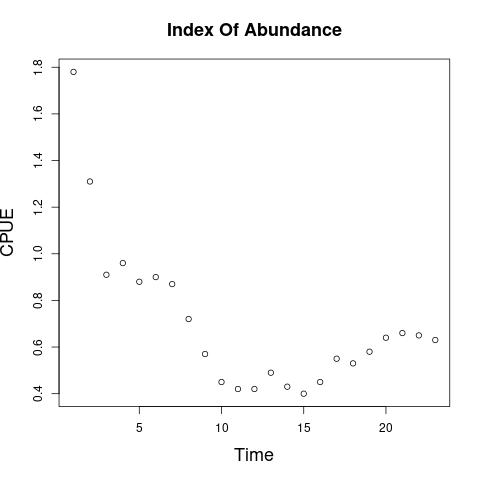
\includegraphics[width=0.45\textwidth]{./plots/hakeIndex.png}
%        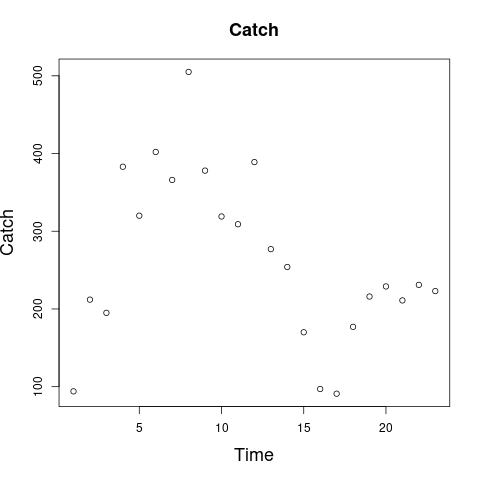
\includegraphics[width=0.45\textwidth]{./plots/hakeCatch.png}
%        \vspace{-1cm}
%	\caption{\label{hakeData}
%        \textit{left}: An index of abundance data, catch per unit effort (CPUE), for Namibian Hake from 1965 to 1987 \protect\shortcite{hilborn_ecological_1997}.
%        \textit{right}: The associated catch data for Namibian Hake over the same time period.
%        }
%\end{figure}
%
%%The observed 
%Indices are assumed to have multiplicative log-normal errors, and thus
%the following observation model arises naturally,
%%Pella Tomlinson
%\begin{align}
%I_t = q B_t e^\epsilon ~~~ \epsilon\sim N(0, \sigma^2).
%\end{align}
%%
%Above $q$ is often referred to as the ``catchability parameter''; it serves as the %represents the %$ is often refered to as the catchability parameter and the catchab
%proportionality constant mapping between the observed index of abundance and biomass.
%$\sigma^2$ models residual variation. Biologically speaking $q$ and $\sigma^2$
%are often treated as nuisance parameters with the ``biological parameters''
%entering the model through a process model on biomass.
%
%% 
%Biomass is assumed to evolve as an ODE; in this case I focus on the following
%form
%%
%\begin{equation}
%\frac{dB}{dt} = P(B(t); \bm{\theta}) - Z(t)B(t). \label{ode}
%\end{equation}
%%{\color{red}$C=FB$ to set up yield calculations later
%Here biomass is assumed to change in time by two processes, net production of
%biomass into the population, $P(B)$, and various sources of biomass removal, $Z$, from the 
%population. 
%%Generally production appears as a nonlinear function of existing biomass, 
%%and removals are assumed to be linear in biomass.
%
%%  %stock recruitment relationship (SRR). Recruitment 
%Firstly, the population grows through a production function, $P(B)$. Production
%in this setting is defined as the net biomass increase due to all reproduction
%and maturation processes.
%% accounting for all naturally occurring %no migration the population is assumed closed. 
%%sources of mortality other than the recorded fishing from humans. 
%The production function is assumed to be a parametric (generally non-linear) function 
%relating the current biomass of the population to an aggregate production 
%of biomass.
%
%%
%Secondly, the population decreases as biomass is removed by various sources that are 
%assumed to remove biomass linearly with biomass. Above, $Z(t)$, is an 
%aggregate rate of removal. When the fishing rate, $F(t)$, is the only source of removal 
%$Z(t)=F(t)$, however often models will also included other linear terms in $Z(t)$. 
%Commonly the rate of ``natural mortality'', $M$, is also included as an additional term 
%so that $Z(t)=M+F(t)$.
%
%%%
%%Secondly, the population decreases as biomass is removed due to catch, $C(t)$.
%%While catches (aka yields) are observable quantities \shortcite{pearson_documentation_1997}, %sen_sampling_1984,  
%%the model assumes that catch is proportional to biomass with the
%%proportionality constant representing the fishing rate, $F(t)$, so that $C(t)=F(t)B(t)$.
%From a management perspective a major goal of modeling is to accurately infer
%a quantity known as \emph{maximum sustainable yield} (MSY). One could maximize
%simple yield at a particular moment in time (and only for that moment) by
%fishing all available biomass in that moment. This strategy is penny-wise but
%pound-foolish (not to mention ecologically devastating) since it doesn't leave
%biomass in the population to reproduce in the future. We seek to fish in a way 
%that allows (or even encourages) future productivity in the population. This is 
%accomplished by maximizing the equilibrium level of catch over time. 
%Equilibrium yield is considered by replacing the steady state biomass ($\bar B$) 
%in the assumed form for catch, so that $\bar Y = F\bar B(F)$, where $\bar~$ 
%indicates a value at steady state.  
%%The steady state biomass is a function of $F$.
%%; we will see a specific example of this in
%%\mbox{Section (\ref{ptRef}).} 
%MSY is found by maximizing $\bar Y(F)$ with respect to
%$F$, and $F^*$ is the fishing rate at MSY. Going forward let $^*$ decorate any
%value derived under the condition of MSY.
%
%%
%Fisheries are very often managed based upon reference points %(RPs) 
%which serve as simplified heuristic measures of population behavior. The 
%mathematical form of RPs depends upon the model assumptions through the 
%production function. %({\color{red} cite}). 
%While a number of different RPs exist which describe the population in different
%(but related) ways, the most common RPs revolve around the concept of MSY (or robust
%ways of measuring MSY \shortcite{hilborn_pretty_2010,punt_management_2016}).
%Here the focus is primarily on the RPs $\frac{B^*}{\bar B(0)}$ and $F^*$ ($\frac{F^*}{M}$ when appropriate)
%for their pervasive use in modern fisheries \shortcite{punt_extending_2019}. %mangel_perspective_2013,
%
%%
%$F^*$ is the afore mentioned fishing rate which results in MSY. $\frac{B^*}{\bar B(0)}$
%is the depletion of the stock at MSY. That is to say $\frac{B^*}{\bar B(0)}$ describes
%the fraction of the unfished population biomass that will remain in the equilibrium
%at MSY. In general $F^*\in\mathbb{R}^+$ and \mbox{$\frac{B^*}{\bar B(0)}\in\left(0, 1\right)$,}
%however under the under the assumption of a two parameter production function production 
%models will be structurally unable to capture the full theoretical range of RPs. 
%%\shortcite{mangel_perspective_2013}.
%
%%
%Many of the most commonly used production functions depend only
%on two parameters. For example, the Schaefer model %{(\color{red}cite)}
%depends only on the biological parameters $r$ and $K$, and limits RP inference 
%so that under the Schaefer model $\left(F^*, \frac{B^*}{\bar B(0)}\right)\in \left(\mathbb{R}^+, \frac{1}{2}\right)$. 
%The two parameter Fox model \shortcite{fox_jr_exponential_1970} limits $\left(F^*, \frac{B^*}{\bar B(0)}\right)\in \left(\mathbb{R}^+, \frac{1}{e}\right)$. 
%Similarly the two parameter Cushing \shortcite{cushing_dependence_1971}, Beverton-Holt \shortcite[BH]{beverton_dynamics_1957}
%and Ricker \shortcite{ricker_stock_1954} production functions do not model the full theoretical space of
%RPs \shortcite{mangel_perspective_2013, yeakel_generalized_2015}.
%%curves are also two parameter
%%production functions that do not model the full theoretical space of
%%RPs \shortcite{mangel_perspective_2013}.
%
%%
%The bias-variance trade-off \shortcite{ramasubramanian_machine_2017} makes it
%clear that the addition of a third parameter in the production function will
%necessarily reduce estimation bias. However the utility of this bias reduction
%is still under debate because the particular mechanisms and behavior (direction and magnitude) %over relevant RPs %and mechanisms %behavior 
%of these biases for key management quantities %(and the mechanisms of inducing these biases) 
%are not fully understood or described. \shortciteA{lee_can_2012} provides some
%evidence that estimation of productivity parameters %, and thus RPs via \shortcite{mangel_perspective_2013},
%are dependent on biomass contrast as well as model specification. % as well as contrast in data %lacking contrast in biomass. 
%\shortciteA{conn_when_2010} comes to similar conclusions %about steepness estimation
%via calibration modeling techniques. These studies indicate important factors that
%contribute to inferential failure. However they do not offer mechanisms of model 
%failure, nor do their experimental designs allow for the control of different 
%types of model misspecification.
%% as those effects interact with the information content of a given biomass series.  
%
%%Despite this understanding of productivity estimation,
%%the implications have not been extended to a joint description of biases on the scale of
%%management RPs. % biases jointly.
%
%%The particular behaviors of these RP biases, 
%%and their relationship to each other, are not fully described.  
%
%%Add GOAL of understanding directionality and mechanism of bias.
%%Add claim of novelty by recognizing that bias is a function of RP, a flexible method of propagating estimation uncertainty and accounting for nonlinear bias patterns.
%
%%Together the general behavior of the PT model and the %pragmatic understandable 
%%simplicity of the Schaefer model make the PT/Schaefer pair an ideal setting for
%%beginning to understand the consequences of model misspecification on the
%%production function. 
%In this study I consider the behavior of inference when index data are simulated 
%from three parameter PT and Schnute production models, but the simulated data are fit 
%using intentionally misspecified two parameter logistic or BH production models.
%%
%The work begins with a derivation of RPs under the three parameter models. %PT model.
%A method is then presented for generating simulation designs based on the parametric 
%form of RPs which serves as a control on the nature of simulated model misspecification.
%% for analyzing inference under the two parameter model.
%%The parametric forms of RPs under the three parameter models are then inverted to develop a %PT model are then inverted to develop a
%%simulation setting for analyzing inference under the two parameter models. % Schaefer model as well as the BH. 
%Finally a Gaussian Process (GP) metamodel \shortcite{gramacy_surrogates_2020} 
%is constructed for exploration and analysis of RP biases.
%
%%
%A key insight of this approach is that bias is considered broadly across RP-space to
%uncover patterns and correlations between RPs. %f bias magnitude and direction. 
%%A flexible Gaussian Process (GP) meta-modeling approach is used to model bias 
%%patterns across RP-space. 
%The GP metamodel is explicit about trade-offs between RPs %to the surface bias tradeoffs to the surface to 
%so as to inform the full utility of reducing bias, as well as to suggest mechanisms for
%understanding what causes bias. Further, the effect of contrast on estimation
%is considered together with model misspecification. %alongside the effect of model misspecification.  
%
%%
%\section{Methods \label{meth}}
%%
%\subsection{Pella-Tomlinson Model}
%	%\begin{itemize}
%	%	%\item $\frac{dB}{dt} = P(B(t); \bm{\theta}) - F(t)B(t)$
%	%	%\item PT: $P(B; [r, K, \gamma]) = \frac{r B}{\gamma-1} \left(1-\frac{B}{K}\right)^{\gamma-1}$
%	%	%\item RP's (and analytically invert)
%	%	%\item fix PT plot
%	%	\item $\gamma=2$ $\Rightarrow$ Schaefer model (Schaefer RP)
%	%\end{itemize}
%
%%\subsection{PT Model}
%
%%
%%Below I present the three parameter Pella-Tomlinson (PT) family, which has a 
%The three parameter Pella-Tomlinson (PT) family has a convenient form that includes, among 
%others \shortcite{fox_jr_exponential_1970,rankin_alternative_2015}, the 
%logistic production function as a special case. %Under logistic production to form the Schaefer model. The 
%PT production function is parameterized so that $\bm{\theta} = [r, K, \gamma]$ 
%and the family takes the following form, 
%%Pella Tomlinson
%\begin{align}
%P_{p}(B; [r, K, \gamma]) = \frac{r B}{\gamma-1} \left(1-\left(\frac{B}{K}\right)^{(\gamma-1)}\right). \label{pt}
%\end{align}
%
%\clearpage
%
%%
%\begin{wrapfigure}{r}{0.45\textwidth} %[17]{r}[0pt]{0pt}%
%%\begin{figure}[h!]
%\vspace{-1cm}
%%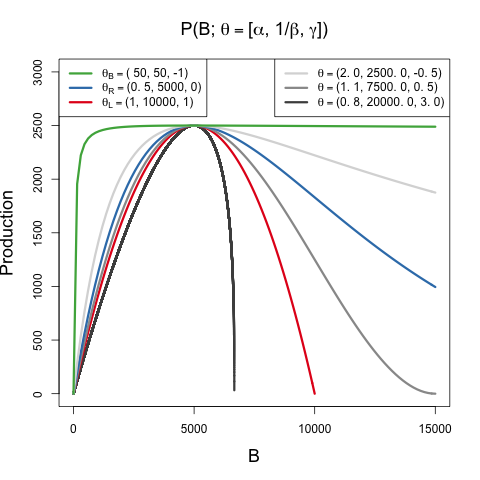
\includegraphics[width=0.5\textwidth]{plots/derisoSrr.png}
%%\begin{minipage}[h!]{0.64\textwidth}
%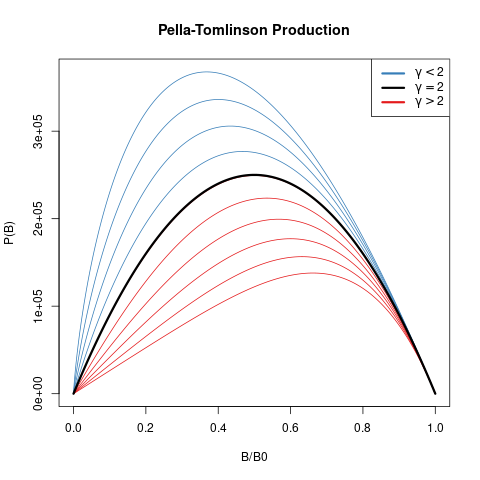
\includegraphics[width=0.49\textwidth]{../ptNew/g4PT.png}
%%\end{minipage}
%%\begin{minipage}[h!]{0.3\textwidth}
%\vspace{-1cm}
%%\hspace*{-1cm}
%\caption{
%%\onehalfspacing
%The Pella-Tomlinson production function plotted across a variety of parameter
%values. The special cases of Logistic production is shown in black, and the 
%left-leaning and right-leaning regimes are shown in blue and red respectively.
%}
%\label{SrrPT}
%%\end{minipage}
%\end{wrapfigure}
%%\end{figure}
%
%%
%$\gamma$ is a parameter which breaks PT out of the restrictive symmetry of the 
%logistic curve. In general $\gamma\in(1, \infty)$, with the logistic model
%appearing in the special case of $\gamma=2$, and the Fox model appearing as 
%a limiting case as $\gamma\to1$.
%%In the special case of $\gamma=2~$ Eq (\ref{pt}) 
%%collapses back to the logistic curve, however in general $\gamma\in(1, \infty)$.
%%
%%The parameters $r$ and $K$ maintain the same interpretation as 
%%they do in the logistic production function. In Figure (\ref{SrrPT}) PT recruitment 
%%is shown for a range of parameter values so as to demonstrate the various 
%%recruitment shapes that can be achieved by PT recruitment.  
%%
%The parameter $r$ controls the maximum reproductive rate of the population
%in the absence of competition for resources (i.e. the slope of production
%function at the origin). $K$ is the so called "carrying capacity" of the
%population. In this context the carrying capacity can be formally stated as
%steady state biomass in the absence of fishing \mbox{(i.e. $\bar B(0)=K$).}
%%
%In Figure (\ref{SrrPT}) PT recruitment is shown for a range of parameter values 
%so as to demonstrate the various recruitment shapes that can be achieved by PT 
%recruitment.  
%
%%{\color{red} And $\gamma$ is a parameter which adds 
%%flexibility to the family by allowing for compensatory or non-compensatory 
%%growth. (break symmetry... get better description) }
%
%%%\begin{wrapfigure}{r}{0.5\textwidth}
%%\begin{figure}[h!]
%%	\centering
%%	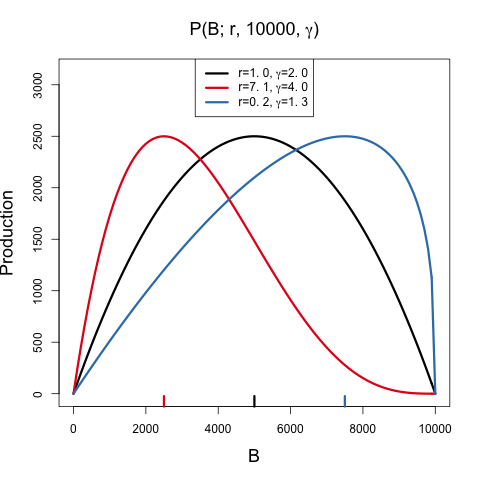
\includegraphics[width=0.49\textwidth]{./plots/srr1.1.png}	
%%	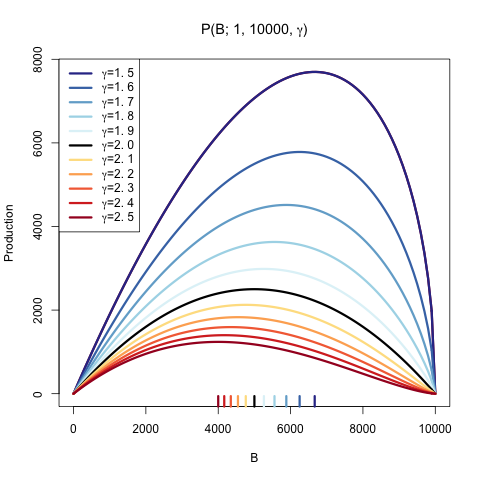
\includegraphics[width=0.49\textwidth]{./plots/srr2.png}
%%	\caption{\label{srrPT}
%%	(\emph{left}) PT production functions with parameters chosen so that MSY is consistent, but $\frac{B^*}{\bar B(0)}$ is less than $\frac{1}{2}$ (in red), greater than $\frac{1}{2}$ (in blue), or equal to $\frac{1}{2}$ (in black; logistic production function).
%%	(\emph{right}) PT production functions over a range of $\gamma$ values with the values of $r$ and $K$ fixed at 1 and 10,000 respectively.  
%%	}
%%\end{figure}
%%%\end{wrapfigure}
%
%%%
%%\clearpage
%
%%
%While the form of the PT curve produces some limitations \shortcite{fletcher_restructuring_1978}, %{(\color{red}cite)}, 
%importantly the % how $\gamma$ appears in PT still produces some limitations to the form of the production function 
%introduction of a third parameter allows enough flexibility to fully describe 
%the space of reference points used in management. To see this, the reference 
%points are analytically derived for the PT model below. % in the following section.
%
%%%
%%\begin{equation}
%%\frac{dB}{dt} = P - FB.
%%\end{equation}
%
%%
%\subsubsection{PT Reference Points}\label{ptRef}
%%
%With $B(t)$ representing biomass at time $t$, under PT production, the 
%dynamics of biomass are defined by the following ODE,
% 
%\begin{equation}
%\frac{dB}{dt} = \frac{r B}{\gamma-1} \left(1-\left(\frac{B}{K}\right)^{\gamma-1}\right) - FB. \label{dBdtPT}
%\end{equation}
%
%An expression for the equilibrium biomass is attained by setting Eq (\ref{dBdtPT}) 
%equal to zero, and rearranging the resulting equation to solve for $B$. 
%Thinking of the result as a function of $F$ gives, 
%%When thought of as a 
%%function of $F$ the following expression emerges,
%%{\color{red}Under Pella-Tomlinson SRR the equilibrium biomass can be written,}
%\begin{align}
%\bar B(F) = K\left(1-\frac{F(\gamma-1)}{r}\right)^{\frac{1}{(\gamma-1)}}. \label{BbarPT}
%\end{align}
%
%%By definition $B_0=K$. Alternatively, Setting $F=0$ in Eq(\ref{Beq}) makes it convenient to notice that $\bar B(0)=K$ to arrive at the same result
%At this point it is convenient to notice that $\bar B(0)=K$. The expression for 
%$B^*$ is given by evaluating Eq (\ref{BbarPT}) at $F^*$.
%%
%To get an expression for $F^*$, the equilibrium yield is maximized with respect to $F$,
%\begin{equation}
%F^* = \argmax_F F\bar B(F).
%\end{equation}
%%
%In the case of PT production this maximization can be done analytically, %. In this case maximization can proceed 
%by differentiating the equilibrium yield with respect to $F$ as follows,
%%
%\begin{align}
%\frac{d \bar{Y}}{dF} &= \bar B(F) + F \frac{d \bar B}{dF} \label{FderivPT}\\
%%\frac{d \bar B}{dF} &= -\frac{K}{\gamma-1}\left(\frac{\gamma-1}{r}\right)^{\frac{1}{\gamma-1}}F^{\frac{1}{\gamma-1}-1}\\
%\frac{d \bar B}{dF} &= -\frac{K}{r}\left(1-\frac{F(\gamma-1)}{r}\right)^{\frac{1}{\gamma-1}-1}\label{dBdFPT}.
%\end{align}
%
%%{\color{red}
%Setting Eq (\ref{FderivPT}) equal to 0, substituting $\bar B(F)$ and 
%$\frac{d \bar B}{dF}$ by Equations (\ref{BbarPT}) and (\ref{dBdFPT}) respectively, 
%and solving for $F$ produces the following expression for the fishing 
%rate required to produce MSY, %{\color{red}Below any quantity evaluated at MSY shall be decorated with $~^*$.}
%%
%\begin{align}
%F^* = \frac{r}{\gamma}%-1} \left(\frac{\gamma-1}{\gamma}\right)^{\gamma-1}. \label{Fmsy}
%\end{align}
%
%%
%Plugging the above expression for $F^*$ back into Eq (\ref{BbarPT}) gives the 
%following expression for biomass at MSY, 
%\begin{align}
%B^* = K\left(\frac{1}{\gamma}\right)^{\frac{1}{\gamma-1}} \label{BmsyPT}. %\left(1-\left(\frac{\gamma-1}{\gamma}\right)\right) \label{Bmsy}.
%\end{align}
%
%%
%The above derived expressions for $\bar B(0)$, $B^*$, and $F^*$ can then be used to 
%build a specific analytical form for the biological reference points in terms of only 
%productivity parameters.
%%%
%%By substituting the expressions given above for $B_0$, $B^*$, and $F^*$ into 
%%Eq(\ref{xizetaSimple}), $\xi$ and $\zeta$ can take a specific analytical form 
%%in terms of the biological model parameters. 
%%%given by substituting the expressions given in Eq(\ref{Fmsy}) 
%%%and Eq(\ref{Bmsy}) in Eq(\ref{xizetaSimple}).
%%%Eq(\ref{xizetaSimple}) can then take a specific analytical form in terms of the 
%%  %an expression for $\xi$ and $\zeta$ can be found in terms of model parameters.  
%\begin{align}\label{ptRP}
%&F^* = \frac{r}{\gamma}
%&\frac{B^*}{\bar B(0)} = \left(\frac{1}{\gamma}\right)^{\frac{1}{\gamma-1}}
%\end{align}
%
%%%{\color{red}demonstration of the restricted case with graph over RP space as used.}
%%
%%\subsection{Simulation Study \label{sim}}
%%
%%%
%%Indices of abundance are simulated from the three parameter PT production model 
%%over a grid of $F^*$ and $\frac{B^*}{\bar B(0)}$ values. These PT data are then 
%%fit with a two parameter Schaefer model. 
%%%$\gamma$ is then fixed to two so that the PT SRR reduces to the special case of logistic recruitment. 
%%%The restricted Schaefer model is then fit to the 
%%%simulated PT indices. 
%%
%%%%
%%%
%%%Let $\tilde~$ decorate any quantity that is derived under the restricted two 
%%%parameter SRR.\\ Collapse to the case of Schaefer. Similarly to Eq(\ref{
%%%logistic SRR}) setting $\gamma=2$ results in the equilibrium equations for the 
%%%restricted Schaefer model.  
%%% 
%%
%%%speaking it is not possible to analytically invert this  
%%Generating simulated indices of abundance from the PT model requires 
%%inverting the relationship between $\left(F^*, \frac{B^*}{\bar B(0)}\right)$, and 
%%$(r, \gamma)$. It is not generally possible to analytically invert this 
%%relationship for many three parameter production functions \shortcite{punt_extending_2019, schnute_analytical_1998}. %{(\color{red}cite Derizo paper)}. 
%%Most three parameter production functions lead to RPs that require expensive 
%%numerical methods to invert; more over the numerical inversion procedure can %is 
%%often be unstable. That said, for the case of PT this relationship is 
%%analytically invertible, and leads to the following relationship
%
%%
%\subsubsection{Simulation}
%
%%speaking it is not possible to analytically invert this  
%Generating simulated indices of abundance from the PT model requires
%inverting the relationship between $\left(F^*, \frac{B^*}{\bar B(0)}\right)$, and
%$(r, \gamma)$. It is not generally possible to analytically invert this
%relationship for many three parameter production functions \shortcite{punt_extending_2019, schnute_analytical_1998}. %{(\color{red}cite Derizo paper)}. 
%Most three parameter production functions lead to RPs that require expensive 
%numerical methods to invert; more over the numerical inversion procedure can %is 
%often be unstable. That said, for the case of PT this relationship is
%analytically invertible, and leads to the following relationship
%%
%\begin{align}
%&r = \gamma F^* 
%&\gamma = \frac{W\left(\frac{B^*}{\bar B(0)}\log\left(\frac{B^*}{\bar B(0)}\right)\right)}{\log\left(\frac{B^*}{\bar B(0)}\right)}. \label{gammaOfB}
%\end{align}
%%
%%Above $W_0$ is the principal branch of the Lambert product logarithm function. 
%%Above $W_{-1}$ is the lower branch of the Lambert product logarithm function. 
%Above $W$ is the Lambert product logarithm function. More details about this 
%derivation, and the Lambert product logarithm, are given in \mbox{Appendix (\ref{lambApp}).}
%
%%
%Using Eq. (\ref{gammaOfB}) to obtain production parameters, a PT production model 
%can be fully defined for any combination of the RPs $F^*$ and $\frac{B^*}{\bar B(0)}$.
%Since $K$ does not enter the RP calculation its value is fixed arbitrarily at 10000.
%
%%
%%\begin{itemize}
%%	\item introduce metamodeling idea
%%	%\item some design details
%%\end{itemize}
%%
%
%%$\sigma$ is fixed at the relatively small value of 0.01 to focus specifically on the
%%behavior of population parameters.
%
%%
%%The index residual standard deviation, $\sigma$, is fixed to the relatively 
%%small value of 0.01 to focus specifically on the behavior of productivity 
%%parameters.
%
%Indices of abundance are simulated from the three parameter PT production model
%broadly over the space of $F^*$ and $\frac{B^*}{\bar B(0)}$ via a space filling
%design as described in Section (\ref{lhs}). A small amount of residual variation, 
%$\sigma=0.01$, is added to the simulated index, and these data are then fit with a
%Schaefer model, at various degrees of misspecification, so as to observe the 
%effect of productivity model misspecification upon RP inference. 



%
%SCHNUTE
%



%
\subsection{Schnute Model}

%
The Schnute production function is a three parameter generalization of many of 
the most common two parameter production functions \shortcite{deriso_harvesting_1980, schnute_general_1985}. %\shortcit{deriso_harvesting_1980}. 
It can be written in the following form, with parameters $\alpha$, $\beta$, and $\gamma$,
%
\begin{align}
P_s(B; [\alpha, \beta, \gamma]) = \alpha B (1-\beta\gamma B)^{\frac{1}{\gamma}}.
\end{align}

%
\begin{wrapfigure}{r}{0.5\textwidth}
%\begin{figure}[h!]
%\begin{minipage}[h!]{0.64\textwidth}
\vspace{-0.6cm}
%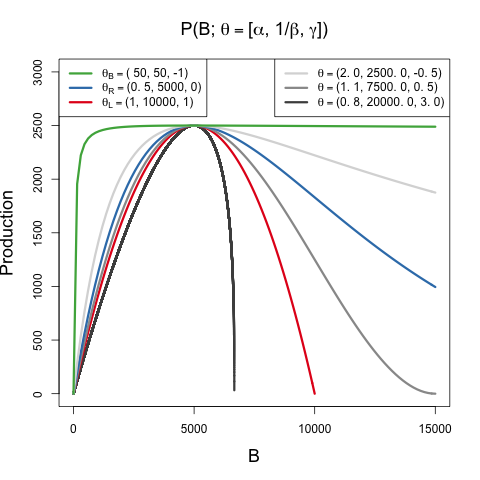
\includegraphics[width=0.5\textwidth]{plots/derisoSrr.png}
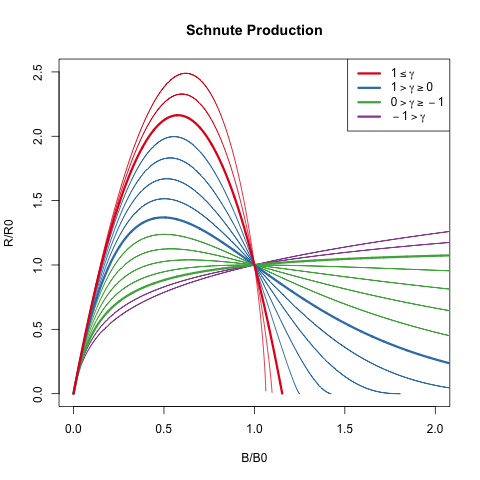
\includegraphics[width=0.49\textwidth]{../gpBias/g3.png}
\vspace{-1cm}
%\end{minipage}
%\begin{minipage}[h!]{0.3\textwidth}
\caption{
%\onehalfspacing
The Schnute production function plotted across a variety of parameter
values. Regimes of similarly behaving curves are grouped by color.
% BH-like, Ricker-like, and Logistic production are shown in
%green, blue, and red respectively.
}
\label{sRegimes}
%\end{minipage}
\end{wrapfigure}
%\end{figure}

%
The BH and Logistic production functions arise when $\gamma$ is fixed to -1 or 
1 respectively. The Ricker model is a limiting case as $\gamma\rightarrow0$. %\shortcite{schnute_general_1985}.
For $\gamma<-1$ a family of strictly increasing Cushing-like curves arise, 
culminating in linear production as $\gamma\to-\infty$. These special cases form
natural regimes of similarly behaving production functions as seen in Figure (\ref{sRegimes}).

%
The behavior of RP inference under the BH model is of particular interest due 
to the overwhelming popularity of the BH assumption in fisheries models.
%% 
%Inference of BH productivity parameters under a wide variety of data is of particular 
%interest due to the overwhelming popularity of the BH assumption in fisheries 
%models. 
Since Schnute production models can represent a quantifiably wide variety 
of possible productivity behaviors, they present an ideal simulation 
environment for inquiry of the reliability of inference under the BH 
assumption.

%
Under Schnute production, biomass dynamics evolve according to the following ODE, 
%
\begin{align}
\frac{dB}{dt} = P_s(B;\theta) - (M+F)B. \label{schnuteSimple}
\end{align}
%
This equation largely takes the same form as previously described, except 
that $P_s$ is the Schnute production function and natural mortality, $M$, is modeled 
explicitly here. % as opposed to  inclusion of natural mortality, $M$. 
Natural mortality models the instantaneous rate of mortality from all causes 
outside of fishing. Explicitly modeling natural mortality is not 
only a typical assumption of fisheries models, but is also key to the making 
RPs well defined over the relevant domain of $\gamma$.

%% matches the assumptions of typical fisheries models and 
%%
%In the Schaefer and PT models
%$M$ is modeled explicitly here  and $F$ are instantaneous rates of natural and fishing 
%mortality respectively. Unlike the PT model described above 

%with Schnute production simulates a
%wide variety of possible population productivity behaviors and provides an 

%
The derivation of RPs under Eq. (\ref{schnuteSimple}) follows a similar logic 
as under the PT model. An expression for equilibrium biomass is attained by 
setting $\frac{dB}{dt}=0$ and rearranging the resulting expression to solve 
for $B$ 
%
\begin{align}
\bar{B}(F) &= \frac{1}{\gamma \beta}\left(1-\left(\frac{M+F}{\alpha}\right)^\gamma\right).
\label{BsEq}
\end{align}

%
The above expression quickly yields $B_0$, $B^*$ by evaluation at $F=0$ and $F^*$ respectively,
%derive \bar B(F)
\begin{align}
B_0 &= \frac{1}{\gamma \beta}\left(1-\left(\frac{M}{\alpha}\right)^\gamma\right) \label{B0S}\\
\frac{B^*}{B_0} &= \frac{1-\left(\frac{M+F^*}{\alpha}\right)^\gamma}{ 1-\left(\frac{M}{\alpha}\right)^\gamma }. \label{BratS}
\end{align}

%
Attaining an expression for $F^*$ requires maximization of equilibrium 
yield, \mbox{$\bar{Y}=F\bar{B}(F)$}, with respect to $F$. Analytically maximizing 
proceeds by differentiating $\bar{Y}$ to produce
%
\begin{align}
\frac{d \bar{Y}}{dF} &= \bar B(F) + F \frac{d \bar B}{dF} \label{FderivS}\\
\frac{d \bar B}{dF} &= -\frac{1}{\beta}  \left(\frac{\left(\frac{M+F}{\alpha}\right)^\gamma}{F+M}\right)\label{dBdFS}.
\end{align}
%
Setting $\frac{d \bar{Y}}{dF}=0$, filling in the expressions for $\bar B(F)$ 
and $\frac{d \bar B}{dF}$, then rearranging to solve for $F^*$ is less 
yielding here than it was in the case of the PT model. This procedure falls 
short of providing an analytical solution for $F^*$ directly in terms of 
$\theta$, % $\alpha$, $\beta$, and $\gamma$, 
but rather shows that $F^*$ must respect the following expression,  
%
\begin{align}\label{FmsyS}
0 &= \frac{1}{\gamma} - \left(\frac{1}{\gamma} + \frac{F^*}{F^*+M}\right)\left(\frac{F^*+M}{\alpha}\right)^\gamma.  
\end{align}

%, although parameterizing slightly differently,
The lack of an analytical solution here is understood. 
\citeA[pg. 519]{schnute_analytical_1998} specifically points out that 
$F^*$ cannot be expressed analytically in terms of productivity parameters, 
but rather gives a partial analytical expression for the inverse relationship. 
Although parameterized slightly differently, \citeA{schnute_analytical_1998} 
derives expressions for $\alpha$ and $\beta$ as a function of RPs and $\gamma$. 
%rather suggests that a numerical solution 

%
%By working with the expressions $\frac{F^*}{M}$, $B_0$, $\frac{B^*}{B_0}$
Since RPs are left without a closed form expression, computing RPs from 
productivity parameters amounts to numerically solving the system formed by collecting the 
expressions (\ref{FmsyS}), (\ref{B0S}), and (\ref{BratS}).

%
\subsubsection{Simulation \label{sSim}}

%% 
%Inference of BH productivity parameters under a wide variety of data is of particular 
%interest due to the overwhelming popularity of the BH assumption in fisheries 
%models. Since Schnute production models can represent a quantifiably wide variety 
%of possible productivity behaviors, they present an ideal simulation 
%environment for inquiry of the reliability of inference under the BH 
%assumption.

%
For the purposed of simulation, it is not necessary to completely know 
%either of 
the precise relationships mapping RPs $\mapsto$ $\theta$ or $\theta$ $\mapsto$ 
RPs. Simulation only requires enough knowledge of these mappings to gather a list 
of $(\alpha, \beta, \gamma)$ tuples, for data generation under the Schnute model, 
and the corresponding RPs in some reasonable space-filling design over RP space. 

%
Similarly to \shortciteA{schnute_analytical_1998}, expressions %solving expressions 
(\ref{FmsyS}) and (\ref{B0S}) are solved for $\alpha$ and $\beta$ respectively. 
This leads to the partial mapping 
$\big(F^*, B_0\big) \mapsto \big(\alpha(\cdot, \gamma), ~\beta(\cdot, \cdot, \gamma)\big)$ 
in terms of RPs and $\gamma$. 
% yields a partial mapping from 
%$\big(F^*, B_0\big) \mapsto \big(\alpha(\cdot, \gamma), ~\beta(\cdot, \cdot, \gamma)\big)$.
By further working with Eq. (\ref{BratS}), to identify $\gamma$, the following 
system is obtained,
%
\begin{align}
%\frac{B^*}{B_0} &= \frac{1-\left(\frac{M+F^*}{\alpha}\right)^\gamma}{ 1-\left(\frac{M}{\alpha}\right)^\gamma } \\
\alpha &= (M+F^*)\left(1+\frac{\gamma F^*}{M+F^*}\right)^{1/\gamma} \nonumber\\
\beta &= \frac{1}{\gamma B_0}\left(1-\left(\frac{M}{\alpha}\right)^\gamma\right) \label{abgSys}\\
\frac{B^*}{B_0} &= \frac{1-\left(\frac{M+F^*}{\alpha}\right)^\gamma}{ 1-\left(\frac{M}{\alpha}\right)^\gamma } \nonumber.
\end{align}

%
For a population experiencing natural mortality $M$, by fixing $F^*$, 
$B_0$, and $\frac{B^*}{B_0}$ %$B^*$ % 
the above system can fully specify $\alpha$ and $\beta$ for a given $\gamma$. % if only $\gamma$ were further isolated
Notice for a given $\gamma$ a cascade of closed form solutions for $\alpha$ 
and $\beta$ can be obtained. First $\alpha(\gamma)$ can be computed, and then 
$\beta(\alpha(\gamma), \gamma)$ can be computed. If $\alpha(\gamma)$ is filled 
back into the expression for $\frac{B^*}{B_0}$, the system collapses into 
a single onerous expression for $\frac{B^*}{B_0}(\alpha(\gamma), \gamma)$. 
For brevity, define the function \mbox{$\zeta(\gamma)=\frac{B^*}{B_0}\big(\alpha(\gamma), \gamma, F^*, M\big)$} based on Eq. (\ref{BratS}). 

% %possible;
Inverting $\zeta(\gamma)$ for $\gamma$, and computing the cascade of 
$\alpha(\gamma)$, and then $\beta(\alpha(\gamma), \gamma)$, fully defines the 
Schnute model for a given $(\frac{F^*}{M}, \frac{B^*}{B_0})$. However
inverting $\zeta$ accurately is extremely difficult. Inverting $\zeta$ 
analytically is not feasible, and numerical methods for inverting 
$\zeta$ are unstable and can be computationally expensive. 
%Numerically inverting $\zeta$ quickly becomes 
%prohibitively expensive, and solutions are often still unreliable. 
%
Rather than numerically invert precise values of $\zeta(\gamma)$, $\gamma$ is 
sampled so that the overall simulation design is space filling as described in 
Section (\ref{sLHS}).

%
Each design location defines a complete Schnute production model with the given 
RP values. Indices of abundance are simulated from the Schnute model at each design
location, a small amount of residual variation, $\sigma=0.01$, is added to the 
simulated index, and the data are then fit with a misspecified BH production model. 
The design at large captures various degrees of model misspecification relative 
to the BH model, so as to observe the effect of productivity model misspecification 
upon RP inference.

%$\sigma$ is fixed at the relatively small value of 0.01 to focus specifically on the
%behavior of population parameters.

%
%The index residual standard deviation, $\sigma$, is fixed to the relatively 
%small value of 0.01 to focus specifically on the behavior of productivity 
%parameters.

%Indices of abundance are simulated from the three parameter PT production model
%broadly over the space of $F^*$ and $\frac{B^*}{\bar B(0)}$ via a space filling
%design as described in Section (\ref{lhs}). A small amount of residual variation, 
%$\sigma=0.01$, is added to the simulated index, and these data are then fit with a
%Schaefer model, at various degrees of misspecification, so as to observe the
%effect of productivity model misspecification upon RP inference.
%
%%
%{\color{red}
%%
%Using Eq. (\ref{gammaOfB}) to obtain production parameters, a PT production model 
%can be fully defined for any combination of the RPs $F^*$ and $\frac{B^*}{\bar B(0)}$.
%Since $K$ does not enter the RP calculation its value is fixed arbitrarily at 10000.
%
%
%
%Indices of abundance are simulated from the three parameter PT production model
%broadly over the space of $F^*$ and $\frac{B^*}{\bar B(0)}$ via a space filling
%design as described in Section (\ref{lhs}). These PT indices are then fit with a
%Schaefer model, at various degrees of misspecification, so as to observe the 
%effect of productivity model misspecification upon RP inference. 
%}


%\clearpage	
%
\subsection{Latin Hypercube Sampling \label{lhs}}

%\begin{itemize}
%	{\color{red}
%	\item a quick lit review of space filling designs}
%	
%	\item LHS doesn’t preclude two points located nearby one another.
%	\item good projective properties
%	\item maximin designs are often concentrated in the corners (edges) of the design region
%
%	%\item goal of space filling
%	\item \shortcite{gramacy_surrogates_2020} The goal is to guarantee a certain degree of spread in the design, 
%	while otherwise enjoying the properties of a random uniform sample.
%	\item \shortcite{devon_lin_latin_2015}  Construction and properties.
%	\item \shortcite{stein_large_1987} large sample props. 
%	\item Monotonicity: Latin hypercube sampling yields a smaller variance of the sample mean than simple random sampling
%	\item \shortcite{owen_central_1992} CLT
%\end{itemize}

%
The goal of space filling design in this setting is to extend the notion of the 
random sample (and its desirable parameter estimation properties) across the 
simulated RP domain so as to represent the simulated space as well as possible \shortcite{gramacy_surrogates_2020}.
The simple random sample is the classical approach to unbiased parameter 
estimation, however simple randomness is patchy, often sampling some regions 
of design space quite densely, while leaving other regions of design space empty. 
Space filling designs aim to preserve (or enhance) parameter estimation properties 
across the simulated domain \shortcite{devon_lin_latin_2015, stein_large_1987}, 
while constraining samples to be spaced in some notion of spread over the entire space.
Latin hypercube sampling \shortcite[LHS]{mckay_comparison_2000} is among the most 
foundational of space filling designs used in computer experiments.

%
%\begin{figure}[h!]
%\centering [width=0.96\textwidth]
\begin{wrapfigure}{r}{0.5\textwidth}
%\vspace{-2.9cm}
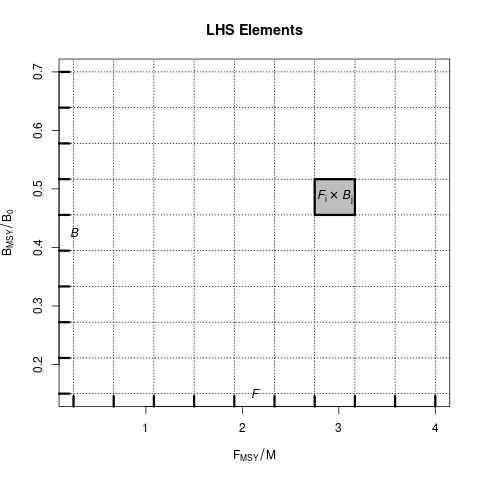
\includegraphics[width=0.49\textwidth]{../gpBias/designGrid.png}
\caption{ LHS grids. Intersecting $\mathcal{F}$ and $\mathcal{B}$ produces $n^2$
cells; a particular cell $\mathcal{F}_i\times\mathcal{B}_j$ is shown in grey. 
{\color{red} Maybe just show points.}
}
\end{wrapfigure}

%%
%A Latin hypercube sample (LHS) of size $n$, in an $m$ dimensional space, samples
%uniformly among uniform grids of size $n$ in each dimension of the design space. By
%intersecting the grids of each dimension, $n^m$ cells are produced, from which
%a total of $n$ samples are taken. Crucially only one sample is taken from a given element
%of each grid in each dimension so as to reduce clumping of the $n$ samples
%across the design space.

%
A LHS of size $n$, in the 2 dimensional space defined 
by RPs, distributes samples so as to spread points across a design region in a 
broadly representative way. A LHS design extends the notion of a univariate 
random uniform sample across multiple dimensions so that each margin of the design 
space enjoys a uniform distribution. 

%
LHS designs achieve this notion of uniformity by first partitioning each dimension 
of the design space into regular grids of size $n$. By intersecting the grids 
of each dimension, cells are produced that evenly partition the design space. 
In two dimensions $n^2$ cells are produced, from which a total of $n$ samples 
are taken. Crucially only one sample is taken from a given element of each grid 
in each dimension so as to reduce clumping of the $n$ samples across the design space.



%%, $n^m$ cells are produced, from which
%%LHS designs achieves this notion of uniformity %, across say $m$ dimensions, 
%by partitioning the space, and then sampling uniformly within a uniform partitions 
%so that each.
%The design region is partitioning by intersecting regular grids of, size $n$, in 
%each dimension so that $n^m$ cells are produced (where $m$ is the number of dimensions of the design shape) 
%
%the space of RPs so that 
 


%%
%%PELLA
%%
%
%
%%
%\subsubsection{PT Design}
%
%%
%Letting $\mathcal{F}$ and $\mathcal{B}$ be regular grids, of size $n=100$, on
%\mbox{$F^*\in(0.1, 0.7)$} and \mbox{$\frac{B^*}{B_0}\in(0.2, 0.6)$}
%respectively, a LHS design of size 100 is collected among the cells produced by
%$\mathcal{F}\times\mathcal{B}$. 
%
%%
%Each of the sampled LHS design locations represent a unique PT model with the 
%sampled RP values. Since the relationship mapping RPs analytically to productivity 
%parameters can be found for the PT model, LHS designs the the PT model are 
%computed directly in RP space and Eq. (\ref{gammaOfB}) is used to map the 
%sampled RP design locations to PT productivity parameters. 
%%created by samples 1 point in $n$ of the $n^2$ cells produced by
%%$\mathcal{F}\times\mathcal{B}$. 
%%
%%If $\mathcal{F}$ is an equally spaced grid of size $n$ for 
%%$\frac{F^*}{M}\in(0.25, 4)$, and letting $\mathcal{B}$ be an 
%%equally spaced grid of size $n$ for $\frac{B^*}{B_0} \in (0.15, 0.7)$. 
%%$\mathcal{F}$
%%
%
%%%
%%Each of the sampled LHS design locations represent a unique PT model with the 
%%sampled RP values. The productivity parameters of the PT, at each design location,
%%are obtained by applying Eq. (\ref{gammaOfB}). Since $K$ does not enter the RP 
%%calculation its value is fixed arbitrarily at 10000. The value of $q$ is fixed 
%%at a typically small value of 0.0005. $\sigma$ is fixed at the relatively small 
%%value of 0.01 to focus specifically on the behavior of population parameters. 
%%These parameters fully specify the PT model for the purposes of generating 
%%index data for each $\left(F^*, \frac{B^*}{\bar B(0)}\right)$ pair.
%
%%productivity parameters 
%%of the data generating PT 
%%model are obtained, and PT index of abundance data can be   for the purpose of generating index of abundance 
%%Given the analytical relationship between the RPs and the productivity parameters
%%$r$, $K$, and $\gamma$ for the PT model, obtaining a uniform LHS sample among
%%$\mathcal{F}\times\mathcal{B}$ requires a tactful navigation of the system of
%%equations seen in Eq. (\ref{abgSys}). The LHS grid setup and rough sampling strategy
%%can be seen in Figure (\ref{sudoGrid}).
%
%%%
%%\begin{figure}[h!]
%%%\centering
%%%\begin{minipage}[h!]{0.49\textwidth}
%%        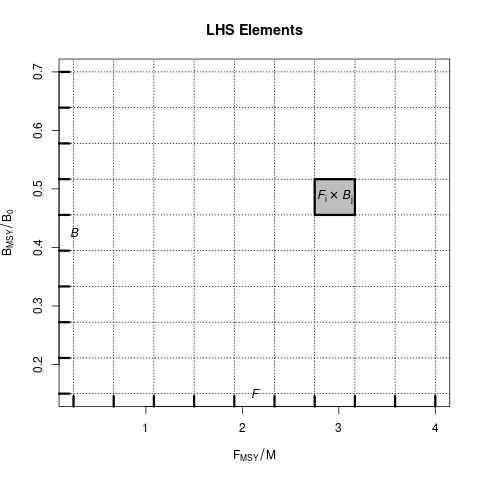
\includegraphics[width=0.96\textwidth]{../gpBias/designGrid.png}
%%%\end{minipage}
%%%\begin{minipage}[h!]{0.49\textwidth}
%%%\begin{itemize}
%%%        \item[] \hspace*{-1cm}Given $B_0$, $M$, and $F^*$:
%%%        \item[1)] Draw $\gamma^* \sim \gamma|F^*, M$.
%%%        \item[2)] Compute $\frac{B^*}{B_0} = \zeta(\gamma^*)$
%%%        \item[3)] Compute $\alpha^* = \alpha(\gamma^*, F^*, M)$
%%%        \item[4)] Compute $\beta^* = \beta(\alpha^*, \gamma^*, M, B_0)$
%%%\end{itemize}
%%%\end{minipage}
%%\caption{
%%LHS grids. Intersecting $\mathcal{F}$ and $\mathcal{B}$ produces $n^2$
%%cells; a particular cell $\mathcal{F}_i\times\mathcal{B}_j$ is shown in grey.
%%%($right$) An outline of the sampling procedure for $\gamma$ (and associated
%%%quantities) given $B_0$, $M$, and $F^*$. %$\mathcal{F}_i$.
%%\label{sudoGrid}}
%%\end{figure}
%%
%%%
%%Indices are generated under the following conditions. Data are simulated at
%%each point on the grid $\mathcal{F}\times\mathcal{B}$, with $F^*\in\mathcal{F}$
%%and $\frac{B^*}{\bar B(0)}\in\mathcal{B}$, where $\mathcal{F}=\{0.1, 0.2, ..., 0.7\}$
%%and $\mathcal{B}=\{0.2, 0.3, ..., 0.6\}$ as seen in Figure (\ref{rpGrid}).
%%These ranges of values for $F^*$ and $\frac{B^*}{\bar B(0)}$ are selected to
%%include a wide range of values thought to reflect many commonly assessed fisheries.
%%%commonly  of most commonly assessed fish species {\color{red}cite}. 
%%The red X's in Figure (\ref{rpGrid}) show four simulation locations where the
%%Schaefer model is misspecified to a large degree and will be considered in more
%%detail in \mbox{Section(\ref{flat}).} For each $\left(F^*, \frac{B^*}{\bar B(0)}\right)$,
%%the associated pair $(r, \gamma)$ are computed from \mbox{Eq (\ref{rg}).} Since $K$
%%does not enter the RP calculation its value is fixed arbitrarily at 10000.  %A relatively large value of $K$ is selected to allow a full range of population dynamics t
%%The value of $q$ is fixed at a typically small value of 0.0005. $\sigma$ is
%%fixed at the relatively small value of 0.01 to focus specifically on the
%%behavior of population parameters. These parameters fully specify the PT
%%model for the purposes of generating index data for each $\left(F^*, \frac{B^*}{\bar B(0)}\right)$ pair.



%
%SCHNUTE
%


%
\subsubsection{Schnute Design \label{sLHS}}

%%
%A Latin hypercube sample (LHS) of size $n$, in an $m$ dimensional space, samples 
%uniformly among uniform grids of size $n$ in each dimension of the design space. By 
%intersecting the grids of each dimension, $n^m$ cells are produced, from which 
%a total of $n$ samples are taken. Crucially only one sample is taken from a given element 
%of each grid in each dimension so as to reduce clumping of the $n$ samples 
%across the design space.  


%a LHS samples 1 point in $n$ of the $n^2$ cells produced by $\mathcal{F}\times\mathcal{B}$.
%
%If $\mathcal{F}$ is an equally spaced grid of size $n$ for 
%$\frac{F^*}{M}\in(0.25, 4)$, and letting $\mathcal{B}$ be an 
%equally spaced grid of size $n$ for $\frac{B^*}{B_0} \in (0.15, 0.7)$. 
%$\mathcal{F}$
% 
%$\alpha$, $\beta$, and $\gamma$, obtaining a uniform LHS sample among 
%$\mathcal{F}\times\mathcal{B}$ requires a tactful navigation of the system of 
%equations seen in Eq. (\ref{abgSys}). The LHS grid setup and rough sampling strategy 
%can be seen in Figure (\ref{sudoGrid}).
%%
%\begin{figure}[h!]
%\centering
%\begin{minipage}[h!]{0.49\textwidth}
%	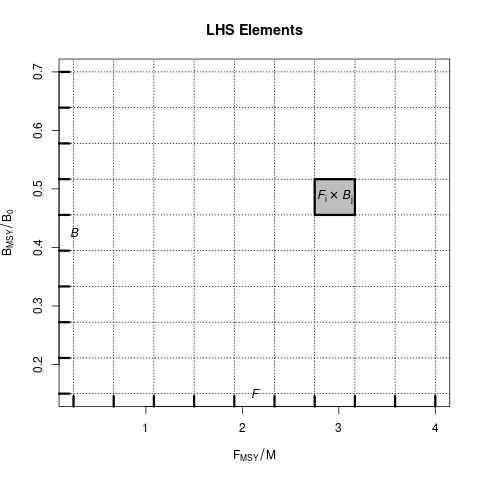
\includegraphics[width=0.96\textwidth]{../gpBias/designGrid.png}
%\end{minipage}
%\begin{minipage}[h!]{0.49\textwidth}
%\begin{itemize}
%	\item[] \hspace*{-1cm}Given $B_0$, $M$, and $F^*$:
%	\item[1)] Draw $\gamma^* \sim \gamma|F^*, M$.
%	\item[2)] Compute $\frac{B^*}{B_0} = \zeta(\gamma^*)$
%	\item[3)] Compute $\alpha^* = \alpha(\gamma^*, F^*, M)$
%        \item[4)] Compute $\beta^* = \beta(\alpha^*, \gamma^*, M, B_0)$
%\end{itemize}
%\end{minipage}
%\caption{
%($left$) LHS grids. Intersecting $\mathcal{F}$ and $\mathcal{B}$ produces $n^2$ 
%cells; a particular cell $\mathcal{F}_i\times\mathcal{B}_j$ is shown in grey. 
%($right$) An outline of the sampling procedure for $\gamma$ (and associated 
%quantities) given $B_0$, $M$, and $F^*$. %$\mathcal{F}_i$.
%\label{sudoGrid}}
%\end{figure}
%
%%
%\clearpage
%%{\color{red}Connect overview to details below}
%%Since inverting $\zeta(\gamma)$ is not feasible, sampling $\gamma$ so as to 
%%produce a LHS design  

%

%dion RPs and directly mapping those sampled RP design locations to the Schnute model's productivity parameters is 
%not possible. However different approach for simulation design in RP space is  mapping RPs to productivity 
%parameters is required for the Schnute model. 



%RPs $\mapsto$ $\theta$ or $\theta$ $\mapsto$RPs
Due to the lack of an analytical relationship mapping RPs $\mapsto$ $\theta$, 
analogous to the PT model's Eq. (\ref{gammaOfB}), producing a LHS design 
over Schnute RPs requires a more tactful approach.
The structured relationship between the RPs and productivity parameters, 
described in Section (\ref{sSim}), allows an approximate LHS to be obtained by 
a careful navigation of the system of equations seen in Eq. (\ref{abgSys}).

%
\begin{wrapfigure}{r}{0.5\textwidth}
\vspace{-0.5cm}
\begin{itemize}
        \item[] \hspace*{-1cm}Given $B_0$, $M$, and $F^*$:
        \item[1)] Draw $\gamma^* \sim \gamma|F^*, M$.
        \item[2)] Compute $\frac{B^*}{B_0} = \zeta(\gamma^*)$
        \item[3)] Compute $\alpha^* = \alpha(\gamma^*, F^*, M)$
        \item[4)] Compute $\beta^* = \beta(\alpha^*, \gamma^*, M, B_0)$
\end{itemize}
\vspace{-0.5cm}
\caption{ An outline of the sampling procedure for $\gamma$ 
%(and associated quantities) 
given $B_0$, $M$, and $F^*$.
}
\end{wrapfigure}

%
Under the Schnute model, let $\mathcal{F}$ and $\mathcal{B}$ represent regular grids on
%Letting $\mathcal{F}$ and $\mathcal{B}$ be equally spaced grids, of size $n$, on 
\mbox{$\frac{F^*}{M}\in(0.25, 4)$} and \mbox{$\frac{B^*}{B_0}\in(0.15, 0.7)$}
respectively which can serve as the scaffolding for computing an approximate LHS.

%
Since it is not practical to invert $\zeta(\gamma)$, a uniform sample in 
$\frac{B^*}{B_0}$ can be obtained by modeling $\gamma$ as a random 
variable, with realization $\gamma^*$, and thinking of $\zeta(\gamma)$ as its 
cumulative distribution function (CDF). The aim is to model $\gamma$ as an 
easily sampled random variable with a CDF that closely approximates $\zeta$, so 
that $\zeta(\gamma^*)\dot\sim U(\zeta_{min},1)$ as closely as possible. There 
may be many good models for the distribution of $\gamma$, but in this setting 
the following distribution is very effective,
%
\begin{align}
\gamma \sim \zeta_{min}\delta(\gamma_{min}) + t(\mu, \sigma, \nu)\bm{1}_{\gamma>\gamma_{min}}. \label{mixT}
\end{align}

%
%\clearpage

%
\begin{wrapfigure}{r}{0.5\textwidth}
\vspace*{-1cm}
%\begin{figure}[h!]
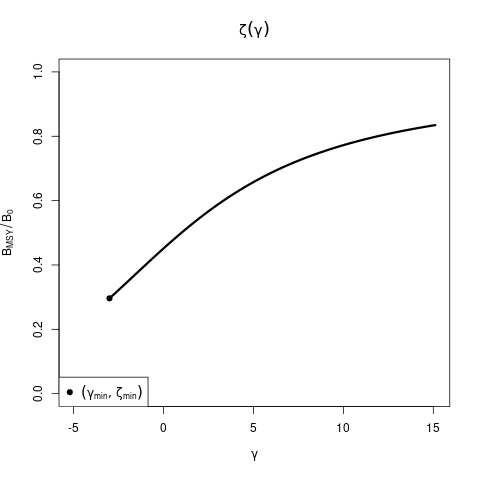
\includegraphics[width=0.5\textwidth]{../gpBias/zeta.png}
\vspace*{-1.3cm}
\caption{$\zeta(\gamma)$ Plotted for $F^*=0.1$ and $M=0.2$. The point 
$(\gamma_{min}, \zeta_{min})$ shows the lowest biologically meaningful 
value of $\gamma$; below which productivity is negative.}
%\end{figure}
\end{wrapfigure}
 
%
Above, $t$ is the density of the three parameter location-scale family Student's $t$ 
distribution with location $\mu$, scale $\sigma$, and degrees of freedom $\nu$. 
$\bm{1}_{\gamma>\gamma_{min}}$ is an indicator function that serves to truncate the 
Student's $t$ distribution at the lower bound $\gamma_{min}$. 
$\delta(\gamma_{min})$ is the Dirac delta function evaluated at $\gamma_{min}$, 
which is scaled by the known value $\zeta_{min}$; this places probability mass 
$\zeta_{min}$ at the point $\gamma_{min}$. Since sampling from a Student's $t$ 
distribution is readily doable, sampling from a truncated Student's $t$ mixture 
only requires slight modification. 

%$~$\\$~$\\
Let $T$ be the CDF of the modeled distribution of $\gamma$. Since the point 
$(\gamma_{min}, \zeta_{min})$ is known from the dynamics of the Schnute model 
at a given RP, full specification of Eq. (\ref{mixT}) only requires determining 
the values for $\mu$, $\sigma$, and $\nu$ which make $T$ best approximate 
$\zeta(\gamma)$. Thus, the values of $\mu$, $\sigma$, and $\nu$ are chosen by 
minimizing the $L^2$ distance between $T(\gamma)$ and $\zeta(\gamma)$.
%Letting $T$ be the CDF of the modeled distribution of $\gamma$, the values of $\mu$, $\sigma$, and $\nu$ are chosen by minimizing the $L^2$ distance between $T(\gamma)$ and $\zeta(\gamma)$.
%{\gamma_{min}}^{\gamma_{0.9}}
\begin{align}
[\hat\mu, \hat\sigma, \hat\nu]=\underset{{[\mu, \sigma, \nu]}}{\arg\min}\int_\Gamma \big(T(\gamma; \mu, \sigma, \nu) - \zeta(\gamma)\big)^2 d\gamma
\end{align}  

%%
%\begin{figure}
%\begin{minipage}[h!]{0.49\textwidth}
%\setstretch{1.5}

%
\clearpage
%
\begin{wrapfigure}{R}{0.5\textwidth}
	%\vspace{-0.5cm}
	\vspace{-1cm}
	\begin{minipage}{0.5\textwidth}
      		\begin{algorithm}[H]
			\caption{LHS of size $n$ on rectangle $R$.}
			\label{lhsAlg}
			\begin{algorithmic}[1]
			\Procedure{$LHS_n(R)$}{}
			\State Define $n$-grids $\mathcal{F}, \mathcal{B}\in R$
			\For{each grid element $i$}
			\State Draw $\frac{F^*}{M} \sim Unif(\mathcal{F}_i)$
			\State Compute $[\hat\mu, \hat\sigma, \hat\nu]$ given $F^*~\&~M$
			\While {$\mathcal{B}_j$ not sampled}
				\State Draw $\gamma^* \sim T(\gamma|\hat\mu, \hat\sigma, \hat\nu)$
				\State Compute $\zeta^* = \zeta(\gamma^*)$
				\State Compute $j$ such that $\zeta^*\in\mathcal{B}_j$
				%\State Compute $\alpha^* = \alpha(\gamma^*, F^*, M)$ 
				%\State Compute $\beta^* = \beta(\alpha^*, \gamma^*, M, B_0)$	
				%\State \mbox{Save $(\frac{F^*}{M}, \zeta^*)\Leftrightarrow(\alpha^*, \beta^*, \gamma^*)$ in $\mathcal{F}_i\times\mathcal{B}_j$} 
			\EndWhile
			\State Compute $\alpha^* = \alpha(\gamma^*, F^*, M)$ 
			\State Compute $\beta^* = \beta(\alpha^*, \gamma^*, M, B_0)$	
			\State \mbox{Save $(\frac{F^*}{M}, \zeta^*)\Leftrightarrow(\alpha^*, \beta^*, \gamma^*)$ in $\mathcal{F}_i\times\mathcal{B}_j$} 
			\EndFor
			\EndProcedure
			\end{algorithmic}
		\end{algorithm}
	\end{minipage}
\end{wrapfigure}
%{\color{red}Connect $T(\gamma|\hat\mu, \hat\sigma, \hat\nu)$ to overall algorithm.}


%Fitting the distribution $T(\gamma|\hat\mu, \hat\sigma, \hat\nu)$ for 
%use generating $\gamma^*$ values at a specific $F^*$ and $M$ releases the 
%need to invert $\zeta$. 
%using $T(\gamma|\hat\mu, \hat\sigma, \hat\nu)$ 
%Furthermore, $T(\gamma|\hat\mu, \hat\sigma, \hat\nu)$, taken together with 
The distribution $T(\gamma|\hat\mu, \hat\sigma, \hat\nu)$ is fit for use in 
generating $\gamma^*$ random variates at a specific $F^*$ and $M$. This approximation 
releases the need to invert $\zeta$ w.r.t $\gamma$ by using samples of $\gamma^*$ values to 
generate approximatly uniform samples of $\zeta(\gamma^*)$. By sampling approximatly 
uniform $\zeta(\gamma^*)$ random variates in this way, and making use of the structure in Eq. (\ref{abgSys}), 
%allows for the collection of 
an approximate LHS sample can be collected via Algorithm (\ref{lhsAlg}). %Figure (\ref{sudoCode}). 

%
$\frac{F^*}{M}$ is drawn uniformly from $\mathcal{F}_i$. Conditioning on the 
sample of $F^*$, and $M$, $T(\gamma|\hat\mu, \hat\sigma, \hat\nu)$ is fit and 
$\gamma^*$ is sampled. $\zeta^*$ is then computed and placed into the appropriate
grid element $\mathcal{B}_j$. Given $\gamma^*$, the cascade $\alpha(\gamma^*)$, 
and $\beta(\alpha(\gamma^*), \gamma^*)$, can be computed. The algorithm 
continues until all of the design elements, $(\frac{F^*}{M}, \zeta^*)\Leftrightarrow(\alpha^*, \beta^*, \gamma^*)$,
have been computed for all $i\in[1,...,n]$.

%design elements, $(\frac{F^*}{M}, \zeta^*)\Leftrightarrow(\alpha^*, \beta^*, \gamma^*)$,
%have been computed for all $i\in[1,...,n]$.


%With $T(\gamma|\hat\mu, \hat\sigma, \hat\nu)$ fitted for a specific $F^*$ 
%and $M$, Eq. (\ref{abgSys}) can be navigated to  

%\end{minipage}
%\begin{minipage}[h!]{0.49\textwidth}
%%\begin{figure}
%%\begin{wrapfigure}{r}{0.8\textwidth}
%%\vspace*{-1cm}
%\begin{itemize}
%	%\setlength\itemsep{-0.5em}
%	\item[$\forall i$:]
%	\item[1)] Draw $\frac{F^*}{M} \sim Unif(\mathcal{F}_i)$.
%	\item[2)] Compute $[\hat\mu, \hat\sigma, \hat\nu]$ given $F^*$ and $M$.
%	\item[3)] Draw $\gamma^* \sim T(\gamma|\hat\mu, \hat\sigma, \hat\nu)$.
%	\item[4)] Compute $\zeta^* = \zeta(\gamma^*)$.
%	\item[5)] Compute $j$ such that $\zeta^*\in\mathcal{B}_j$.
%	\item[6)] If $\mathcal{B}_j$ is already sampled, go to 3).
%	\item[7)] Compute $\alpha^* = \alpha(\gamma^*, F^*, M)$. 
%	\item[8)] Compute $\beta^* = \beta(\alpha^*, \gamma^*, M, B_0)$.	
%	\item[9)] \mbox{Save $(\frac{F^*}{M}, \zeta^*)\Leftrightarrow(\alpha^*, \beta^*, \gamma^*)$ in $\mathcal{F}_i\times\mathcal{B}_j$.} 
%	%\\ Otherwise go to 1).%If $\mathcal{B}_j$ is not sampled: save $\zeta^*$.\\ Otherwise go to 3). %
%\end{itemize}
%%\end{wrapfigure}
%\caption{Sudo-code procedure for LHS sampling in $\mathcal{F}\times\mathcal{B}$.}
%\label{sudoCode}
%\end{minipage}
%\end{figure}
%\noindent
%%\vspace*{0.5cm}
%The algorithm continues until all of the 


%%
%\begin{wrapfigure}{R}{0.5\textwidth}
%	\begin{minipage}{0.5\textwidth}
%      		\begin{algorithm}[H]
%			\caption{}
%			\label{lhsAlg}
%			\begin{algorithmic}[1]
%			\Procedure{$LHS_n(x,y)$}{}
%			\State Define $n$-grids $\mathcal{F}\in x$ and $\mathcal{B}\in y$
%			\For{each grid element $i$}
%			\State Draw $\frac{F^*}{M} \sim Unif(\mathcal{F}_i)$
%			\State Compute $[\hat\mu, \hat\sigma, \hat\nu]$ given $F^*$ and $M$
%			\While {any $\mathcal{B}$ not sampled}
%				\State Draw $\gamma^* \sim T(\gamma|\hat\mu, \hat\sigma, \hat\nu)$
%				\State Compute $\zeta^* = \zeta(\gamma^*)$
%				\State Compute $j$ such that $\zeta^*\in\mathcal{B}_j$
%			\EndWhile
%			\State Compute $\alpha^* = \alpha(\gamma^*, F^*, M)$ 
%			\State Compute $\beta^* = \beta(\alpha^*, \gamma^*, M, B_0)$	
%			\State \mbox{Save $(\frac{F^*}{M}, \zeta^*)\Leftrightarrow(\alpha^*, \beta^*, \gamma^*)$ in $\mathcal{F}_i\times\mathcal{B}_j$.} 
%			\EndFor
%			\EndProcedure
%			\end{algorithmic}
%		\end{algorithm}
%	\end{minipage}
%\end{wrapfigure}


%%
%The better $T(\gamma|\hat\mu, \hat\sigma, \hat\nu)$ approximates $\zeta(\gamma)$, 
%the more uniformly samples in the $\frac{B_{msy}}{B_0}$ margin will be.   

%
\subsubsection{Design Refinement\label{desRef}}

%%
%\begin{itemize}
%\item LHS doesn’t preclude two points located nearby one another.
%\item good projective properties
%\item maximin designs are often concentrated in the corners (edges) of the design region
%
%\item \shortcite{johnson_minimax_1990}
%\item Johnson et al. (1990) showed that as the correlation parameter goes to 
%infinity, a maximin design maximizes the determinant of the correlation matrix, 
%where the correlation matrix refers to that of the outputs from running the 
%computer model at the design points. That is, a maximin design is asymptotically 
%D-optimal under the model in (19.8) as the correlations become weak. Thus, a 
%maximin design is also asymptotically optimal with respect to the maximum entropy 
%criterion (Shewry and Wynn 1987)
%\item \shortcite{morris_exploratory_1995}
%\item maximin designs of moderate size are often concentrated in the corners 
%of the cuboidal design region, i.e. each input is represented at only two 
%levels. Here we will examine some maximin distance designs constructed within 
%the class of Latin hypercube arrangements. The goal of this is to find designs 
%which offer a compromise between the entropy/maximin criterion, and good 
%projective properties in each dimension (as guaranteed by Latin hypercubes).
%\end{itemize}

%%
%While LHS ensures uniformity in the design margins, and a certain degree of spread, 
%particular instantiations may still leave gaps in the simulation design. 
%Furthermore since the behavior of RP inference, under misspecified models, will vary 

%
Since the behavior of RP inference, under misspecified models, will vary in 
yet-unknown ways, the exact sampling design density may be hard to know a priori. 
Several factors, including the particular level of observation uncertainty, 
high variance (i.e. hard to resolve) features of the response surface, or 
simply "gappy" instantiations of the initial LHS design may necessitate 
adaptive design refinement, to accurately describe RP biases. Given the 
temperamental relationship between RPs and productivity parameters in the 
Schnute model, a recursive refinement algorithm that makes use of the 
previously described LHS routine, is developed. 

%
While LHS ensures uniformity in the design margins, and a certain degree of spread, 
it is widely recognized that particular LHS instantiations may leave substantive gaps 
in the simulation design. To correct this, LHS is often paired with design elements 
of maximin design \shortcite{morris_exploratory_1995,devon_lin_latin_2015}. Maximin designs sample 
the design space by maximizing the minimum distance between sampled points. 
This has the advantage of definitionally filling holes in the design, %\shortcite{johnson_minimax_1990}, %in a way that has been %shown to have asymtoptically optimal characteristics for Gaussian process models \shortcite{johnson_minimax_1990}
however because no points are ever drawn outside of the design domain, samples tend to 
clump around edges (particularly corners) of the design domain. Since LHS ensures 
uniformity in the margins and maximin designs enjoys a certain sense of optimality 
in how they define and fill gaps \shortcite{johnson_minimax_1990}, the methods are 
quite complimentary when combined. 

%Thus 
Making use of this complimentary relationship, holes in the existing LHS design 
of RPs are identified based on maximin design principles. 
%Holes in the existing design are identified based on maximin design principles.
%That is to say,
New design points are collected based on areas of the RP design 
space which maximizes the minimum distance between all pairs of points in the 
\mbox{current design, based on the following distance function}
%$\mathcal{F}$ and $\mathcal{B}$
\begin{align}
d(\bm{x}, \bm{x'}) &= \sqrt{(\bm{x}-\bm{x'})^T\bm{D}^{-1}(\bm{x}-\bm{x'})}\\
\bm{D} &= \bm{\mbox{diag}\left[} \big(max(\mathcal{F})-min(\mathcal{F})\big)^2, ~\big(max(\mathcal{B})-min(\mathcal{B})\big)^2 \bm{\right]}. \nonumber
\end{align}

%
Above, $d$ is a scaled distance function that defines the distance between 
points in the differing scales of $\frac{B^*}{B_0}$ and $\frac{F^*}{M}$.
$\bm{D}$ is a diagonal matrix that measures the squared size of the domain in each 
axis of so as to normalize distances to a common scale. 
%the domain for use normalizing distances to a common scale.
%Since the scales of $\frac{B^*}{B_0}$ and $\frac{F^*}{M}$ differ, the 
%distance function 

%
If $\bm{X_n}$ is the initial design, computed on $R_{full}$, let $\bm{x_a}$ be the 
augmenting point which maximizes the minimum distance between all of the existing 
design points,
%
\begin{align}
	%x_a = \argmax_{x'} ~\min\{ ||x_i-x'||^2: i=1,...,n \}
	\bm{x_a} = \argmax_{\bm{x'}} ~\min\{ d(\bm{x_i}, \bm{x'}): i=1,...,n \}.
\end{align} 
%

%
The point $\bm{x_a}$ is used as an anchor for augmenting $\bm{X_n}$. %by collecting 
An additional $LHS_{n'}$ (via Algorithm (\ref{lhsAlg})) is collected, adding 
$n'$ design points, centered around $\bm{x_a}$, to the overall design. %are collected, %$LHS_{n'}$ is collected, using Algorithm (\ref{lhsAlg}). 
The augmenting region, $R_{(x_a, d_a)}$, for collecting $LHS_{n'}$ is defined 
based on the square centered at $\bm{x_a}$ with side length $2d_a$, where 
\mbox{$d_a = \min\{ d(\bm{x_i}, \bm{x_a}): i=1,...,n \}$}, in the space defined 
by the metric $d$.
%that circumscribes the circle (in the space, defined by the metric $d$) 
%at point $\bm{x_a}$ with radius \mbox{$d_a = \min\{ d(\bm{x_i}, \bm{x_a}): i=1,...,n \}$}.
%
%A $LHS_{n'}$ is collected, using Algorithm (\ref{lhsAlg}), on the rectangle in 
%RP-space that circumscribes the circle (in the space, defined by the metric $d$) 
%at point $\bm{x_a}$ with radius \mbox{$d_a = \min\{ d(\bm{x_i}, \bm{x_a}): i=1,...,n \}$}.
%%in the space defined by the metric $d$.

%
Due to the tendency of maximin sampling to cluster augmenting points on the edges 
of the design space, $R_{(x_a, d_a)}$ is truncated by the outer most limits of 
$R_{full}$ so as to focus design augmentation within the specified domain of the 
simulation. Furthermore, since the design space has a nonlinear constraint at low 
values of $\frac{B^*}{B_0}$, the calculation of $x_a$ is further truncated 
based on a convex hull defined by the existing samples in the overall design.

%%
%{\color{red}iterate until ....}
%
%%
%\begin{align}
%X_{n} &= LHS_{n}(R_{full})\\
%find~&(x_a, d_a)\\
%X_{n'} &= LHS_{n'}(R_{(x_a, d_a)})\\
%add~&X_{n'}~to~X_{n}
%\end{align}

%
Design refinement then proceeds as follows. An initial design is computed, $X_{n} = LHS_{n}(R_{full})$, % design is computed 
based on an overall simulated region of RPs $R_{full}$. The maximin augmenting 
point, $x_a$, is computed at a maximin distance of $d_a$ from the existing samples. 
An augmenting design $X_{n'} = LHS_{n'}(R_{(x_a, d_a)})$ is collected and 
added to $X_n$. Design refinement carries on recursively collecting augmenting 
designs in this way until the maximin distance falls below the desired level.
 

% RP domain of the 
%simulation $X_{n} = LHS_{n}(R_{full})$



%  
%An augmented design within a square centered on $\bm{x_a}$  
%Letting $S$ be the square that circumscribes the circle centered at $\bm{x_a}$ 
%with radius $d_a=\min\{ d(\bm{x_i}, \bm{x_a}): i=1,...,n \}$, a $LHS_{n'}$ is collected on i
%
%
%%
%$d_a = \min\{ d(\bm{x_i}, \bm{x_a}): i=1,...,n \}$\\
%$X_{n'} = LHS_{n'}\big([x_{a1}-d_a, x_{a1}+d_a], [x_{a2}-d_a, x_{a2}+d_a]\big)$


%Given the temperamental relationship between RPs and productivity parameters in 
%the Schnute model a recursive refinement algorithm, that identifies sampling 
%holes based on maximin design distances, and fills those holes by making use of the 
%previously described LHS routine, is developed.

%{\color{red} \Huge START HERE}

%
\subsection{Gaussian Process Metamodel}
%

%
At its core, a metamodel is simply a model of some mapping of inputs to outputs 
(the mapping itself is typically defined by a computer model). By modeling the 
mapping with a statistical model (that explicitly defines the relevant features of the 
mapping) a metamodel defines a specific ontology for the mapping.  
%representation of an ontology of the modeled mapping. %the mapping %that can be seen to form
%By modeling the mapping as a statistical model, and 
By simulating examples of the mapping, the inferential infrastructure of the 
statistical model is used to empirically learn an effective emulation of the 
mapping within the ontology defined by the statistical model. %, based on simulated examples of the mapping. 
The predictive infrastructure of the statistical model is then useful as an 
approximate abstraction of the system itself to better understand the system
through further data collection, cheap approximation of the mapping, and/or study 
of the mapping itself.

%\begin{itemize}
%\item Goal of metamodel
%\begin{itemize}
%	\item General
%	\item Metamodel can be a mathematical relation or algorithm representing input and output relations.
%	\item Metamodeling typically involves studying the output and input relationships 
%		and then fitting right metamodels to represent that behavior. 
%	\item As an approximation of a higher-fidelity model for use when reducing time, cost, or computational effort is necessary
%	\item Meta-models are closely related to ontologies. 
%		Both are often used to describe and analyze the relations between concepts
%	\item an ontology is a way of showing the properties of a subject area and how they are related, 
%		by defining a set of concepts and categories that represent the subject. 
%	\item A valid metamodel is an ontology, but not all ontologies are modeled explicitly as metamodels
%	\item An explicit ontology.
%\end{itemize}
%\item what do GPs do
%\begin{itemize}
%	\item A GP is a stochastic process generalizing the multivariate normal distribution
%	to an infinite dimensional analog. GPs are often specified primarily through the
%	choice of a covariance (or correlation) function which defines the relationship
%	between locations in an index set. Typically the index set is spatial for GPs,
%	with points closely related in the index set resulting in correlated effects in
%	the model. In this setting the model is over the space of reference points.
%	A GP model implies an $n$ dimensional multivariate normal distribution on the
%	observations of the model with a correlated error structure defined by the
%	modeled covariance function.
%\end{itemize}
%\item explain math. application.
%\end{itemize}

%
In this setting, the aim of metamodeling is to study how well RPs are inferred 
when typical two parameter models of productivity (Logistic and BH) are 
misspecified for populations that are actually driven by more complicated 
dynamics. The simulation design, $\bm{X}$, provides a sample of different 
population dynamics that are driven by three parameter production functions 
broadly in RP space. By simulating index of abundance data from the three 
parameter model, and fitting those data with the two parameter production model, we %one can 
observe particular instances of how well RPs are inferred at the given 
misspecification of the two parameter model relative to the true three parameter 
production model. By gathering all of the simulated instances of how RPs are 
inferred (under the two parameter model), %under misspecified two parameter models
we form a set of example mappings to train a metamodel which represents the 
mapping of true RPs (under the three parameter model) to estimates of RPs under the 
misspecified two parameter production model. The metamodel is essentially a surrogate 
for inference under the misspecified two parameter production model that 
controls for the specific degree of model misspecification. 
%the way in whthe nature of  
%specific misspecification of RP. 
%to how poorly the
%when two parameter production models infer RPs relative to how poorly the %the degree of RP 
%model is specification. %more generally.

%
A flexible GP model is assumed for the structure of the metamodel to describe the mapping 
of RPs under misspecified two parameter models of productivity. A GP is a 
stochastic process generalizing the multivariate normal distribution
to an infinite dimensional analog. GP models are often specified primarily 
through the choice of a covariance (or correlation) function which defines the 
relationship between locations in the input space. %an index set. Typically the index set is spatial for GPs,
%with points closely related in the index set resulting in correlated effects in
%the model. 
Typically correlation functions are specified so that points closely related in 
space result in correlated effects in the model. In this setting the inputs to 
the GP metamodel are the space of reference points which define the simulated 
three parameter production models. 
%The GP model then implies a multivariate normal response distribution on the
%observations of the model with a correlated error structure defined by the
%modeled covariance function.

%
While index of abundance data are generated from three parameter models, at each 
design location of the simulation, fitting the restricted two parameter model 
results in a maximum likelihood estimate (MLE; and associated estimation 
uncertainty) of each of the productivity parameters
(i.e. Schaefer:[$log(r)$, $log(K)$], BH:[$log(\alpha)$, $log(\beta)$]).
% as well as estimation uncertainty (via the inverted Fisher information).
%At each design location of the simulation, fitting the restricted two parameter
%model results in a MLE of each of the productivity parameters
%(i.e. Schaefer:[$log(r)$, $log(K)$], BH:[$log(\alpha)$, $log(\beta)$]).
To simplify the specification of the metamodel, let $\textbf{y}$ be a vector 
collecting the fitted MLEs for one of the productivity parameters, and let 
$\bm{\omega}$ be a vector of estimates of the estimator variances (via the 
inverted Fisher information) at each $\textbf{y}$.
%
Each of the fitted productivity parameter estimates are then modeled using 
independent instances of the following GP metamodel. %in Eq (\ref{GPModel}). 
\begin{align} \label{GPModel}
	\textbf{y} &= \beta_0 + \bm{X}\bm{\beta} + \bm{v} + \bm{\epsilon} \nonumber \\
	\bm{v} &\sim N_n(\bm{0}, \tau^2 \bm{R_{\ell}}) \\
	\bm{\epsilon} &\sim N_n(\bm{0}, \bm{\omega}'\bm{I}) \nonumber
\end{align}
%%
%Let $\textbf{y}$ be a vector collecting the fitted log productivity parameter MLEs under 
%the restricted two parameter production models. Furthermore, let $\bm{\omega}$ 
%be a vector of the MLE standard error estimates, on the variance scale (via the inverted Fisher 
%information of the production model log likelihood).  
%

%, as derived above,
$\bm{X}$ is the $n$ x 2 LHS design matrix of RPs for each simulated %respective 
three parameter data generating model as described in Section (\ref{desRef}). 
%The GP residual variation
$\epsilon$ models independent normally distributed error, which provides an 
ideal mechanism for propagating uncertainty from inference in the simulation 
step into the metamodel. By matching each $\text{y}_i$ with an observed $\omega_i$ 
variance term, $\epsilon$ serves to down weight the influence of each $\text{y}_i$ 
in proportion to the inferred production model sampling distribution 
uncertainty. This has the effect of smoothing the GP model in a way similar to 
the nugget effect \shortcite{gramacy_cases_2012}, although the application 
here models this effect heterogeneously.

%Above $\bm{v}$ is a vector of Gaussian process effects
The term, $\bm{v}$, contains spatially correlated GP effects. The correlation 
matrix, $\bm{R_{\ell}}$ describes how RPs close together in the simulation design 
are more correlated than those that are far away. This spatial effect is modeled 
with a squared exponential correlation function,
%
\begin{align}   \label{corModel}
R(\bm{x}, \bm{\tilde x}) &= \exp\left( \sum_{i=1}^2 \frac{-(x_{i}-\tilde x_{i})^2}{2\ell_j^2} \right). 
\end{align}

$R$ has an anisotropic separable form which allows for differing length scales, 
$\ell_1$ and $\ell_2$, in the different RP axes. The flexibility to model 
correlations separately in the different RP axes is key due to the differences 
in the extent of the RP domains marginally. 
%$\ell_1$ and $\ell_2$ model the length scales for $F^*$ and 
%$\frac{B^*}{\bar B(0)}$
%respectively. 
The metamodel parameters $\beta_0$, $\bm{\beta}$, $\tau^2$,
$\ell_1$ and $\ell_2$ are fit via MLE against the observations $\textbf{y}$, $\bm{X}$,
and $\bm{\omega}$ from simulation fits.

%
Fitting the metamodel allows for a full predictive description of inference 
under the misspecified restricted models.
Predictive estimates are obtained via kriging \shortcite{cressie_statistics_2015} %{(\color{red}cite)}. 
%over intermediate values over RP space. 
%with $\hat~$ decorate any quantity that is derived for metamodel interpolation.
%{\color{red}Let $\tilde~$ decorate any quantity that is derived 
%under the metamodel prediction.}
\begin{equation} %k(x) a n−vector with kν,j (x) = K(x, xj ), for all xj ∈ X
	\hat y(\textbf{x}) = \beta_0 + \textbf{x}\bm{\beta} + \textbf{r(x)}'\bm{R}^{-1}_{\bm{\ell}}\Big(\textbf{y}-\big(\beta_0+\bm{X}\bm{\beta}\big)\Big)
\end{equation}

%
$\hat y(\textbf{x})$ is the predicted value of the modeled productivity parameter 
MLE under the two parameter production model, when the index of abundance %the metamodel at the 
is generated from the three parameter production model at RP location $\textbf{x}$. 
$\textbf{r(x)}$ is a vector-valued function of correlation function evaluations for the 
predictive location $\textbf{x}$ against all observations in $\bm{X}$ 
(i.e. $\textbf{r(x)}=\bm{R}(\textbf{x}, \bm{x}_i)~\forall~\bm{x}_i\in\bm{X}$).

%
While metamodeling occurs on the inferred productivity parameters of the 
restricted production model, the metamodel can also be used to build 
estimates of major biological RPs. For the BH model the relevant 
transformations for relating productivity parameters with RPs are given in 
Eqs. (\ref{BratS}, \ref{FmsyS}) with $\gamma$ fixed to -1; for the Schaefer 
model $\hat B^*=\frac{\hat K}{2}$ and $\hat F^*=\frac{\hat r}{2}$.
%reference points.
%%estimate of two productivity parameters under the restricted production model. Each of the fitted productivity parameter
%%estimates are then modeled using independent instances of the following model in Eq (28).
%
Applying the metamodel predictive surfaces on the scale of RP estimates allows for the 
quantification of estimation bias that is induced by fitting a misspecified two parameter 
production model to indices of abundance generated under three parameter productivity.

%%
%\subsection{Catch \label{catch}}	
%
%%%
%%For the sake of simulation, catch is parameterized so that $F_t$ can be 
%%controlled with respect to $F^*$. 
%
%%
%It is known that contrast in the observed index and catch time series %a behavior of catch 
%can effect inference on the productivity parameters \shortcite{hilborn_quantitative_1992}. % {\color{red} cite Walters}). 
%%In particular it is thought that catch can induce "contrast" in index data
%%so as to better inform $r$. 
%In this setting contrast refers to changes in the long term trends of index data. 
%Figure (\ref{catchT45}, \emph{right}) demonstrates an example of biomass that 
%includes contrast induced by catch. It is not well understood how contrast may 
%factor into inferential failure induced by model misspecification. Thus catch 
%is parameterized so as to allow for a spectrum of possible contrast simulation settings.
%%biases induced by model misspecification. 
%%A variety of catches are investigated.
%%To better understand this a variety of catches are investigated.
%%the role that 
%%catch plays in understanding model misspecification errors a variety of 
%%catches are investigated.  
%
%%
%Catch is parameterized so that $F(t)$ can be controlled with respect to $F^*$. 
%Recall that catch is assumed to be proportional to biomass, so that $C(t)=F(t)B(t)$.
%%with the proportionality constant amounting to the fishing rate, so that $C(t)=F(t)B(t)$. 
%To control $F(t)$ with respect to $F^*$, $C(t)$ is specified by defining the 
%quantity $\frac{F(t)}{F^*}$ as the relative fishing rate. $B(t)$ is defined 
%by the solution of the ODE, and $F^*$ is defined by the biological parameters 
%of the model. By defining $\frac{F(t)}{F^*}$, catch can then be written as 
%\mbox{$C(t)=F^*\left(\frac{F(t)}{F^*}\right)B(t)$.}
%
%%
%Intuitively $\frac{F(t)}{F^*}$ describes the fraction of $F^*$ that $F(t)$ is  
%specified to for the current $B(t)$. When $\frac{F(t)}{F^*}=1$, $F(t)$ will be 
%held at $F^*$, and the solution of the ODE brings $B(t)$ into equilibrium at 
%$B^*$. When $\frac{F(t)}{F^*}$ is held constant in time biomass %the Schaefer model 
%%has an analytical 
%%solution, via integrating factors, so that $B(t)$ 
%comes to equilibrium as an exponential decay from $K$ approaching $B^*$. 
%%The relative fishing rate is defined on $[0, \infty)$; 
%When $\frac{F(t)}{F^*}<1$, $F(t)$ is lower than $F^*$ and $B(t)$ is pushed 
%toward $\bar B>B^*$. Contrarily, when $\frac{F(t)}{F^*}>1$, $F(t)$ is higher 
%than $F^*$ and $B(t)$ is pushed toward $\bar B<B^*$; the precise values of 
%$\bar B$ can be calculated from the steady state biomass equations provided 
%above and depend upon the specific form of the production function. %Eq (\ref{BsEq}).
%%(\ref{Beq}).
%
%%
%For the simulations presented here, a family of fishing behaviors are 
%considered where the fishing rate accelerates as technology and fishing 
%techniques improve rapidly until management practices are applied, which 
%ultimately brings fishing into equilibrium at $F^*$. %   around the turn of the century, followed by a rapid
%This is parameterized as three distinct phases, over a total of 45 units of 
%time, with each phase lasting 15 time units. The specific form is given below. %as seen below in Eq(\ref{relFishing}). 
%%\clearpage
%%\vspace*{-2cm}
%\begin{align}
%	\frac{F(t)}{F^*} = a e^{b t}\bm{1}_{0\le t<15} ~+~&(d-c t)\bm{1}_{15\le t<30} ~+~ \bm{1}_{30\le t \le 45} \label{relFish1} %\\	
%        %a = e^{\log(\chi_{max})-15b} ~&~ b = \frac{1}{t-15}\log\left(\frac{\chi_{min}}{\chi_{max}}\right) \label{relFish2} \\ %\Big/(t-15) \\
%        %c = \frac{\chi_{max}-1}{15-1}  ~&~ d = 15c + \chi_{max} \label{relFish3}\\
%	%\chi_{max} = 1.6^\chi ~&~ \chi_{min} = 0.3^\chi \label{relFish4}
%\end{align}
%%
%The first term of Eq(\ref{relFish1}) is an exponential increase in fishing, 
%the second term is a linear decline in relative fishing as initial management 
%practices are applied, and the third term, $\bm{1}_{30\le t \le 45}$, simply 
%holds the fishing rate at $F^*$ there after. These three phases are 
%controlled by the four parameters $a$, $b$, $c$, and $d$. By enforcing that 
%the interface of the phases meet at $\chi_{max}$ and 1 respectively
%%exponential and linear phases meet at the value $\chi_{max}$; additionally enforcing the interface of the linear and constant phase meet at $1$, 
%the relative fishing series is reduced to a two parameter family. %below.
%%seen in Eqs (\ref{relFish2}, \ref{relFish3}). 
%%
%%\vspace*{-1cm}
%\begin{align}
%        a &= e^{\log(\chi_{max})-15b} 	&b = \frac{1}{t-15}\log\left(\frac{\chi_{min}}{\chi_{max}}\right) \label{relFish2} \\ %\Big/(t-15) \\
%        c &= \frac{\chi_{max}-1}{15-1}  &d = 15c + \chi_{max} ~~~~~~~~~~~ \label{relFish3}
%\end{align}
%%
%By further specifying $\chi_{max} = 1.6^\chi$ and $\chi_{min} = 0.4^\chi$
%the two parameters $\chi_{max}$, and $\chi_{min}$ can be reduced to the single 
%parameter $\chi$. The tuning parameter $\chi$ then singularly controls contrast 
%that appears in time series data.
%%Other choices of the bases of exponentiation for $\chi_{max}$ and $\chi_{min}$ may be used so long as the base for 
%
%%%
%%By further specifying the following, the two parameters $\chi_{max}$, and
%%$\chi_{min}$ can be reduced to the single parameter $\chi$.
%%%\vspace*{-1cm}
%%\begin{align}
%%\chi_{max} = 1.6^\chi ~~~&~~~ \chi_{min} = 0.4^\chi \label{relFish4}
%%\end{align}
%%%By specifying Eq (\ref{relFish4}) the relative fishing series is further reduced to a since parameter family, 
%%%By introducing $\chi$, as seen in Eq (\ref{relFish4}), %contrast can be 
%%The tuning parameter $\chi$ singularly %, as seen in Eq (\ref{relFish4}), singularly
%%%singularly co 
%%controls contrast that appears in time series data. 
%%%When $\chi=0$, the relative fishing rate is a constant at 1 to create a low contrast 
%%%simulation environment. 
%%%As $\chi$ increases Eq (\ref{relFish1}) induces more and more contrast in the 
%%%observed index and catch time series until the $\chi=1$ which is a high contrast
%%%simulation environment. Figure (\ref{catch45}) 
%%%demonstrates a spectrum of contrast simulation environments as well as time series data they induce. 
%
%
%
%%the low, high and intermediate contrast, and t
%
%%%procedures are applied ({\color{red}cite}). 
%%Figure (\ref{expCatchT45}) demonstrates this more realistic, while still idyllic, %an idealized and realistic, while still simplified,
%%fishing behavior. This population is exposed to a variety of fishing rates,
%%which induce contrast in the generated indices and allows the fitting model to
%%observe a decrease in the population followed by a rebuild of the stock.
%%This represents a "high contrast" setting that is widely thought to better inform growth rate
%%parameters, such as $r$.
%
%%
%\begin{figure}[h!]
%\centering
%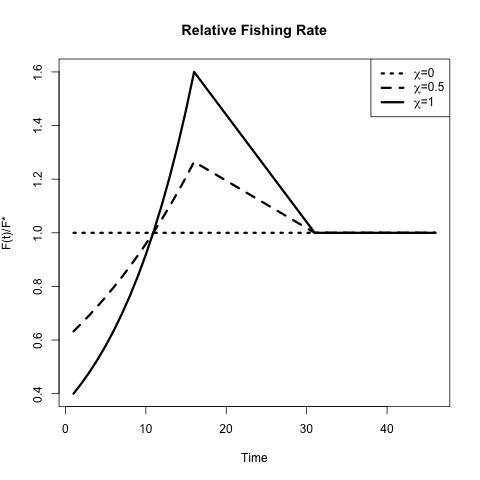
\includegraphics[width=0.44\textwidth]{../ptNew/relFish.png}
%$~$
%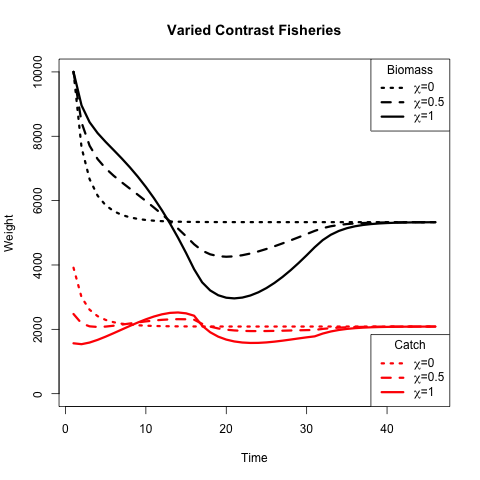
\includegraphics[width=0.44\textwidth]{../ptNew/relSeries.png}
%%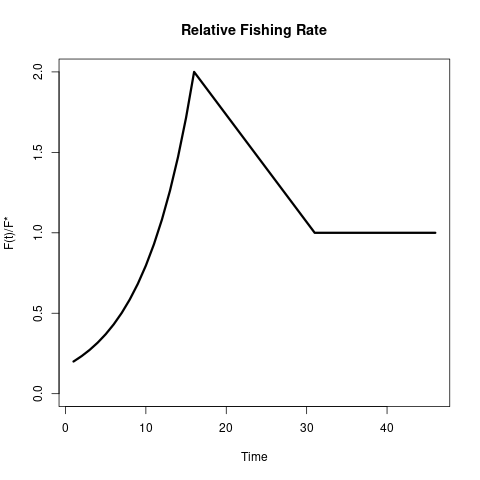
\includegraphics[width=0.45\textwidth]{../../../theses/nick/gpBias/rfExpT45X2Z0.6.png}
%%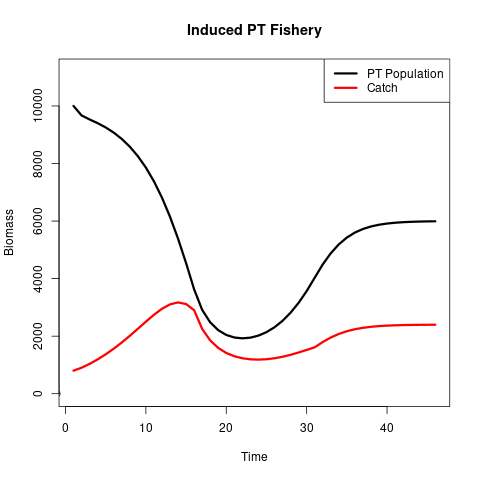
\includegraphics[width=0.45\textwidth]{../../../theses/nick/gpBias/bioCatchExpT45X2Z0.6.png}
%%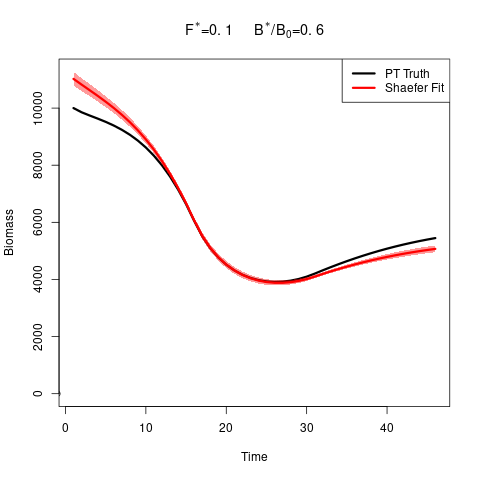
\includegraphics[width=0.5\textwidth]{../../../theses/nick/gpBias/bioPostCompareExpT45X0.5Z0.6.png}
%\vspace{-1cm}
%\caption{ \label{catchT45}
%($left$) Relative fishing with low, medium, and high contrast.
%($right$) Population biomass and catch at each associated level of contrast. %demonstrating contrast in a {\color{red}PT population} with $F^*=0.4$ and $\frac{B^*}{\bar B(0)}=0.6$.
%}
%\label{catch45}
%\end{figure}
%%\clearpage
%%
%When $\chi=0$, the relative fishing rate is a constant at 1 to create a low 
%contrast simulation environment. As $\chi$ increases Eq (\ref{relFish1}) 
%induces more and more contrast in the observed index and catch time series 
%until $\chi=1$ which produces a high contrast simulation environment. 
%Figure (\ref{catch45}) demonstrates a spectrum of contrast simulation 
%environments as well as the time series data they induce in the solution of 
%the production model ODE. 
%
%%%
%%In practice, catch is determined by a series of observed, assumed known, catches. 
%%Catch observations are typically observed on a quarterly (or yearly) basis, so 
%%that the ODE may be discretized via Euler’s method with integration step sizes 
%%to match the observation frequency of the modeled data. In this case, catch is sampled 
%%as would be done in practice however, the simulation can encounter a variety of issues 
%%working with the naively discretized ODE. As a result the ODE is integrated implicitly 
%%via the Livermore Solver \shortcite[lsode]{radhakrishnan_description_1993}, and catch 
%%is linearly interpolated between sampled epochs. 
%%More detail about issues of continuity and ODE integration are described in 
%%Appendix (\ref{appODE}).
%
%%\begin{itemize}
%%	%\item how its parameterized
%%	%\item different behaviors
%%	%\item contrast
%%	\item Forcing function
%%	\item continuity and the solution of ODEs
%%\end{itemize}
%
%%\begin{itemize}
%%	%\item picture relative fishing rate
%%	\item ?quantification of degrees of information? (avg curvature?)
%%	\item remake picture w/o PT references
%%\end{itemize}
%
%%
%%\clearpage
%\subsection{Two Parameter Production Model Inference\label{modelFit}}
%
%%
%The simulated mapping results from fitting an intentionally misspecified two 
%parameter production model to index of abundance data that are generated from 
%a more complex three parameter model of productivity. 
%%The simulation results in an intentionally (and controlled) 
%%misspecified two parameter production model. 
%%The goal of model fitting is to assess how the biological parameters of the
%%two parameter production model behave under MLE inference when index of 
%%abundance data are generated from more complex models of productivity. % three parameter models, to PT data.
%Thus, let $I_t$ be an index of abundance simulated from the three parameter PT 
%or Schnute production models at time $t\in\{1,2, 3,..., T\}$. However the 
%fitted model is specified to be intentionally misspecified so that the fitted 
%model is driven by a two parameter Schaefer, or BH production model respectively. %of productivity. 
%
%%
%The observation model for the fitted model is log-normal such that,
%%
%\begin{align}
%I_t| q, \sigma^2, \bm{\theta} \sim LN(qB_t(\bm{\theta}), \sigma^2).
%\end{align}
%%
%$B_t(\bm{\theta})$ is defined by the solution of the ODEs defined by the Schaefer, or BH models.
%%
%For the Schaefer model $\bm{\theta}=[r, K]$, and for the BH model $\bm{\theta}=[\alpha, \beta]$. 
%%%
%%\begin{align}
%%\frac{dB}{dt} = r B \left(1-\frac{B}{K}\right) - FB. \label{odeS}
%%\end{align}
%%
%From the perspective of the fitted model, the observed $I_t$ are assumed independent 
%conditional on $q$, $\sigma^2$, $r$, $K$ and the two parameter ODE model for biomass. 
%Thus the log likelihood can be written as
%%
%\begin{align}
%\log\mathcal{L}(q, \sigma^2, \bm{\theta}; I) = - \frac{T}{2}\log(\sigma^2) - \frac{1}{2\sigma^2}\sum_t \log\left(\frac{I_t}{qB_t(\bm{\theta})}\right)^2. \label{logLike}
%\end{align}
%
%%
%In this setting, $q$ is fixed at the true value of 0.0005 to focus on the
%inferential effects of model misspecification on biological parameters.
%$\sigma^2$ and $\bm{\theta}$ are reparameterized to the log scale and fit via MLE. 
%%$\sigma^2$ is allowed to be fit to assess overall model fit. 
%Reparameterizing the parameters to the log scale improves the reliability 
%of optimization, in addition to facilitating the use of Hessian information 
%for estimating MLE standard errors.
%%$r$ and $K$ are reparameterized as $log(r)$ and $log(K)$ to improve the regularity of 
%
%%
%Given that the biological parameters enter the likelihood via a nonlinear ODE,
%and further the parameters themselves are related to each other nonlinearly,
%the likelihood function can often be difficult to optimize. A hybrid optimization
%scheme is used to maximize the log likelihood to ensure that a global MLE solution
%is found. The R package GA \shortcite{scrucca_ga_2013, scrucca_extensions_2017} is
%used to run a genetic algorithm to explore parameter space globally.
%Optimization periodically jumps into the L-BFGS-B local optimizer to refine
%optima within a local mode. The scheme functions by searching globally, with the genetic
%algorithm, across many initial values for starting the local gradient-based optimizer. 
%The genetic algorithm serves to iteratively improve hot starts for the local 
%gradient-based optimizer. Additionally, optimization is only considered to be converged
%when the optimum results in an invertible Hessian at the found MLE.
%
%%%
%%{\color{blue}
%%
%%%\ref{appMLE}
%%In Appendix A a profile likelihood method for estimating all of the
%%parameters of the model is derived. The profile likelihood technique greatly
%%improves the reliability of local optimizers when fitting the biological parameters
%%alongside additional nuisance parameters. The catchability parameter $q$ has the
%%effect of rescaling biomass which can often function similarly to the role of the
%%carrying capacity parameter $K$. Thus, the structure of the likelihood may
%%confound $q$ and $K$, and for some data these parameters may only be weakly
%%identifiable. Posing the model in a Bayesian context provides a convenient
%%mechanism for managing these weak identifiability issues. In a tactful Bayesian
%%formulation $q$ and $\sigma^2$ may then be marginalized out of the joint posterior
%%to yield fast and reliable inference \shortcite{walters_calculation_1994}. %deyoreo_integrating_2012}. %deyoreo_integrating_nodate}. %({\color{red} Cite Maria DeYorio pdf}).
%
%
%%{\color{red} $q$ procedure}
%%  
%%%
%%By working with the resulting models parameterized in terms of 
%%$\log(\tilde F^*)$ it tends to improve optimization convergence. Furthermore, 
%%the normality this induces on the log scale, via the Laplace approximation, 
%%yields Log-Normality on $\tilde F^*$, as seen in Appendix {\ref{appA}}. 
%
%
%%}
%
%%
%%\clearpage
%\subsection{Continuous model formulation}
%	%\begin{itemize}
%	%	\item differential equation theory (uniqueness)
%	%	\item chaos
%	%	\item Euler vs. Implicate (e.g. lsoda, etc.)		
%	%\end{itemize}
%
%%
%%\subsection{integrating ODEs, Stiffness, and Interpolation. Oh my!!}
%
%%
%
%%\textit{
%%a preface to regularity issues: identifiability, stiffness, and continuity.
%%}
%
%%\subsubsection{Uniqueness, Continuity, and Identifiability}
%
%%
%An important (and often overlooked) implementation detail is the solution to the
%ODE which defines the progression of biomass through time. % (See Eq(\ref{ode})). 
%As a statistical model it is of paramount importance that this ODE not only have a
%solution, but also that the solution be unique. Of primary concern, uniqueness
%of the ODE solution is necessary for well conditioned inference. %of identifiability of the statistical model.
%
%%
%If the form of $\frac{dB}{dt}$ is at least Lipschitz continuous, then the
%Cauchy-Lipschitz-Picard theorem provides local existence and uniqueness of
%$B(t)$. %, on the condition that the form of $\frac{dB}{dt}$ is at least Lipschitz continuous
%Recall from Eq(\ref{ode}) that $\frac{dB}{dt}$ is separated into
%a term for biomass production, $P(B)$, and a term for removals, $Z(t)B(t)$. 
%For determining Lipschitz continuity of $\frac{dB}{dt}$,
%the smallest Lipschitz constant of $\frac{dB}{dt}$ will be the sum of the
%constants for each of the terms $P(B)$ and $Z(t)B(t)$ separately. Typically any 
%choice of $P(B)$ will be continuously differentiable, which implies Lipschitz 
%continuity. % (since the set of continuous differentiable functions is a subset of the set of Lipschitz continuous functions).
%At a minimum $Z(t)$ typically contains fishing mortality as a function of time 
%$F(t)$ to model catch in time as $C(t)=F(t)B(t)$. $Z(t)$ may or may not contain 
%$M$, but typically $M$ is modeled as stationary in time and does not pose a 
%continuity issue, unlike some potential assumptions for $C(t)$. 
%%However, $Z(t)$ typically models fishing mortality as a function of time which . 
%%(by more strict definition of continuity than Lipschitz continuity, and furthermore cont
%%Thus, the assumed form of $P(B)$ does not typically introduce continuity concerns,
%%unlike some potential assumptions for $Z(t)B(t)$.
%
%%
%In practice $C(t)$ is determined by a series of observed, assumed known, catches. 
%Catch observations are typically observed on a quarterly basis, but
%in practice may not be complete for every quarter (or year) of the modeled 
%period. It is overwhelmingly common to discretize the ODE in time via Euler's 
%method with integration step sizes to match the observation frequency of the 
%modeled data. This is often computationally convenient when the underlying species 
%dynamics are resonably well behaved, however when the dynamics model is used 
%as a statistical model, with the goal of inferring the behavior of the 
%underlying species dynamics, the regularity of the dynamics are not guaranteed. 
%%general evaluating  can present several issues. 
%%strategy often pushes the assumption of catch continuity under the rug. However, 
%An implicit assumption of continuity of catch in time provides the neccessary 
%regularity for the statistical model. Furthermore a continuous handling of the 
%dynamics provides improved accruacy in evaluating the ODE, particually when 
%inferring productivity parameters which largely control the regularity of the 
%dynamics. 
%
%%evaluation of the assumed dynamics as well as improved accruacy in evaluating the assumed dynamics
%%Furthermore 
%%for regularity of the %identifiability of the
%%statistical model an implicit assumption of continuity of the catches is
%%required. 
%%
%%Fish come in different sizes that vary continuously, right? Is there some 
%%argument to be made that continuity is a reasonable approximation because 
%%catch does not involve single fish, but rather a collection of fish with 
%%non-identical weights?
%%
%%While mechanistically at the finest scale fishers must only catch
%%discrete packets of biomass (i.e. individual fish), it is sensible to consider
%%catches as accruing in a continuous way. %at the quarterly (or yearly) scale 
%%Furthermore any assumption of continuity will be required to be at least
%%Lipschitz continuous for the required regularity of the model.
%
%%
%While there are many ways to handle catch continuity, here I assume that catches 
%accrue linearly between observed catches. This assumption defines the catch 
%function as a piecewise linear function of time, with the smallest Lipschitz 
%constant for the catch term defined by the steepest time segment of the catch 
%function. This assumption represents one of the simplest ways of handling catch, 
%while retaining Lipschitz continuity overall. Furthermore linearly interpolated 
%catch is adequately parsimonious for the typical handling of catches.
%
%%
%\subsubsection{Integration and Stiffness}
%
%%
%As previously mentioned, the overwhelming majority of implementations of
%stock assessment models discretized the ODE using Euler's method with the
%integration step sized fixed so as to match the observation frequency. In this
%setting we explore model parameterizations that explore the full extent of
%biologically relevant reference points. This exercise produces some
%combinations of parameters that result in numerically stiff ODEs.
%
%%
%The concept of stiffness in ODEs is hard to precisely characterize.
%%({\color{red}cite}). Hairer and Wanner [5, p. 2] 
%\shortciteA[p.2]{wanner_solving_1996} describe stiffness in the
%following pragmatic sense, ``Stiff equations are problems for which explicit
%methods don't work''. It is hard to make this definition more mathematically
%precise, but this a consistent issue for models of fast growing species in 
%the low contrast simulation. 
%% parameterized
%%so that $\zeta$ is greater than about $\frac{1}{2}$. 
%Euler's method, as often implemented, is particularly poorly suited for these 
%stiff regions of parameter space. In these stiff regions it is necessary to 
%integrate the ODE with an implicit integration method.
%
%%
%Several of the most common implicit methods were tried including the
%Livermore Solver for ODEs (lsode), and the Variable Coefficient ODE Solver
%(vode) as implemented in the deSolve package of R \shortcite{soetaert_solving_2010}. 
%The difference between implicit solvers is negligible, while explicit
%methods result in wildly varying solutions to the ODE in stiff regions of
%parameter space. %explicate methods completely fail to represent the model as
%%stated in the stiff regions of parameter space. 
%Results shown here are computed using the lsode integration %method 
%since it runs relatively quickly and has a relatively smaller footprint in system memory.
%
%%Too stiff for Euler,
%%avoid chaos, and
%%implicit methods
%
%%}

%
%RESULTS
%

%
\clearpage

%
\vspace*{-1.5cm}
\section{Results}

%%
%\subsection{PT/Schaefer}
%
%%
%\subsubsection{An $MSY$-Optimal Catch History \label{flat}}
%
%%
%When $F(t)$ is held constant at $F^*$, as it is in the "low contrast" 
%simulation setting, $B(t)$ comes to equilibrium as an exponential decay from 
%$K$ to $B^*$. Understanding model misspecification bias is simplified in this 
%setting due to the relative simplicity that this induces in $B(t)$. However 
%this simplicity is known to poorly inform estimates of $r$, and thus $F^*$, 
%due to the limited range of the production function that is observed 
%\shortcite{hilborn_quantitative_1992}. 
%%This example is a "low contrast" setting.
%
%%%
%%Figure (\ref{flatProd}) shows four of the most misspecified example Schaefer 
%%function fits as compared to the true data generating PT production
%%functions. In the rug plots below each set of curves the observed biomasses
%%demonstrate the exponential decay from $K$ to $B^*$ in each case. In particular,
%%notice how only biomasses greater than the PT $B^*$ are observed. 
%%Due to the
%%leaning of the true PT curves, and the symmetry of the logistic parabola, the
%%logistic curve only observes information about its slope at the origin from
%%data observed on the right portion of the PT curves. Above the Schaefer line
%%PT is steeper on the right of $B^*$ than it is on the left, and so the the
%%logistic curve over-estimates $r$, and thus $F^*$, for data generated above
%%the Schaefer line. Below the Schaefer line the vice versa phenomena occurs.
%%Below the Schaefer line PT is shallower to the right of $B^*$ than it is on the
%%left and so the logistic parabola estimate tends to under estimate $F^*$.
%
%%\begin{figure}[h!]
%\begin{wrapfigure}{r}{0.5\textwidth}
%\vspace{-0.5cm}
%%\begin{minipage}[h!]{0.49\textwidth}
%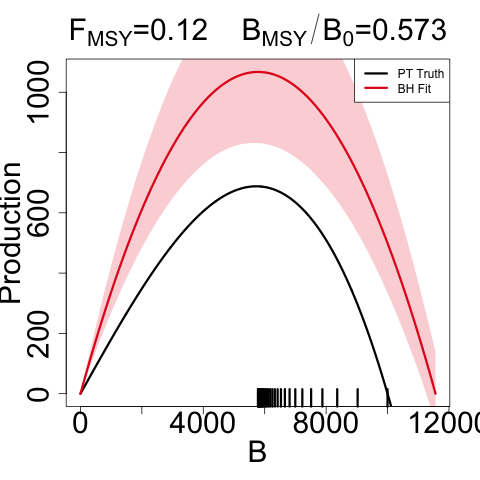
\includegraphics[width=0.24\textwidth]{../ptNew/srrCompareFlatT30X0.12Z0.573.png}
%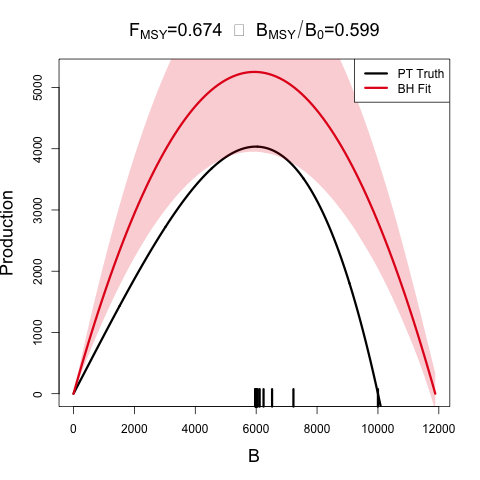
\includegraphics[width=0.24\textwidth]{../ptNew/srrCompareFlatT30X0.674Z0.599.png}\\
%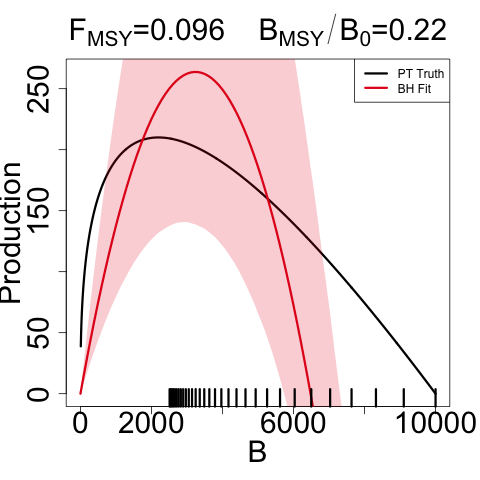
\includegraphics[width=0.24\textwidth]{../ptNew/srrCompareFlatT30X0.096Z0.22.png}
%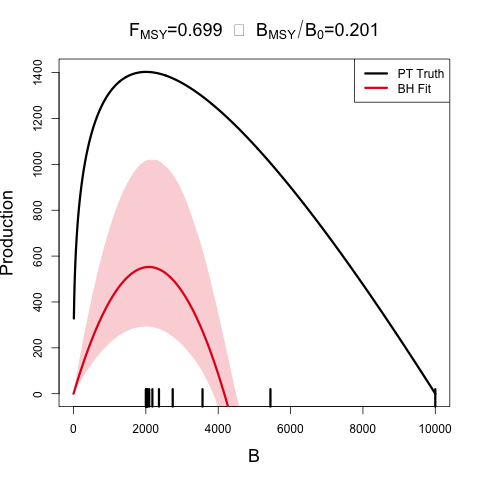
\includegraphics[width=0.24\textwidth]{../ptNew/srrCompareFlatT30X0.699Z0.201.png}
%%\end{minipage}
%%\begin{minipage}[h!]{0.49\textwidth}
%%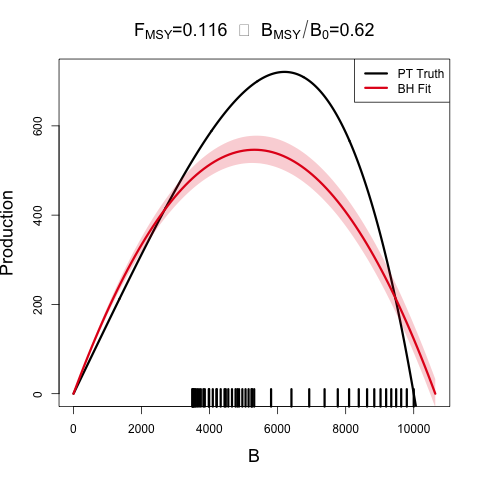
\includegraphics[width=0.45\textwidth]{../ptNew/srrCompareExpT45X0.116Z0.62.png}
%%%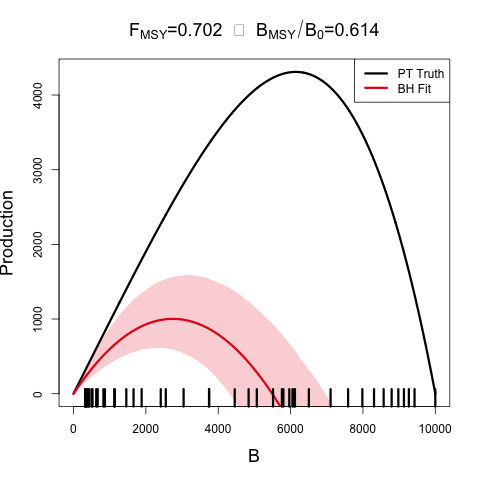
\includegraphics[width=0.45\textwidth]{../ptNew/srrCompareExpT45X0.702Z0.614.png}\\
%%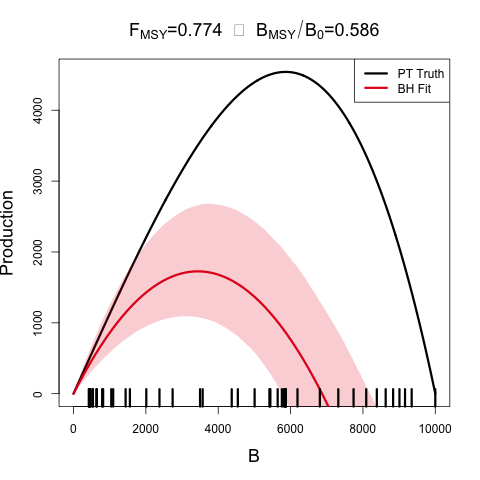
\includegraphics[width=0.45\textwidth]{../ptNew/srrCompareExpT45X0.774Z0.586.png}\\
%%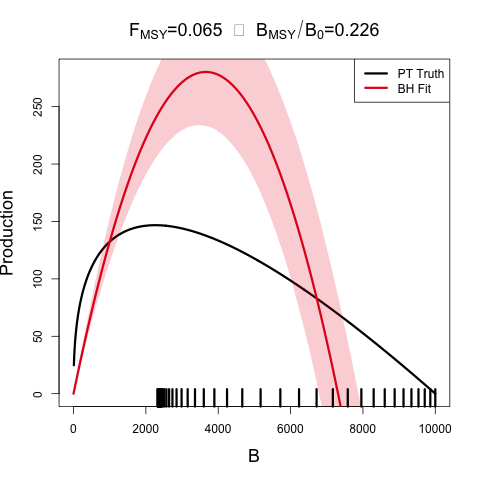
\includegraphics[width=0.45\textwidth]{../ptNew/srrCompareExpT45X0.065Z0.226.png}
%%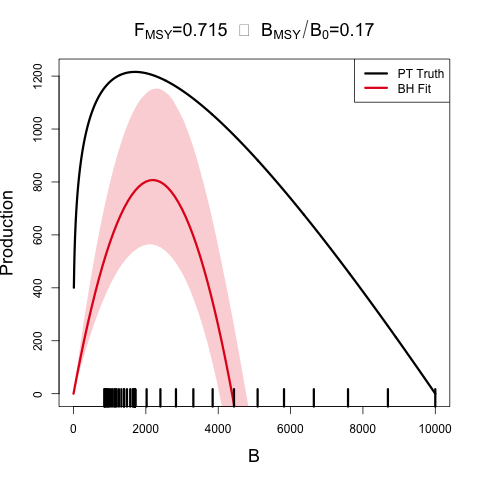
\includegraphics[width=0.45\textwidth]{../ptNew/srrCompareExpT45X0.715Z0.17.png}
%%\end{minipage}
%\caption{
%A comparison of the true PT production function (in black) and the estimated logistic curve (in red)
%with 95\% CI shown. The examples shown represent the four corners of maximum model misspecification
%in the simulated RP-space. Observed biomasses are plotted in the rug plots below the curves.
%%Fitted logistic production function verses true PT production function. 
%%Observed biomass plotted along x-axis.
%}
%\label{flatProd}
%%\end{figure}
%\end{wrapfigure}
%
%%
%Figure (\ref{flatProd}) shows four of the most misspecified example
%production function fits as compared to the true data generating PT production
%functions. The rug plots below each set of curves show how the observed 
%biomasses decay exponentially from $K$ to $B^*$ in each case. In particular,
%notice how observations only exist where the PT biomass is greater than $B^*$.
%Due to the leaning of the true PT curves, and the symmetry of the logistic 
%parabola, the logistic curve only observes information about its slope at the 
%origin from data observed on the right portion of the PT curves. The top two 
%panels of Figure (\ref{flatProd}) shows PT data generated such 
%that $\frac{B^*}{\bar B(0)}>0.5$; in these cases PT is steeper to the right of 
%$B^*$ than it is on the left, and so the the logistic curve over-estimates $r$, 
%and consequently also over-estimates $F^*$. %for data generated above the Schaefer line. 
%The bottom two panels of Figure (\ref{flatProd}) show PT data 
%generated with $\frac{B^*}{\bar B(0)}<0.5$ and where the vice versa phenomena 
%occurs. PT is shallower to the right of $B^*$ than it is on the left and so the 
%logistic parabola estimate tends to under estimate $F^*$.
%
%
%%Below the Schaefer line the vice versa phenomena occurs;
%%Below the Schaefer line 
%%%
%%Figure (\ref{flatProd}) indicates that the individual biases of $B^*$ and $K$
%%may behave quite differently. $B^*$ appears to be estimated fairly accurately
%%while $K$ does not.
%
%
%
%
%
%
%%\begin{itemize}
%%	\item[~] region of chaotic fits due to model misspecification
%%	%\item arrow plots 
%%	\item RP break out plots with mechanism of failure
%%\end{itemize}
%
%%%
%%Figure (\ref{flatTrio}) shows the biases in $F^*$ and $\frac{B^*}{\bar B(0)}$
%%over the space of simulated RPs. The (\emph{top-right}) panel of Figure (\ref{flatTrio})
%%shows how data generated across a broad space of RPs are mapped onto the
%%limited space of the Schaefer line. Below the Schaefer line, RP estimates are
%%biased by over-estimating $\frac{B^*}{\bar B(0)}$ and under-estimating $F^*$.
%%Above the Schaefer line the vice-versa is true; $\frac{B^*}{\bar B(0)}$ is
%%under-estimated and $F^*$ is over-estimated. In the (\emph{left}) and
%%(\emph{bottom}) panels of Figure (\ref{flatTrio}) the bias in $\frac{B^*}{\bar B(0)}$
%%and $F^*$ are shown component-wise; each panel showing the same patterns, but
%%focusing on only one component of the bias at a time. In these panels red
%%coloring indicates over-estimation of the RP and blue indicates under-estimation.
%%Notice that the region of RPs near the Schaefer line enjoy relatively low bias
%%since model misspecification is minor in this region.
%
%%
%\subsubsection{Metamodeled Trends}
%
%%\item define Schaefer line.
%%\item reiterate each point in RP space is an entire PT model, on the Schaefer 
%%line moder are Schaefer.
%
%%
%Each point in the space of the RPs $F^*$ and $\frac{B^*}{\bar B(0)}$ uniquely 
%identifies a complete PT model with different combinations of parameters values. 
%Recall that when $\gamma=2$ for the PT model, the PT curve becomes a parabola 
%and is equivalent to the logistic curve of the Schaefer model. Since the 
%logistic curve is symmetric about $B^*$, the Schaefer model must fix the value of 
%$\frac{B^*}{\bar B(0)}$ at the constant $0.5$ for any value of $F^*$. So 
%the line through RP space defined by $\frac{B^*}{\bar B(0)}=0.5 ~~ \forall ~~ F^*$, 
%defines the subset of RP space where $\gamma=2$ and where the PT model is 
%equivalent to the Schaefer model. For brevity this subset of RP where $\frac{B^*}{\bar B(0)}=0.5$ 
%will be referred to as the ``Schaefer set''. Thus simulated data that are 
%generated along the Schaefer set will be the only data that are not 
%misspecified relative to the Schaefer model; as PT data are simulated 
%farther and farther away from this line at $\frac{B^*}{\bar B(0)}=0.5$ model 
%misspecification of the Schaefer model becomes worse and worse.
%
%%\item generalize the srr figure above
%%\item individual model fits will have jittery trends; metamodel nonlinearly 
%%smooths and pulls information together.
%
%%
%While Figure (\ref{flatProd}) demonstrates a real trend in simulation results, 
%individual simulation runs will at best show jittery trends due to the stochastic 
%nature of statistical inference. The GP process metamodel accounts for this 
%stochasticity %, filters out jitters, %  and allows for the jitters to be filtered out 
%to focus analysis on the signal in the simulation results. Recall that metamodeling 
%occurs on the scale of the inferred productivity parameters of the restricted 
%production model, 
%%by transforming  %(in this case the Schaefer model when fitting PT data. 
%by transforming metamodel predictions via Eq. (\ref{ptRP}), metamodeled predictions 
%are obtained for Schaefer RPs. By further subtracting the true data generating 
%PT RPs from the predicted Schaefer RPs at each point in RP space a pattern of 
%inferential RP bias, induced by model misspecification of the Schaefer model, 
%can be seen. %to be seen. % in Figure (\ref{arrowsPT}).
%
%%using the relevant transformations given in Eq. (\ref{ptRP}) , \ref{BratS}, \ref{FmsyS}) with $\gamma$
%%fixed to the restricting case.
%%
%%Additionally the metamodel generalizes the patterns seen in Figure (\ref{flatProd}) across the entire range of RPs. 
%
%%../ptNew/ptLook.r
%\begin{figure}[h!]
%\begin{minipage}[h!]{0.44\textwidth}
%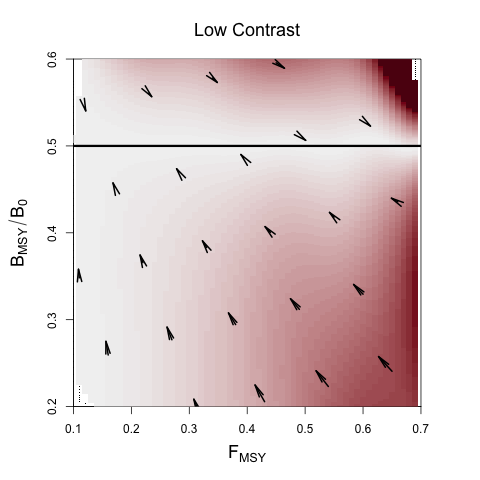
\includegraphics[width=\textwidth]{../ptNew/directionalBiasSubPTFlatT30.png}
%\end{minipage}
%\begin{minipage}[h!]{0.44\textwidth}
%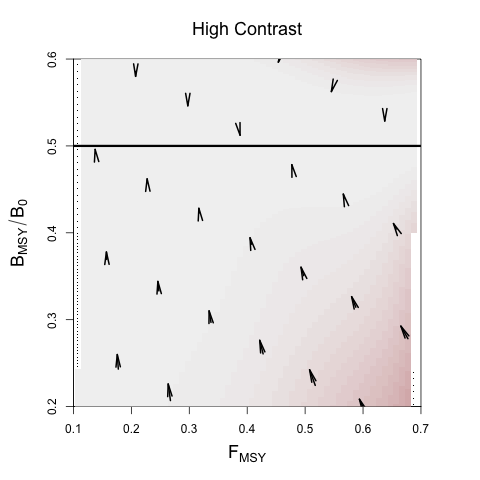
\includegraphics[width=\textwidth]{../ptNew/directionalBiasSubPTExpT45MinCon.png}
%\end{minipage}
%\begin{minipage}[h!]{0.09\textwidth}
%\hspace{-1cm}
%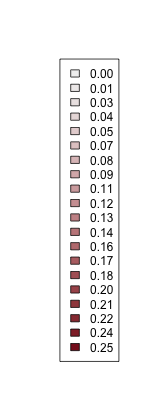
\includegraphics[width=1.5\textwidth]{../ptNew/subLegnd.png}
%\end{minipage}
%\caption{
%Joint bias direction for ($F^*$, $\frac{B^*}{B_0}$) estimates under 
%the misspecified Schaefer Model. The intensity of color represents the excess 
%bias relative to the shortest possible mapping. Results in the low contrast setting 
%are shown $left$, and the high contrast setting is shown $right$.
%}
%\label{arrowsPT}
%\end{figure}
%
%%
%Figure (\ref{arrowsPT}) shows the pattern of biases the Schaefer model creates when fit 
%to PT data generated at each point of RP space. An equivalent way to think of Figure 
%(\ref{arrowsPT}) is that since the Schaefer model must estimate RPs in the Schaefer set, 
%the metamodel arrows indicate the mapping that is created by inferring RPs under 
%a misspecified Schaefer model fit to PT data generated at each point over the pictured 
%region.
%
%%
%Since $\frac{B^*}{B_0}$ must be 0.5 under the Schaefer model, biases in the 
%$\frac{B^*}{B_0}$ direction must simply map vertically onto the Schaefer set.
%Due to this simplified RP geometry under the Schaefer model, the degree of bias in 
%$\frac{B^*}{B_0}$ estimation is defined solely by the degree of model 
%misspecification irrespective of $F^*$. Furthermore, 
%%since the Schaefer line is simply a constant at $\frac{B^*}{B_0}=0.5$, 
%the closest possible point along the Schaefer set that Schaefer model inference %under a Schaefer model 
%could map RPs would be the perfectly vertical mapping. This pattern only contains the 
%strictly necessary bias present in $\frac{B^*}{B_0}$, and zero bias in $F^*$. 
%Any deviation from this minimal bias pattern is necessarily due to added bias in $F^*$.
%
%%
%The two simulation settings shown in Figure (\ref{arrowsPT}) are identical except 
%for the amount of contrast present in the simulated index. The left panel of 
%Figure (\ref{arrowsPT}) shows RP biases in the low contrast setting, while the 
%right panel shows the high contrast setting. Notice that in the low contrast 
%setting the RP bias pattern is far from the minimum distance mapping, however when 
%contrast is added the mapping becomes much closer to a minimal bias mapping. 
%In the low contrast setting the observed bias is consistent with the pattern 
%and mechanism described in Figure (\ref{flatProd}), where $F^*$ is underestimated 
%for data generated below the Schaefer line and overestimated above the Schaefer set.
%In the high contrast simulation the mapping is nearly minimal distance with the exception 
%of PT data generated with simultaneously low $\frac{B^*}{B_0}$ and high $F^*$. 
%
%%
%%\begin{wrapfigure}{r}{0.5\textwidth}
%%\vspace{-0.5cm}
%\begin{figure}
%\begin{minipage}[h!]{0.49\textwidth}
%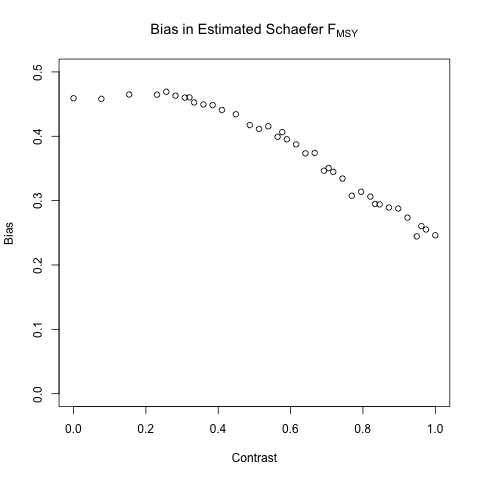
\includegraphics[width=\textwidth]{../ptNew/contrastTest.png}
%\end{minipage}
%\begin{minipage}[h!]{0.49\textwidth}
%\caption{
%Bias in $F^*$ under the Schaefer model when PT data are generated 
%with increasing contrast so that $F^*$ and $\frac{B^*}{B_0}$ are fixed at 
%0.699 and 0.201 respectively. %Bias is shown for the Schaefer models estimation of $F^*$ as a function of contrast.
%%A comparison of the true PT production function (in black) and the estimated logistic curve (in red)
%%with 95\% CI shown. The examples shown represent the four corners of maximum model misspecification
%%in the simulated RP-space. Observed biomasses are plotted in the rug plots below the curves.
%%%Fitted logistic production function verses true PT production function. 
%%%Observed biomass plotted along x-axis.
%}
%\end{minipage}
%\label{conTest}
%\end{figure}
%%\end{wrapfigure}
%
%%
%Figure (\ref{conTest}) demonstrates how bias in $F^*$ estimation %under the Schaefer model 
%decreases as contrast is added to PT data as generated in the low $\frac{B^*}{B_0}$ and 
%high $F^*$ regime. By including additional contrast $F^*$ bias is decreased, however
%parameterizing contrast so as to fully extinguish $F^*$ bias may require a more complex 
%model of fishing.
%%,  in may be By including more contrast $F^*$ bias  in this low $\frac{B^*}{B_0}$, 
%%high $F^*$ region can be further reduce.}
%
%%%
%%\begin{itemize}
%%%\item define Schaefer line.
%%%\item reiterate each point in RP space is an entire PT model, on the Schaefer 
%%%line moder are Schaefer.
%%
%%%\item generalize the srr figure above
%%%\item individual model fits will have jittery trends; metamodel nonlinearly 
%%%smooths and pulls information together.
%%
%%%\item Point out the geometry of Schaefer RPs, thus $\frac{B^*}{B_0}$ must 
%%%simply map vertically. 
%%%\item Bias in $\frac{B^*}{B_0}$ estimation entirely defined by the degree 
%%%of model misspecification.
%%%\item mapping directly vertically is a minimum distance mapping given the 
%%%constrained space.
%%
%%%\item Any biases in $F^*$ moves this mapping further from the mapping with 
%%%minimum possible distance.
%%\item The low contrast simulation indeed demonstrates biased estimation of 
%%$F^*$ as observed in other studies {\color{red}(cite)}. 
%%
%%%%\item adding information (High contrast) reduces $F^*$ bias and thus moves 
%%%%the mapping closer to minimum possible distance.   
%%%\item {\color{orange}bias in $F^*$ at a point in the lower right corner as a function of ``contrast''.}
%%
%%%%At some point
%%%\item summary of $\sigma$ over RP space comparing between models (PT, Schnute, Schnute DD) to show areas of model breakdown.
%%%	\begin{itemize}
%%%	\item miss-identifying signal for noise. 
%%%	\item It happens more as the dynamics get more complex. 
%%%	\item point to the full age structed models.
%%%	\end{itemize}
%%
%%%\item Histogram of high/low contrast $F^*$ bias observations??: I don't think this is necessary unless really pushed by someone
%%\end{itemize}
%
%%\clearpage

%
\subsection{Schnute/BH}

%
\subsubsection{Design}


%
\begin{wrapfigure}{r}{0.45\textwidth}
%\vspace{-3cm}
\vspace{-2cm}
%\begin{figure}[h!]
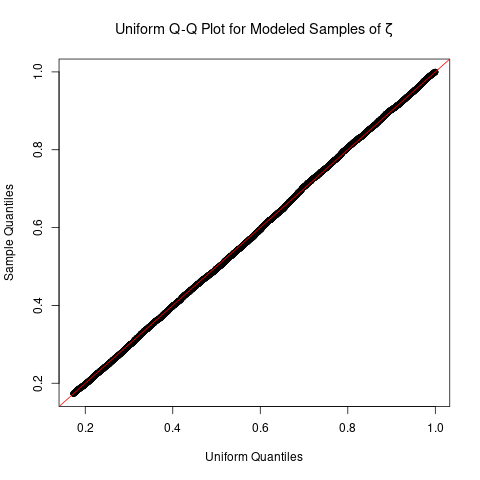
\includegraphics[width=0.45\textwidth]{../gpBias/qqUnif.png}
\vspace{-1cm} %against theoretical uniform quantiles
\caption{Uniform Q-Q plot for $\zeta$ plotted for $F^*=0.1$ and $M=0.2$.}
\label{qqZeta}
%\end{figure}
\end{wrapfigure}

%
Algorithm (1) enforces uniform marginals in $\frac{F^*}{M}$ directly, as well
as the adherence of the overall design to latin squares.  
Figure (\ref{qqZeta}) shows a uniform Q-Q plot for sampled $\zeta$, using 
Algorithm (1), against theoretical uniform quantiles. As evidence by the 
excellent coherence to the theoretical uniform quantiles, the approximation
in Section (\ref{sLHS}) for sampling $\gamma$ (and therefore $\zeta(\gamma$)), 
%for the purpose of computing $\zeta(\gamma$), 
is very effective. 
Furthermore since numerical inversion of $\zeta(\gamma)$ is costly and 
unreliable, the relative speed and accuracy that this approximate LHS sampling 
method provides is pivotal for the rest of the work presented here. %to understanding the relationship between RPs and $\gamma$.

%
%The space filling design generated by Algorithm (1). The space filling algorithm generates
%a uniform marginal in $\frac{B^*}{B_0}$. A uniform marginal in $\frac{F^*}{M}$ can 
%be enforced directly. %Algorithm (1) also ensures that the resulting design respects a latin 
%square. 

%The only apprixmate result is in the uniformity of the $\frac{B^*}{B_0}$ 
%marginal which is excellent.

%
\begin{wrapfigure}{r}{0.5\textwidth}
\vspace{-0.5cm}
%\begin{figure}[h!]
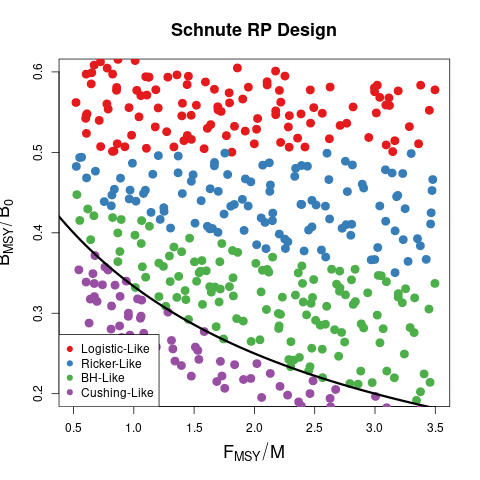
\includegraphics[width=0.5\textwidth]{../gpBias/designLineColorHHardFlatT30N150WWideN112.png}
%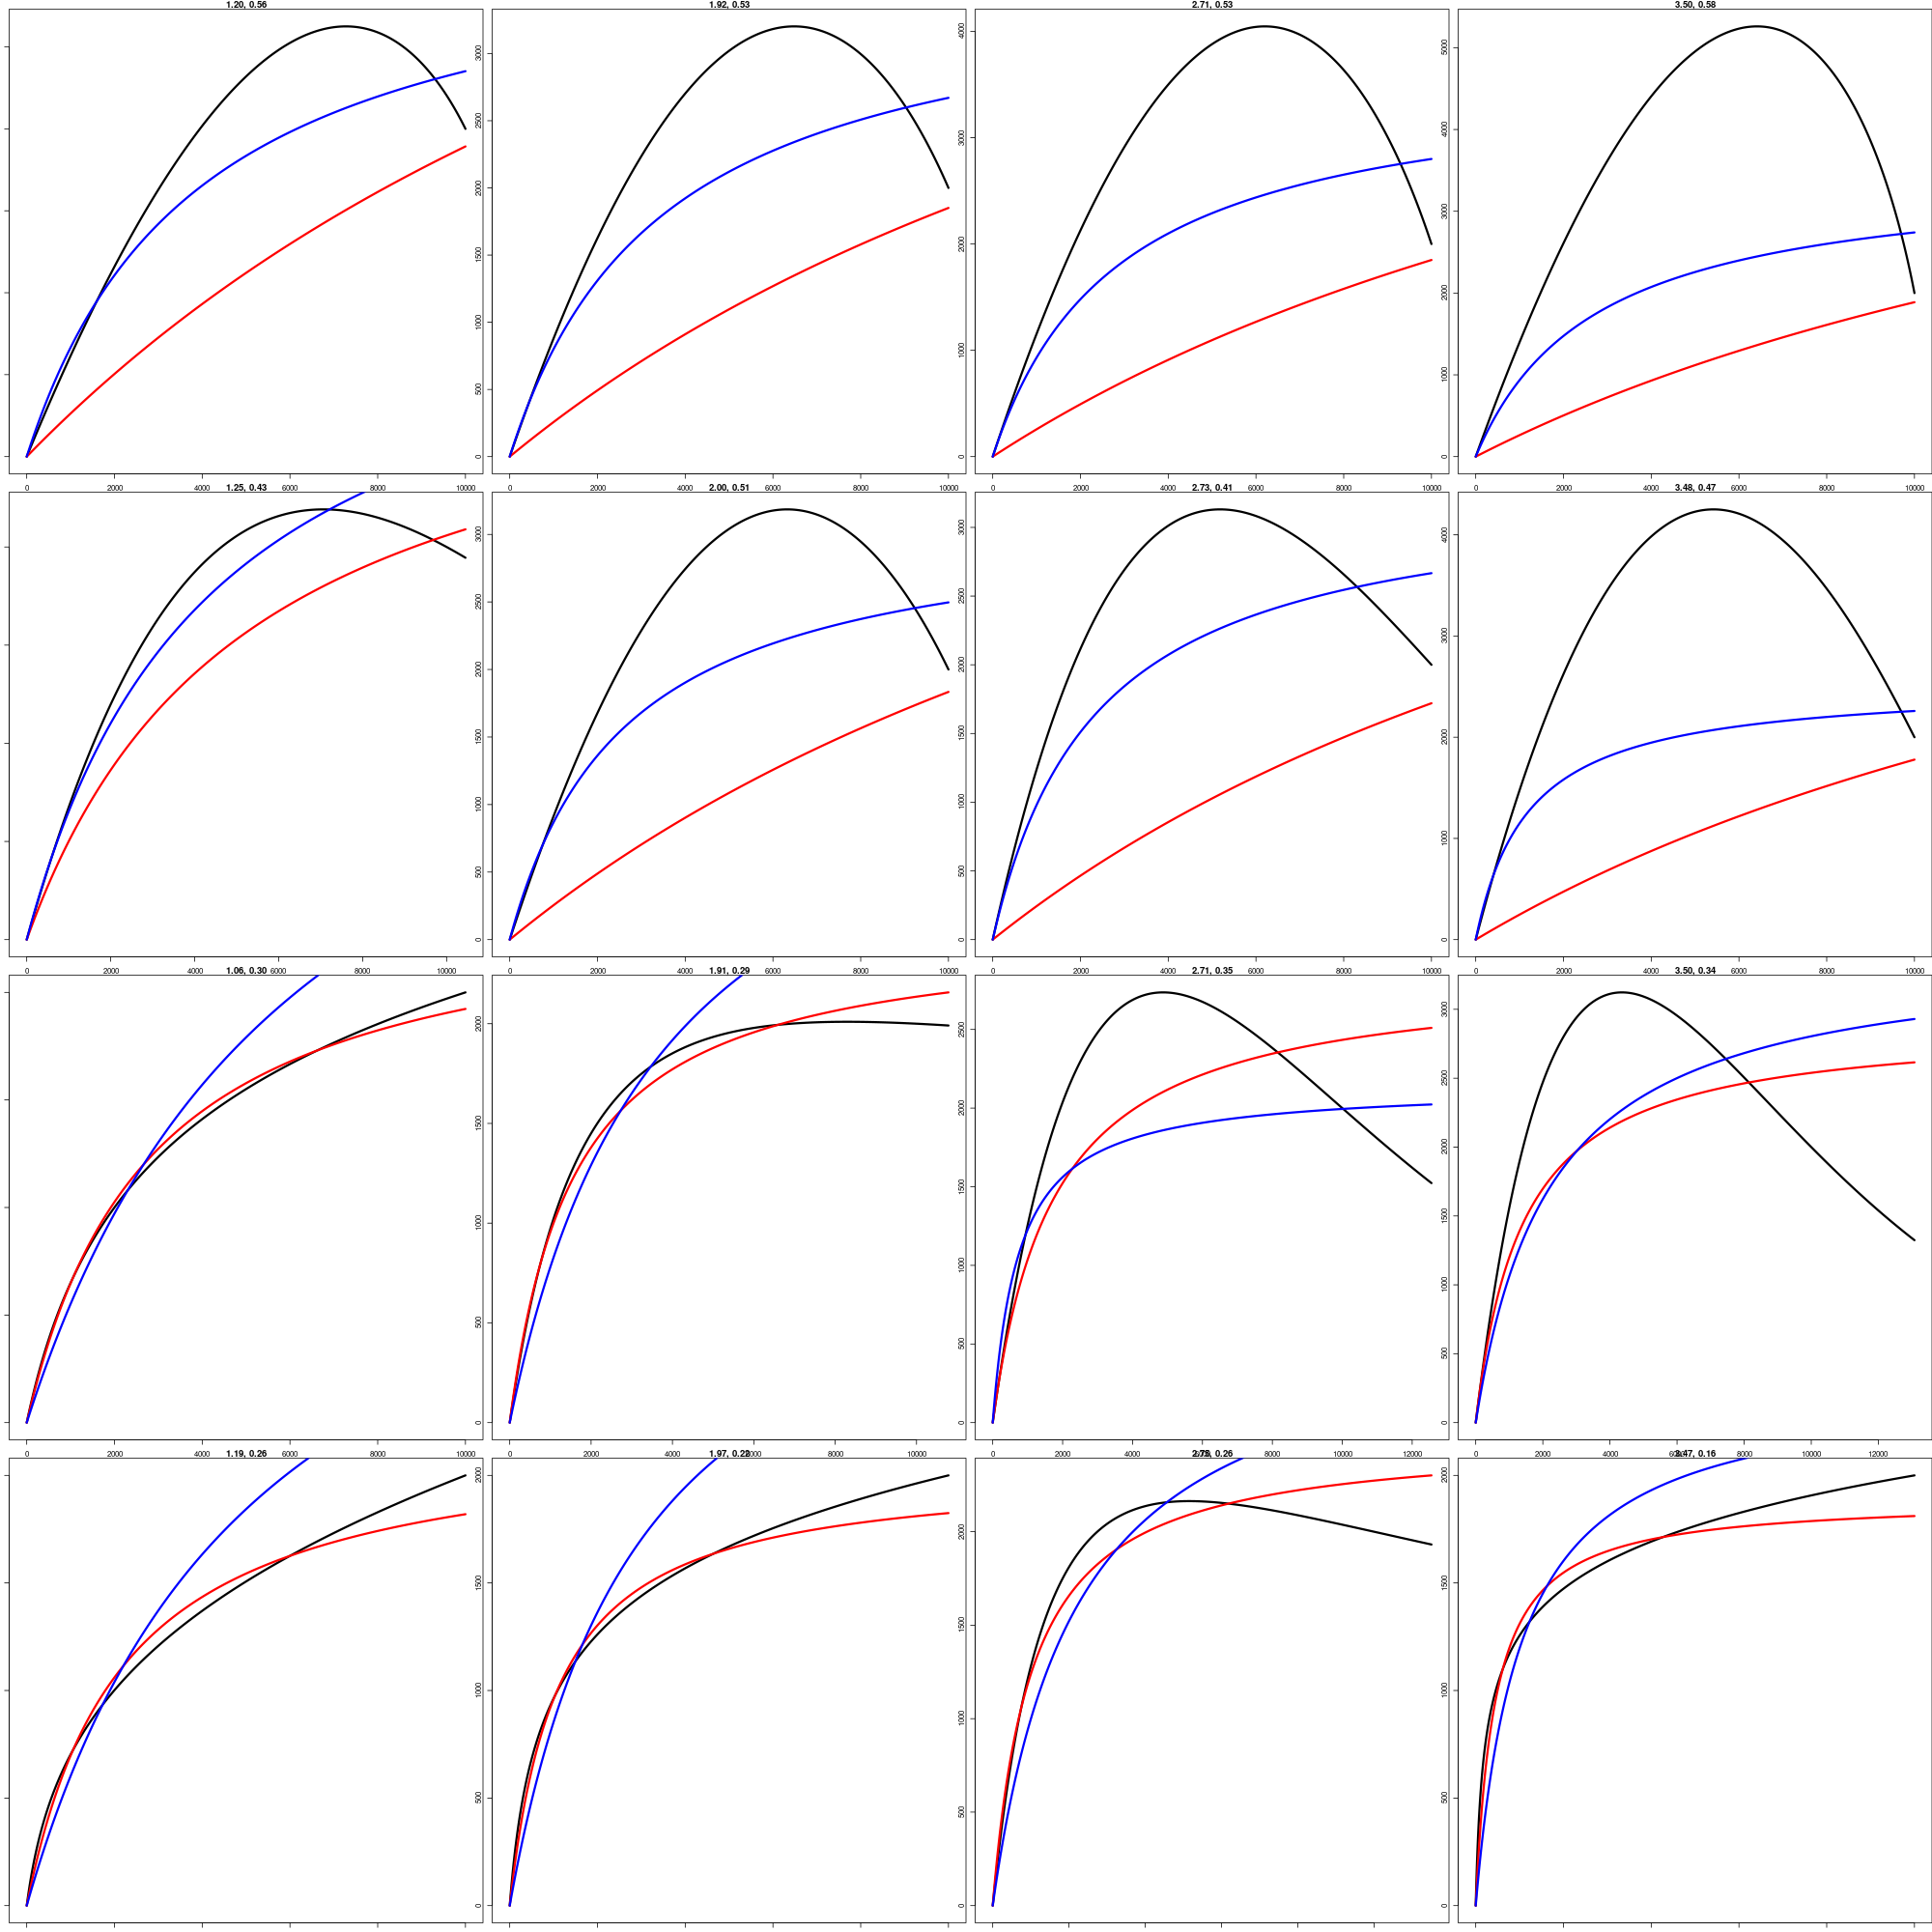
\includegraphics[width=0.5\textwidth]{../gpBias/rGridHHardFlatT30N150WWideN112.png}
\vspace{-1cm}
\caption{
A Schnute RP design. % resulting from design refinement of Algorithm (1). 
Colors indicate different regimes of Schnute production. % function.
%Samples are colored by the ranges the $\gamma$ parameter which result in 
%different regimes of the Schnute production function.
The black curve shows the BH set.
}
\label{colorDes}
%\end{figure}
\end{wrapfigure}

%
Similarly to the PT model, the three parameter Schnute model is uniquely 
identified by each point in the space of $\frac{F^*}{M}$ 
and $\frac{B^*}{B_0}$ RPs. As seen in Figure (\ref{colorDes}), Schnute 
production has different behaviors in different ranges of RPs space, which 
are entirely defined by the value of $\gamma$ (shown in Figure (\ref{sRegimes})). 
%As shown in Figure (\ref{sRegimes}), as well as the colors of Figure (\ref{colorDes}), 
When $\gamma\ge1$ the Schnute model produces a family of Logistic-like curves that are 
increasingly right leaning as $\gamma$ increases. 
For $1>\gamma\ge0$, Schnute production takes a family of left leaning Ricker-like curves 
that all, at least, approach the x-axis. For $0>\gamma>-1$ there are a family of BH-like 
curves that do not approach the x-axis but still have decreasing productivity for large
biomass stocks. When $\gamma$ is exactly $-1$ Schnute reduces to BH production which has 
asymptoting production for large biomass. Finally when $-1>\gamma$ Schnute 
produces a family of increasing Cushing-like curves that do not asymptote, and produces 
linear production as $\gamma\to-\infty$.

%
%Under BH production the full theoretical space of 
%RPs are limited to the curve $\frac{B^*}{B_0}=\frac{1}{F^*/M+2}$.
%Again, for brevity define the BH set as the set of RPs defined by this limited space, 
%i.e. the curve $\left\{\left(\frac{B^*}{B_0}, \frac{F^*}{M}\right) \;\middle|\; \frac{B^*}{B_0}=\frac{1}{F^*/M+2}\right\}$.
%The farther away from this set that Schnute data are simulated, the worse the 
%BH model is misspecified for those data. 
%
%
%\begin{itemize}
%\item demonstrate that my space filling design does in fact result in a uniform $\frac{B^*}{B_0}$ margin.
%\item Show a dense design.
%\item comment on how different regions of the Schnute behave differently. 
%\item compare to Figure (\ref{sRegimes})
%\item 
%\end{itemize}

%
Modeling index data that are simulated broadly over the theoretical space of RPs 
with misspecified BH production greatly limits the range of possible RPs that 
can be inferred. Under BH production the full theoretical space of RPs are 
limited to the curve \mbox{$\frac{B^*}{B_0}=\frac{1}{F^*/M+2}$.} Define the 
``BH set'' as the set of RPs defined by this limited space, i.e. the curve \\
$\left\{\left(\frac{F^*}{M}, \frac{B^*}{B_0}\right) \;\middle|\; \frac{B^*}{B_0}=\frac{1}{F^*/M+2}\right\}$.
as seen in the black curve in Figure (\ref{colorDes}).
The farther away from this set that Schnute data are simulated, the worse the 
BH model is misspecified for those data. 


%
\subsubsection{Metamodeled Trends}


%
Unlike the Schaefer model, the BH set is not a constant in 
$\frac{B^*}{B_0}$. Under the BH model, bias in $\frac{B^*}{B_0}$ is no 
longer entirely defined by the degree of model misspecification, but rather the 
structure of BH RPs allows bias in both $\frac{B^*}{B_0}$ and $\frac{F^*}{M}$ 
to interact as a function of contrast in the data.
%This has the effect of allowing the bias in $\frac{B^*}{B_0}$ and $F^*$ 

%%
%While metamodeling occurs on the inferred productivity parameters of the 
%restricted production model, the metamodel can also be used to build 
%estimates of major biological RPs. For the BH model the relevant 
%transformations for relating productivity parameters with RPs are given in 
%Eqs. (\ref{BratS}, \ref{FmsyS}) with $\gamma$ fixed to -1. 
%%reference points.
%
%%estimate of two productivity parameters under the restricted production model. Each of the fitted productivity parameter
%%estimates are then modeled using independent instances of the following model in Eq (28).
%
%%
%Applying the metamodel predictive surfaces on the scale of RP estimates allows for the 
%quantification of RP bias. % induced by fitting a misspecified BH model 
%%ication of two parameter production functions. 
%%Below 
%RP bias is quantified by the following relative measure of bias, similar to a percent error calculation.
%%
%\begin{align}
%\text{Relative Bias} = \frac{\hat{RP}-RP}{RP}
%\end{align}
%%
%Above $RP$ is a stand-in for the true value of any of the biological
%reference points under the three parameter data generating production model, 
%and $\hat{RP}$ refers to the metamodel estimate of each RP quantity under the 
%BH model. %two parameter restricted cases.

%
\begin{figure}[h!]
\begin{minipage}[h!]{0.49\textwidth}
\hspace*{-0.5cm}
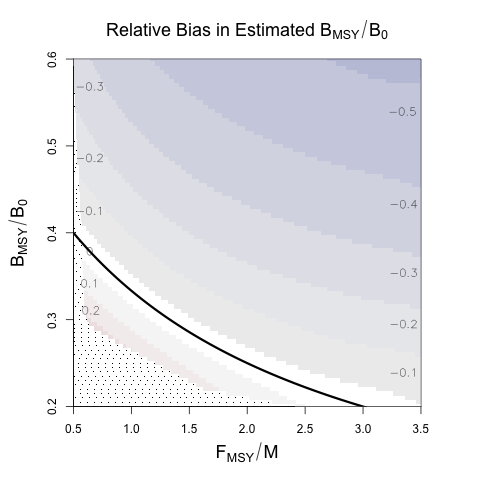
\includegraphics[width=1.1\textwidth]{../gpBias/zetaRelBiasSchnuteExpT45N150Wide.png}\\
%\hspace*{1cm}
\caption{\label{contrastTrio}
Heatplots showing the bias in RP estimation induced by model misspecification of 
the BH model in the high contrast simulation setting. 
In all cases the restricted RP-space of the BH set is shown as the black curve.  
(\emph{left}) Relative bias in $\frac{B^*}{\bar B(0)}$.  (\emph{top-right}) 
Bias in RP-space shown directionally. Arrows point from the location where 
data is generated, toward the location in the BH set where MLE projects estimated 
RPs. The intensity of color represents the excess bias relative
to the shortest possible mapping. (\emph{bottom}) Relative bias in $F^*$.  
}
$~$\\$~$\\
\end{minipage} 
\begin{minipage}[h!]{0.49\textwidth} 
\hspace*{1cm}
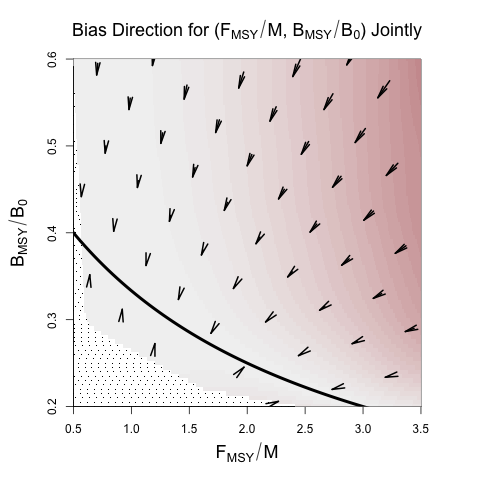
\includegraphics[width=1.1\textwidth]{../gpBias/directionalBiasSchnuteSubTitleExpT45N150Wide.png}\\
\hspace*{1cm}
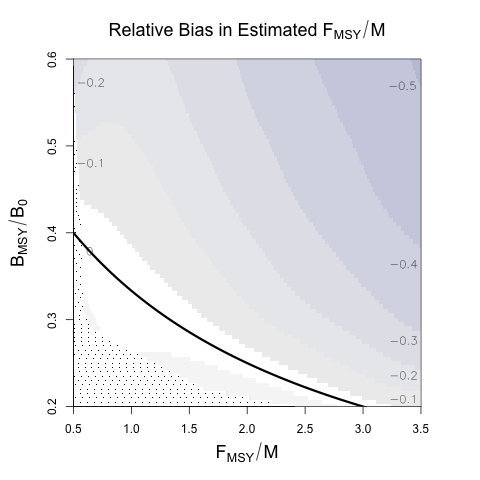
\includegraphics[width=1.1\textwidth]{../gpBias/fMSYRelBiasSchnuteExpT45N150Wide.png}
\end{minipage}
\end{figure}

%
\paragraph{High Contrast}

%
Figure (\ref{contrastTrio}) shows metamodeled RP bias surfaces for inference 
under the BH model in the high contrast setting. The (\emph{left}) and 
(\emph{bottom}) panels focus only on the $\frac{B^*}{\bar B(0)}$ and 
$\frac{F^*}{M}$ components of bias respectively. In these panels bias is shown
as relative bias, $\frac{\widehat{RP}-RP}{RP}$, similar to a percent error calculation.
Where $RP$ represents the true value of the three parameter RP, and $\widehat{RP}$ 
refers to the metamodel estimate.

%
Figure (\ref{contrastTrio}, \emph{top-right}) combines the components of bias to 
show the overall mapping of RPs under BH inference in the high contrast 
simulation setting. Unlike high contrast RP inference under the Schaefer model, 
the BH model does shows bias in both RPs here. Despite the bias in 
$\frac{B^*}{\bar B(0)}$ and $\frac{F^*}{M}$ these results are similar to 
that of the Schaefer model in that the overall mapping of RPs is very nearly a 
minimal distance mapping onto the constrained set of RPs. %In this setting the 
The primary difference between Schaefer model and BH RP inference is the geometry of 
their limited RP spaces. Unlike the Schaefer model the BH set encourages
bias in both RPs for misspecified models even in very well informed setting.

%Above $RP$ is a stand-in for the true value of any of the biological
%reference points under the three parameter data generating production model,
%and $\hat{RP}$ refers to the metamodel estimate of each RP quantity under the
%two parameter restricted cases.
%
%
%
%%In the high contrast simulation setting 
%Unlike the The Schaefer model both RP plays
%By considering 

%\begin{itemize}
%\item Bias present in high contrast $\frac{F^*}{M}$.
%\item While bias is present in $F^*$ the BH mapping is similar to the Schaefer simulation in that the overall mapping
%is very near a minimal distance mapping in RP space.
%\item bias present in $\frac{F^*}{M}$
%\end{itemize}

\paragraph{Low Contrast}

%
\begin{wrapfigure}{r}{0.5\textwidth}
\vspace{-0.5cm}
%%\vspace{-1.25cm}
%\begin{figure}[h!]
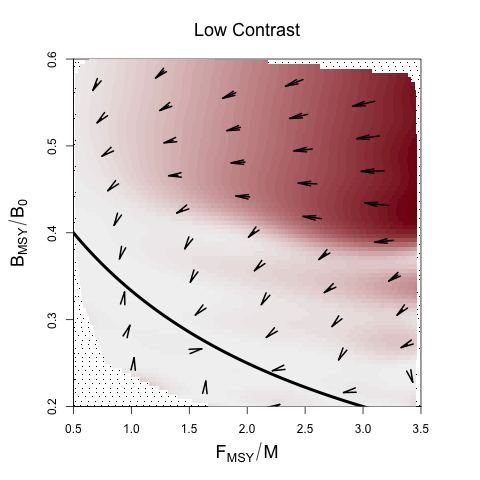
\includegraphics[width=0.5\textwidth]{../gpBias/directionalBiasSchnuteSubHHardFlatT30N150WWideN112.png}
%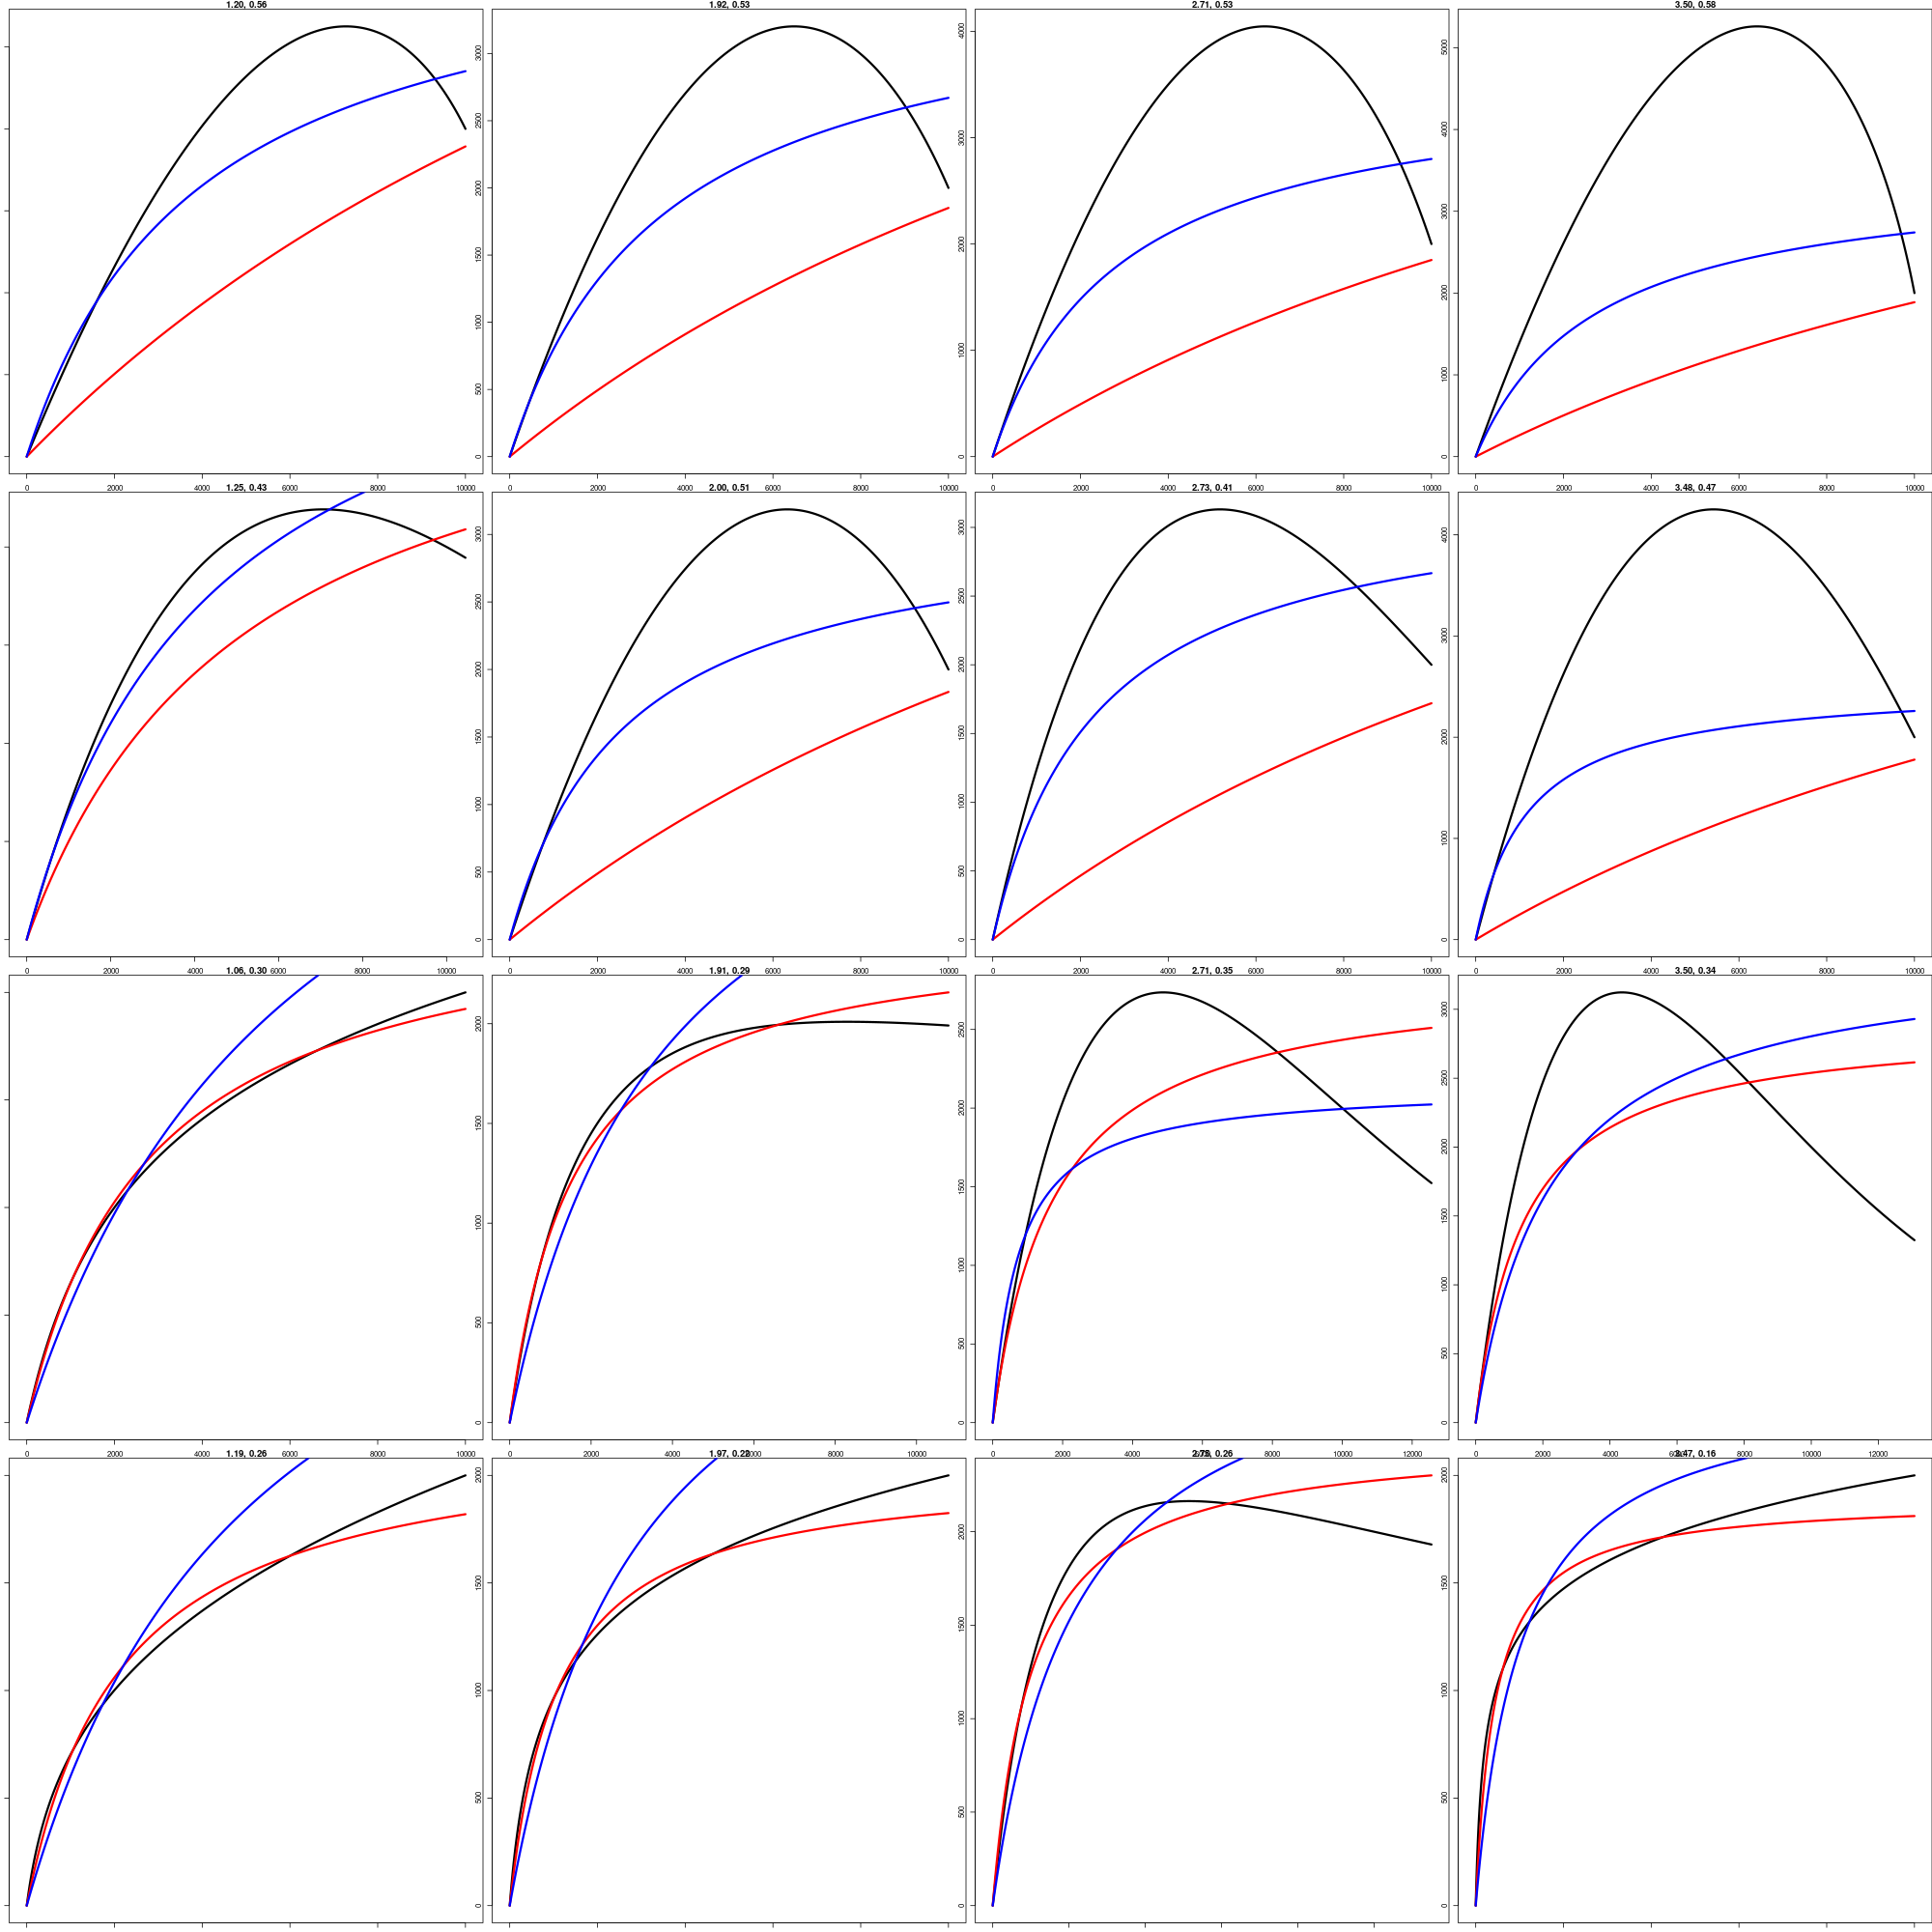
\includegraphics[width=0.5\textwidth]{../gpBias/rGridHHardFlatT30N150WWideN112.png}
\vspace{-1cm}
\caption{
%Relative bias in $F^*$ in the high contrast simulation setting. The BH set is also shown in black. 
Joint bias direction of RP inference in the low contrast simulation setting.
The intensity of color represents the excess bias relative
to the shortest possible mapping. 
}
\label{bhLowArrows}
%\end{figure}
\end{wrapfigure}

%
Figure (\ref{bhLowArrows}) shows the mapping of RPs in the low contrast 
simulation setting. Figures (\ref{bhLowArrows}) and (\ref{contrastTrio}, 
\emph{top-right}) share a common scale for the intensity of color to 
facilitate comparison. In Figure (\ref{bhLowArrows}) notice that the mildly 
misspecified area around the BH set produces mappings onto the BH set which 
resemble the minimal distance mapping seen in the high contrast setting. % %in Figure (\ref{contrastTrio}, \emph{top-right}). %
The primary difference in this low contrast setting, is the break point 
around $\frac{B^*}{\bar B(0)}=0.4$ above which $\frac{F^*}{M}$ is sharply 
underestimated. 

%
The region of RPs where the BH model manages to recover the minimal distance 
mapping may be considered a ``safe regime'' of data types that are 
reasonably well modeled by a BH model. By comparison of Figure (\ref{bhLowArrows}), 
with Figure (\ref{colorDes}), this safe regime of the BH model occurs for data 
generated for Cushing-like or BH-like production. While bias of the RPs can still become concerningly large, % here, %(as large as $X$ in the worst case) within this region, 
this region can be considered safe in the sense that even for low contrast data 
RP estimation under the the BH model recovers the minimal distance mapping.

%
\begin{wrapfigure}{r}{0.5\textwidth}
\vspace{-0.75cm}
%\begin{figure}[h!]
%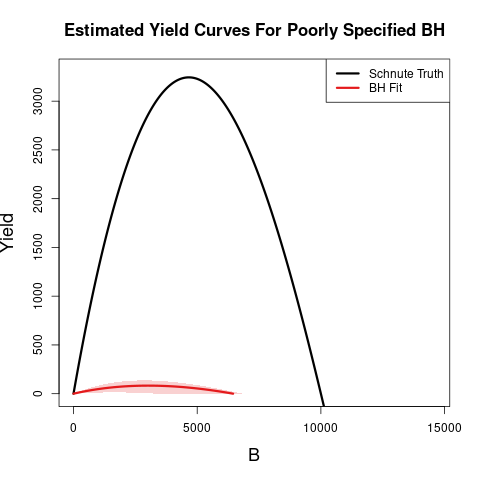
\includegraphics[width=0.5\textwidth]{../gpBias/yeildCurveCompareHHardFlatT30N150WWideN112PrettyX3.4791Z0.4662.png}
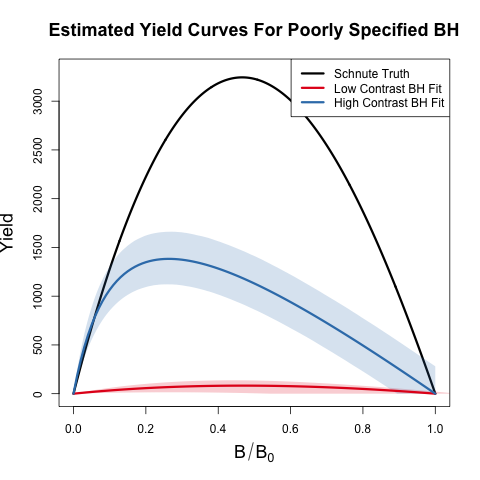
\includegraphics[width=0.5\textwidth]{../gpBias/yeildRelCurveCompareHHardFlatT30N150WWideN112PrettyX3.4791Z0.4662.png}
%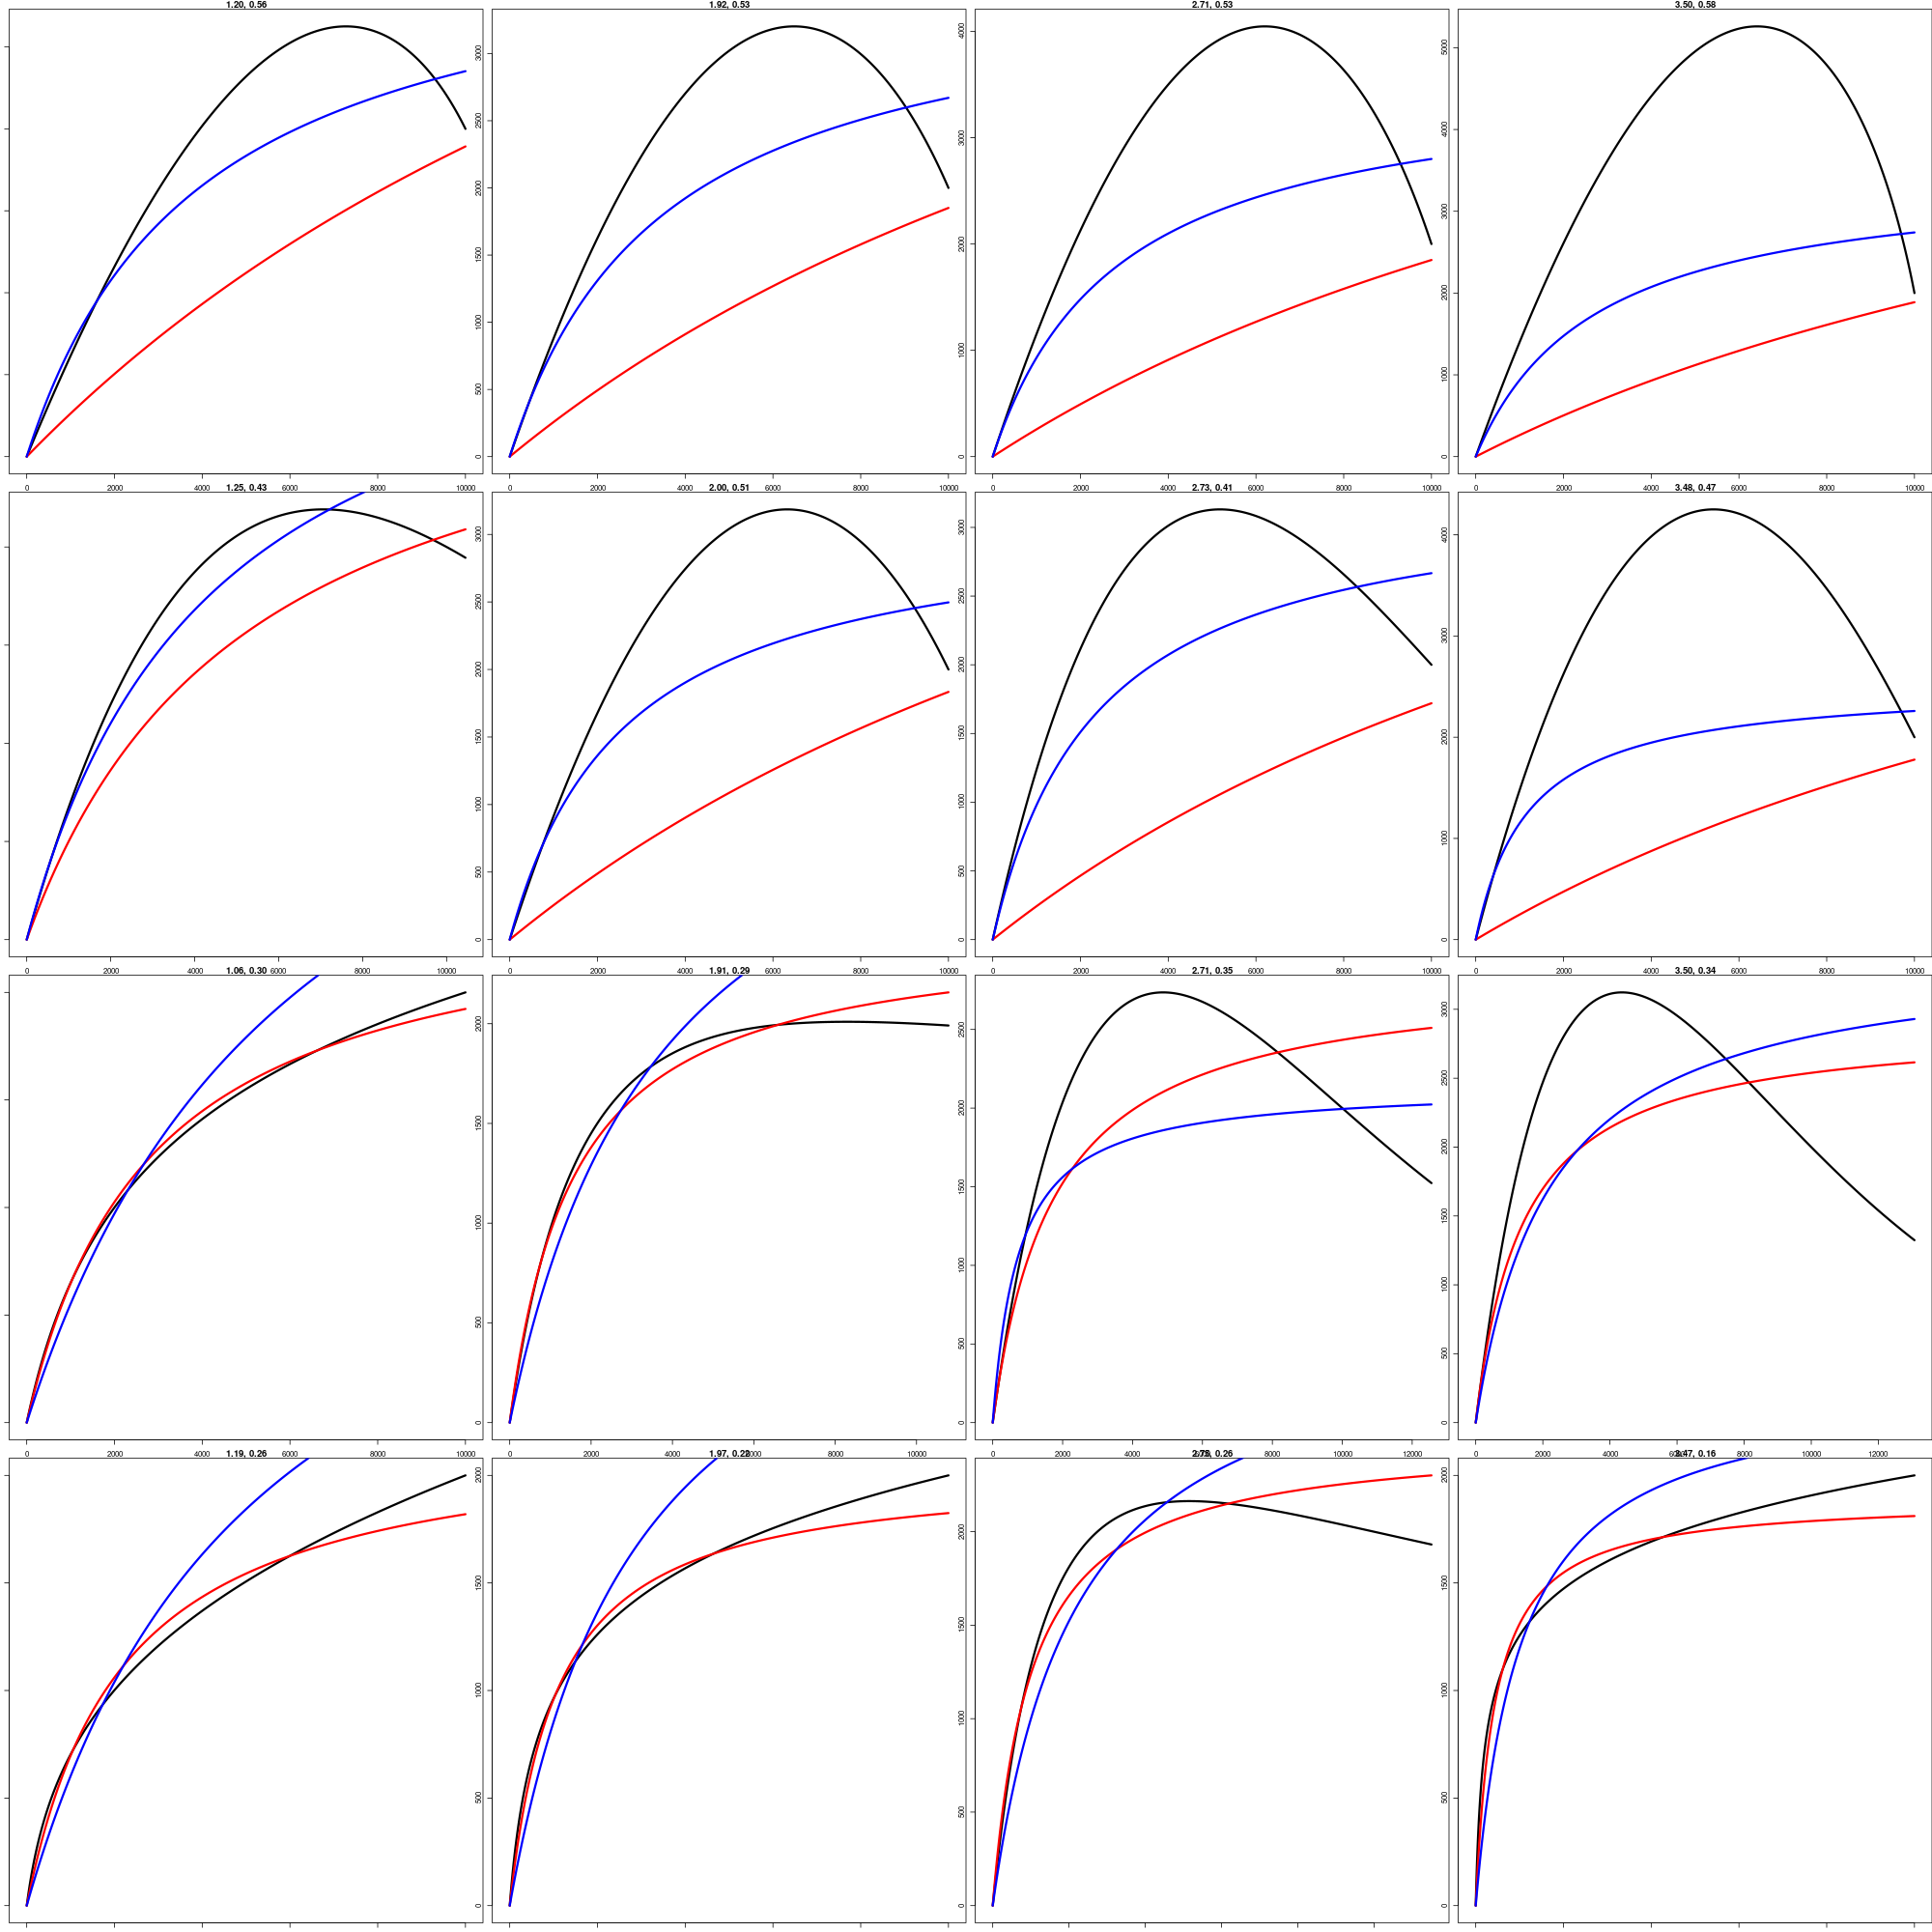
\includegraphics[width=0.5\textwidth]{../gpBias/rGridHHardFlatT30N150WWideN112.png}
\vspace{-1cm}
\caption{
Yield curves for data generated with $\frac{F^*}{M}=3.48$ and $\frac{B^*}{\bar B(0)}=0.48$. 
%Convert into $B/B_0$. Show the high contrast curve.
}
\label{bhFmsy}
%\end{figure}
\end{wrapfigure}

%
Outside of this safe regime, RP estimation breaks from the minimal distance mapping 
at the interface between BH-Like and Ricker-Like regimes of the Schnute model (again see 
Figure (\ref{colorDes})). The Ricker model lies along this regime interface, and  
represents the first model to approach the x-axis for large biomasses as $\gamma$ 
increases. This markedly unBH-like productivity in the low information simulation 
setting breaks MLE inference from the minimal distance mapping and instead maps
RPs to extremely low values of $F^*$; consequently $\frac{B^*}{\bar B(0)}$ 
is estimated near the limiting value under the BH (i.e. $\lim_{F^* \to 0}\frac{1}{F^*/M+2}=0.5$).
Similarly the set of Ricker RPs (as well as the Schaeffer set) include this 
trivial limiting point in common ($\frac{F^*}{M}=0$, $\frac{B^*}{\bar B(0)}=0.5$). 

%
Interestingly, in the high contrast setting this trivial mapping for highly 
misspecified BH models is not present. This suggests that, under a 
misspecified BH model, the presence of adequate information in the data to 
produce reasonable estimates of $\frac{F^*}{M}$, drives $\frac{B^*}{\bar B(0)}$ 
below $0.5$ in accordance with $\frac{B^*}{\bar B(0)}=\frac{1}{F^*/M+2}$, 
even when the true $\frac{B^*}{\bar B(0)}>0.5$. 
%This suggests that in the presence of adequate 
%information in the data to produce reasonable estimates of $\frac{F^*}{M}$ 
%drives $\frac{B^*}{\bar B(0)}$ away from 0.5, even when the true $\frac{B^*}{\bar B(0)}>0.5$. 
This phenomena balances RP estimation within the constrained BH set as 
mediated by the information content of the data and the degree of model 
misspecification. When the information content in the data is too small to 
drive a compromised RP estimate, inference completely disregards accurate 
estimation of $F^*$ in order to better estimate $\frac{B^*}{\bar B(0)}$ 
by exploiting the common limiting behavior of the BH set and that of 
Ricker-like and Logistic-like models. 
%may fail by completely disregarding one RP so the sake of preserving whatever 
%similarities may exist between the functional forms of the data and misspecified model. 

% Similarly 
%information driving $\frac{B^*}{\bar B(0)}$

%
%This suggests that in the absence of information
%and a large degree of model misspecification 
%
%Ignoring $F^*$ to 
%focus on $\frac{B^*}{\bar B(0)}$
%
%BH set converges with Ricker set and Schaeffer set at the trivial point $(0, 0.5)$.
%Outside of the safe regime inference in the absence of informative information. BH inference maps to 
%this common member of the Schaeffer-Like, Ricker-Like and BH-Like regimes. 
%This is represents catastrophic inferential failure.
%
%
%low information content
%data 




%By comparison of Figure (\ref{bhLowArrows}), with the location 
%of the BH-Like and Ricker-Like regimes seen in Figure (\ref{colorDes}), this 
%break point coincides with the threshold between the BH-Like and Ricker-Like 
%regimes of the data generating Schnute model. The Ricker model lies along 
%this regime interface, representing the first model to approach the x-axis for 
%large biomasses as $\gamma$ increases. 
%
%%
%As evidence by this break point, in the low contrast simulation setting, the approach the x-axis for 
%large biomasses
%
%However, even in the low contrast setting the BH model manages to recover the 
%minimal distance mapping for data generated under the Cushing-like or BH-like 
%regimes. These regimes may be considered a sort of ``safe regime'' of data types 
%that are reasonably well modeled by a BH model. 
%
%Even still within this safe regime bias in RP can be as high as $X$ percent. That said 
%the sense in which these regimes are safe is that the RP mapping resemble the 
%minimal distance mapping. geometry of BH mixed RP biases.  
%
%    
%
%
%
%
%
%
%\clearpage
%\begin{itemize}
%%\item introduce BH set
%%\item reiterate each point in RP space is an entire Schnute model, on the BH set modes are BH.
%
%%\item Point out the geometry of BH RPs
%%\item under BH Bias in $\frac{B^*}{B_0}$ is no longer entirely defined entirely by the degree of model misspecification.
%%(still largely)
%%
%%\item Best case data result in a minimum distance mapping (discussion?)
%%\item Due to the shape of the BH RP set this ensures bias in both $\frac{B^*}{B_0}$ and $F^*$
%%\item Unlike the Schaefer models geometry the BH set has a geometry that will mix bias directions in the best case.
%%
%%\item some detail views in $B^*$, $B_0$, $F^*$, $?F_{SPR?}$, $MSY$
%%\item ``safe'' regime similar to the high contrast minimal distance mapping for mild model misspecification.
%%\item Ricker-like break point. Complete model failure beyond.
%%\item what is going on with SRR when model completely fails.
%%%\item mapping directly vertically is a minimum distance mapping given the 
%%%constrained space.
%%\item Mechanism plot on SRR LHS Grid plot
%
%\item mapping distance as a function of contrast at (3.5, 0.5)
%
%\item for LHS grid locations show $\frac{B^*}{B_0}$ and $F^*$ biases for grids in $M\in(0,0.5)$ For sure in High Contrast, maybe also in Low??.
%
%\end{itemize}
%
%
%%../gpBias/animFigSchnuteLHS.r 
%\begin{figure}[h!]
%%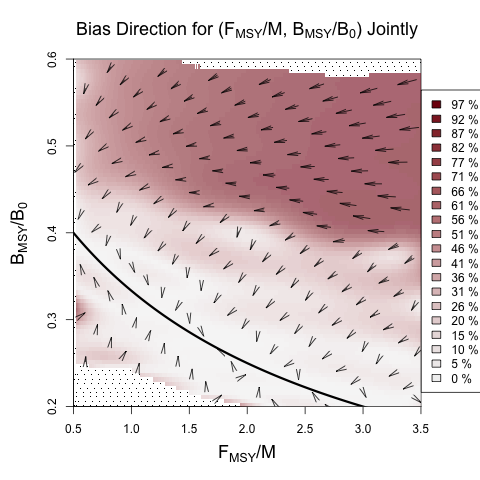
\includegraphics[width=0.5\textwidth]{../gpBias/directionalBiasSchnuteAnimatePrecentHHardFlatT30N150WWideN56X3Z0.35.png}
%\begin{minipage}[h!]{0.44\textwidth}
%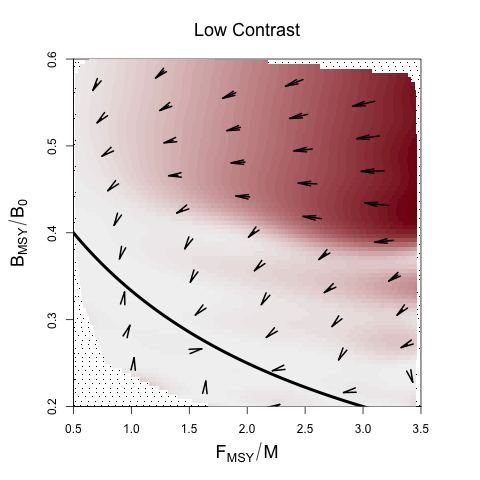
\includegraphics[width=\textwidth]{../gpBias/directionalBiasSchnuteSubHHardFlatT30N150WWideN112.png}
%\end{minipage}
%\begin{minipage}[h!]{0.44\textwidth}
%%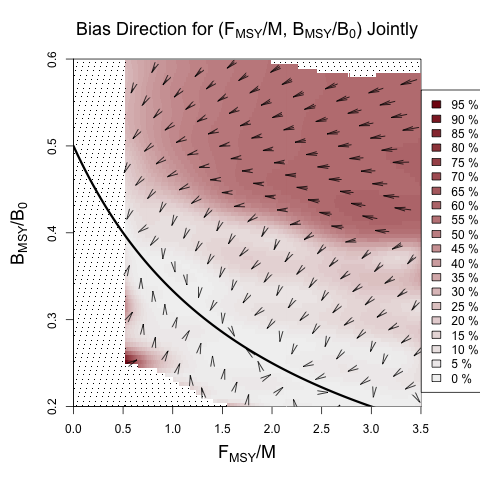
\includegraphics[width=0.5\textwidth]{../gpBias/directionalBiasSchnuteAnimatePrecentHHardFlatT30N150WWideN112X3Z0.55.png}
%%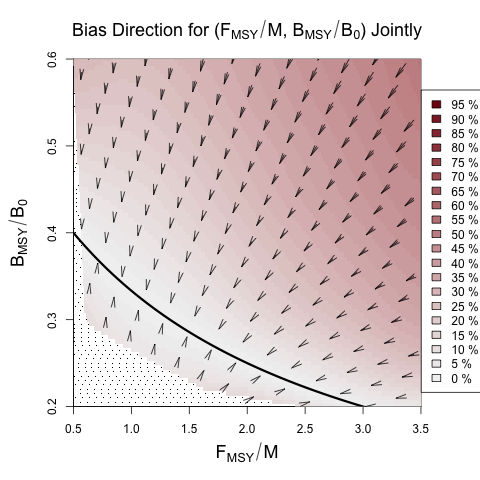
\includegraphics[width=0.5\textwidth]{../gpBias/directionalBiasSchnuteAnimatePrecentExpT45N150WideX3Z0.35.png}
%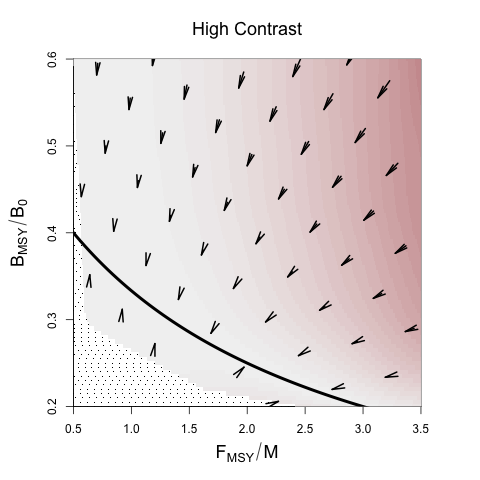
\includegraphics[width=\textwidth]{../gpBias/directionalBiasSchnuteSubExpT45N150Wide.png}
%%\hspace*{-1cm}
%\end{minipage}
%\begin{minipage}[h!]{0.09\textwidth}
%\hspace{-1cm}
%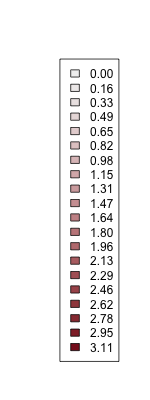
\includegraphics[width=1.5\textwidth]{../gpBias/legendSubSchnute.png}
%\end{minipage}
%\caption{Joint bias direction of RP inference in the low contrast simulation setting.
%%for $\left(\frac{F^*}{M}\right.$, $\left.\frac{B^*}{B_0}\right)$ 
%%estimates under the misspecified BH Model. 
%The intensity of color represents the excess bias relative 
%to the shortest possible mapping. 
%%The high contrast relative fishing setting is 
%%shown $right$; the low contrast setting is shown on the $left$.
%}
%%\caption{\color{red} Low Contrast/High Contrast Titles, unify the Legends (Only show one.) Redo the colors relative to minimum distance. Less arrows. Bolder arrows, bolder line}
%%\label{bhLowArrows}
%\end{figure}
%
%%Figure (\ref{bhLowArrows}) shows the mapping of RPs in the low contrast simulation setting.
%
%%the high contrast setting. Unlike RP inference under the Schaefer model, in the high 
%%contrast setting the BH model does show  
%%
%%Similar to RP inference under the Schaefer model, RP 
%%inferred under a misspecified BH 
%%describe contrast setting.

%
\section{Discussion}

%;
%the simulation design and metamodeling methods presented here further generalize these
%results of these existing results.
%Existing

%
Results presented here generally agree with what is known about estimating
growth rate parameters \shortcite{lee_can_2012, conn_when_2010, magnusson_what_2007}.
These study's appreciate the role of contrast for estimating growth rates, 
however they struggle to make generally extensible conclusions since they focus only 
on a handful of stocks that fall short of forming a random sample of the greater 
population of possible stock behaviors. The LHS design methods presented here are 
designed specifically to simulate a representative sample of stocks broadly 
across the space of possible RPs. Furthermore, the simulation design, taken together 
with the GP metamodel of productivity parmater estimates, allows this study to control 
the degree of model misspecification and generalize conclusions about the behavior 
of productivity estimation within the production model setting presented. 

%%
%Unfortunately, we are unable to generalize the relationship because the twelve 
%assessment examples are not a random sample from the population of all fish 
%stocks and sample size is small. A more general conclusion may be obtained by 
%including more assessments
%%
%\begin{itemize}
%\item \shortcite{lee_can_2012} Generalizability via random sample of fisheries, LHS RP explicitly does this.
%\item multiple starting locations and convergence defined as positive definite Hessian.
%\end{itemize}

%
In the presence of contrast, $F^*$ estimation can enjoy very low bias even
for a wide range of poorly specified models; conversely in the absence of contrast
$F^*$ estimation can suffer very large bias even for slightly misspecified models.
This pattern is particularly true for inference under the Schaefer model where the 
geometry of the restricted RP set isolates estimation failure of $F^*$ from 
$\frac{B^*}{\bar B(0)}$. While contrast has a similar impact on $F^*$ estimation 
under the BH model, the geometry of the BH RP set correlates estimation bias 
of $F^*$ and $\frac{B^*}{\bar B(0)}$. The GP metamodeling approach reveals a 
more general pattern that highly informative data sets (high contrast) 
produces a nearly minimal distance mapping of RPs %that are nearly minimal distance mapping 
onto the constrained RP set.

%
In all cases when model misspecification is removed, even with weakly informative 
data, RP estimation is unbiased and well estimated. Thus contrast alone is 
not the only factor leading to inferential failure. Model misspecification is a 
necessary but not sufficient condition for inducing RP estimation bias. The 
particular RP bias present depends on the RP geometry of the fitted model and 
how that geometry is misspecified relative to the data. The RP mapping is then oriented 
to the RP geometry of the fitted model. 

%
%NOTE: BITCH ABOUT NOT BEING ABLE TO PRODUCE A PERFECTLY INFORMATIVE TIME SERIES
%SPECULATE ABOUT IDEALLY INFORMATION CATCH PATTERNS (DYNAMIC CALIBRATION OF $F^*$)
While the relative fishing rate parameterized in Section (\ref{catch}) captures a usefully 
broad spectrum of relevant fishing behaviors, it is still limiting in the amount of information 
that it can induce. Improved methods for quantifying contrast in fisheries data, and/or methods of 
discovering more informative fishing behavior, could improve this analysis. In the absence of a %Without knowing a 
maximally informative dataset simulation methods will not fully describe how 
inference fails, but the methods presented here tell the most complete picture 
yet, with explicit control of the degree model misspecification, contrast, and 
a simulation design that allows for uniform representative data generation 
across biologically meaningful stocks. The results presented here suggest the 
conjecture that under a maximally informative dataset, RP inference with a two 
parameter production function will be biased in the direction a shortest distance 
map from the true RPs onto restricted set of RPs under the two parameter model.    

%
Given the potential for model misspecification of RPs, a minimal distance 
mapping of RPs represents a best-case scenario where the total bias of RPs, 
when measured jointly, is minimized. That said, without recognizing the 
geometry of how two parameter models of productivity limit RP space this may 
lead to unintuitive implications in RP estimation. For example, due to the 
shape of the BH RP set a minimal distance mapping ensures that if there is 
bias in one of $\frac{B^*}{B_0}$ or $F^*$, there will necessarily be 
bias in the other RP. However under the Schaefer model, since the RP set is a 
constant in $\frac{B^*}{B_0}$, bias in $F^*$ is not adulterated in the 
same way by bias in $\frac{B^*}{B_0}$ estimation. While models with 
constant RPs, such as the logistic model $\frac{B^*}{B_0}=\frac{1}{2}$ or 
the Fox model $\frac{B^*}{B_0}=\frac{1}{e}$, are extremely limited, they 
can be valuable tools for developing intuition precisely because they isolate 
RP estimation in their free RPs from the correlated RP biases present in 
models like the BH or Ricker model. 

%
When one considers the implications of RP bias, overestimation of RPs carries 
the severe implication of management recommendations potentially leading to 
overfishing, while underestimation of RP leads to overly conservative management.
In this sense, when the true model is not known, the geometry of the BH set together 
with the metamodeled bias trends makes the BH model a naturally conservative 
estimator of RPs for most stocks. For most non-BH populations the BH model is 
likely to make conservative errors in its estimates of $F^*$ and $\frac{B^*}{B_0}$. 
The one notable exception to the conservatism of the BH model stands for data 
generated in the Cushing-like regime of Schnute RPs. In this regime the BH 
model tends to be fairly unbiased overall, however the bias that is present 
for these populations tends to be overestimation in both RPs, leading to much 
more severe management consequences for those populations.

%
The RP bias trends of the Schaefer model demonstrate much less conservatism than the BH overall.
For any population with $\frac{B^*}{B_0}<0.5$, $\frac{B^*}{B_0}$ will be overestimated. 
When the population comes from the regime where $\frac{B^*}{B_0}>0.5$, $\frac{B^*}{B_0}$ 
will be under estimated, but $F^*$ is likely to be overestimated depending on the degree of 
contrast present in the data. So while the Schaefer model is an intuitive model, it tends to 
lead to much less conservative RP estimation. 

%
While it is important to recognize these limitations of two parameter models 
of productivity, we should not solely accept conservativism as a rational of 
choosing a BH model of productivity. %Ultimately accuracy of RP estimation, 
%without structural RP biases, %and accurate assessment of uncertainty is a better state 
Increasing the flexibility of the production function by moving toward 
three parameter models would release the underlying structural limitations 
\shortcite{mangel_perspective_2013} that cause these RP biases in the first place. 
\shortciteA{punt_extending_2019} %(Mangel et al., 2013). Punt and Cope (2019) 
considers a suite of possible three parameter curves which could be used 
instead of current two parameter curves. For all of their benefits, three 
parameter production functions have their own complicating factors, and the 
structure present in the Schnute model explored here makes it an intuitive bridge 
model for developing three parameter models going forward.



%In practice, when the true model is not known and the Schaefer model is unlikely to be correctly specified


%inference is oriented to the shape of the constrained space
%conjecture that with perfectly informed models mapping would be orthogonal
\begin{itemize}
%\item model misspecification story as in advancement
	%\begin{itemize}
	%	%\item Results presented here generally agree with what is known about estimating 
	%	%growth rate parameters \shortcite{lee_can_2012, conn_when_2010, magnusson_what_2007}.
	%	%\item These study's appreciate that role of contrast for estimating growth rates, 
	%	%however do not explicately control the degree of model misspecification relative to RPs. 
	%	
	%	%\item In the presence of contrast $F^*$ estimation can enjoy very low bias even 
	%	%for a wide range of poorly specified models; conversely in the absence of contrast 
	%	%$F^*$ estimation can suffer very large bias even for slightly misspecified models. 
	%	
	%	%\item In all cases when model misspecification is removed, even with weakly 
	%	%informative data, $F^*$ estimation is unbiased.  
	%	%\item Model misspecification is thus a necessary but not sufficient condition for inducing bias. 
	%	%\item Behavior of bias is mediate by contrast.

	%\end{itemize}

%\item inference is oriented to the shape of the constrained space
%\item conjecture that with perfectly informed models mapping would be orthogonal
%%NOTE: BITCH ABOUT NOT BEING ABLE TO PRODUCE A PERFECTLY INFORMATIVE TIME SERIES
%%SPECULATE ABOUT IDEALLY INFORMATION CATCH PATTERNS (DYNAMIC CALIBRATION OF $F^*$)
%
%\item Best case data result in a minimum distance mapping (discussion?)
%\item Due to the shape of the BH RP set this ensures bias in both $\frac{B^*}{B_0}$ and $F^*$
%\item Unlike the Schaefer models geometry the BH set has a geometry that will mix bias directions in the best case.

%\item The geometry of the BH set largely encourages underestimation of RPs
%\item The only exception in this simulation is for cushing-like data where the BH tends to slightly overestimate RPs, but 
%largely recovers accurate RP estimates even in the low contrast (low information) simulation (inferential) setting.
%\item Assuming BH for all species is likely a conservative assumption for most species (especially when $F^*$ is high).
%\item however it presents a warped view of management and likely leaves money on the table for species with high $F^*$.
%
%\item Schaefer model underestimates $F^*$ when the true $\frac{B^*}{\bar B(0)}<\frac{1}{2}$, %originate below the Schaefer line 
%and overestimates $F^*$ when the true $\frac{B^*}{\bar B(0)}>\frac{1}{2}$. % true RPs originate below the Sc
%\item This is of particular note since these outcomes carry such varied real would implications. 
%\item Overestimation of $F^*$ carries the severe implication of management 
%recommendations potentially leading to overfishing, while underestimation of $F^*$ leads to overly conservative management. 

\item {\color{blue}show a schnute fit to data? \shortcite{yeakel_generalized_2015} Prior} % and how it fixes issues.}
%\item logistic/fox model triangulation (bias correction).

\end{itemize}

%\section{Discussion\label{dis}}
%
%%
%Results presented here generally agree with what is known about estimating 
%growth rate parameters \shortcite{lee_can_2012, conn_when_2010, magnusson_what_2007}, 
%in this case $r$, and thus $F^*$.  
%%These study's appreciate that role of contrast for estimating growth rates, 
%%however do not explicately control the degree of model misspecification 
%%relative to RPs.  %present over as wide a range of RPs and how bias 
%In the presence of contrast $F^*$ estimation can enjoy very low bias even 
%for a wide range of poorly specified models; conversely in the absence of 
%contrast $F^*$ estimation can suffer very large bias even for slightly 
%misspecified models. In all cases when model misspecification is removed, even 
%with weakly informative data, $F^*$ estimation is unbiased.  Model 
%misspecification is thus a necessary but not sufficient condition for inducing 
%bias. 
%
%%{\color{red} 
%%Claim novelty. meta modeling to integrate factors of bias location, direction, magnitude considered along catch.  
%%}
%
%%%
%%The metamodeling approach presented here indicates that the Schaefer model 
%%underestimates $F^*$ when the true $\frac{B^*}{\bar B(0)}<\frac{1}{2}$, %originate below the Schaefer line 
%%and overestimates $F^*$ when the true $\frac{B^*}{\bar B(0)}>\frac{1}{2}$. % true RPs originate below the Schaefer line. 
%%This is of particular note since these outcomes carry such varied real would 
%%implications. Overestimation of $F^*$ carries the severe implication of 
%%management recommendations potentially leading to overfishing, while 
%%underestimation of $F^*$ leads to overly conservative management.   
%
%%considered jointly
%While it is established that growth rate parameters require contrast to estimate, 
%the implications of these biases jointly across a variety of RPs have not 
%received as much attention. 
%%In particular the joint analysis of RP estimation that this 
%%metamodeling approach allows 
%%has not been studied. 
%When considering $B^*$ alongside $F^*$ in varying contrast environments, it 
%becomes clear that different data informs different parts of the production 
%function differently. In low contrast environments $B^*$ is estimation is 
%remarkably unbiased across all but the most challenging instances of model 
%misspecification. However in the presence of contrast, while $F^*$ enjoys 
%better estimation, $B^*$ estimation experiences substantial bias for only 
%modestly misspecified models. Further, by augmenting contrasting data with an 
%additional period of low contrast data this pattern begins to reverse with $B^*$ 
%bias receding toward more poorly specified models and $F^*$ bias encroaching 
%toward only modestly misspecified models as seen in Figure (\ref{expT90BmFm}).   
%
%%
%The behavior of bias in estimating $B^*$ and $F^*$ suggests that the limited 
%parameter space of the Schaefer model induces a trade off in estimating these 
%parameters. In practice, when the true model is not known and the Schaefer 
%model is unlikely to be correctly specified, one should at best expect to only 
%estimate either $B^*$ or $F^*$ correctly depending on the particular degree of 
%model misspecification. The observed contrast then serves to distribute the 
%available information among $B^*$ and $F^*$. Increasing the flexibility of the 
%production function by moving toward curves with additional parameters could 
%release these structural limitations \shortcite{mangel_perspective_2013}. 
%\shortciteA{punt_extending_2019} considers a suite of possible three parameter
%curves which could be used instead of current two parameter curves.
%
%%
%This study only explores the compatibility of the possible productivity shapes 
%exhibited by the PT and Schaefer models. While the PT and Schaefer models are 
%instructive for a variety of dome shaped production behaviors, %non-compensatory production behaviors, 
%it is possible that under different modeling assumptions, for example %compensatory 
%BH production or age structured models, different bias patterns 
%will emerge. Extending this work to be able to make claims in those settings 
%is necessary for developing more generally extensible claims. % and my proposal for this extension can be seen in Section(\ref{})
%
%%
%Given the role that catch plays in understanding where the production function 
%is informed, it is clear that good estimates of catch are important for 
%contextualizing modeling inferences. While the production model treats catches 
%as known without uncertainty, upon inspection of Figure (\ref{hakeData}, \emph{right})
%this assumption is clearly suspect. Results presented here only consider very 
%deterministic catch histories. More work is needed to understand how jittery catch may 
%affect RP estimation. A smoothing model of catch may be preferable for estimation, 
%but results of this study suggest that even improvements to the contextual understanding of 
%catch will be important for interpreting model inferences correctly.
%
%%%
%%Bias in $K$ is consistently awful.
%
%
%%Bias is clearly more present when model misspecification is very large, 
%%however even quite
%%%
%%By explicitly controlling model misspecification, relative to the Schaefer 
%%line, and considering a wide region of RPs in aggregate it becomes clear that 
%%
%%the directly on the scale of RPs
%%and simulating widely relavetive to $F^*$the constrained Schaefer line
%%
%%\begin{itemize}
%%%\item Misspecification Causes bias.
%%%\begin{itemize}
%%%	\item when the model is specified correctly even very uninformative data provide good inference.
%%%	\item the more misspecified the model the worse the bias
%%%	\item for very misspecified settings contrast helps you estimate growth metrics $F^*$, $r$, steepness 
%%%	\item (cite lee papers)
%%%\end{itemize}
%%%\item different data informs the production function differently
%%%\begin{itemize}
%%%	\item Estimating steepness type parameters in the presence of severe model misspecification comes at the cost of other parameters/RPs.
%%%\end{itemize}
%%\item Even a misspecified model can be made to estimate one RP with the correct data, but depending on the nature of model misspecification we are unlikely to conserve two RPs.
%%\begin{itemize}
%%	\item Three parameter curves should add flexibility to increase the number of RPs we can estimate and thus the usefulness of integrated assessment models
%%	\item punt 2019 
%%\end{itemize}
%%\item yet to be able to make claims about the very common BH production function and age structured models
%%\item the clear dependence of model performance on catch suggests that better models are needed for describing catch.
%%	\begin{itemize}
%%	\item A better understanding of catch allows stock assessors to better theorize about which types of quantities are well informed by models. 
%%	\end{itemize}
%%\end{itemize}
%
%%
%%• The statistician George Box famously said “All model are wrong, but some
%%models are useful”
%%• My question is how useful are our models?, and if our models are useful. How
%%useful are they? and when are they useful?
%%
%%
%%In the high contrast setting, $F^*$ estimation is largely conserved, 
%%especially when compared to the dramatic $F^*$ biases observed in Figure(\ref{flatTrio}), 
%%however this 
%%
%%Although the shape of the SRR is important, it is often ambiguous what the 
%%appropriate SSR is given the available stock assess- ment information. For 
%%example, Dorn (2002) concluded in a meta-analysis of rockfish (Sebastes spp.) 
%%stock and recruitment data that neither the R-SRR nor the BH-SRR can be 
%%distinguished as a preferred model on the basis of statistical goodness of fit
%%.  Brodziak (2002) reached a similar conclusion in an analysis of USA west 
%%coast groundfish stock–recruitment data. Alternatively, in a meta-analysis of 
%%128 diverse fish stocks, Punt et al. (2005) con- cluded that as a general model
%%, the BH-SRR is strongly preferred over the R-SRR, but that “there are also 
%%indications that other (more complicated) forms may provide better 
%%representations of the existing data” (p. 76). This conclusion is not 
%%unexpected because models with more parameters can approximate 
%%variability in the observations used to estimate the SRR more accurately than 
%%models with fewer parameters.  
%

\clearpage
%a general list
\begin{itemize}
%At some point
\item summary of $\sigma$ over RP space comparing between models (PT, Schnute, Schnute DD) to show areas of model breakdown.
	\begin{itemize}
	\item miss-identifying signal for noise. 
	\item It happens more as the dynamics get more complex. 
	\item point to the full age structed models.
	\end{itemize}

\item show the constrained BH space over a grid of $M$, $\kappa$, $\omega$, $W_\infty$
\item Show that the constrained spaces vary only slightly as compared with the consequences 
of misspecifing the functional form. 
\item estimating these other quantities (while they can create quite different Biomass series) 
can only do so much to improve (expand) RP inference as compared with correctly modeling $P$. 
\end{itemize}

%\begin{figure}[h!]
%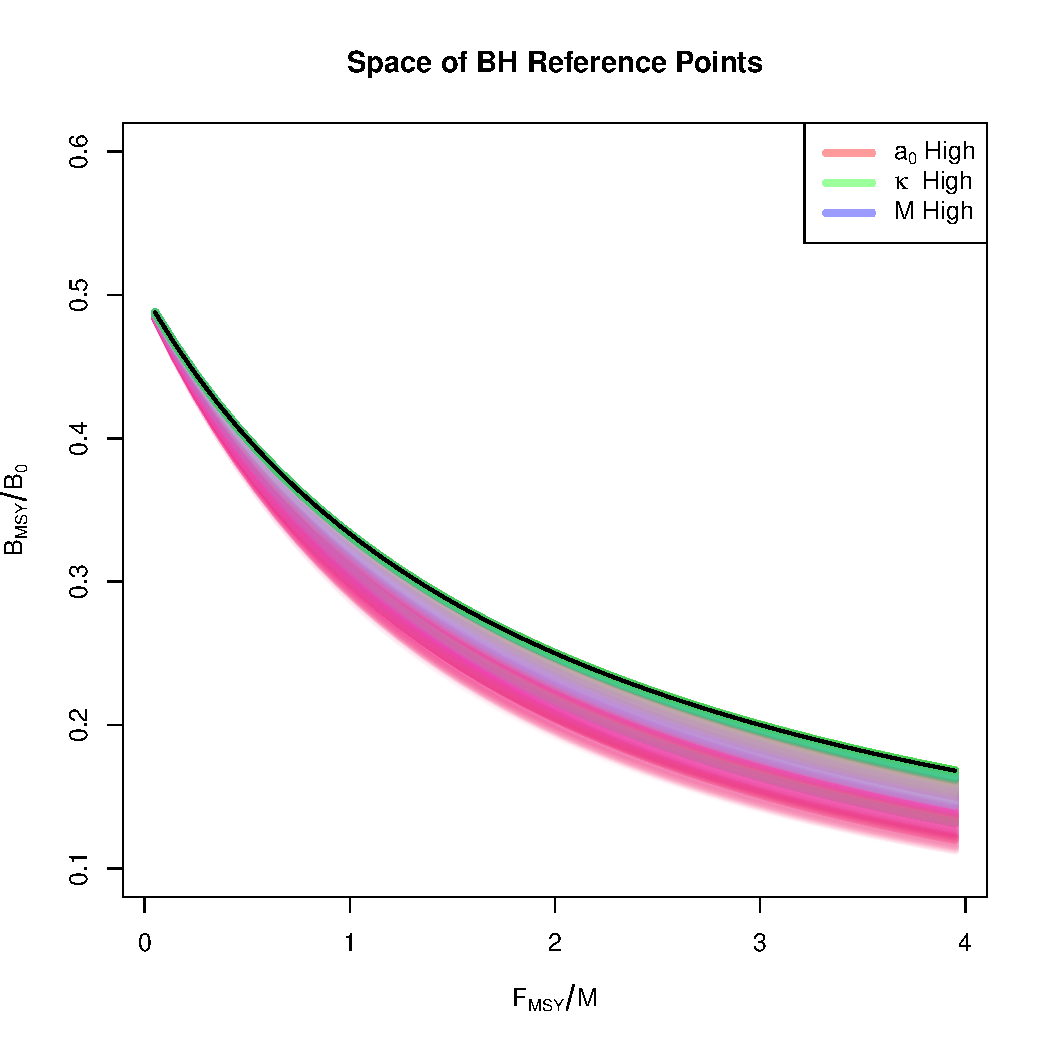
\includegraphics[width=0.5\textwidth]{../ddBias/rpSpace.pdf} 
%
%\vspace{-1cm}
%\caption{
%BH RP-space sensitivity to the parmaters $M$, $\kappa$, and $a_0$. The black 
%curve shows the BH set in the simple production model setting.
%%Yield curves for data generated with $\frac{F^*}{M}=3.48$ and $\frac{B^*}{\bar B(0)}=0.48$.
%%Convert into $B/B_0$. Show the high contrast curve.
%}
%\label{ddRPs}
%\end{figure}
 

%good ideas
\begin{itemize}
\item mapping distance as a function of contrast at (3.5, 0.5)

\item for LHS grid locations show $\frac{B^*}{B_0}$ and $F^*$ biases for grids in $M\in(0,0.5)$ For sure in High Contrast, maybe also in Low??.
\end{itemize}




%%
%\clearpage
%
%%
%\section{Appendix\label{lambApp}: Inverting $\frac{B^*}{\bar B(0)}$ and $\gamma$ for the PT Model}
%For brevity let $\zeta=\frac{B^*}{\bar B(0)}$.
%\begin{align*}
%&\zeta=\left(\frac{1}{\gamma}\right)^{\frac{1}{\gamma-1}}\\
%%&\zeta^{\gamma-1}=\frac{1}{\gamma}\\
%&\zeta=\gamma\zeta^{\gamma}\\
%&\zeta=\gamma e^{\gamma\log(\zeta)}\\
%&\zeta\log(\zeta)=\gamma\log(\zeta) e^{\gamma\log(\zeta)}
%\end{align*}
%The Lambert product logarithm, $W$, is defined as the inverse function of $z=xe^x$ such that $x=W(z)$. 
%Applying this definition allows for the isolation of $\gamma$.
%\begin{align}
%&\gamma\log(\zeta)=W\left(\zeta\log(\zeta)\right) \nonumber\\
%&\gamma=\frac{W\left(\zeta\log(\zeta)\right)}{\log(\zeta)} \label{gammaOfZeta}
%\end{align}
%The Lambert product logarithm is a multivalued function with a branch point at 
%$-\frac{1}{e}$. The principal branch, $W_0(z)$, is defined on $z\in\left(-\frac{1}{e}, \infty\right)$, 
%and the lower branch, $W_{-1}(z)$, is defined on $z\in\left(-\frac{1}{e}, 0\right)$. Taken 
%individually, each respective branch is analytic, but cannot be expressed in terms 
%of elementary functions.
%
%%
%When $\zeta\in\left(0, \frac{1}{e}\right)$ the solution of interest in Eq. (\ref{gammaOfB}) 
%comes from $W_0$. %$\gamma\to1$ as $\zeta\to\frac{1}{e}$ to produce the Fox Model. 
%When $\zeta\to\frac{1}{e}$, the Fox Model emerges as $\gamma\to1$.
%When $\zeta\in\left(\frac{1}{e}, 1\right)$ the solution of interest comes from 
%$W_{-1}$. For the use case presented here, Eq. (\ref{gammaOfB}) is to be interpreted as,
%
%\begin{equation}
%\gamma = 
%\begin{cases} 
%\frac{W_0\left(\zeta\log\left(\zeta\right)\right)}{\log\left(\zeta\right)} & \zeta\in\left(0, \frac{1}{e}\right)\\
%\frac{W_{-1}\left(\zeta\log\left(\zeta\right)\right)}{\log\left(\zeta\right)} & \zeta\in\left(\frac{1}{e}, 1\right)
%\end{cases}. 
%\end{equation} 
%
%%
%Prager 2002, Figure(2).
%
%%goes from $0$ to $1$ the solution of interest starts on the principal branch,
%%and runs toward the 
%%The solution of interest, for the use cases here, come from the 
%%principal branch, often denoted $W_0(z)$. The principal branch of the Lambert 
%%lower branch, often denoted $W_{-1}(z)$.
%%The product logarithm is analytic for $z>-\frac{1}{e}$ , but cannot be expressed 
%%in terms of elementary functions.
%
%
%%principal branch
%https://math.stackexchange.com/questions/3004835/is-the-lambert-w-function-analytic-if-not-everywhere-then-on-what-set-is-it-ana
%https://researchportal.bath.ac.uk/en/publications/algebraic-properties-of-the-lambert-w-function-from-a-result-of-r
%
%%
%https://cs.uwaterloo.ca/research/tr/1993/03/W.pdf
%
%%{\color{blue}
%%%
%%\begin{align}
%%&r = F^*\left( \frac{1-\frac{B^*}{\bar B(0)}}{\frac{B^*}{\bar B(0)}} \right) \left(1-\frac{B^*}{\bar B(0)}\right)^{\left( \frac{\frac{B^*}{\bar B(0)}-1}{\frac{B^*}{\bar B(0)}} \right)}
%%&\gamma = \frac{1}{\frac{B^*}{\bar B(0)}}. \label{rg}
%%\end{align}
%%%{\color{red}
%%%\begin{align}
%%%&r = F^*\left( \frac{\bar B(0)-B^*}{B^*} \right) \left(1-\frac{B^*}{\bar B(0)}\right)^{\left( \frac{B^*-\bar B(0)}{B^*} \right)}
%%%&\gamma = \frac{\bar B(0)}{B^*}.
%%%\end{align}
%%%}
%%
%%}


%%
%%OLD
%%

%BH model 
%%ication of two parameter production functions. 
%%Below 
%RP bias is quantified by the following relative measure of bias, similar to a percent error calculation.
%%
%\begin{align}
%\text{Relative Bias} = \frac{\hat{RP}-RP}{RP}
%\end{align}
%%
%Above $RP$ is a stand-in for the true value of any of the biological
%reference points under the three parameter data generating production model, 
%and $\hat{RP}$ refers to the metamodel estimate of each RP quantity under the 
%%BH model. %two parameter restricted cases.



%{\color{blue}
%\begin{itemize}
%	\item prod parameter to RP transformation
%	\item closing statement about uses
%\end{itemize}
%}


%of RPs %productivity parameters
%with respect to model misspecification of typical two parameter models of 
%productivity (Logistic and BH). 
%
%relative to the model specification 

%%
%%For assessing inference of productivity parameters over the simulated design %, as seen in Figure (\ref{rpGrid}), 
%A GP model is used as a flexible metamodel of how inference responds to various 
%degrees of model misspecification of the restricted model. 
%%
%Design locations, $\bm{X}$, specify the degree of model misspecification relative 
%to the restricted model.
%%
%At each design location of the simulation fitting the restricted two parameter 
%model results in a MLE of each of the productivity parameters 
%(i.e. Schaefer:[$log(r)$, $log(K)$], BH:[$log(\alpha)$, $log(\beta)$]).
%%under the restricted two parameter production model 
%%
%Furthermore, since the maximum likelihood estimator is a random variable, 
%MLE standard error estimates, on the variance scale (via the inverted Fisher 
%information) are also outputs of the simulation.
%%
%Let $\textbf{y}$ be a vector collecting the fitted MLEs for one of the 
%productivity parameters, and let $\bm{\omega}$ be a vector of estimates of the 
%estimator variances at each $\textbf{y}$. 
%%
%This simulation can be seen as the following mapping
%\begin{equation}
%\bm{X} \mapsto \textbf{y} \pm \sqrt{\bm{\omega}}.
%\end{equation}
%%Using the simulation to train a GP metamodel of 
%By constructing a metamodel of this mapping, it allows for a full
%characterization of inference under the misspecified restricted models.
%
%%
%A GP is a stochastic process generalizing the multivariate normal distribution 
%to an infinite dimensional analog. GPs are often specified primarily through the
%choice of a covariance (or correlation) function which defines the relationship 
%between locations in an index set. Typically the index set is spatial for GPs, 
%with points closely related in the index set resulting in correlated effects in 
%the model. In this setting the model is over the space of reference points. 
%A GP model implies an $n$ dimensional multivariate normal distribution on the 
%observations of the model with a correlated error structure defined by the 
%modeled covariance function.










%Letting $\textbf{y}$ be a vector collecting the fitted log productivity parameter MLEs under
%the restricted model, and further letting $\bm{\omega}$ be a vector of the MLE standard error
%estimates, on the variance scale (via the inverted Fisher information of the production model
%log likelihood).
%The simulation produces the following mapping of
%%
%
%
%
%
%a full 
%characterization of inference should To capture the most complete picture of statistical 
%MLE standard error estimates, on the variance scale (via the inverted Fisher information)
%
%
%
%The the farther RP space. 
%
%%As previously established, in Section (\ref{modelFit}), the 
%%biological parameters of interest are the Schaefer model's $log(r)$ and $log(K)$ 
%parameters. Since the estimates of these parameters are random variables, with 
%variances given by the inverse of the observed fisher information, 
%interpolation of MLEs requires paying additional attention to propagating 
%estimates of uncertainty into the metamodel. 

%%Motivate gaussianity
%
%%
%A GP is a stochastic process generalizing the normal distribution to an
%infinite dimensional analog. GPs are often specified primarily through the
%choice of a covariance function which defines the relationship between
%locations in an index set. Typically the index set is spatial for GPs, and in
%this setting the model is across the reference point space, 
%$\left(F^*, \frac{B^*}{\bar B(0)}\right)$, of the three parameter
%PT data generating model. A GP model implies an $n$ dimensional multivariate 
%normal distribution on the observations of the model and the covariance function 
%fills out the covariance matrix for the observations.
%
%%Since covariance between $log(r)$ and $log(K)$ are often indistinguishable 
%%form 0 the interpolator treats
%Modeling the estimates of $log(r)$ and $log(K)$ with independent GP models is 
%used to extend analysis of all major biological RP over the simulated grid. 
%Let $\hat\mu$ be the maximum likelihood estimate (MLE) of either $log(r)$ or 
%$log(K)$. Additionally let $\hat\omega$ be the inverted Hessian information of 
%the log likelihood evaluated at $\hat\mu$. 
%
%%
%Each grid location of the simulation produces a single fitted $\hat\mu_i$ at an
%associate $\left(F^*, \frac{B^*}{\bar B(0)}\right)$ location with 
%$i\in\{1,...,n\}$. $\bm{\hat\mu}$ is jointly modeled over the space of 
%reference points as the following GP,
%%Here the following GP model is used,


%%
%Understanding the effects of productivity model misspecification amounts to 
%understanding 
%
%%
%Each design location of the simulation results in a MLE of each of the productivity
%parameters under the restricted two parameter production model (i.e. Schaefer:[$log(r)$, $log(K)$],
%BH:[$log(\alpha)$, $log(\beta)$]). Since the maximum likelihood estimator is a random 
%variable a full characterization of inference To capture the most complete picture of statistical 
%MLE standard error estimates, on the variance scale (via the inverted Fisher information)
%
%A full characterization of the behavior of statistical 
%inference must also account for estimation uncertainty so each MLE,  
%
%Further, since the simulated process involves statistical inference
%%
%For assessing the productivity parameters over the full region of simulated RPs %, as seen in Figure (\ref{rpGrid}), 
%a GP model is used as a flexible metamodel for describing the overall 
%behavior of inference under the restricted model.



%%
%Letting $\textbf{y}$ be a vector collecting the fitted log productivity parameter MLEs under 
%the restricted model, and further letting $\bm{\omega}$ be a vector of the MLE standard error 
%estimates, on the variance scale (via the inverted Fisher information of the production model 
%log likelihood). 
%The simulation produces the following mapping of 
%%
%\begin{equation}
%\bm{X} \mapsto \textbf{y} \pm \bm{\omega}
%\end{equation}


%%
%Each design location of the simulation produces estimates of two productivity 
%parameters under the restricted two parameter production model (i.e. Schaefer:($r$, $K$), 
%BH:($\alpha$, $\beta$)). 



%%
%For assessing the productivity parameters over the full region of simulated RPs %, as seen in Figure (\ref{rpGrid}), 
%a GP model is used as a flexible metamodel for describing the overall 
%behavior of inference under misspecified two parameter productivity models.
%%
%Each design location of the simulation produces an estimate of each of the productivity   
%parameters under the restricted two parameter production model (i.e. Schaefer:($log(r)$, $log(K)$), 
%BH:($log(\alpha)$, $log(\beta)$)).
%
%%
%\begin{equation}
%\bm{X} \mapsto \textbf{y} \pm \bm{\omega}
%\end{equation}

%\begin{equation*}
%\underbrace{\left(F^*, \frac{B^*}{\bar B(0)}\right)}_{\text{PT Truth}} {\text{GP}\atop{\mapsto\atop~}} \underbrace{\left(\hat F^*, \frac{\hat B^*}{\bar B(0)}\right)}_{\text{Schaefer Estimate}}
%\end{equation*}



%
%As previously established, in Section (\ref{modelFit}), the biological parameters 
%of interest are the Schaefer model's $log(r)$ and $log(K)$ parameters. Since the 
%estimates of these parameters are random variables, with variances given by the 
%inverse of the observed fisher information, interpolation of MLEs requires 
%paying additional attention to propagating estimates of uncertainty into the 
%metamodel.






%
%\clearpage
%{\color{gray}
%\section{Introduction\label{int}}
%
%%
%The most fundamental model in modern fisheries management is the surplus-production 
%model. These models focus on modeling population growth via nonlinear 
%parametric ordinary differential equations (ODE). Key management quantities 
%called reference points (RP) are commonly derived from the ODE equilibrium 
%equations and depend upon the parameterization of biomass production. 
%Two-parameter parameterizations of the production function have been shown to 
%limit the theoretical domain of RPs \shortcite{mangel_perspective_2013}. The 
%limited RP-space of two parameter models are a major source of model 
%misspecification for RPs and thus induce bias in RP estimation. The behavior 
%of RP estimation bias is not well understood and as a result often 
%under appreciated. A metamodeling approach is developed here to describe RP 
%biases and explore mechanisms of model failure in the Schaefer model. 
%%Additionally Sections (\ref{growth} $\&$ \ref{propCatch}) outline additional 
%%projects which will be included in my dissertation. Section (\ref{growth}) 
%%proposes extensions to the immediately following work which generalize results 
%%to a broader set of dynamics. %production functions, as well as proposes an analyze mechanisms of 
%%%model failure in the 
%%%context of simple age structured dynamics. 
%%Section (\ref{propCatch}) proposes a model for incorporating uncertainty in 
%%estimates of catch to better infer biological parameters of the production model.  
%
%%The ODE equilibrium equations Reference points (RP) are key management are derived quantities The equilibrium equation the ODE   
%%
%%%
%%Outline of surplus-production model setting
%%RPs
%%restricted parameter space therefore bias
%%demonstrating and utilizing bias
%%exploring bias 
%
%%NOTE: we can not observe all fish in the sea, and this rely on an index of abundance 
%%which typically comes from experimental fishing procedure(for example ccfrp).
%Data for a typical surplus-production model comes in the form of an index 
%of abundance through time which is assumed to be proportional to the reproducing 
%biomass for the population of interest. The index is often observed alongside 
%a variety of other known quantities, but at a minimum, each observed index 
%will be observed in the presence of some known catch for the period. 
%%The index %of abundance is assumed to be proportional to biomass with the 
%%proportionality %constant being a nuisance parameter that is often referred to 
%%as the %catchability parameter
%%the stock. %a time %%series of observations of an index of abundance for some population of interest. 
%
%%{\color{red}Plot Index Series and Catches}
%\begin{figure}[h!]
%	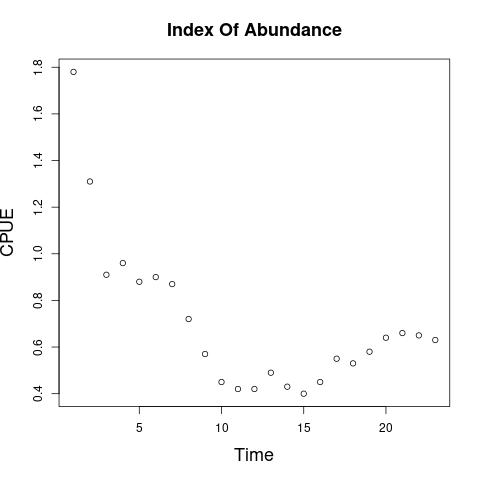
\includegraphics[width=0.5\textwidth]{./plots/hakeIndex.png}
%	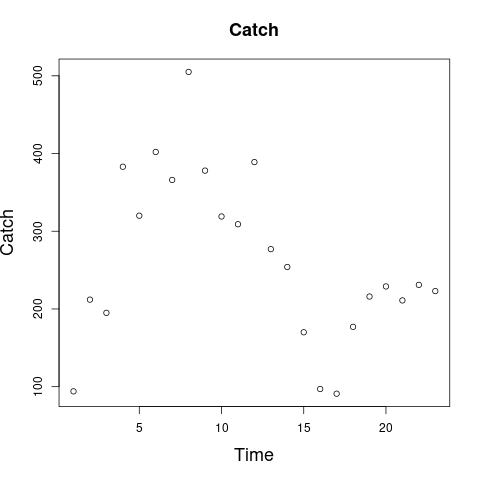
\includegraphics[width=0.5\textwidth]{./plots/hakeCatch.png}
%	\caption{\label{hakeData}
%	\textit{left}: An observed series of index of abundance data for Namibian Hake from 1965 to 1987 \protect\shortcite{hilborn_ecological_1997}.
%	\textit{right}: The associated catch data for Namibian Hake over the same time period.
%	}
%\end{figure}
%
%%
%The observed indices are assumed to have multiplicative log-normal errors, and thus
%the following observation model arises naturally,
%%Pella Tomlinson
%\begin{align}
%I_t = q B_t e^\epsilon ~~~ \epsilon\sim N(0, \sigma^2).
%\end{align}
%%
%Above $q$ is often referred to as the ``catchability parameter''; it serves as the %represents the %$ is often refered to as the catchability parameter and the catchability parameter and 
%proportionality constant mapping between the observed index of abundance and biomass. 
%$\sigma^2$ models residual variation. Biologically speaking $q$ and $\sigma^2$ 
%are often treated as nuisance parameters with the ``biological parameters'' 
%entering the model through a process model on biomass.
%
%% 
%Biomass is assumed to evolve as an ODE; in this case I focus on the following 
%form,
%%
%\begin{equation}
%\frac{dB}{dt} = P(B(t); \bm{\theta}) - C(t). \label{ode}
%\end{equation}
%%$C=FB$ to set up yield calculations later
%Here biomass is assumed to change in time by two processes, net production of 
%biomass into the population, and catches removing biomass from the population.
%
%%  %stock recruitment relationship (SRR). Recruitment 
%Firstly, the population grows through a production function, $P(B)$. Production 
%in this setting is defined as the net biomass increase due to all reproduction 
%and maturation processes accounting for all naturally occurring %no migration the population is assumed closed. 
%sources of mortality other than the recorded fishing from humans. The 
%production function is assumed to be a parametric function that relates the 
%current biomass of the population to an aggregate production of biomass. 
%
%%
%Secondly, the population decreases as biomass is removed due to catch, $C(t)$. 
%While catches (aka yields) are observable quantities \shortcite{pearson_documentation_1997}, %sen_sampling_1984,  
%the model assumes that catch is proportional to biomass with the 
%proportionality constant representing the fishing rate, $F(t)$, so that $C(t)=F(t)B(t)$. 
%From a management perspective a major goal of the model is to accurately infer 
%a quantity known as \emph{maximum sustainable yield} (MSY). One could maximize 
%simple yield at a particular moment in time (and only for that moment) by 
%fishing all available biomass in that moment. This strategy is penny-wise but 
%pound-foolish (not to mention ecologically devastating) since it doesn't leave 
%biomass in the population to reproduce for future time periods. We seek to 
%fish in a way that allows (or even encourages) future productivity in the 
%population. This is accomplished by maximizing the equilibrium level of catch 
%over time. Equilibrium yield is considered by replacing the steady state 
%biomass ($\bar B$) in the assumed form for catch, so that $\bar C = F\bar B(F)$, 
%where $\bar~$ indicates a value at steady state.  Naturally the steady state 
%biomass is a function of $F$; we will see a specific example of this in 
%\mbox{Section (\ref{ptRef}).} MSY is found by optimizing $\bar C(F)$ with respect to 
%$F$, and $F^*$ is the fishing rate at MSY. Going forward let $^*$ decorate any 
%value derived under the condition of MSY.  
%
%% to continue the species and produce  not only are there  however this has the {\color{red}a description of maximum sustainable yield}
%
%%
%%\clearpage
%
%%
%The canonical production model in fisheries is the Schaefer model. The 
%Schaefer model is formed by choosing $P$ to be logistic growth \shortcite{mangel_theoretical_2006} %({\color{red} cite}) 
%parameterized by $\bm{\theta} = [r, K]$ so that the family of production 
%functions takes the following form,  
%%
%\begin{align}
%P(B; [r, K]) = r B \left(1-\frac{B}{K}\right). \label{logistic}
%\end{align}
%$r$ is a parameter controlling the maximum reproductive rate of the population 
%in the absence of competition for resources (i.e. the slope of production 
%function at the origin). $K$ is the so called "carrying capacity" of the 
%population. In this context the carrying capacity can be formally stated as 
%steady state biomass in the absence of fishing \mbox{(i.e. $\bar B(0)=K$).}  
%
%%\begin{wrapfigure}{r}{0.5\textwidth}
%\begin{figure}[h!]
%\begin{minipage}[h!]{0.6\textwidth}
%        \includegraphics[width=\textwidth]{./plots/srrSchaeffer.png}	
%\end{minipage}
%\begin{minipage}[h!]{0.37\textwidth}
%\caption{\label{srrSchaefer}
%	\\The logistic production function in black plotted next to depictions of the key biological parameters and reference points.
%	The slope at the origin (and thus $r$) is shown in blue, catch resulting in MSY in red, biomass at MSY in green, and $K$ in purple at the right x-intercept.	
%	MSY is seen at the peak of the parabola, and is attained with a fishing rate of $\frac{r}{2}$ and biomass equilibrating to $\frac{K}{2}$.
%}
%\end{minipage}
%%\end{wrapfigure}
%\end{figure}
%
%%{
%%\color{red} 
%%Concept of Maximum sustainable yield (MSY)
%%writtting sustainable yield $\bar Y(F) = F\bar B(F)$.
%%}
%
%%%
%%\clearpage
%
%%
%The logistic production function produces idealized parabolic recruitment with 
%equilibrium quantities taking very simple forms that can be easily understood from the 
%graphical construction seen in Figure (\ref{srrSchaefer}). Positive 
%recruitment is observed when \mbox{$B\in(0, K)$.} Due to the parabolic shape of the 
%logistic production function it is straightforward to see that yield is maximized 
%by fishing the stock down to $B^*$, where the stock attains its peak productivity. 
%By symmetry it is clear that this peak occurs at $B^*=\frac{K}{2}$. The fishing 
%rate required to hold the stock at MSY is $F^*=\frac{r}{2}$, which is half of the 
%stocks maximum reproductive rate. \mbox{MSY is then the product of $F^*$ and $B^*$ 
%so that $MSY=\frac{rK}{4}$.}
%%In the absence of fishing $\frac{dB}{dt}$ would be driven entirely by $P$, but at MSY $\frac{dB}{dt}=0$ since the population equilibrates at $B^*$. 
%
%%%
%%{\color{red}
%%While this idealized form is instructive, and convenient, these simplistic 
%%dynamics are also potentially problematic. The symmetry of the logistic 
%%functional form is very rigid in that it assumes dynamics in the lower (mate 
%%limited) regime of the dynamics ($B\in(0, \frac{K}{2})$) have the same shape 
%%as the upper (density limited) regime of the recruitment dynamics 
%%($B\in(\frac{K}{2}, K)$). What in nature ties these phenomena together so that 
%%this assumption should be true? 
%%}
%
%%\clearpage
%%Furthermore, and more practically, 
%%While this idealized form of the logistic production function is instructive, and 
%%convenient, the simplistic dynamics it implies are also potentially problematic.
%Fisheries are very often managed based upon reference points which serve as 
%simplified heuristic measures of population behavior. The mathematical form of 
%RPs depends upon the model assumptions through the production function. %({\color{red} cite}). 
%While a number of different RPs exist which describe the population in different 
%(but related) ways, the most common RPs revolve around the concept of MSY (or robust 
%ways of measuring MSY \shortcite{hilborn_pretty_2010,punt_management_2016}).
%Here the focus is primarily on the RPs $F^*$ and $\frac{B^*}{\bar B(0)}$ for their 
%pervasive use in modern fisheries \shortcite{mangel_perspective_2013,punt_extending_2019}.
%
%%%
%%Here the focus is on two RPs that will be denoted by $\xi$ and $\zeta$ going forward.  
%%% these behaviors that are highly %dependent on the form of the SRR.
%%\begin{align}
%%	&\xi = \frac{F^*}{M}
%%	&\zeta = \frac{B^*}{B_0} \label{xizetaSimple}
%%\end{align}
%
%%
%$F^*$ is the afore mentioned fishing rate which results in MSY. $\frac{B^*}{\bar B(0)}$ 
%is the depletion of the stock at MSY. That is to say $\frac{B^*}{\bar B(0)}$ describes 
%the fraction of the unfished population biomass that will remain in the equilibrium 
%at MSY. In general $F^*\in\mathbb{R}^+$ and \mbox{$\frac{B^*}{\bar B(0)}\in\left(0, 1\right)$,} 
%however under the under the assumption of logistic production these 
%quantities take the following form,  
%%to fish (or rather not to fish) to result in MSY.  
%%based upon$\xi$ is the optimal (in the MSY sense) fishing rate rescaled so that it is in 
%%terms relative to natural mortality. $\zeta$ is the biomass at MSY relative 
%%to the unfished virgin biomass of the population. 
%%
%\begin{align}
%        &F^* = \frac{r}{2}
%        &\frac{B^*}{\bar B(0)} = \frac{1}{2} \label{fbLogistic}
%\end{align}
%so that $\left(F^*, \frac{B^*}{\bar B(0)}\right)\in \left(\mathbb{R}^+, \frac{1}{2}\right)$.
%
%%
%In current practice, production functions are typically chosen to depend only 
%on two parameters. The Schaefer model as presented depends only on
%the biological parameters $r$ and $K$, but other common two parameter choices
%of the production function are the Beverton-Holt \shortcite[BH]{beverton_dynamics_1957} 
%and Ricker \shortcite{ricker_stock_1954} curves. All of these two parameter 
%production functions struggle similarly to model the full theoretical space of 
%RPs \shortcite{mangel_perspective_2013}.
%
%%The Schaefer model is a much loved and argued over model
%The basis of the Schaefer model is ripe with debate \shortcite{kingsland_refractory_1982}, 
%and the debate continues within modern fisheries modeling \shortcite{prager_comparison_2002}. 
%On the one hand, \shortciteA{maunder_is_2003} argues that the Schaefer model is 
%insufficient in large part due to the restriction it places on $\frac{B^*}{\bar B(0)}$, 
%at $\frac{1}{2}$, and further argues that the three parameter Pella-Tomlinson 
%(PT) model \shortcite{pella_generalized_1969} should replace the Schaefer model to avoid biased parameter 
%estimates. On the other hand, while \shortciteA{prager_reply_2003} appreciates 
%the limitations of the Schaefer model, he argues its usefulness as a well 
%understood and simple model that has the ability to reasonably 
%approximate dynamics in many data poor stocks. %productivity shapes. 
%
%%%
%%{\color{red} add to into}
%%bias-variance tradeoff Schaefer high bias, low variance setting. Bias 
%%is the dominant source of estimation error. Variance estimates will be 
%%unrealistically low due to the limited parameter space.
%%
%%%and conversely a two parameter production function will have estimation errrosd. 
%%The argument of \shortciteA{maunder_is_2003} suggests that the two parameter 
%%Schaefer model overly restricts parameter space so that estimation error is unduly 
%%dominated by bias.
%%
%%as to overly limit estimate variances that estimation error is unduly dominated by bias.
%%
%%estimation errors of the two parameter Schaefer model are unduly dominated by bias
%%
%% since the limited parameter 
%%space of the Schaefer model 
%
%%
%The bias-variance trade-off \shortcite{ramasubramanian_machine_2017} makes it 
%clear that the addition of a third parameter in the production function will 
%necessarily reduce estimation bias. However the utility of this bias reduction 
%is still under debate because the particular mechanisms and behavior (direction and magnitude) %over relevant RPs %and mechanisms %behavior 
%of these biases for key management quantities %(and the mechanisms of inducing these biases) 
%are not fully understood or described. \shortciteA{lee_can_2012} provides some 
%evidence that estimation of productivity parameters, and thus RPs via \shortcite{mangel_perspective_2013}, 
%are dependent on biomass contrast as well as model specification. % as well as contrast in data %lacking contrast in biomass. 
%\shortciteA{conn_when_2010} comes to similar conclusions %about steepness estimation
%via calibration modeling techniques. Despite this understanding of productivity estimation, 
%the implications have not been extended to a joint description of biases on the scale of 
%management RPs. % biases jointly.
%
%%The particular behaviors of these RP biases, 
%%and their relationship to each other, are not fully described.  
%
%%Add GOAL of understanding directionality and mechanism of bias.
%%Add claim of novelty by recognizing that bias is a function of RP, a flexible method of propagating estimation uncertainty and accounting for nonlinear bias patterns.
%Together the general behavior of the PT model and the %pragmatic understandable 
%simplicity of the Schaefer model make the PT/Schaefer pair an ideal setting for 
%beginning to understand the consequences of model misspecification on the 
%production function. In this study I consider the behavior of inference when 
%data are simulated from the three parameter PT production model but fit with 
%the two parameter Schaefer model. 
%
%%
%The work begins with a derivation of RPs under the three parameter PT model. 
%The parametric forms of RPs under the PT model are then inverted to develop a 
%simulation setting for analyzing inference under the two parameter Schaefer 
%model. Finally a Gaussian Process (GP) metamodel \shortcite{gramacy_surrogates_2020} is constructed for exploration 
%and analysis of RP biases. 
%
%%
%A key insight of this approach is that bias is considered broadly across RP-space to 
%uncover patterns and correlations between RPs. %f bias magnitude and direction. 
%%A flexible Gaussian Process (GP) meta-modeling approach is used to model bias 
%%patterns across RP-space. 
%The GP metamodel is explicit about trade-offs between RPs %to the surface bias tradeoffs to the surface to 
%so as to inform the full utility of reducing bias, as well as to suggest mechanisms for 
%understanding what causes bias. Further, the effect of contrast on estimation 
%is considered together with model misspecification. %alongside the effect of model misspecification.  
%
%}
%
%
%%Inverting the RP parametric forms is used to develop a simulation setting for 
%%controlling the degree and nature of model misspecification 
%
%%%
%%{\color{gray}
%%\begin{itemize}
%%\item[\checkmark] Lead into this reaserch with other studies (Lit review)
%%\item Emphasize a clear statement of the study goal
%%\item a statement of novelty
%%	\begin{itemize}
%%	\item[\checkmark] model misspecification leads to bias
%%	\item[Sorta] non-constant bias of RP-space (a holistic summary of model performance.)
%%	\item[Sorta] methodology to account for bias in the presence of uncertainty
%%	\end{itemize}
%%\end{itemize}
%%}
%
%%using the two parameter Schaefer model to fit data that are generated from 
%
%
%
%%Since the Schaefer model is more restrictive than the PT model, estimates of RPs 
%%arrived at from the Schaefer model must necessarily be biased relative to the 
%%true PT RPs. Given the ubiquity of two parameter productions functions in 
%%management it is of paramount importance to understand the biasing lens 
%%through which we've come to understand our fisheries.
%
%
%
%%only a slightly more complex production function which can full accommodate RP space. 
%%Namely data are simulated from the %can full  the full space of RPs. I consider data 
%%simulated from the 
%%three parameter Pella-Tomlinson (PT) production model. 
%
%
%
%%%
%%In practice, at this time, the production function is typically chosen to depend 
%%only on two parameters. The Schaefer model as presented depends only on 
%%the biological parameters $r$ and $K$, but other common two parameter choices 
%%of the production function are the Beverton-Holt (BH) and Ricker curves. All
%%of these two parameter production functions struggle similarly to model the full 
%%theoretical space of RPs \shortcite{mangel_perspective_2013}.
%
%
%
%%{\color{gray}
%%%
%%Schaefer model clearly insufficient but can be made to estimate some parameters correctly Prager 2002, Prager 2003.
%%Francis 2012/Lee 2011
%%        assessment model correctly specified
%%Lee 2012
%%        contrast estimate steepness
%%Instructive in its simplicity Prager 2003.
%%
%%%
%%PT generalizes Schaefer Maunder 2003
%%Three parameter PT should supplant Schaefer
%%
%%%
%%Other functions recommended in practice BH Punt 2005 or Ricker. 
%%Although statistically differentiating the models is difficult Dorn 2002, Brodziak 2002 
%%BH and Ricker suffer from the similar model deficiencies Mangle 2013 as the Schaefer does for the PT relating the reduced decrees of freedom in the parameter space.
%%
%%%
%%Punt 2019 move toward 3 parameter models
%%
%%%
%%Punt 2019 move toward 3 parameter models
%%Punt 2005 recommends BH and expansion into 3 parameters
%%Maunder 2003
%%	PT generalizes and should supplant Schaefer
%%	"shape" parameter B*/B0
%%	Bias variance trade off between PT3 Vup/Bdown and Logistic Vdown/Bup
%%Francis 2012/Lee 2011
%%	assessment model correctly specified
%%Lee 2011
%%	contrast estimate steepness
%%Field 2009 Bacaccio BH v. Stanley 2009 Ricker 
%%zeta=0.39		  zeta=0.5
%%
%%%
%%\begin{itemize}
%%\item[\checkmark] Lead into this reaserch with other studies (Lit review)
%%\item Emphasize a clear statement of the study goal
%%\item a statement of novelty
%%	\begin{itemize}
%%	\item[\checkmark] model misspecification leads to bias
%%	\item[Sorta] non-constant bias of RP-space (a wholistic summary of model performance.)
%%	\item[Sorta] methodology to account for bias in the presence of uncertainty
%%	\end{itemize}
%%\end{itemize}
%%}
%
%
%
%
%%and subsequently fit these 
%%data using the two parameter Schaefer model to observe the consequences of 
%%SRR model-misspecification with special interest on RP management quantities.  
%
%%%than the most commonly used in practice but
%%{\color{gray}
%%%All models are wrong but some are useful {\color{red}(cite or remove)}. 
%%{\color{red}
%%Nature does not generate data from a simple model. However, what would happen if 
%%nature were even just slightly more complex than the most commonly used fisheries 
%%models? I consider data simulated from the three parameter Pella-Tomlinson (PT) 
%%SRR model, and subsequently fit these data using the two parameter Schaefer 
%%model to observe the consequences of SRR model-misspecification with special 
%%interest on RP management quantities.  
%%}
%
%%What would happen if 
%%data were to truly be generated from a three parameter SRR model and further 
%%what would be the consequence of misspecifying a two parameter model only as a 
%%special case of the true three parameter model? 
%%
%%%
%%Data are simulated from the three parameter Pella-Tomlinson SRR model, and 
%%subsequently fit using the two parameter Schaefer model. RP 
%%%
%%{\color{red} Outline simulation goal, end introduction, and start methods.}
%
%%\begin{itemize}
%%\item[\checkmark] introduce fisheries type data
%%\item[\checkmark] ODE modeling formulation
%%\item[\checkmark] Schaefer Model (Logistic production function)
%%\item[\checkmark] Reference Points
%%{\color{gray}\item Pella-Tomlinson production function}
%%\item[\checkmark] general simulation idea
%%\end{itemize}
%
%
%%
%%\clearpage
%\section{Methods}
%
%
%%Construct RP under PT production
%
%%
%\subsection{PT Model}
%
%{\color{gray}
%%Below I present the three parameter Pella-Tomlinson (PT) family, which has a 
%The three parameter PT family has a convenient form that includes, among 
%others \shortcite{fox_jr_exponential_1970,rankin_alternative_2015}, the 
%logistic production function as a special case to form the Schaefer model. The 
%Pella-Tomlinson production function is parameterized so that $\bm{\theta} = [r, K, \gamma]$ 
%and the family takes the following form, 
%%Pella Tomlinson
%\begin{align}
%P(B; [r, K, \gamma]) = \frac{r B}{\gamma-1} \left(1-\frac{B}{K}\right)^{\gamma-1}. \label{pellaTomlinson}
%\end{align}
%%
%
%%
%$\gamma$ is a parameter which breaks PT out of the restrictive symmetry of the 
%logistic curve. In the special case of $\gamma=2~~$ Eq (\ref{pellaTomlinson}) 
%collapses back to the logistic curve, however in general $\gamma\in(1, \infty)$.
%The parameters $r$ and $K$ maintain the same interpretation as 
%they do in the logistic production function. In Figure (\ref{srrPT}) PT recruitment 
%is shown for a range of parameter values so as to demonstrate the various 
%recruitment shapes that can be achieved by PT recruitment.  
%%{\color{red} And $\gamma$ is a parameter which adds 
%%flexibility to the family by allowing for compensatory or non-compensatory 
%%growth. (break symmetry... get better description) }
%
%%\begin{wrapfigure}{r}{0.5\textwidth}
%\begin{figure}[h!]
%	\centering
%	\includegraphics[width=0.49\textwidth]{./plots/srr1.1.png}	
%	\includegraphics[width=0.49\textwidth]{./plots/srr2.png}
%	\caption{\label{srrPT}
%	(\emph{left}) PT production functions with parameters chosen so that MSY is consistent, but $\frac{B^*}{\bar B(0)}$ is less than $\frac{1}{2}$ (in red), greater than $\frac{1}{2}$ (in blue), or equal to $\frac{1}{2}$ (in black; logistic production function).
%	(\emph{right}) PT production functions over a range of $\gamma$ values with the values of $r$ and $K$ fixed at 1 and 10,000 respectively.  
%	}
%\end{figure}
%%\end{wrapfigure}
%
%%\begin{figure}[h!]
%%\begin{minipage}[h!]{0.349\textwidth}
%%\hspace*{-1cm}
%%\includegraphics[width=1.05\textwidth]{./plots/srr1.1.png}
%%\end{minipage}
%%\begin{minipage}[h!]{0.349\textwidth}
%%\hspace*{-1cm}
%%\includegraphics[width=1.05\textwidth]{./plots/srr2.png}
%%\end{minipage}
%%\begin{minipage}[h!]{0.29\textwidth}
%%\hspace*{-0.5cm}
%%\vspace*{-0.75cm}
%%\caption{\label{srrPT}\\
%%	(\emph{left}) PT production functions with parameters chosen so that MSY is consistent, but $\frac{B^*}{\bar B(0)}$ is less than $\frac{1}{2}$, greater than $\frac{1}{2}$, or equal to $\frac{1}{2}$.
%%	(\emph{right}) PT production functions over a range of $\gamma$ values with the values of $r$ and $K$ fixed at 1 and 10,000 respectively.  
%%}
%%\end{minipage}
%%\end{figure}
%
%
%%
%\clearpage
%
%%
%While the particular form of how $\gamma$ appears in PT still produces some 
%limitations to the form of the production function, importantly the 
%introduction of a third parameter allows enough flexibility to fully describe 
%the space of reference points used in management. To see this, the reference 
%points are analytically derived for the PT model below. % in the following section.
%
%%%
%%\begin{equation}
%%\frac{dB}{dt} = P - FB.
%%\end{equation}
%
%%}
%
%%
%\subsection{PT Reference Points}\label{ptRef}
%
%%
%With $B(t)$ representing biomass at time $t$, under PT production, the 
%dynamics of biomass are defined by the following ODE,
% 
%\begin{equation}
%\frac{dB}{dt} = \frac{r B}{\gamma-1} \left(1-\frac{B}{K}\right)^{\gamma-1} - FB. \label{odePT}
%\end{equation}
%
%An expression for the equilibrium biomass is attained by setting Eq (\ref{odePT}) 
%equal to zero, and rearranging the resulting equation to solve for $B$. 
%Thinking of the result as a function of $F$ gives, 
%%When thought of as a 
%%function of $F$ the following expression emerges,
%%{\color{red}Under Pella-Tomlinson SRR the equilibrium biomass can be written,}
%\begin{align}
%\bar B(F) = K\left(1-\left(\frac{F(\gamma-1)}{r}\right)^{\frac{1}{(\gamma-1)}}\right). \label{Beq}
%\end{align}
%
%%By definition $B_0=K$. Alternatively, Setting $F=0$ in Eq(\ref{Beq}) makes it convenient to notice that $\bar B(0)=K$ to arrive at the same result
%At this point it is convenient to notice that $\bar B(0)=K$. The expression for $B^*$ is given by evaluating Eq (\ref{Beq}) at $F^*$.
%
%%
%To get an expression for $F^*$, the equilibrium yield is maximized with respect to $F$,
%\begin{equation}
%F^* = \argmax_F F\bar B(F).
%\end{equation}
%%
%In the case of PT production this maximization can be done analytically (however 
%many three parameter production functions do not result in tractable analytical 
%solutions). In this case maximization can proceed by differentiating the 
%equilibrium yield with respect to $F$ as follows,
%
%%
%\begin{align}
%\frac{d \bar{Y}}{dF} &= \bar B(F) + F \frac{d \bar B}{dF} \label{Fderiv}\\
%%\frac{d \bar B}{dF} &= -\frac{K}{\gamma-1}\left(\frac{\gamma-1}{r}\right)^{\frac{1}{\gamma-1}}F^{\frac{1}{\gamma-1}-1}\\
%\frac{d \bar B}{dF} &= -\frac{K}{F(\gamma-1)}\left(\frac{F(\gamma-1)}{r}\right)^{\frac{1}{\gamma-1}}\label{dBdF}.
%\end{align}
%%{\color{red}
%Setting Eq (\ref{Fderiv}) equal to 0, substituting $\bar B(F)$ and 
%$\frac{d \bar B}{dF}$ by Equations (\ref{Beq}) and (\ref{dBdF}) respectively, 
%and then solving for $F$ produces the following expression for the fishing 
%rate required to produce MSY, %{\color{red}Below any quantity evaluated at MSY shall be decorated with $~^*$.}
%%
%\begin{align}
%F^* = \frac{r}{\gamma-1} \left(\frac{\gamma-1}{\gamma}\right)^{\gamma-1}. \label{Fmsy}
%\end{align}
%%
%Plugging the above expression for $F^*$ back into Eq (\ref{Beq}) gives the 
%following expression for biomass at MSY, 
%\begin{align}
%B^* = \frac{K}{\gamma} \label{Bmsy}. %\left(1-\left(\frac{\gamma-1}{\gamma}\right)\right) \label{Bmsy}.
%\end{align}
%
%%
%The above derived expressions for $\bar B(0)$, $B^*$, and $F^*$ can then be used to 
%build a specific analytical form for the biological reference points in terms of only 
%biological model parameters.
%%%
%%By substituting the expressions given above for $B_0$, $B^*$, and $F^*$ into 
%%Eq(\ref{xizetaSimple}), $\xi$ and $\zeta$ can take a specific analytical form 
%%in terms of the biological model parameters. 
%%%given by substituting the expressions given in Eq(\ref{Fmsy}) 
%%%and Eq(\ref{Bmsy}) in Eq(\ref{xizetaSimple}).
%%%Eq(\ref{xizetaSimple}) can then take a specific analytical form in terms of the 
%%  %an expression for $\xi$ and $\zeta$ can be found in terms of model parameters.  
%\begin{align}
%&F^* = \frac{r}{(\gamma-1)} \left(\frac{\gamma-1}{\gamma}\right)^{\gamma-1}
%&\frac{B^*}{\bar B(0)} = \frac{1}{\gamma} %1-\left(\frac{\gamma-1}{\gamma}\right)
%\end{align}
%
%%{\color{red}demonstration of the restricted case with graph over RP space as used.}
%
%\subsection{Simulation Study \label{sim}}
%
%%
%Indices of abundance are simulated from the three parameter PT production model 
%over a grid of $F^*$ and $\frac{B^*}{\bar B(0)}$ values. These PT data are then 
%fit with a two parameter Schaefer model. 
%%$\gamma$ is then fixed to two so that the PT SRR reduces to the special case of logistic recruitment. 
%%The restricted Schaefer model is then fit to the 
%%simulated PT indices. 
%
%%%
%%
%%Let $\tilde~$ decorate any quantity that is derived under the restricted two 
%%parameter SRR.\\ Collapse to the case of Schaefer. Similarly to Eq(\ref{
%%logisticSRR}) setting $\gamma=2$ results in the equilibrium equations for the 
%%restricted Schaefer model.  
%% 
%
%%speaking it is not possible to analytically invert this  
%Generating simulated indices of abundance from the PT model requires 
%inverting the relationship between $\left(F^*, \frac{B^*}{\bar B(0)}\right)$, and 
%$(r, \gamma)$. It is not generally possible to analytically invert this 
%relationship for many three parameter production functions \shortcite{punt_extending_2019, schnute_analytical_1998}. %{(\color{red}cite Derizo paper)}. 
%Most three parameter production functions lead to RPs that require expensive 
%numerical methods to invert; more over the numerical inversion procedure can %is 
%often be unstable. That said, for the case of PT this relationship is 
%analytically invertible, and leads to the following relationship
%
%%
%\begin{align}
%&r = F^*\left( \frac{1-\frac{B^*}{\bar B(0)}}{\frac{B^*}{\bar B(0)}} \right) \left(1-\frac{B^*}{\bar B(0)}\right)^{\left( \frac{\frac{B^*}{\bar B(0)}-1}{\frac{B^*}{\bar B(0)}} \right)}
%&\gamma = \frac{1}{\frac{B^*}{\bar B(0)}}. \label{rg}
%\end{align}
%%{\color{red}
%%\begin{align}
%%&r = F^*\left( \frac{\bar B(0)-B^*}{B^*} \right) \left(1-\frac{B^*}{\bar B(0)}\right)^{\left( \frac{B^*-\bar B(0)}{B^*} \right)}
%%&\gamma = \frac{\bar B(0)}{B^*}.
%%\end{align}
%%}
%
%%
%%\clearpage
%
%%
%Indices are generated under the following conditions. Data are simulated at
%each point on the grid $\mathcal{F}\times\mathcal{B}$, with $F^*\in\mathcal{F}$ 
%and $\frac{B^*}{\bar B(0)}\in\mathcal{B}$, where $\mathcal{F}=\{0.1, 0.2, ..., 0.7\}$ 
%and $\mathcal{B}=\{0.2, 0.3, ..., 0.6\}$ as seen in Figure (\ref{rpGrid}).  
%These ranges of values for $F^*$ and $\frac{B^*}{\bar B(0)}$ are selected to 
%include a wide range of values thought to reflect many commonly assessed fisheries.
%%commonly  of most commonly assessed fish species {\color{red}cite}. 
%The red X's in Figure (\ref{rpGrid}) show four simulation locations where the 
%Schaefer model is misspecified to a large degree and will be considered in more 
%detail in \mbox{Section(\ref{flat}).} For each $\left(F^*, \frac{B^*}{\bar B(0)}\right)$, 
%the associated pair $(r, \gamma)$ are computed from \mbox{Eq (\ref{rg}).} Since $K$ 
%does not enter the RP calculation its value is fixed arbitrarily at 10000.  %A relatively large value of $K$ is selected to allow a full range of population dynamics to be defined in this setting. The value of $M$ is fixed at 0.2 to represent {\color{red}species}. 
%The value of $q$ is fixed at a typically small value of 0.0005. $\sigma$ is 
%fixed at the relatively small value of 0.01 to focus specifically on the 
%behavior of population parameters. These parameters fully specify the PT 
%model for the purposes of generating index data for each $\left(F^*, \frac{B^*}{\bar B(0)}\right)$ pair.
%
%
%%
%$~$\\
%\begin{figure}[h!]
%\hspace*{0.5cm}
%\begin{minipage}[h!]{0.6\textwidth}
%\includegraphics[width=\textwidth]{../present/shaeferDat.png}
%\end{minipage}
%\begin{minipage}[h!]{0.3\textwidth}
%\caption{\label{rpGrid}\\
%Open circles show the \mbox{location} of the simulation grid \mbox{$\mathcal{F}\times\mathcal{B}$.}
%The \mbox{horizontal} line shows the \mbox{constrained} space of RPs for the \mbox{Schaefer} model.
%The red X's indicated 4 simulation locations where the \mbox{Schaefer} model is particularly 
%misspecified.
%}
%\end{minipage}
%\end{figure}
%%%
%%\begin{figure}[h!]
%%\begin{minipage}[h!]{0.53\textwidth}
%%\includegraphics[height=0.37\textheight]{../present/shaeferDat.png}
%%\end{minipage}
%%\begin{minipage}[h!]{0.48\textwidth}
%%\caption{\label{rpGrid}
%%Open circles show the location of the simulation grid $\mathcal{F}\times\mathcal{B}$.
%%The horizontal line shows the constrained space of RPs for the Schaefer model.
%%The red X's indicated 4 simulation locations where the Schaefer model is particularly 
%%misspecified.
%%}
%%\end{minipage}
%%\end{figure}
%
%%
%\clearpage
%\subsection{Catch \label{catch}}
%
%%%
%%For the sake of simulation, catch is parameterized so that $F_t$ can be 
%%controlled with respect to $F^*$. 
%
%%
%It is known that the behavior of catch can effect inference on the biological 
%parameters \shortcite{hilborn_quantitative_1992}. % {\color{red} cite walters}). 
%In particular it is thought that catch can induce "contrast" in index data
%so as to better inform $r$. In this setting contrast refers to changes in the 
%long term trends of index data. Figure (\ref{expCatchT45}, \emph{right}) demonstrates an 
%example of biomass that includes contrast induced by catch. It is not well 
%understood how contrast may factor into biases induced by model misspecification. 
%To investigate this a variety of catches are investigated.
%%the role that 
%%catch plays in understanding model misspecification errors a variety of 
%%catches are investigated.  
%
%%
%Catch is parameterized so that $F(t)$ can be controlled with respect to $F^*$. 
%Recall that catch is assumed to be proportional to biomass with the 
%proportionality constant amounting to the fishing rate, so that $C(t)=F(t)B(t)$. 
%To control $F(t)$ with respect to $F^*$, $C(t)$ is specified by defining the 
%quantity $\frac{F(t)}{F^*}$ as the relative fishing rate. $B(t)$ is defined 
%by the solution of the ODE, and $F^*$ is defined by the biological parameters 
%of the model, see Eq (\ref{Fmsy}).  Thus by defining 
%$\frac{F(t)}{F^*}$, catch can then be written as \mbox{$C(t)=F^*\left(\frac{F(t)}{F^*}\right)B(t)$.}
%
%%
%Intuitively $\frac{F(t)}{F^*}$ describes the fraction of $F^*$ that $F(t)$ is  
%specified to for the current $B(t)$. When $\frac{F(t)}{F^*}=1$, $F(t)$ will be 
%held at $F^*$, and the solution of the ODE brings $B(t)$ into equilibrium at 
%$B^*$. For constant $\frac{F(t)}{F^*}$ the Schaefer model 
%%has an analytical 
%%solution, via integrating factors, so that $B(t)$ 
%comes to equilibrium as an exponential decay from $K$ approaching $B^*$. The relative fishing rate is defined on $[0, \infty)$; when 
%$\frac{F(t)}{F^*}<1$, $F(t)$ is lower than $F^*$ and $B(t)$ is pushed toward 
%$\bar B>B^*$. Contrarily, when $\frac{F(t)}{F^*}>1$, $F(t)$ is higher than 
%$F^*$ and $B(t)$ is pushed toward $\bar B<B^*$; the precise values of $\bar B$
%can be calculated from Eq (\ref{Beq}).
%
%%
%In practice, catch is determined by a series of observed, assumed known, catches. 
%Catch observations are typically observed on a quarterly (or yearly) basis, so 
%that the ODE may be discretized via Euler’s method with integration step sizes 
%to match the observation frequency of the modeled data. In this case, catch is sampled 
%as would be done in practice however, the simulation can encounter a variate of issues 
%working with the naively discretized ODE. As a result the ODE is integrated implicitly 
%via the Livermore Solver \shortcite[lsode]{radhakrishnan_description_1993}, and catch 
%is linearly interpolated between sampled epochs. 
%%More detail about issues of continuity and ODE integration are described in 
%%Appendix (\ref{appODE}).
%
%%\begin{itemize}
%%	%\item how its parameterized
%%	%\item different behaviors
%%	%\item contrast
%%	\item Forcing function
%%	\item continuity and the solution of ODEs
%%\end{itemize}
%
%%
%\clearpage
%\subsection{Model Fitting\label{modelFit}}
%
%%
%The goal of model fitting is to assess how the biological parameters of the 
%two parameter Schaefer model behave under MLE inference when fit to PT data. 
%Thus, let $I_t$ be an observation of PT index data at time $t\in\{1,2, 3,..., T\}$. The observation 
%model is log-normal such that,
%%
%\begin{align}
%I_t| q, \sigma^2, \bm{\theta} \sim LN(qB_t(\bm{\theta}), \sigma^2).
%\end{align}
%
%For the Schaefer model $\bm{\theta}=[r, K]$, and $B_t(\bm{\theta})$ is defined 
%by the solution of the following ODE
%%
%\begin{align}
%\frac{dB}{dt} = r B \left(1-\frac{B}{K}\right) - FB. \label{odeS}
%\end{align}
%
%The $I_t$ are assumed independent conditional on $q$, $\sigma^2$, $r$, $K$ 
%and the ODE model for biomass. Thus the log likelihood can be written as 
%%
%\begin{align}
%\log\mathcal{L}(q, \sigma^2, \bm{\theta}; I) = - \frac{T}{2}\log(\sigma^2) - \frac{1}{2\sigma^2}\sum_t \log\left(\frac{I_t}{qB_t(\bm{\theta})}\right)^2. \label{logLike}
%\end{align}
%
%%
%In this setting, $q$ is fixed at the true value of 0.0005 to focus on the 
%inferential effects of model misspecification on biological parameters. 
%$\sigma^2$, $r$, and $K$ are reparameterized into the log scale as 
%$log(\sigma^2)$, $log(r)$, and $log(K)$ and fit via MLE. $\sigma^2$ is
%allowed to be fit to assess overall model fit. Reparameterization 
%of the parameters into the log scale improves the reliability of optimization
%in addition to facilitating the use of Hessian information for parameter 
%estimate standard errors.
%%$r$ and $K$ are reparameterized as $log(r)$ and $log(K)$ to improve the regularity of 
%
%%
%Given that the biological parameters enter the likelihood via a nonlinear ODE, 
%and further the parameters themselves are related to each other nonlinearly, 
%the likelihood function can often be difficult to optimize. A hybrid optimization 
%scheme is used to maximize the log likelihood to ensure that a global MLE solution 
%is found. The R package GA \shortcite{scrucca_ga_2013, scrucca_extensions_2017} is 
%used to run a genetic algorithm to explore parameter space globally. 
%Optimization occasionally jumps into the L-BFGS-B local optimizer to refine 
%optima within a local mode. The scheme functions by searching globally to 
%iteratively improve hot starts for the local optimizer. 
%
%%\ref{appMLE}
%In Appendix A a profile likelihood method for estimating all of the 
%parameters of the model is derived. The profile likelihood technique greatly 
%improves the reliability of local optimizers when fitting the biological parameters 
%alongside additional nuisance parameters. The catchability parameter $q$ has the 
%effect of rescaling biomass which can often function similarly to the role of the 
%carrying capacity parameter $K$. Thus, the structure of the likelihood may 
%confound $q$ and $K$, and for some data these parameters may only be weakly 
%identifiable. Posing the model in a Bayesian context provides a convenient 
%mechanism for managing these weak identifiability issues. In a tactful Bayesian 
%formulation $q$ and $\sigma^2$ may then be marginalized out of the joint posterior 
%to yield fast and reliable inference \shortcite{walters_calculation_1994}. %deyoreo_integrating_2012}. %deyoreo_integrating_nodate}. %({\color{red} Cite Maria DeYorio pdf}).
%
%
%% $q$ procedure
%%  
%%%
%%By working with the resulting models parameterized in terms of 
%%$\log(\tilde F^*)$ it tends to improve optimization convergence. Furthermore, 
%%the normality this induces on the log scale, via the Laplace approximation, 
%%yields Log-Normality on $\tilde F^*$, as seen in Appendix {\ref{appA}}. 
%
%%
%\subsection{Gaussian Process Metamodel}
%%
%
%%
%For assessing biological parameters over the simulated grid, as seen in 
%Figure (\ref{rpGrid}), a GP model is used as a flexible, stochastic interpolator 
%over RP space. As previously established, in Section (\ref{modelFit}), the 
%biological parameters of interest are the Schaefer model's $log(r)$ and $log(K)$ 
%parameters. Since the estimates of these parameters are random variables, with 
%variances given by the inverse of the observed fisher information, 
%interpolation of MLEs requires paying additional attention to propagating 
%estimates of uncertainty into the metamodel. 
%
%%Motivate gaussianity
%
%%
%A GP is a stochastic process generalizing the normal distribution to an
%infinite dimensional analog. GPs are often specified primarily through the
%choice of a covariance function which defines the relationship between
%locations in an index set. Typically the index set is spatial for GPs, and in
%this setting the model is across the reference point space, 
%$\left(F^*, \frac{B^*}{\bar B(0)}\right)$, of the three parameter
%PT data generating model. A GP model implies an $n$ dimensional multivariate 
%normal distribution on the observations of the model and the covariance function 
%fills out the covariance matrix for the observations.
%
%%Since covariance between $log(r)$ and $log(K)$ are often indistinguishable 
%%form 0 the interpolator treats
%Modeling the estimates of $log(r)$ and $log(K)$ with independent GP models is 
%used to extend analysis of all major biological RP over the simulated grid. 
%Let $\hat\mu$ be the maximum likelihood estimate (MLE) of either $log(r)$ or 
%$log(K)$. Additionally let $\hat\omega$ be the inverted Hessian information of 
%the log likelihood evaluated at $\hat\mu$. 
%
%%
%Each grid location of the simulation produces a single fitted $\hat\mu_i$ at an
%associate $\left(F^*, \frac{B^*}{\bar B(0)}\right)$ location with 
%$i\in\{1,...,n\}$. $\bm{\hat\mu}$ is jointly modeled over the space of 
%reference points as the following GP,
%%Here the following GP model is used,
%\begin{align}   \label{gpModel}
%        \bm{x} &= \left(F^*, \frac{B^*}{\bar B(0)}\right) \nonumber\\
%        \hat\mu &= \beta_0 + \bm{\beta}'\bm{x} + f(\bm{x}) + \bm{\epsilon} \nonumber \\
%        f(\bm{x}) &\sim \text{GP}(0, \tau^2 R(\bm{x}, \bm{x'})) \nonumber \\
%        \epsilon_i &\sim \text{N}(0, \hat\omega_i).
%\end{align}
%%
%The GP residual variation provides an ideal mechanism for propagating uncertainty 
%from inference in the simulation step into the metamodel. $\hat\omega_i$ is the 
%observed residual variation for the inferred value, $\hat\mu_i$. This mechanism 
%down weights the influence of each $\hat\mu_i$ in proportion to the inferred 
%sampling distribution uncertainty. This has the effect of smoothing the GP 
%model in a way similar to the nugget effect \shortcite{gramacy_cases_2012}. %({\color{red} cite nugget paper})
%% from inference in the simulation step. 
%%This allows for the full propagation of inferred information 
%%from the simulation step to be propagated into the reference point meta-model.
%
%%The GP residual 
%%variation provides an ideal mechanism for propagating this uncertainty while 
%%allowing for a wide class of flexible interpolating functions.
%
%%
%Here $R$ is the squared exponential correlation function.
%\begin{align}   \label{corModel}
%R(\bm{x}, \bm{x'}) &= \exp\left( \sum_{j=1}^2 \frac{-(x_j-x'_j)^2}{2\ell_j^2} \right) %\bm{\Lambda}^{-1} (\bm{x}-\bm{x'}) \right) \nonumber\\ %\norm{\bm{x}-\bm{x'}}_{\bm{\Lambda}}; \nu) \nonumber\\
%%%\norm{\bm{x}-\bm{x'}}_{\bm{\Lambda}} &= \sqrt{ (\bm{x}-\bm{x'})^\top \bm{\Lambda}^{-1} (\bm{x}-\bm{x'}) } \nonumber\\
%%\bm{\Lambda} &=
%%        \begin{pmatrix}
%%                \lambda_\xi & 0\\
%%                0 & \lambda_\zeta
%%        \end{pmatrix}.
%\end{align}
%$R$ has an anisotropic separable form to allow for differing length scales in 
%the $F^*$ and $\frac{B^*}{\bar B(0)}$ axes. The flexibility to model 
%correlations separately in the different RP axes is key due to the 
%differences in the extent of the RP domains marginally. $\ell_1$ and 
%$\ell_2$ model the length scales for $F^*$ and $\frac{B^*}{\bar B(0)}$ 
%respectively. The metamodel parameters $\beta_0$, $\bm{\beta}$, $\tau^2$, 
%$\ell_1$ and $\ell_2$ are fit via MLE against the observations of $\hat\mu$ 
%and $\hat\omega$ from  simulation fits. 
%
%%
%Predictive estimates of modeled quantities are obtained via kriging over 
%intermediate values over RP space. Let $\check~$ decorate any quantity that is 
%derived for metamodel interpolation.
%%{\color{red}Let $\tilde~$ decorate any quantity that is derived 
%%under the metamodel prediction.}
%
%\begin{equation}
%	\check \mu(\check s) = \beta_0 + \bm{x}(\check s)\bm{\beta} + {R}_{\bm{\ell}}(\check s, s) {R}^{-1}_{\bm{\ell}}(s, s)\Big({\hat\mu}(s)-\big(\beta_0+\bm{x}(s)\bm{\beta}\big)\Big)
%\end{equation}
%
%%
%}
%
%%%
%%{\color{orange}
%%\begin{itemize}
%%\item GP serves as a flexible, stochastic interpolator for understanding the basic behavior of 
%%biases induced my limiting the SRR model.  
%%\item This model allows for the full propagation of inferred information from the simulation step to be propagated into
%%the spatial metamodel in reference point space. 
%%\item Motivate gaussianity 
%%\end{itemize}
%%}
%%}
%
%%
%\clearpage
%\section{Results}
%
%\begin{itemize}
%	\item chaotic regions
%	\item best hits from Schaffer
%	\item Schnute
%	\item arrow plot
%	\item RP specific plots
%\end{itemize}
%
%{\color{gray}
%%
%While interpolation occurs in the space of either $\log(r)$ or $\log(K)$, these 
%interpolated values are used to build interpolated estimates of major biological 
%reference points. Using the interpolated values $\check{\log(r)}$ and $\check{\log(K)}$
%the following transformation are applied to interpolate RP quantities under the Schaefer 
%model,
%%
%\begin{align}~
%        \check B^* = \frac{\check K}{2} ~~~~~~~~
%        %\check{MSY} = \frac{\check K \check r}{4} ~~~~~~~
%	\check F^* = \frac{\check r}{2}.  %\check r \check B^* \left(1-\frac{\check B^*}{\check K}\right)
%\end{align}
%
%%
%Using these interpolated RP quantities, the bias induced by model misspecification is 
%quantified by the following relative measure of bias, similar to a percent error calculation.
%%
%\begin{align}
%\text{Relative Bias} = \frac{\check{RP}-RP}{RP}
%\end{align}
%
%%
%Above $RP$ is a stand in for the the true value of any of the biological 
%reference points under PT data generation, and $\check{RP}$ refers to the 
%interpolated estimated RP quantity under the Schaefer model.
%
%\subsection{An $MSY$-Optimal Catch History \label{flat}}
%
%%
%When $F(t)$ is held constant at $F^*$, $B(t)$ comes to equilibrium as an 
%exponential decay from $K$ to $B^*$. Understanding model misspecification bias 
%is simplified in this setting due to the relative simplicity of $B(t)$. 
%However this simplicity is known to poorly inform estimates of $r$, and thus $F^*$, 
%due to the limited range of the production function that is observed \shortcite{hilborn_quantitative_1992}. 
%This example is a "low contrast" setting.
%
%%
%Figure (\ref{flatTrio}) shows the biases in $F^*$ and $\frac{B^*}{\bar B(0)}$ 
%over the space of simulated RPs. The (\emph{top-right}) panel of Figure (\ref{flatTrio}) 
%shows how data generated across a broad space of RPs are mapped onto the 
%limited space of the Schaefer line. Below the Schaefer line, RP estimates are 
%biased by over-estimating $\frac{B^*}{\bar B(0)}$ and under-estimating $F^*$. 
%Above the Schaefer line the vice-versa is true; $\frac{B^*}{\bar B(0)}$ is 
%under-estimated and $F^*$ is over-estimated. In the (\emph{left}) and 
%(\emph{bottom}) panels of Figure (\ref{flatTrio}) the bias in $\frac{B^*}{\bar B(0)}$ 
%and $F^*$ are shown component-wise; each panel showing the same patterns, but 
%focusing on only one component of the bias at a time. In these panels red 
%coloring indicates over-estimation of the RP and blue indicates under-estimation. 
%Notice that the region of RPs near the Schaefer line enjoy relatively low bias 
%since model misspecification is minor in this region.  
%
%%
%Notice that under the Schaefer model %, Eq (\ref{Bmsy}) with $\gamma=2$, 
%%{\color{red} Mention biomass law of nature under Schaefer model. 
%$B^*$ is necessarily half of $K$. Since $\frac{B^*}{\bar B(0)}$ is always 
%$\frac{1}{2}$ under the Schaefer model, the bias in $\frac{B^*}{\bar B(0)}$ 
%(as seen in Figure (\ref{flatTrio})) simply measures the distance 
%from the data generating location vertically to the Schaefer line.  
%
%%makes
%%inference more difficult due to the lack of contrast ({\color{red}cite}). In particular, 
%%$r$, and thus $F^*$, are known to be poorly informed when a limited range of biomass is 
%%observed.
%
%%
%\begin{figure}[h!]
%\begin{minipage}[h!]{0.49\textwidth}
%\hspace*{-0.5cm}
%\includegraphics[width=1.1\textwidth]{../../../theses/nick/gpBias/zetaRelBiasPellaFlatNoQ.png}\\
%%\hspace*{1cm}
%\caption{\label{flatTrio}
%Heatplots showing the bias in RP estimation induced by model misspecification. 
%In all cases the restricted RP-space of the Schaefer model is 
%shown as a horizontal black line at $\frac{B^*}{\bar B(0)}=0.5$.  
%(\emph{left}) Relative bias in $\frac{B^*}{\bar B(0)}$.  (\emph{top-right}) 
%Bias in RP-space shown directionally. Arrows point from the location where 
%data is generated, toward the location in on the Schaefer line where MLE 
%projects. The intensity of color shows the absolute error as a distance in 
%RP-space. (\emph{ bottom}) Relative bias in $F^*$.  
%}
%$~$\\$~$\\
%\end{minipage} 
%\begin{minipage}[h!]{0.49\textwidth} 
%\hspace*{1cm}
%\includegraphics[width=1.1\textwidth]{../../../theses/nick/gpBias/directionalBiasPellaFlatNoQ.png}\\
%\hspace*{1cm}
%\includegraphics[width=1.1\textwidth]{../../../theses/nick/gpBias/fMSYRelBiasPellaFlatNoQ.png}
%\end{minipage}
%\end{figure}
%
%%%
%%\clearpage
%%{\color{red}
%%\begin{equation}
%%	Z_{\theta} = \frac{\hat{log(\theta)}-log(\theta)}{\hat{SE}_{log(\theta)}}
%%\end{equation}
%%
%%\begin{table}[h!]
%%\begin{tabular}{ r|c|c|c }
%%        $\left(F^*, \frac{B^*}{\bar B(0)}\right)$ & $~~~~(r$, $~~~\hat r$, $~Z_r$) & $~~~~~(K$, $~~~~\hat K$, $~Z_K)$ & $\hat\sigma$ \\\hline	
%%(0.1, 0.6)      & (0.12, 0.30, 4.9)     & (10000, 11983,~ 7.7)   & 0.048\\ 
%%(0.7, 0.6)      & (0.86, 1.88, 6.7)     & (10000, 11935, 29.6)  & 0.031\\
%%(0.1, 0.2)      & (0.98, 0.17, -5.8)    & (10000, ~5769, -7.7)   & 0.282\\
%%(0.7, 0.2)      & (6.84, 0.61, -7.9)    & (10000, ~4146, -23.2)  & 0.184\\ \hline
%%(0.1, 0.5)      & (0.20, 0.21, 0.9)     & (10000, 10014,~ 0.2)   & 0.012\\
%%(0.4, 0.5)      & (0.80, 0.83, 1.2)     & (10000, ~9975, -1.1)   & 0.011\\
%%(0.7, 0.5)      & (1.40, 1.38, -0.5)    & (10000, ~9986, -0.6)   & 0.011
%%\end{tabular}
%%\caption{\color{red}I'm fighting with the best information to display in this table.}
%%\end{table}
%
%%\begin{tabular}{ r|c|c|c }
%%        $\left(F^*, \frac{B^*}{\bar B(0)}\right)$ & $Z_r$ & $Z_K$ & $\hat\sigma$ \\\hline	
%%	(0.1, 0.6)      & 4.9   & 7.7   & 0.048 \\
%%	(0.7, 0.6)      & 6.7   & 29.6  & 0.031 \\
%%	(0.1, 0.2)      & -5.8  & -7.7  & 0.282 \\
%%	(0.7, 0.2)      & -7.9  & -23.2 & 0.184 \\\hline
%%	(0.2, 0.5)      & -1.5  & -1.9  & 0.008 \\	
%%	(0.4, 0.5)      & 1.2   & -1.1  & 0.011 \\
%%	(0.7, 0.5)      & -0.5  & -0.6  & 0.011 	
%%\end{tabular}
%%}
%
%\clearpage
%\begin{figure}[h!]
%\begin{minipage}[h!]{0.349\textwidth}
%\hspace*{-1cm}
%\includegraphics[width=1.05\textwidth]{../../../theses/nick/gpBias/curveCompareFlatNoQX0.5Z0.6.png}\\
%\hspace*{-1cm}
%\includegraphics[width=1.05\textwidth]{../../../theses/nick/gpBias/curveCompareFlatNoQX0.5Z0.2.png}
%\end{minipage}
%\begin{minipage}[h!]{0.349\textwidth}
%\hspace*{-1cm}
%\includegraphics[width=1.05\textwidth]{../../../theses/nick/gpBias/curveCompareFlatNoQX3.5Z0.6.png}\\
%\hspace*{-1cm}
%\includegraphics[width=1.05\textwidth]{../../../theses/nick/gpBias/curveCompareFlatNoQX3.5Z0.2.png}
%\end{minipage}
%\begin{minipage}[h!]{0.29\textwidth}
%\hspace*{-0.5cm}
%\caption{\label{flatCurves}
%A comparison of the true PT production function (in black) and the estimated logistic curve (in red) 
%with 95\% CI shown. The examples shown represent the four corners of maximum model misspecification 
%in the simulated RP-space. Observed biomasses are plotted in the rug plots below the curves.
%}
%\end{minipage}
%\end{figure}
%
%%
%Figure (\ref{flatCurves}) shows four of the most misspecified example 
%production function fits as compared to the true data generating PT production 
%functions. In the rug plots below each set of curves the observed biomasses 
%demonstrate the exponential decay from $K$ to $B^*$ in each case. In particular, 
%notice how only biomasses greater than the PT $B^*$ are observed. Due to the 
%leaning of the true PT curves, and the symmetry of the logistic parabola, the 
%logistic curve only observes information about its slope at the origin from 
%data observed on the right portion of the PT curves. Above the Schaefer line 
%PT is steeper on the right of $B^*$ than it is on the left, and so the the 
%logistic curve over-estimates $r$, and thus $F^*$, for data generated above 
%the Schaefer line. Below the Schaefer line the vice versa phenomena occurs.
%Below the Schaefer line PT is shallower to the right of $B^*$ than it is on the 
%left and so the logistic parabola estimate tends to under estimate $F^*$.
%
%%
%\clearpage
%\begin{figure}[h!]
%%\begin{wrapfigure}{r}{0.5\textwidth}
%%\hspace*{0.25cm}
%\includegraphics[width=0.49\textwidth]{../../../theses/nick/gpBias/bMSYRelBiasPellaFlatNoQ.png}
%%\hspace*{0.25cm
%\includegraphics[width=0.49\textwidth]{../../../theses/nick/gpBias/kRelBiasPellaFlatNoQ.png}
%\caption{\label{flatRat}
%MLE Bias surfaces for $B^*$ (\emph{left}) and $K$ (\emph{right}) individually.
%}
%\end{figure}
%
%% the parabolic structures ties their ratio to $\frac{1}{2}$.  
%Figure (\ref{flatCurves}) also gives some examples of the relative behavior of 
%$B^*$ and $K$. In Figure (\ref{flatTrio}) it is clear that the bias behavior of 
%$\frac{B^*}{\bar B(0)}$ is locked in a fixed pattern under the Schaefer model. 
%Figure (\ref{flatCurves}) indicates that the individual biases of $B^*$ and $K$ 
%may behave quite differently. $B^*$ appears to be estimated fairly accurately 
%while $K$ does not.
%
%%
%Figure (\ref{flatRat}) teases apart $\frac{B^*}{\bar B(0)}$ into individual bias 
%surfaces for $B^*$ and $K$ respectively. Interestingly $B^*$ enjoys a large region 
%of RP-space with relatively low bias. Given that $B^*$ has relatively consistently
%low bias, $K$ maintains the expected inverse relationship with $\frac{B^*}{\bar B(0)}$ 
%bias. Since the parabolic structure of the logistic function ties the ratio of 
%$B^*$ and $\bar B(0)$ to $\frac{1}{2}$, their is only one degree of freedom 
%shared between $B^*$ and $\bar B(0)$ so that their ratio is maintained at $\frac{1}{2}$. 
%In this setting it appears that $B^*$ estimation is largely conserved at the 
%cost of $K$.
%
%%\begin{wrapfigure}{r}{0.5\textwidth}
%%\hspace*{0.25cm}
%%\includegraphics[width=0.5\textwidth]{../../../theses/nick/gpBias/bMSYRelBiasPellaFlatNoQ.png}\\
%%\hspace*{0.25cm}
%%\includegraphics[width=0.5\textwidth]{../../../theses/nick/gpBias/kRelBiasPellaFlatNoQ.png}
%%\caption{Bias surfaces for $B^*$ ((\emph{top})) and $K$ (\emph{bottom}) individually.}
%%\label{flatRat}
%%\end{wrapfigure}
%
%%%
%%\begin{figure}[h!]
%%\hspace*{0.25cm}
%%\includegraphics[width=0.5\textwidth]{../../../theses/nick/gpBias/bMSYRelBiasPellaFlatNoQ.png}\\
%%\hspace*{0.25cm}
%%\includegraphics[width=0.5\textwidth]{../../../theses/nick/gpBias/kRelBiasPellaFlatNoQ.png}
%%\caption{Bias surfaces for $B^*$ ((\emph{top})) and $K$ (\emph{bottom}) individually.}
%%\label{flatRat}
%%\end{figure}
%
%%
%\clearpage
%\subsection{More Informative Catch Histories}
%
%%
%\begin{figure}[h!]
%\includegraphics[width=.5\textwidth]{../../../theses/nick/gpBias/rfExpT45X2Z0.6.png}
%\includegraphics[width=0.5\textwidth]{../../../theses/nick/gpBias/bioCatchExpT45X2Z0.6.png}
%%\includegraphics[width=0.5\textwidth]{../../../theses/nick/gpBias/bioPostCompareExpT45X0.5Z0.6.png}
%\caption{ \label{expCatchT45}
%($left$) Relative fishing specified so as to induce contrast.
%($right$) Population biomass and catch demonstrating contrast in a PT population with $F^*=0.4$ and $\frac{B^*}{\bar B(0)}=0.6$.
%}
%\end{figure}
%
%%
%The setting of constant relative fishing rate is a useful simplification for 
%building understanding of the dynamics that induce bias, but in practice constant 
%fishing rate is a somewhat oversimplified setting. %It is not uncommon to It is more common to observe 
%Consider a hypothetical stock where fishing rate accelerates as technology 
%and fishing techniques improve rapidly until management practices are applied. %   around the turn of the century, followed by a rapid drop in fishing as management 
%%proceedures are applied ({\color{red}cite}). 
%Figure (\ref{expCatchT45}) demonstrates this more realistic, while still idyllic, %an idealised and realistic, while still simplified, 
%fishing behavior. This population is exposed to a variety of fishing rates, 
%which induce contrast in the generated indices and allows the fitting model to 
%observe a decrease in the population followed by a rebuild of the stock. 
%This represents a "high contrast" setting that is widely thought to better inform growth rate 
%parameters, such as $r$.  
%
%%\clearpage
%\begin{figure}[h!]
%\vspace{-1cm}
%\begin{minipage}[h!]{0.49\textwidth}
%\includegraphics[width=.85\textwidth]{../../../theses/nick/gpBias/bMSYRelBiasPellaFlatNoQ.png}
%\end{minipage}
%\begin{minipage}[h!]{0.49\textwidth}
%\includegraphics[width=.85\textwidth]{../../../theses/nick/gpBias/fMSYRelBiasPellaFlatNoQ.png}
%\end{minipage}
%\caption{ \label{expT45BmFm} 
%MLE Bias surfaces for $B^*$ (\emph{left}) and $F^*$ (\emph{right}) with relative fishing rate as specified in Figure ({\ref{expCatchT45}})
%}
%\end{figure}
%
%%
%Figure (\ref{expT45BmFm}) shows the relative bias surfaces for $B^*$ and $F^*$ 
%under 45 epochs of data in the high contrast setting. On the one hand, notice 
%the relative lack of bias in $F^*$ over a large swath of RPs far from the 
%Schaefer line. On the other hand, notice that bias in $B^*$ increases here 
%relative to the low contrast setting. The pattern of bias in $B^*$ %over the space of misspecified RPs in $B^*$ 
%maintains a similar pattern, and overall scale, as the low contrast setting 
%seen in \mbox{Figure (\ref{flatRat}),} however a smaller region of RP-space enjoys low 
%bias here. Due to the expanded pattern of $B^*$ bias here, as compared with 
%the low contrast setting, and the constrained relationship with $\frac{B^*}{\bar B(0)}$, 
%the bias surface for $K$ maintains the same general \mbox{inverse relationship 
%with $\frac{B^*}{\bar B(0)}$.}
%
%%
%If the data are augmented so that the fishing rate is held at $F^*$ for an 
%additional 45 time epochs (90 epochs total), so that slower growing stocks may observe more data 
%near $B^*$, Figure (\ref{expT90BmFm}) shows the updated bias surfaces. The scale
%of bias in $B^*$ is reduced, but the general patterns of bias remains 
%similar for both RPs. While the bias behavior of $B^*$ estimates are diminished, 
%$F^*$ biases are generally magnified.  
%
%%%
%%Figure(\ref{expT60BmFm}) shows the relative bias surfaces for $B^*$ and $F^*$ if 
%%
%%Bias in $B^*$ can be lessened by letting 
%
%%
%\begin{figure}[h!]
%\begin{minipage}[h!]{0.49\textwidth}
%%
%%\begin{figure}[h!]
%\includegraphics[width=.85\textwidth]{../../../theses/nick/gpBias/bMSYRelBiasPellaExpT90.png}
%%\caption{ \label{expCatchT45Fmsy}
%%}
%%\end{figure}
%\end{minipage}
%\begin{minipage}[h!]{0.49\textwidth}
%%%
%%\begin{figure}[h!]
%\includegraphics[width=.85\textwidth]{../../../theses/nick/gpBias/fMSYRelBiasPellaExpT90.png}
%%\caption{ \label{expCatchT45Bmsy}
%%}
%\end{minipage}
%\caption{\label{expT90BmFm}
%MLE Bias surfaces for $B^*$ (\emph{left}) and $F^*$ (\emph{right}) with relative fishing rate augmented with additional observations near equilibrium.
%}
%\end{figure}
%
%%
%
%%%
%%\subsection{Dominant Factors of Bias and }
%%
%%%
%%As a measure of overall inferential bias the quantity $MSY$ is considered since 
%%under the Schaefer model it is proportional to both $r$ and $K$. Since yeild is 
%%the most directly measureable quantity for management, accuracy in estimates of
%%$MSY$ is highly desired. That said, since $MSY$ is highly dependent on all of the
%%biological parameteric assumptions it is often difficult to accuratly estimate, in 
%%this setting the fickle nature of $MSY$ is a useful indicator for the determining 
%%the major factors of bias. 
%
%
%%\begin{figure}[h!]
%%\begin{minipage}[h!]{0.24\textwidth}
%%\includegraphics[width=1.\textwidth]{../../../theses/nick/gpBias/catchFlat.png}\\
%%\includegraphics[width=1.\textwidth]{../../../theses/nick/gpBias/catchExpT45.png}
%%%\hspace*{0.25cm}
%%%\includegraphics[width=1.\textwidth]{../../../theses/nick/gpBias/catchExpT60.png}\\
%%\end{minipage}
%%\begin{minipage}[h!]{0.24\textwidth}
%%\includegraphics[width=1.\textwidth]{../../../theses/nick/gpBias/bMSYRelBiasPellaFlatNoQ.png}\\
%%\includegraphics[width=1.\textwidth]{../../../theses/nick/gpBias/bMSYRelBiasPellaExpT45.png}
%%%\hspace*{0.75cm}
%%%\includegraphics[width=1.\textwidth]{../../../theses/nick/gpBias/bMSYRelBiasPellaExpT60.png}\\
%%\end{minipage}
%%\begin{minipage}[h!]{0.24\textwidth}
%%\includegraphics[width=1.\textwidth]{../../../theses/nick/gpBias/msyRelBiasPellaFlatNoQ.png}\\
%%\includegraphics[width=1.\textwidth]{../../../theses/nick/gpBias/msyRelBiasPellaExpT45.png}
%%%\hspace*{1cm}
%%%\includegraphics[width=1.\textwidth]{../../../theses/nick/gpBias/msyRelBiasPellaExpT60.png}\\
%%\end{minipage}
%%\begin{minipage}[h!]{0.24\textwidth}
%%\includegraphics[width=1.\textwidth]{../../../theses/nick/gpBias/fMSYRelBiasPellaFlatNoQ.png}\\
%%\includegraphics[width=1.\textwidth]{../../../theses/nick/gpBias/fMSYRelBiasPellaExpT45.png}
%%%\hspace*{1cm}
%%%\includegraphics[width=1.\textwidth]{../../../theses/nick/gpBias/fMSYRelBiasPellaExpT60.png}\\
%%\end{minipage}
%%\caption{\label{msyGrid}
%%}
%%\end{figure}
%%
%%%
%%Figure(\ref{msyGrid}) compares the most highly impacted RP
%%That said, since $MSY$ is highly dependent on all of the 
%%biological parameteric assumptions $MSY$ tends to demonstrate bias behaviour 
%%emblematic of the union of biases seen in either $F^*$ or $B^*$.  to the union 
%}
%
%
%\clearpage
%\section{Discussion\label{dis}}
%
%%
%Results presented here generally agree with what is known about estimating 
%growth rate parameters \shortcite{lee_can_2012, conn_when_2010, magnusson_what_2007}, 
%in this case $r$, and thus $F^*$.  
%%These studys appreciate that role of contrast for estimating growth rates, 
%%however do not explicately control the degree of model misspecification 
%%relative to RPs.  %present over as wide a range of RPs and how bias 
%In the presence of contrast $F^*$ estimation can enjoy very low bias even 
%for a wide range of poorly specified models; conversely in the absence of 
%contrast $F^*$ estimation can suffer very large bias even for slightly 
%misspecified models. In all cases when model misspecification is removed, even 
%with weakly informative data, $F^*$ estimation is unbiased.  Model 
%misspecification is thus a necessary but not sufficient condition for inducing 
%bias. 
%
%%{\color{red} 
%%Claim novelty. meta modeling to integrate factors of bias location, direction, magnitude considered along catch.  
%%}
%
%%%
%%The metamodeling approach presented here indicates that the Schaefer model 
%%underestimates $F^*$ when the true $\frac{B^*}{\bar B(0)}<\frac{1}{2}$, %originate below the Schaefer line 
%%and overestimates $F^*$ when the true $\frac{B^*}{\bar B(0)}>\frac{1}{2}$. % true RPs originate below the Schaefer line. 
%%This is of particular note since these outcomes carry such varied real would 
%%implications. Overestimation of $F^*$ carries the severe implication of 
%%management recommedations potentially leading to overfishing, while 
%%underestimation of $F^*$ leads to overly conservative management.   
%
%%considered jointly
%While it is established that growth rate parameters require contrast to estimate, 
%the implications of these biases jointly across a variety of RPs have not 
%received as much attention. 
%%In particular the joint analysis of RP estimation that this 
%%metamodeling approach allows 
%%has not been studied. 
%When considering $B^*$ alongside $F^*$ in varying contrast environments, it 
%becomes clear that different data informs different parts of the production 
%function differently. In low contrast environments $B^*$ is estimation is 
%remarkably unbiased across all but the most challenging instances of model 
%misspecification. However in the presence of contrast, while $F^*$ enjoys 
%better estimation, $B^*$ estimation experiences substantial bias for only 
%modestly misspecified models. Further, by augmenting contrasting data with an 
%additional period of low contrast data this pattern begins to reverse with $B^*$ 
%bias receding toward more poorly specified models and $F^*$ bias encroaching 
%toward only modestly misspecified models as seen in Figure (\ref{expT90BmFm}).   
%
%%
%The behavior of bias in estimating $B^*$ and $F^*$ suggests that the limited 
%parameter space of the Schaefer model induces a trade off in estimating these 
%parameters. In practice, when the true model is not known and the Schaefer 
%model is unlikely to be correctly specified, one should at best expect to only 
%estimate either $B^*$ or $F^*$ correctly depending on the particular degree of 
%model misspecification. The observed contrast then serves to distribute the 
%available information among $B^*$ and $F^*$. Increasing the flexibility of the 
%production function by moving toward curves with additional parameters could 
%release these structural limitations \shortcite{mangel_perspective_2013}. 
%\shortciteA{punt_extending_2019} considers a suite of possible three parameter
%curves which could be used instead of current two parameter curves.
%
%%
%This study only explores the compatibility of the possible productivity shapes 
%exhibited by the PT and Schaefer models. While the PT and Schaefer models are 
%instructive for a variety of dome shaped production behaviors, %non-compensatory production behaviors, 
%it is possible that under different modeling assumptions, for example %compensatory 
%BH production or age structured models, different bias patterns 
%will emerge. Extending this work to be able to make claims in those settings 
%is necessary for developing more generally extensible claims. % and my proposal for this extension can be seen in Section(\ref{})
%
%%
%Given the role that catch plays in understanding where the production function 
%is informed, it is clear that good estimates of catch are important for 
%contextualizing modeling inferences. While the production model treats catches 
%as known without uncertainty, upon inspection of Figure (\ref{hakeData}, \emph{right})
%this assumption is clearly suspect. Results presented here only consider very 
%deterministic catch histories. More work is needed to understand how jittery catch may 
%affect RP estimation. A smoothing model of catch may be preferable for estimation, 
%but results of this study suggest that even improvements to the contextual understanding of 
%catch will be important for interpreting model inferences correctly.
%
%%%
%%Bias in $K$ is consistently awful.
%
%
%%Bias is clearly more present when model misspecification is very large, 
%%however even quite
%%%
%%By explicatly controlling model misspecification, realative to the Schaefer 
%%line, and considering a wide region of RPs in aggregate it becomes clear that 
%%
%%the directly on the scale of RPs
%%and simulating widely relavetive to $F^*$the constrained Schaefer line
%%
%%\begin{itemize}
%%%\item Misspecification Causes bias.
%%%\begin{itemize}
%%%	\item when the model is specified correctly even very uninformative data provide good inference.
%%%	\item the more misspecified the model the worse the bias
%%%	\item for very misspecified settings contrast helps you estimate growth metrics $F^*$, $r$, steepness 
%%%	\item (cite lee papers)
%%%\end{itemize}
%%%\item different data informs the production function differently
%%%\begin{itemize}
%%%	\item Estimating steepness type parameters in the presence of severe model misspecification comes at the cost of other parameters/RPs.
%%%\end{itemize}
%%\item Even a misspecified model can be made to estimate one RP with the correct data, but depending on the nature of model misspecification we are unlikely to conserve two RPs.
%%\begin{itemize}
%%	\item Three parameter curves should add flexibility to increase the number of RPs we can estimate and thus the usefulness of integrated assessment models
%%	\item punt 2019 
%%\end{itemize}
%%\item yet to be able to make claims about the very common BH production function and age structured models
%%\item the clear dependence of model performance on catch suggests that better models are needed for describing catch.
%%	\begin{itemize}
%%	\item A better understanding of catch allows stock assessors to better theorize about which types of quantities are well informed by models. 
%%	\end{itemize}
%%\end{itemize}
%
%%
%%• The statistician George Box famously said “All model are wrong, but some
%%models are useful”
%%• My question is how useful are our models?, and if our models are useful. How
%%useful are they? and when are they useful?
%%
%%
%%In the high contrast setting, $F^*$ estimation is largely conserved, 
%%especially when compared to the dramatic $F^*$ biases observed in Figure(\ref{flatTrio}), 
%%however this 
%%
%%Although the shape of the SRR is important, it is often ambiguous what the 
%%appropriate SSR is given the available stock assess- ment information. For 
%%example, Dorn (2002) concluded in a meta-analysis of rockfish (Sebastes spp.) 
%%stock and recruitment data that neither the R-SRR nor the BH-SRR can be 
%%distinguished as a preferred model on the basis of statistical goodness of fit
%%.  Brodziak (2002) reached a similar conclusion in an analysis of USA west 
%%coast groundfish stock–recruitment data. Alternatively, in a meta-analysis of 
%%128 diverse fish stocks, Punt et al. (2005) con- cluded that as a general model
%%, the BH-SRR is strongly preferred over the R-SRR, but that “there are also 
%%indications that other (more complicated) forms may provide better 
%%representations of the existing data” (p. 76). This conclusion is not 
%%unexpected because models with more parameters can approximate 
%%variability in the observations used to estimate the SRR more accurately than 
%%models with fewer parameters.  
%
%%
%\clearpage
%\begin{alphasection}
%\section{Proposal: Productivity $\&$ Growth Extensions \label{growth}}
%
%%
%The Deriso production function presents a convenient three parameter form 
%that is capable of representing many of the most common two parameter production 
%functions as special cases \shortcite{deriso_harvesting_1980}. The BH and 
%Logistic production functions arise when $\gamma$ is fixed to -1 or 1 
%respectively, and the Ricker model is a \mbox{limiting case as $\gamma\rightarrow0$ \shortcite{schnute_general_1985}.}
%
%%
%\vspace{-0.5cm}
%\begin{figure}[h!]
%\begin{minipage}[h!]{0.49\textwidth}
%\begin{align}
%&\frac{dB}{dt} = P(B;\theta) - (M+F)B \nonumber%\label{schunte}%
%\end{align}
%\begin{align}
%&P(B;[\alpha, \beta, \gamma]) = \alpha B(1-\beta\gamma B)^{\frac{1}{\gamma}} \nonumber
%\end{align}
%\caption{
%The Deriso production function plotted across a variety of parameter 
%values. The special cases of BH, Ricker, and Logistic production are shown in 
%green, blue, and red respectively.
%} 
%\end{minipage} 
%\begin{minipage}[h!]{0.49\textwidth}
%\includegraphics[width=0.9\textwidth]{plots/derisoSrr.png}
%\end{minipage}
%\end{figure}
%
%%
%\vspace{-0.5cm}
%Using the Deriso model as a data generating model across a wide range 
%of RP-space, similarly as described in Section (\ref{sim}), %, and fitting those data under a BH model, 
%presents an ideal setting for extending the above study of RP biases across a 
%broad range of productivity assumptions. Under the Deriso model inverting the 
%relationship between RPs and model parameters is not fully analytically possible 
%\shortcite{schnute_analytical_1998}. Numerical inversion of the nonlinear system 
%seen in Eq (\ref{system}) is required for determining parameter values for data 
%generation. Notice for a given $\gamma$ value, $\alpha$ and $\beta$ can be 
%solved analytically.
%
%\begin{align}
%\frac{B^*}{\bar B(0)} &= \frac{ \left(\frac{\alpha}{M+F^*}\right)^\frac{1}{\gamma}-1 }{ \left(\frac{\alpha}{M}\right)^\frac{1}{\gamma}-1 } \nonumber\\
%\alpha &= (M+F^*)\left[ 1-\frac{1}{\gamma}\left(\frac{F^*}{M+F^*}\right) \right]^{-\gamma} \label{system}\\
%\beta  &= \frac{1}{\gamma\bar B(0)}\left( 1-\left(\frac{\alpha}{M}\right)^\frac{1}{\gamma} \right)  \nonumber
%\end{align}
%
%%
%\clearpage
%
%%%
%%$~$
%%\hspace*{-1.25cm}
%\begin{figure}[h!]
%\begin{minipage}[h!]{0.54\textwidth}
%\begin{align}
%P_\text{BH}(B;[\alpha, \beta, -1]) = \frac{\alpha B}{(1+\beta B)} \nonumber
%\end{align}
%\begin{align}
%\frac{B^*}{\bar B(0)} = \frac{1}{\frac{F^*}{M}+2} \nonumber
%\end{align}
%\caption{\label{bhRP} The restricted RP-space under the BH production function.}
%\end{minipage}
%\begin{minipage}[h!]{0.44\textwidth}
%\includegraphics[width=0.8\textwidth]{plots/bhRP.png}
%\end{minipage}
%\end{figure}
%
%%While the Deriso model generalizes many common models, inference under 
%Inference under the BH model is of particular interest due to its overwhelming 
%popularity in stock assessment. Similar to the limited RP-space of the 
%Schaefer model the two parameter BH model also has a limited RP-space as shown 
%in Figure (\ref{bhRP}).  While the BH constrained RP space is more complicated 
%than the Schaefer model, analogy to the results obtained under the 
%PT-Schaefer simulation setting, and the flexible GP metamodel, should expedite 
%the analysis of BH inference.  
%
%%I propose an analysis of the BH model in my dissertation.
%
%\subsection*{Individual Growth}
%
%%Additionally
%Models that include individual growth and maturity dynamics %which account for individual growth and age-structure
%are another important practical setting for extending the understanding of how 
%productivity model misspecification can bias RPs estimation.
%% in stock 
%%assessment models is the context of dynamics which account for individual 
%%growth and age-structure.
%%which include individual growth in the population dynamics. 
%%It is also necessary to study RP bias in the context of
%%%An additional extension is to study of RP bias in the context of
%%individual growth and age-structure. %d models.
%%%A further important modeling extension is to include the dynamics of 
%%%age-structure in the population. 
%The Deriso-Schnute delay-difference (DD) model provides a compact 
%representation of simple age-structured dynamics \shortcite{deriso_harvesting_1980, schnute_general_1985, schnute_general_1987}. %\color{red} cite equivalnece}. 
%While various modeling strategies may be considered for including effects of 
%age-structure in the population, the Deriso-Schnute DD model presents an ideal 
%model for the simulation setting presented here. The compact representation of 
%the Deriso-Schnute DD model via delay-differential equations accounts for the 
%effects of individual growth and maturity while maintaining relatively fast 
%computation.  %while accounting for the effects of individual growth and maturity.  %and parsimonious parameterization of growth   for the simulation setting presented here.
%
%%
%The DD model is derived directly from an assumption of Von Bertalanffy growth \shortcite{von_bertalanffy_quantitative_1938} %{\color{red} cite } 
%in weight, as seen in Eq (\ref{vbGrowth}). In this setting Von Bertalanffy 
%growth relates individual age to individual weight by assuming linear 
%instantaneous growth (as parameterized by the growth parameters $\kappa$ and 
%$w_\infty$). The DD model expands the idea of biomass production into the 
%processes of recruitment, individual growth, and maturity. This formulation 
%separates the number of individuals in the population ($N$) from the biomass 
%of the population ($B$). The dynamics of $N$, as seen in Eq (\ref{nEq}), are 
%very similar to that of the Deriso production model presented above, however 
%the role of the production function is now filled by a "recruitment" function 
%which describes how new individuals are added to the numbers equation. The $B$ dynamics, 
%%of accounting for $B$, as seen in Eq(\ref{bEq}), %, described from left to right), 
%can then be seen to describe biomass by an account of 1) biomass of new 
%recruits, 2) the net growth of existing biomass, and 3) biomass lost due to 
%mortality. The model accounts for maturity as knife-edge maturity at the 
%instant an individual reaches age $a_0$.  
%%
%\begin{align}%\kappa->0 slower that than a0->\infty
%%B(a, t) &= w(a, t)N(a, t)\\ 
%%\frac{dB}{dt} &= \overbrace{w(k)R(B(t-k))}^\text{Recruitment Biomass} + \overbrace{\mu w_\infty N(t)}^\text{Growth} - \overbrace{(M+F(t)+\mu)B(t)}^\text{Biomass Loss}\\
%&\frac{dB}{dt} = \overbrace{w(a_0)R(B;\theta)}^\text{Recruitment Biomass} + \overbrace{\kappa \left[w_\infty N-B\right]}^\text{Net Growth} - \overbrace{(M+F)B}^\text{Mortality} \label{bEq}\\
%&\frac{dN}{dt} = R(B;\theta) - (M+F)N \label{nEq}\\
%&R(B;[\alpha, \beta, \gamma]) = \alpha B(t-a_0)(1-\beta\gamma B(t-a_0))^{\frac{1}{\gamma}} \label{srr}\\
%&w(a) = w_\infty(1-e^{-\kappa a}) \label{vbGrowth}
%\end{align}
%%
%\indent
%For the purpose of inference the parameters $\kappa, w_\infty, a_0 \text{ and } M$ are 
%typically fixed at values determined by the population of study. Thus the 
%primary inferential goal of the DD model is again focused on learning the 
%recruitment parameters. Using the Deriso-Schnute DD model as a data generating 
%model across a wide range of RP-space, and fitting those data under a BH 
%restriction of the DD model, further extends the simulation study of RP bias 
%to include the effects of individual growth.
%
%%
%\subsection*{Summary}
%
%%
%My dissertation will include extensions of the metamodeling analysis of RP bias, 
%as presented in Sections (\ref{int}- \ref{dis}\hspace*{-0.1cm}), in the context of the 
%Deriso-BH simulation setting. Additionally my dissertation will include further 
%extensions into the analysis of RP bias under model misspecification of the DD model's 
%recruitment function. %which allows for an extension of results across individual growth 
%%parameters. % modify RP estimation. 
%The Deriso production/recruitment function presents numerical challenges 
%that require careful numerics and a different handling of the simulation design, but 
%allows for extensions into all of the most widely used models of productivity. 
%Furthermore, the DD model allows for an efficient extension of results into to context 
%of maturity and growth dynamics. 
%
%%Differences between the Deriso-BH production 
%%model setting and the DD model can be attributed to the effect of effect of growth 
%%and maturity since the DD model contains the Deriso production model as a special 
%%case. 
%
%%biases  understand the effect of maturity 
%%and growth. This progression of analysis is sensible due to the increasing 
%%complexity of the simulation setting and 
%%complexity of the simulatimodels of the metamodeling analyses will 
%
%
%%%
%%\begin{itemize}
%%	\item propose extending the RP bias study in the context of deriso production and recruitment
%%	\item Deriso is numerically more challenging, but provides a great study area of the most popular models of productivey 
%%	\item the DD setting extends the analysis into the context of simple age structure and individual growth
%%	\item how will the added dynamics of growth effect bias? if not a lot  
%%\end{itemize}
%
%
%%\clearpage
%%\begin{itemize}
%%\item ?numerical issues?
%%\item {\color{red} natural mortality}
%%\item age of recruitment.
%%\item a bit of a sell
%%\end{itemize}
%%
%%\begin{itemize}
%%\item introduce growth model
%%\end{itemize}
%%
%%
%%
%%{\color{gray}
%%Assumptions:
%%\begin{itemize}
%%	\item Von Bertalanfft Growth at age
%%	\item Recruitment and Maturity occur at age $a_0$ (knifedge)
%%	\item No fishing or natural mortality below $a_0$, but above everyone is the same
%%\end{itemize}
%%
%%\noindent
%%Nuisance Parameters: $q$, $\sigma^2$\\
%%Recruitment Parameters: $\alpha$, $\beta$, $\gamma$\\
%%Growth Parameters: $\kappa$, $w_\infty$\\
%%$\kappa$: Metabolism, $w_\infty$: Maximum weight?\\
%%
%%\noindent
%%how to choose $a_0$? $w(a_0)$?
%%$a_0$ chosen by species and $w(a_0)$ implied by $\kappa$ and $w_\infty$. 
%%
%%
%%Advantages:
%%\begin{itemize}
%%	\item Generalization of surplus produciton model to include individual growth
%%	\item Equiavlent to the full age structured model with knife edge recruitment and constant mortality,  
%%	\item The delay differential setting is fast an efficient compared to the full
%%		age structured model. Self accounting. learns similar (if not the same) 
%%		infmornation about the stock as the full age structed model 
%%	\item Equilibrium calcutions are avilable \shortcite{schnute_analytical_1998}
%%\end{itemize}
%%
%%
%%then 
%%  very similary to the 
%%
%%the form of the model can be 
%%easily seen as a production model that includes the effect of individual growth
%%
%% individual growth 
%%}
%%
%%\shortcite{deriso_harvesting_1980}
%%\shortcite{schnute_general_1985, schnute_general_1987}
%%\shortcite{walters_continuous_2020}
%%
%%
%%
%%
%%
%%%across a wide range of l setting for extending the above 
%%%study of RP biases when data are generated under the 
%%%Deriso-Schnute model widely across RP-space and fitting data with a BH model 
%%
%%
%%
%%
%%%\shortciteA{punt_extending_2019} formulated this way; mathematically equivalent 
%%%to formulations in \shortcite{schnute_general_1985, schnute_analytical_1998} which 
%%%has Schaefer, Ricker, and BH models as special cases. %when $gamma$ takes the values
%%%In particular I focus on the case when $gamma=1$, when Eq (\ref{schunte}) reduces to
%%%the BH production model. 
%%
%%%%
%%%\begin{align}
%%%P(B;[\alpha, \beta, -1]) = \frac{\alpha B}{(1+\beta B)}
%%%\end{align}
%%%
%%%%
%%%\begin{align}
%%%\frac{B^*}{\bar B(0)} = \frac{1}{\frac{F^*}{M}+2}
%%%\end{align}
%%
%%%\begin{minipage}[h!]{0.49\textwidth}
%%%\begin{align}
%%%P(B;[\alpha, \beta, \gamma]) = \alpha B(1-\beta\gamma B)^{\frac{1}{\gamma}}
%%%\end{align}
%%%\end{minipage}
%%%\begin{minipage}[h!]{0.49\textwidth}
%%%\includegraphics[width=\textwidth]{plots/derisoSrr.png}
%%%\end{minipage}
%%
%%%%
%%%\begin{figure}[h!]
%%%\begin{minipage}[h!]{0.53\textwidth}
%%%\includegraphics[height=0.37\textheight]{plots/bhRP.png}
%%%\end{minipage}
%%%\begin{minipage}[h!]{0.48\textwidth}
%%%\includegraphics[height=0.37\textheight]{plots/derisoSrr.png}
%%%\end{minipage}
%%%\caption{\label{bhRP}
%%%%Open circles show the location of the simulation grid $\mathcal{F}\times\mathcal{B
%%%%The horizontal line shows the constrained space of RPs for the Schaefer model.
%%%%The red X's indicated 4 simulation locations where the Schaefer model is particula
%%%%misspecified.
%%%}
%%%\end{figure}
%%
%%
%%%
%%%\begin{align}
%%%
%%%\end{align}
%%
%%%%
%%%\begin{align}
%%%B_t = \underbrace{w_k R_t}_\text{Biomass of New Recruits} + \underbrace{\rho s_{t-1}B_{t-1} - \rho s_{t-1}s_{t-2}B_{t-2} - \rho w_{t-1} s_{t-1} R_{t-1}}_\text{Growth of Surviving Biomass} + \underbrace{s_{t-1}B_{t-1}}_\text{Surviving Biomass}
%%%\end{align}
%%
%%%\noindent
%%%Difference between $\mu$($\kappa$) and $\rho$?\\
%%%??$s_t = (1-e^{-M})(1-e^{-F_t})$??
%%%units of $M$ and $F(t)$ when applied to both biomass and numbers
%%
%%
%%%%
%%%\begin{align}
%%%\bar B (F) &= \frac{1}{\beta}\left(\left( \frac{\alpha}{M+F} \right)^\frac{1}{\gamma}-1 \right) 
%%%\end{align}
%%%
%%%%
%%%\begin{align}
%%%\frac{d \bar{Y}}{dF} &= \bar B(F) + F \frac{d \bar B}{dF} \label{FDderiv}\\
%%%%\frac{d \bar B}{dF} &= -\frac{K}{\gamma-1}\left(\frac{\gamma-1}{r}\right)^{\frac{1}{\gamma-1}}F^{\frac{1}{\gamma-1}-1}\\
%%%\frac{d \bar B}{dF} &= -\frac{1}{\beta\gamma} \left(\frac{1}{M+F}\right) \left(\frac{ \alpha }{ M+F }\right)^{\frac{1}{\gamma} } \nonumber
%%%\end{align}
%%%
%%%%
%%%\begin{align}
%%%\frac{B^*}{\bar B(0)} &= \frac{ \left(\frac{\alpha}{M+F^*}\right)^\frac{1}{\gamma}-1 }{ \left(\frac{\alpha}{M}\right)^\frac{1}{\gamma}-1 } \nonumber\\
%%%\alpha &= (M+F^*)\left[ 1-\frac{1}{\gamma}\left(\frac{F^*}{M+F^*}\right) \right]^{-\gamma}\\
%%%\beta  &= \frac{1}{\bar B(0)}\left( \left(\frac{\alpha}{M}\right)^\frac{1}{\gamma}-1 \right)  \nonumber
%%%\end{align}
%%
%%
%
%%%
%%\clearpage
%%\section{Proposal: Catch Interpolation\label{propCatch}}
%%
%%%estimates of catch%associated with estimates#speciated
%%%Historical 
%%Current, and historical, databases of commercial groundfish landings have not 
%%reported (or calculated) uncertainty associated with the estimation of catch 
%%in the northeastern pacific \shortcite{narita_pacfin_1988,calcom_california_2006}. 
%%Often stock assessments assume that landings taken from these databases are 
%%known without uncertainty, and regulatory agencies seldom consider catch as a 
%%source of uncertainty. However, uncertainty in catch estimation is present, and 
%%methods for quantifying catch uncertainty have been developed \shortcite{shelton_estimating_2012}. 
%%Figure (\ref{hakeData}, \emph{right}) demonstrates a classic fisheries example 
%%in which catch is almost always assumed known. While there may be a biological 
%%explanation for year to year jitters in catch, a statistical explanation 
%%which accounts for uncertainty may perform at least as well in the estimation 
%%of biological parameters. Furthermore a smoothing approach will improve 
%%the numerical stability of solutions to the underlying ODEs which define the 
%%primary modeling objectives of stock assessment. % in process dynamics.   
%%
%%%should at the very least be bu. While 
%%%methods for quantifying catch uncertainty have been developed \shortcite{shelton_estimating_2012}, 
%%%the effect of uncertainty in catch has not been yet been incorporated in stock 
%%%assessment models \shortcite{methot_stock_2013}.
%%
%%%Improved methods of quantfying catch uncertainty exists \shortcite{shelton_estimating_2012}, 
%%%but stock assessments se.
%%% Given the availability of assessment 
%%%models do not account for uncertainty in catch estimates.  The assumption of 
%%%known catch without uncertainty is suspect, see Figure 
%%%(\ref{hakeData}, \emph{right}).  While methods for quantifying catch 
%%%uncertainty have been developed \shortcite{shelton_estimating_2012}, the 
%%%effect of uncertainty in catch has not been incorporated in stock assessment 
%%%models \shortcite{methot_stock_2013}.    
%%
%%%
%%The theoretical use of splines for smoothly and accurately approximating the 
%%solution of initial value problems has been well established \shortcite{ahlberg_theory_1967}. %\shortcite{ahlberg_convergence_1963, ahlberg_cubic_1968, ahlberg_collocation_1975}.  
%%As a statistical model splines are also well established as a nonparametric 
%%(or semiparametric) regression technique \shortcite{green_nonparametric_1993, hastie_elements_2009}. %\shortcite{de_boor_practical_1978, wahba_spline_1990, green_nonparametric_1993, hastie_elements_2009}.
%%The use of splines in these two settings, along with the advent of estimates of 
%%uncertainty in catch, suggests splines as a useful modeling paradigm for 
%%incorporating elements of catch uncertainty into single species stock 
%%assessment models. 
%%
%%%{\color{red}
%%%\begin{itemize}
%%%\item instantaneous catch v. observed catch
%%%\item plee for continuity
%%%\end{itemize}
%%%}
%%
%%%(with less that 3 dimensions)
%%%https://mat will not exhibit chaos, can adaptively refine step sizes to keep numerical errors to a minimum, and when
%%As previously described in Section (\ref{catch}), catch estimates are 
%%typically attained on a discrete basis which is matched by the fixed step size 
%%discretization of the motivating ODE. Despite a host of numerical issues that
%%naive discretizations can cause, forward Euler discretization of dynamics is 
%%largely implemented for convenience for use with discretely sampled data such as 
%%catch. For inference (when parameters are not known in advanced) a continuous 
%%handling of biomass dynamics largely avoids the numerous numerical issues 
%%brought about by naive time stepping. However, a continuous approach requires 
%%tactful methodology for moving catch \mbox{estimates from the current yearly estimates} to the interpolated instantaneous quantities needed \mbox{for a continuous} 
%%handling of biomass dynamics. Below I propose such a method for interpolating 
%%and smoothing catch.
%%
%%
%%%%using impliciate methods of time stepping, largely avoid issues common issue 
%%%with the common forward 
%%%of chaotic dynamics regimns, systematic bias due to large numerical 
%%%errors, and stiffness of the of well engineered to handle stiff systems if 
%%%they arrise (which I will be less common by a smoothing approach for catch).
%%
%%%%instantaneous catch v. observed catch
%%%As previously described in Section (\ref{catch}), catch estimates are 
%%%typically attained on a discrete quarterly (or yearly) basis which is matched by 
%%%the fixed step size discretization of the motivating ODE. When the Euler forward 
%%%method is an advisable discreteization, current discrete catch estimates are 
%%%convienient, however naive ODE discretizations can suffer a host of issues. When 
%%%catch estimates are jittery, and assumed known, poorly behaved catch series can make 
%%%otherwise well behaved biomass dynamics exhibit "stiff" behavior \cite{wanner_solving_1996}, 
%%%thus invalidating the explicate forward Euler discreteization. Furthermore, 
%%%forward Euler can easily be subject to large numerical errors in the solution 
%%%to the underlying dynamics of the governing biomass dynamics, which 
%%%can lead to additional systematic sources of parameter estimation bias. Additionally, 
%%%when the population growth rate is fast, discrete model formulations exhibit 
%%%chaotic regims {\color{red} cite logistic map} that are not predictively or 
%%%inferentially useful. A continuous handling of biomass dynamics (with less that 3 dimensions) %https://math.libretexts.org/Bookshelves/Scientific_Computing_Simulations_and_Modeling/Book%3A_Introduction_to_the_Modeling_and_Analysis_of_Complex_Systems_(Sayama)/09%3A_Chaos/9.04%3A_Chaos_in_Continuous-Time_Model%
%%%will not exhibit chaos, can adaptively refine step sizes to keep numerical errors to a minimum, and when 
%%%used in concert with impliciate methods of time stepping are well engineered to 
%%%handle stiff systems if they arrise (which I will be less common by a smoothing 
%%%approach for catch).
%%%
%%%%https://physics.stackexchange.com/questions/6104/chaos-and-continuous-flow
%%%%In order for continuous-time dynamical systems to be chaotic, the dimensions of the system's phase space must be at least 3-D. In contrast, discrete-time dynamical systems can be chaotic regardless of their dimensions The Lorenz equations involved three variables, so it was an example of continuous-time chaotic systems with minimal dimensionality.
%%%
%%%% 
%%%A primary interest is estimating the instantaneous catch rate as a continuous function of time. 
%%%
%%%%
%%%All that is needed is a method of converting discrete catch estimates to instantaneous
%%%catches. That is to say any reasonable catch estimate should respect 
%%%
%%%
%%% with a tactful 
%%%handling of catch data can offer a useful mechanism for incorperating some effects of 
%%%catch uncertainty in catch in stock assessment models.
%%%
%%%%%
%%%%ODE may be discretized via Euler’s method with integration step sizes to match the
%%%%In practice, catch is determined by a series of observed, assumed known, catches.
%%%%Catch observations are typically observed on a quarterly (or yearly) basis, so that the
%%%%ODE may be discretized via Euler’s method with integration step sizes to match the
%%%%observation frequency of the modeled data. In this case, catch is sampled as would
%%%%be done in practice however, the simulation can encounter a variety of issues working
%%%%with the naively discretized ODE. As a result the ODE is integrated implicitly via
%%%%the Livermore Solver (Radhakrishnan, 1993, lsode), and catch is linearly interpolated
%%%%between sampled epochs.
%%%
%%%
%%%\begin{itemize}
%%%\item catch observations are random
%%%\item compatibility layer with ODE formulation
%%%\item instantaneous catch v. observed catch
%%%\end{itemize}
%%
%%%
%%Let $\tau_j$ represent the starting point of the $j^{th}$ epoch and let $t$ 
%%represent continuous times falling between the $\tau$s. The observed catch 
%%at $\tau_i$ is then $y(\tau_i)$ and the $y$ values at epoch boundaries represent 
%%the integral of landed biomass from $\tau_{i-1}$ to $\tau_i$. The instantaneous 
%%landings, $x(t)$, are then modeled as a spline between the epochs as follows, % to produce the following model structure,
%%%
%%\begin{align}
%%\mathds{E}[y(t)] &= \int_\tau^{t} x(t^*) dt^* ~~~ \tau=\lceil t \rceil-1 \\
%%%k(t)-k(\tau) ~~~ \tau=\lceil t \rceil-1 \\
%%%k(t) &= \int_0^{t} x(t^*) dt^*\\
%%x(t) &= \beta_0 + \sum_{j=1}^{T-1} \beta_j (t-\tau_j) \mathds{1}_{t>\tau_j}.
%%\end{align}
%%%
%%$x(t)$ is a latent model of instantaneous catches. The time integral represents 
%%a change of basis of the $x(t)$ spline model. When the $y(\tau_i)$ arrive
%%on regular unit epoch intervals, and the time integrals are collapsed, the 
%%following observation model for $y(\tau_i)$ arrives naturally. 
%%%\vspace*{-1cm}
%%\begin{align} %\beta_0(\tau_i-\tau_{i-1})
%%y(\tau_i) &= \beta_0 + \sum_{j=1}^{i-1} \beta_j \left[ \left(\frac{\tau_i^2}{2}-\tau_j\tau_i\right)\mathds{1}_{\tau_i>\tau_j} - \left(\frac{\tau_{i-1}^2}{2}-\tau_j\tau_{i-1}\right)\mathds{1}_{\tau_{i-1}>\tau_j}\right] + \epsilon_i \\
%%\beta_j &\sim N(0, \phi) ~~~~ ~~~~ \phi \sim \text{Half-Cauchy}(0, 1) ~~~~ ~~~~ \epsilon_i \sim N(0, \sigma^2_i) \nonumber
%%\end{align}
%%%
%%This representation is nice for several reasons. First, since the accruals 
%%of catch are represented as a time integral the resulting model on $y$ remains 
%%linear in $\beta$; in fact this approach results in another spline model on $y$, 
%%albeit represented in a different basis. Second, by explicitly modeling $x(t)$ 
%%with a spline it gives direct interpretability of the $\beta$s as slopes of 
%%instantaneous catch.  
%%
%%%{\color{red}
%%%%
%%%It is worth noting that smoothing in this setting 
%%
%%%
%%It is worth noting that smoothing in this setting is accomplished by utilizing
%%the observation uncertainty in catch and pooling that information among the $\beta$.
%%%smoothing from $\sigma_i$ and pooling between $\beta$.}
%%If all of the $\sigma_i$ are assumed to be $0$ (as would be implied by assuming 
%%perfectly known catch) the linear spline becomes fully determined and there is 
%%no room for any smoothing. Figure (\ref{splines}) demonstrates model fit with 
%%and without uncertainty assumed in catch. Notice that in the absence of catch 
%%uncertainty (the blue fit), the $x(t)$ model must steeply oscillate 
%%in order to model jittery observations, while the black model fit, which assumes 
%%observation uncertainty, filters out jitters and smoothly explains the data. 
%%
%%%
%%%\vspace{-0.35cm}
%%\clearpage
%%\begin{figure}[h!]
%%\begin{minipage}[h!]{0.36\textwidth}
%%%
%%%\begin{figure}[h!]
%%\hspace{-1cm}
%%\includegraphics[width=1.1\textwidth]{../../../theses/nick/spline/dataPlots.png}%505.png}
%%%\caption{ \label{expCatchT45Fmsy}
%%%}
%%%\end{figure}
%%\end{minipage}
%%\begin{minipage}[h!]{0.36\textwidth}
%%%%
%%%\begin{figure}[h!]
%%\hspace{-0.5cm}
%%\includegraphics[width=1.1\textwidth]{../../../theses/nick/spline/intCurves.png}%505.png}
%%%\caption{ \label{expCatchT45Bmsy}
%%%}
%%\end{minipage}
%%\begin{minipage}[h!]{0.24\textwidth}
%%%\hspace*{0.5cm}
%%\caption{\label{splines}
%%\\(\emph{left})\\ Namibian Hake yearly catch \mbox{observations} plotted along with \mbox{predictive model fits.} (\emph{right}) \mbox{Posterior estimates} of instantaneous catch with and without assumed \mbox{uncertainty} in observed catch. 
%%}
%%\end{minipage}
%%\end{figure}
%%
%%%
%%%\vspace{-0.5cm}
%%The model fit attained under the assumption of complete certainty in catch 
%%clearly leads to defective instantaneous catch behavior. However when 
%%uncertainty is added to catch a very sensible catch pattern is reconstructed.
%%Comparison of catch estimates seen directly above in Figure (\ref{splines}) 
%%with the catches simulated in Figure (\ref{expCatchT45}), from the synthetic 
%%high-contrast example, show that this this spline method clearly reconstructs
%%a high contrast signal from Namibian hake catches. Given the parsimonious 
%%process oriented derivation of this model, these observations suggests that the 
%%assumption of certainty among catches is poor.
%%% the source of the observed defective.
%%
%%
%%%
%%I propose that this modeling paradigm presents a useful tool for integrating %propagating 
%%catch uncertainty into the dynamics of stock assessment models. First this 
%%method provides a flexible, and interpretable, method for smoothing catch 
%%jitters. Second this modeling paradigm allows for use with the robust 
%%continuous representation of biomass dynamics. A chapter of my dissertation 
%%will expand upon this work by exploring additional basis functions (e.g. cubic) 
%%for use in this setting.
%%%, as well  beyond linear basis functions (e.g. cubic), 
%%Additionally, the effect of accounting for catch uncertainty with this approach 
%%will be evaluated in the context of inference on biomass dynamics parameters.   
%%
%%%
%%\section{Timeline\label{time}}
%%
%%%
%%\hspace{-0.5cm}
%%\begin{ganttchart}[today=3]{1}{16}
%%\gantttitlelist{2022,2023}{8} \\
%%\gantttitle{F}{2}
%%\gantttitle{W}{2}
%%\gantttitle{S}{2}
%%\gantttitle{S}{2}
%%\gantttitle{F}{2}
%%\gantttitle{W}{2}
%%\gantttitle{S}{2}
%%\gantttitle{S}{2}\\
%%\ganttgroup{Submit Project 1}{5}{6} \\
%%\ganttgroup{Productivity $\&$ Growth}{5}{10} \\
%%\ganttgroup{Catch Interpolation}{9}{12} \\ 
%%\ganttgroup{Write Thesis}{13}{14}
%%\end{ganttchart}

%
%\thispagestyle{next}
\clearpage
\bibliographystyle{apacite}
%\bibliography{./schnuteGPBias.bib}
\bibliography{./gpBias.bib,./spline.bib,./spaceFilling.bib}%,./ageStructure.bib}
%\thispagestyle{next}

%\end{alphasection}
%
%%%
%%\clearpage
%%\section*{Appendix A: Distributional results for $\tilde\xi$ and $\tilde\zeta$ \label{appA}}
%%\thispagestyle{next}
%%
%%%
%%Given the Log-Normality of $\tilde F^*$ as seen in Eq. (\ref{FLN}), for fixed 
%%$M$, $\tilde \xi$ is clearly just a scaled Log-Normal distribution (Log-Normal 
%%parameters are given in terms of the mean and variance on the log scale). 
%%
%%\begin{align*}
%%\tilde \xi &= \frac{\tilde F^*}{M}\\
%%\tilde \xi ~&\sim~ \text{LN}\left(\frac{1}{M}e^{\mu+\frac{\sigma^2}{2}}, \frac{1}{M^2}(e^{\sigma^2}-1)e^{2\mu+\sigma^2}\right)
%%\end{align*}
%%
%%%
%%Now working with $\tilde\zeta$ in terms given by Eq. (\ref{bhCurve}) and considering
%%the quantity $\text{logit}(2\tilde \zeta)$ provides a simplification in terms of $\log(\tilde F^*)$.
%%
%%\begin{align*}
%%\tilde \zeta &= \frac{1}{\tilde\xi+2}\\
%%\text{logit}(2\tilde \zeta) &= \log\left(\frac{\frac{2}{\tilde \xi+2}}{1-\frac{2}{\tilde \xi+2}}\right)\\
%%&=\log(2/\tilde \xi) = \log(2)-\log(\tilde \xi) = \log(2M)-\log(\tilde F^*)\\
%%\end{align*}
%%
%%The given simplification of $\text{logit}(2\tilde \zeta)$ reveals the 
%%distribution of $\zeta$ as a scaled and shifted Logit-Normal distribution.
%%
%%
%%\begin{align*}
%%\text{logit}(2\tilde \zeta) ~&\sim~ \text{N}\left(\log(2M)-\mu, \sigma^2\right) \\
%% 2\tilde\zeta ~&\sim~ \text{logit-N}\left(\log(2M)-\mu, \sigma^2\right)
%%\end{align*}
%%
%%Notice that due to Eq. (\ref{bhCurve}) these distribution results hold for any 
%%fixed M Beverton Holt model with Log-Normality in $\tilde F^*$. These results 
%%are not specific to the Laplace approximation setting here. For example under 
%%Beverton Holt and fixed M, a Log-Normal prior on $\tilde F^*$ necessarily 
%%implies a scaled Log-Normal prior on $\tilde\xi$ and a scaled Logit-Normal 
%%prior on $\tilde\zeta$. Furthermore if $M$ is not fixed, but instead it also 
%%follows a Log-Normal distribution, this also implies Log-Normality for 
%%$\tilde\xi$ and Logit-Normality on $\tilde\zeta$, albeit with slightly 
%%different parameters.
%
%\clearpage
%\section*{Appendix A: Profile Likelihood MLE \label{appMLE}}
%Given that $q$ has the effect of rescaling the mean function, a 
%naive handling of $q$ has the potential to interfere with the inference on 
%$\bm{\theta}$. While the parameter $q$ is typically identifiable, it can 
%introduce lesser modes which complicate naive inference.
%
%%
%Below I outline a profile likelihood method for MLE inference on $q$ and 
%$\sigma^2$. However if posed in a %tactful 
%Bayesian context, $q$ and 
%$\sigma^2$ may be marginalized out of the joint posterior to yield a direct 
%sampling scheme for $q$ and $\sigma^2$ which factors the posterior into the 
%form $p(q, \sigma^2, \bm{\theta}|I) = N(\log(q)| \sigma^2, \bm{\theta}, I) IG(\sigma^2|\bm{\theta}, I) p(\bm{\theta}|I)$ 
%\shortcite{walters_calculation_1994, deyoreo_integrating_2012} %({\color{red} Cite Maria DeYorio pdf??}).
%
%%
%The joint likelihood on the log scale can be written as, 
%\begin{align}
%\log\mathcal{L}(q, \sigma^2, \bm{\theta}; I) = - \frac{T}{2}\log(\sigma^2) - \frac{1}{2\sigma^2}\sum_t \log\left(\frac{I_t}{qB_t(\bm{\theta})}\right)^2. \label{logLike} 
%\end{align}
%%
%First Eq (\ref{logLike}) is maximized with respect to $q$ by partial 
%differentiation of Eq (\ref{logLike}) with respect to $q$, 
%%
%\begin{align}
%\frac{\partial \log\mathcal{L}}{\partial q} = -\frac{1}{q\sigma^2}\left(\sum_t \log\left(\frac{I_t}{B_t(\bm{\theta})}\right) - T\log(q)\right)
%\end{align}
%%
%The maximum of the likelihood in the $q$ direction is attained when 
%$\frac{\partial \log\mathcal{L}}{\partial q}=0$. By setting 
%$\frac{\partial \log\mathcal{L}}{\partial q}$ to 0 and solving for 
%$q$, the MLE of $q$ in terms of $\bm{\theta}$ can be written as
%%
%\begin{align}
%q(\bm{\theta}) = e^{ \frac{1}{T}\sum_t \log\left(\frac{I_t}{B_t(\bm{\theta})}\right) } = \left(\prod_t\frac{I_t}{B_t(\bm{\theta})}\right)^{\frac{1}{T}}. \label{qHat}
%\end{align}
%%
%Notice that $\hat q(\bm{\theta})$ is the geometric mean of the empirical 
%scaling factors between the observed index and modeled biomass at each time. 
%This form is emblematic of the interpretation of the $q$ parameter as the 
%proportionality constant between the observed index and the modeled biomass. 
%Additionally notice that $\hat q$ is a function of $\bm\theta$, so that 
%achieving the global maximum of the likelihood function still requires 
%maximization over $\bm\theta$. Furthermore, $\hat q(\bm{\theta})$ is only a 
%function of $\bm{\theta}$ and that $\sigma^2$ does not enter the expression.  
%This will be helpful in further maximization of the likelihood with respect to 
%$\sigma^2$.  
%
%%
%Now to maximize in the $\sigma^2$ direction Eq (\ref{logLike}) is 
%differentiated with respect to $\sigma^2$,
%%
%\begin{align}
%\frac{\partial \log\mathcal{L}}{\partial \sigma^2} = -\frac{T}{2\sigma^2} + \frac{1}{2(\sigma^2)^2}\sum_t \log\left(\frac{I_t}{qB_t(\bm{\theta})}\right)^2.
%\end{align}
%%
%The maximum of the likelihood in the $\sigma^2$ direction is attained when 
%$\frac{\partial \log\mathcal{L}}{\partial \sigma^2}=0$. Setting 
%$\frac{\partial \log\mathcal{L}}{\partial \sigma^2}$ to 0 and solving for
%$\sigma^2$ produces the following MLE as a function of $\bm{\theta}$,
%%
%\begin{align}
%\sigma^2(\bm{\theta}) = \frac{1}{T}\sum_t \log\left(\frac{I_t}{q(\bm{\theta})B_t(\bm{\theta})}\right)^2 \label{s2Hat}
%\end{align}
%%
%Notice that the conditionally MLE of $\sigma^2$ is not only a function of 
%$\bm{\theta}$ but also a function of $q$. As previously noted, $q(\bm{\theta})$ 
%is only a function of $\bm{\theta}$, and so to achieve a global maximum of the 
%joint likelihood, $\sigma^2(\bm \theta)$ is written entirely in terms of 
%$\bm \theta$ by replacing $q$ by $q(\bm{\theta})$ as seen above.
%
%%
%By combining Eq (\ref{qHat}) and Eq (\ref{s2Hat}) the MLEs of $q$ and $\sigma^2$ 
%can be written entirely in terms of $\bm{\theta}$. Furthermore, this 
%realization allows the joint maximization of the likelihood to be reduced to the 
%following profile log-likelihood,
%\begin{align}
%\log\mathcal{L}(\bm{\theta}; I) = - \frac{T}{2}\log( \sigma^2(\bm{\theta})) - \frac{1}{2 \sigma^2(\bm{\theta})}\sum_t \log\left(\frac{I_t}{q(\bm{\theta})B_t(\bm{\theta})}\right)^2. \l
%\end{align}
%%
%This profile log-likelihood is maximized numerically over $\bm{\theta}$, and the 
%estimates for $q$ and $\sigma^2$ are given by evaluating Equations (\ref{qHat}) 
%and (\ref{s2Hat}) at $\bm{\hat\theta}$. 
%\begin{align}
%\bm{\hat \theta} &= \argmax_{\bm{\theta}} \log\mathcal{L}(\bm{\theta}; I)\\
%\hat \sigma^2 &= \sigma^2(\bm{\hat\theta})\\
%\hat q &= q(\bm{\hat\theta})
%\end{align}
%%
%This profile formulation via $\hat q(\bm{\theta})$ and 
%$\hat \sigma^2(\bm{\theta})$ reduces the computational complexity of this
%numerical optimization, while also avoiding the multimodality issues induced 
%by $q$. 

%%
%\clearpage
%{\color{gray}
%\section*{Appendix B: Integrating ODEs, Stiffness, Interpolation, and Chaos. \label{appODE}}
%
%%
%{\color{red}
%a preface to regularity issues: identifiability, stiffness, and continuity.
%}
%
%%
%\subsubsection{Uniqueness, Continuity, and Identifiability}
%
%%
%An important (and often overlooked) implementation detail is the solution to the 
%ODE which defines the progression of biomass through time (See Eq(\ref{ode})). As 
%a statistical model it is of paramount importance that this ODE not only have a 
%solution, but also that the solution be unique. Of primary concern, uniqueness 
%of the ODE solution is necessary for the identifiability of the statistical model.
%
%%
%If the form of $\frac{dB}{dt}$ is at least Lipschitz continuous, then the 
%Cauchy-Lipschitz-Picard theorem provides local existence and uniqueness of 
%$B(t)$.%, on the condition that the form of $\frac{dB}{dt}$ is at least Lipschitz continuous. 
%Recall from Eq(\ref{ode}) that $\frac{dB}{dt}$ is separated into 
%a term for population production, $P(B)$, and a term for removals via catch, $FB$. 
%For determining Lipschitz continuity of $\frac{dB}{dt}$, the smallest 
%Lipschitz constant of $\frac{dB}{dt}$ will be the sum of the constants for 
%each of the terms $P(B)$ and $FB$ separately. Typically any choice of $P(B)$ 
%will be continuously differentiable, which implies Lipschitz continuity (since 
%the set of continuous differentiable functions is a subset of the set of 
%Lipschitz continuous functions).  
%%(by more strict definition of continuity than Lipschitz continuity, and furthermore continuous differentiability)
%Thus, the assumed form of $P(B)$ does not typically introduce continuity concerns, 
%unlike some potential assumptions for catch.
%
%%
%In practice catch is determined by a series of observed, assumed 
%known, catches. Catch observations are typically observed on a quarterly basis, but 
%in practice may not be complete for every quarter of the modeled period. It is 
%overwhelmingly common to discretize the ODE via Euler's method with integration 
%step sizes to match the observation frequency of the modeled data. This is often 
%convenient but can present several issues. This strategy often pushes the 
%assumption of catch continuity under the rug, but for identifiability of the 
%statistical model an implicit assumption of continuity of the catches is 
%required. While mechanistically at the finest scale fishers must only catch 
%discrete packets of biomass (i.e. individual fish), it is sensible to consider 
%aggregate catches at the quarterly (or yearly) scale as accruing in a continuous 
%way. Furthermore any assumption of continuity will be required to be at least 
%Lipschitz continuous for the required regularity of the model.
%
%%
%Here I assume catches accrue linearly between observed catches. This assumption 
%defines the catch function as a piecewise linear function of time, with the 
%smallest Lipschitz constant for the catch term defined by the steepest segment 
%of the catch function. This assumption represents one of the simplest ways of 
%handling catch, while retaining Lipschitz continuity overall. Furthermore linearly 
%interpolated catch is adequately parsimonious for the typical handling of catches. 
%
%%
%{\color{red}
%\subsubsection{Integration and Stiffness}
%\subsubsection{Integration, Stiffness, and Chaos}
%
%%
%As previously mentioned, the overwhelming majority of implementations of 
%population dynamics models discretize the ODE using Euler's method with the 
%integration step sized fixed so as to match the observation frequency. In this 
%setting we explore model parameterizations that explore the full extent of 
%biologically relevant reference points. This exercise produces some 
%combinations of parameters that result in numerically stiff ODEs. 
%
%%
%The concept of stiffness in ODEs is hard to precisely characterize 
%({\color{red}cite}). Hairer and Wanner [5, p. 2] describe stiffness in the 
%following pragmatic sense, "Stiff equations are problems for which explicit 
%methods don't work". It is hard to make this definition more mathematically 
%precise, but this 
%%is without a doubt a consistent issue for models parameterized 
%%so that $\frac{B^*}{\bar B(0)}$ is greater than $\frac{1}{2}$. Euler's method, as often 
%%implemented, is particularly poorly suited for these stiff regions of parameter
%%space. In these stiff regions it is necessary to integrate the ODE with an 
%%implicit integration method. 
%
%%
%Several of the most common implicit methods were tried including the 
%Livermore Solver for ODEs (lsode), and the Variable Coefficient ODE Solver 
%(vode) as implemented in the deSolve package of R ({\color{red}cite}). The 
%difference between implicit solvers is negligible, while most explicate 
%methods result in wildly varying solutions to the ODE, and in still regions of 
%parameter space explicate methods completely fail to represent the model as 
%stated in the stiff regions of parameter space. Results shown here are computed 
%using the lsode integration method since it runs relatively quickly and has a 
%relatively smaller footprint in system memory.  
%}
%
%}
%
%%Too stiff for Euler,
%%avoid chaos, and
%%implicit methods
%%} 
%
%%%
%%quickly address uniqueness conditions.\\ 
%%%
%%interpolation and the regularity of solutions.\\
%%
%%https://tutorial.math.lamar.edu/Classes/DE/IoV.aspx
%%
%%https://tutorial.math.lamar.edu/Classes/CalcI/Continuity.aspx
%%
%%http://mathonline.wikidot.com/continuity-of-functions-defined-by-lebesgue-integrals
%
%%Additionally this profile likelihood approach 
%%alleviates the aforementioned numerical difficulties brought about by the lesser modes induced by $q$multimodality issues described around the when maximizing the joint likelihood.  
%
%
%%Since both \hat q(\bm{\theta}) and \hat \sigma^2(\bm{\theta}) 
%
%


%\end{document}

































%
%JUNK
%

%
%\begin{algorithm}
%\caption{CH election algorithm}
%\label{CHalgorithm}
%\begin{algorithmic}[1]
%\Procedure{CH\textendash Election}{}
%\For{each node $i$ } %\Pisymbol{psy}{206} $N$ }
%\State Broadcast HELLO message to its neighbor
%\State let $k$ %\Pisymbol{psy}{206} $N1$ ($i$) U {$i$} be s.t
%\State QOS($k$) = max {QOS($j$) \textbar $j$} %\Pisymbol{psy}{206} $N1$($i$)  U $i$}
%\State MPRSet($i$) = $k$
%\EndFor
%\EndProcedure
%\end{algorithmic}
%\end{algorithm}




%%
%However, for 
%the purpose of obtaining a space filling design in $\mathcal{F}\times\mathcal{B}$ 
%it is not neccessary to precisly invert $\zeta(\gamma)$ for $\gamma$. Rather 
%we only require a list of $(\alpha, \beta, \gamma)$ tuples which correspond to 
%some reasonable spacefilling design in $\mathcal{F}\times\mathcal{B}$.



%%
%By working with expressions (\ref{yeildS}) and (\ref{B0S}) aiming toward 
%deriving expressions for $\alpha$ and $\beta$ as a function of RPs and $\gamma$, 
%similarly to \shortcite{schnute_analytical_1998} and (\ref{BratS}) 
%respectively, and solv
%
%
%However, for 
%the purpose of obtaining a space filling design in $\mathcal{F}\times\mathcal{B}$ 
%it is not neccessary to precisly invert $\zeta(\gamma)$ for $\gamma$. Rather 
%we only require a list of $(\alpha, \beta, \gamma)$ tuples which correspond to 
%some reasonable spacefilling design in $\mathcal{F}\times\mathcal{B}$.
%
%
%
% must be solved for 
%By working with expressions (\ref{yeildS}), (\ref{B0S}), and (\ref{BratS}) respectively, the following system is obtained
%%
%\begin{align*}
%%\frac{B^*}{B_0} &= \frac{1-\left(\frac{M+F^*}{\alpha}\right)^\gamma}{ 1-\left(\frac{M}{\alpha}\right)^\gamma } \\
%\alpha &= (M+F^*)\left(1+\frac{\gamma F^*}{M+F^*}\right)^{1/\gamma} \\
%\beta &= \frac{1}{\gamma B_0}\left(1-\left(\frac{M}{\alpha}\right)^\gamma\right)\\
%\frac{B^*}{B_0} &= \frac{1-\left(\frac{M+F^*}{\alpha}\right)^\gamma}{ 1-\left(\frac{M}{\alpha}\right)^\gamma }.
%\end{align*}

	%%
%\begin{align}
%%\frac{B^*}{B_0} &= \frac{1-\left(\frac{M+F^*}{\alpha}\right)^\gamma}{ 1-\left(\frac{M}{\alpha}\right)^\gamma } \nonumber\\
%0 &= \frac{1}{\gamma} - \left(\frac{1}{\gamma} + \frac{F^*}{F^*+M}\right)\left(\frac{F^*+M}{\alpha}\right)^\gamma  \label{system}\\
%%B_0 &= \frac{1}{\gamma \beta}\left(1-\left(\frac{M}{\alpha}\right)^\gamma\right) \nonumber
%\end{align}








%\begin{figure}[h!]
%\begin{minipage}[h!]{0.33\textwidth}
%\hspace*{0.25cm}
%\includegraphics[width=1.1\textwidth]{../../../theses/nick/gpBias/bMSYRelBiasPellaExpT60.png}\\
%\hspace*{0.25cm}
%\includegraphics[width=1.1\textwidth]{../../../theses/nick/gpBias/kRelBiasPellaExpT60.png}
%\end{minipage}
%\begin{minipage}[h!]{0.33\textwidth}
%\hspace*{0.75cm}
%%\includegraphics[width=1.1\textwidth]{../../../theses/nick/gpBias/zetaBiasPellaExpT45.png}\\
%\includegraphics[width=1.1\textwidth]{../../../theses/nick/gpBias/catchExpT60.png}\\
%\hspace*{0.75cm}
%\includegraphics[width=1.1\textwidth]{../../../theses/nick/gpBias/msyRelBiasPellaExpT60.png}
%\end{minipage}
%\begin{minipage}[h!]{0.33\textwidth}
%\hspace*{1cm}
%\includegraphics[width=1.1\textwidth]{../../../theses/nick/gpBias/directionalBiasPellaExpT60.png}\\
%\hspace*{1cm}
%\includegraphics[width=1.1\textwidth]{../../../theses/nick/gpBias/fMSYRelBiasPellaExpT60.png}
%\end{minipage}
%\end{figure}




%%
%\begin{figure}[h!]
%\includegraphics[width=1.1\textwidth]{../../../theses/nick/gpBias/bMSYRelBiasPellaExpT60.png}
%\caption{ \label{expCatchT45}
%}
%\end{figure}
%
%%
%\begin{figure}[h!]
%\includegraphics[width=1.1\textwidth]{../../../theses/nick/gpBias/bMSYRelBiasPellaExpT60.png}
%\caption{ \label{expCatchT45}
%}
%\end{figure}
%
%
%
%\begin{figure}[h!]
%\begin{minipage}[h!]{0.33\textwidth}
%\hspace*{0.25cm}
%\includegraphics[width=1.1\textwidth]{../../../theses/nick/gpBias/bMSYRelBiasPellaExpT45.png}\\
%\hspace*{0.25cm}
%\includegraphics[width=1.1\textwidth]{../../../theses/nick/gpBias/kRelBiasPellaExpT45.png}
%\end{minipage}
%\begin{minipage}[h!]{0.33\textwidth}
%\hspace*{0.75cm}
%%\includegraphics[width=1.1\textwidth]{../../../theses/nick/gpBias/zetaBiasPellaExpT45.png}\\
%\includegraphics[width=1.1\textwidth]{../../../theses/nick/gpBias/catchExpT45.png}\\
%\hspace*{0.75cm}
%\includegraphics[width=1.1\textwidth]{../../../theses/nick/gpBias/msyRelBiasPellaExpT45.png}
%\end{minipage}
%\begin{minipage}[h!]{0.33\textwidth}
%\hspace*{1cm}
%\includegraphics[width=1.1\textwidth]{../../../theses/nick/gpBias/directionalBiasPellaExpT45.png}\\
%\hspace*{1cm}
%\includegraphics[width=1.1\textwidth]{../../../theses/nick/gpBias/fMSYRelBiasPellaExpT45.png}
%\end{minipage}
%\end{figure}
%




%%
%\clearpage
%
%%\vspace{-1cm}
%\begin{minipage}[h!]{0.33\textwidth}
%\hspace*{0.25cm}
%\includegraphics[width=1.1\textwidth]{../../../theses/nick/gpBias/bMSYRelBiasPellaFlatNoQ.png}\\
%\hspace*{0.25cm}
%\includegraphics[width=1.1\textwidth]{../../../theses/nick/gpBias/kRelBiasPellaFlatNoQ.png}
%\end{minipage}
%\begin{minipage}[h!]{0.33\textwidth}
%\hspace*{0.75cm}
%%\includegraphics[width=1.1\textwidth]{../../../theses/nick/gpBias/zetaBiasPellaFlatNoQ.png}\\
%\includegraphics[width=1.1\textwidth]{../../../theses/nick/gpBias/catchFlat.png}\\
%\hspace*{0.75cm}
%\includegraphics[width=1.1\textwidth]{../../../theses/nick/gpBias/msyRelBiasPellaFlatNoQ.png}
%\end{minipage}
%\begin{minipage}[h!]{0.33\textwidth}
%\hspace*{1cm}
%\includegraphics[width=1.1\textwidth]{../../../theses/nick/gpBias/directionalBiasPellaFlatNoQ.png}\\
%\hspace*{1cm}
%\includegraphics[width=1.1\textwidth]{../../../theses/nick/gpBias/fMSYRelBiasPellaFlatNoQ.png}
%\end{minipage}
%
%\begin{itemize}
%\item Biomass story
%\item Fmsy Story
%\item cite lack of contrast
%\item transition to contrast example
%\end{itemize}
%
%%
%\clearpage
%
%\begin{tabular}{ r|c|r|c|c }
%($\xi$, $\zeta$) & ($\hat \xi$, $\hat \zeta$) & $\hat K$ & $\hat r$ & $\hat \sigma$\\ \hline 
%(0.5, 0.6)      & (0.80, 0.5)  & 11982.7 & 0.30  & 0.048\\
%(3.5, 0.6)      & (4.70, 0.5)  & 11934.8 & 1.90  & 0.031\\ 
%(0.5, 0.2)      & (0.43, 0.5)  & 5769.3  & 0.17  & 0.282\\
%(3.5, 0.2)      & (1.52, 0.5)  & 4145.7  & 0.61  & 0.184
%\end{tabular}
%
%\begin{tabular}{ r|c|c|c }
%	($F^*$, $\frac{B^*}{\bar B(0)}$) & $(r, \hat{r})$ & $(K, \hat K)$ & $\hat \sigma$\\ \hline
%\end{tabular}
%
%\begin{tabular}{ r|c|c|c }
%	($F^*$, $\frac{B^*}{\bar B(0)}$) & $\frac{\hat{r}-r}{\hat{SE_r}}$ & $\frac{\hat{K}-K}{\hat{SE_K}}$ & $\hat \sigma$\\ \hline
%\end{tabular}
%
%
%
%
%%%
%%{\color{red}
%%\begin{tabular}{ r|c|c|c|c|c|c }
%%($\xi$, $\zeta$) & $\hat \xi$ 	& $\hat \zeta$ 	& $\hat K$	& $\hat r$ & $\hat q$& $\hat \sigma$\\ \hline
%%(1.0, 0.2)      & 0.11  & 0.50  & 8915.7        & 0.04  & 5.5e-04       & 0.011\\
%%(1.0, 0.55)     & 1.5   & 0.5   & 9918.2        & 0.6   & 5.0e-04       & 0.014\\
%%(3.5, 0.6)      & 11.1  & 0.5   & 9980.0        & 4.5   & 4.9e-04       & 0.010\\
%%(3.5, 0.2)      & 0.24  & 0.50  & 8049.8        & 0.09  & 6.1e-04       & 0.011
%%\end{tabular}
%%}
%
%%
%\begin{minipage}[h!]{0.25\textwidth}
%\includegraphics[width=1.3\textwidth]{../../../theses/nick/gpBias/curveCompareFlatNoQX0.5Z0.6.png}\\
%\includegraphics[width=1.3\textwidth]{../../../theses/nick/gpBias/curveCompareFlatNoQX0.5Z0.2.png}
%\end{minipage}
%\begin{minipage}[h!]{0.25\textwidth}
%\hspace*{0.45cm}
%\includegraphics[width=1.3\textwidth]{../../../theses/nick/gpBias/curveCompareFlatNoQX3.5Z0.6.png}\\
%\hspace*{0.45cm}
%\includegraphics[width=1.3\textwidth]{../../../theses/nick/gpBias/curveCompareFlatNoQX3.5Z0.2.png}
%\end{minipage}
%\begin{minipage}[h!]{0.25\textwidth}
%\vspace*{-0.1cm}
%\hspace*{1.5cm}
%\includegraphics[width=0.6\textwidth]{../../../theses/nick/gpBias/bioPostCompareFlatNoQX0.5Z0.6.png}\\
%\hspace*{1.5cm}
%\includegraphics[width=0.6\textwidth]{../../../theses/nick/gpBias/bioPostCompareFlatNoQX3.5Z0.6.png}\\
%\hspace*{1.5cm}
%\includegraphics[width=0.6\textwidth]{../../../theses/nick/gpBias/bioPostCompareFlatNoQX0.5Z0.2.png}\\
%\hspace*{1.5cm}
%\includegraphics[width=0.6\textwidth]{../../../theses/nick/gpBias/bioPostCompareFlatNoQX3.5Z0.2.png}
%\end{minipage}
%\begin{minipage}[h!]{0.25\textwidth}
%\vspace*{-0.1cm}
%\hspace*{1.5cm}
%\includegraphics[width=0.6\textwidth]{../../../theses/nick/gpBias/depPostCompareFlatNoQX0.5Z0.6.png}\\
%\hspace*{1.5cm}
%\includegraphics[width=0.6\textwidth]{../../../theses/nick/gpBias/depPostCompareFlatNoQX3.5Z0.6.png}\\
%\hspace*{1.5cm}
%\includegraphics[width=0.6\textwidth]{../../../theses/nick/gpBias/depPostCompareFlatNoQX0.5Z0.2.png}\\
%\hspace*{1.5cm}
%\includegraphics[width=0.6\textwidth]{../../../theses/nick/gpBias/depPostCompareFlatNoQX3.5Z0.2.png}
%\end{minipage}
%
%%
%\clearpage
%\begin{minipage}[h!]{0.33\textwidth}
%\hspace*{0.25cm}
%\includegraphics[width=1.1\textwidth]{../../../theses/nick/gpBias/bMSYRelBiasPellaExpNoQ.png}\\
%\hspace*{0.25cm}
%\includegraphics[width=1.1\textwidth]{../../../theses/nick/gpBias/kRelBiasPellaExpNoQ.png}
%\end{minipage}
%\begin{minipage}[h!]{0.33\textwidth}
%\hspace*{0.75cm}
%%\includegraphics[width=1.1\textwidth]{../../../theses/nick/gpBias/zetaBiasPellaExpNoQ.png}\\
%\includegraphics[width=1.1\textwidth]{../../../theses/nick/gpBias/catchExp.png}\\
%\hspace*{0.75cm}
%\includegraphics[width=1.1\textwidth]{../../../theses/nick/gpBias/msyRelBiasPellaExpNoQ.png}
%\end{minipage}
%\begin{minipage}[h!]{0.33\textwidth}
%\hspace*{1cm}
%\includegraphics[width=1.1\textwidth]{../../../theses/nick/gpBias/directionalBiasPellaExpNoQ.png}\\
%\hspace*{1cm}
%\includegraphics[width=1.1\textwidth]{../../../theses/nick/gpBias/fMSYRelBiasPellaExpNoQ.png}
%\end{minipage}
%
%\begin{minipage}[h!]{0.33\textwidth}
%\hspace*{0.25cm}
%\includegraphics[width=1.1\textwidth]{../../../theses/nick/gpBias/bMSYRelBiasPellaExpT45.png}\\
%\hspace*{0.25cm}
%\includegraphics[width=1.1\textwidth]{../../../theses/nick/gpBias/kRelBiasPellaExpT45.png}
%\end{minipage}
%\begin{minipage}[h!]{0.33\textwidth}
%\hspace*{0.75cm}
%%\includegraphics[width=1.1\textwidth]{../../../theses/nick/gpBias/zetaBiasPellaExpT45.png}\\
%\includegraphics[width=1.1\textwidth]{../../../theses/nick/gpBias/catchExpT45.png}\\
%\hspace*{0.75cm}
%\includegraphics[width=1.1\textwidth]{../../../theses/nick/gpBias/msyRelBiasPellaExpT45.png}
%\end{minipage}
%\begin{minipage}[h!]{0.33\textwidth}
%\hspace*{1cm}
%\includegraphics[width=1.1\textwidth]{../../../theses/nick/gpBias/directionalBiasPellaExpT45.png}\\
%\hspace*{1cm}
%\includegraphics[width=1.1\textwidth]{../../../theses/nick/gpBias/fMSYRelBiasPellaExpT45.png}
%\end{minipage}
%
%\begin{minipage}[h!]{0.33\textwidth}
%\hspace*{0.25cm}
%\includegraphics[width=1.1\textwidth]{../../../theses/nick/gpBias/bMSYRelBiasPellaExpT60.png}\\
%\hspace*{0.25cm}
%\includegraphics[width=1.1\textwidth]{../../../theses/nick/gpBias/kRelBiasPellaExpT60.png}
%\end{minipage}
%\begin{minipage}[h!]{0.33\textwidth}
%\hspace*{0.75cm}
%%\includegraphics[width=1.1\textwidth]{../../../theses/nick/gpBias/zetaBiasPellaExpT45.png}\\
%\includegraphics[width=1.1\textwidth]{../../../theses/nick/gpBias/catchExpT60.png}\\
%\hspace*{0.75cm}
%\includegraphics[width=1.1\textwidth]{../../../theses/nick/gpBias/msyRelBiasPellaExpT60.png}
%\end{minipage}
%\begin{minipage}[h!]{0.33\textwidth}
%\hspace*{1cm}
%\includegraphics[width=1.1\textwidth]{../../../theses/nick/gpBias/directionalBiasPellaExpT60.png}\\
%\hspace*{1cm}
%\includegraphics[width=1.1\textwidth]{../../../theses/nick/gpBias/fMSYRelBiasPellaExpT60.png}
%\end{minipage}
%
%\begin{minipage}[h!]{0.33\textwidth}
%\hspace*{0.25cm}
%\includegraphics[width=1.1\textwidth]{../../../theses/nick/gpBias/bMSYRelBiasPellaExp1KT60.png}\\
%\hspace*{0.25cm}
%\includegraphics[width=1.1\textwidth]{../../../theses/nick/gpBias/kRelBiasPellaExp1KT60.png}
%\end{minipage}
%\begin{minipage}[h!]{0.33\textwidth}
%\hspace*{0.75cm}
%%\includegraphics[width=1.1\textwidth]{../../../theses/nick/gpBias/zetaBiasPellaExpT45.png}\\
%\includegraphics[width=1.1\textwidth]{../../../theses/nick/gpBias/catchExp1KT60.png}\\
%\hspace*{0.75cm}
%\includegraphics[width=1.1\textwidth]{../../../theses/nick/gpBias/msyRelBiasPellaExp1KT60.png}
%\end{minipage}
%\begin{minipage}[h!]{0.33\textwidth}
%\hspace*{1cm}
%\includegraphics[width=1.1\textwidth]{../../../theses/nick/gpBias/directionalBiasPellaExp1KT60.png}\\
%\hspace*{1cm}
%\includegraphics[width=1.1\textwidth]{../../../theses/nick/gpBias/fMSYRelBiasPellaExp1KT60.png}
%\end{minipage}
%
%
%%
%\begin{figure}[h!]
%\begin{minipage}[h!]{0.49\textwidth}
%        \includegraphics[width=\textwidth]{./plots/yBiasPellaP0100002.png}
%	\caption{This is a caption}	
%\end{minipage}
%\begin{minipage}[h!]{0.49\textwidth}
%	\includegraphics[width=\textwidth]{./plots/directionalBiasPellaP0100002.png}
%	\includegraphics[width=\textwidth]{./plots/xBiasPellaP0100002.png}
%\end{minipage}
%\end{figure}
%
%
%%\begin{minipage}[h!]{0.49\textwidth}
%%\includegraphics[width=\textwidth]{../gpBias/directionalBiasPellaP0100002.png}
%%\includegraphics[width=\textwidth]{../gpBias/xBiasPellaP0100002.png}
%%\includegraphics[width=\textwidth]{../gpBias/yBiasPellaP0100002.png}
%%\end{minipage}
%%\begin{minipage}[h!]{0.49\textwidth}
%%\includegraphics[width=\textwidth]{../gpBias/directionalBiasPellaP010000Matern.png}
%%\includegraphics[width=\textwidth]{../gpBias/xBiasPellaP010000Matern.png}
%%\includegraphics[width=\textwidth]{../gpBias/yBiasPellaP010000Matern.png}
%%\end{minipage}
%%\begin{itemize}
%%	\item[(1.0, 0.2)] r hits lower bound (aka alpha lower the bound)
%%	\item[(1.0, 0.2)] K hits lower bound (aka beta lower the bound)
%%\end{itemize}
%
%%
%\begin{figure}[h!]
%        \includegraphics[width=\textwidth]{./plots/curveCompareX1Z0.5.png}
%\end{figure}
%
%%
%\begin{figure}[h!]
%\begin{minipage}[h!]{0.49\textwidth}
%	\includegraphics[width=\textwidth]{./plots/curveCompareX1Z0.55.png}\\
%	\includegraphics[width=\textwidth]{./plots/curveCompareX1Z0.2.png}
%\end{minipage}
%\begin{minipage}[h!]{0.49\textwidth}
%	\includegraphics[width=\textwidth]{./plots/curveCompareX3.5Z0.6.png}\\
%	\includegraphics[width=\textwidth]{./plots/curveCompareX3.5Z0.2.png}
%\end{minipage}
%\end{figure}



%%
%\clearpage
%\vspace{-1cm}
%\section{Results}
%
%%
%Let $\check~$ decorate values which are predictions from the GP metamodel as 
%opposed to predictions from the base-level model. In the posterior, the GP 
%metamodel produces a predictive surface for the estimated $\check\mu$ values 
%across the reference point domain. This $\check\mu$ surface is used to back 
%out a predictive surface for $\check F^*$ under each reduced model. The bias in 
%estimating $F^*$ across the reference point domain is the predicted 
%$\check F^*$ minus the true $F^*$ at a given spatial location. Similarly the 
%bias in estimating $\xi$ is given by $\frac{\check F^*}{M}-\xi$; using 
%Eq. (\ref{twoCurves}) the bias in estimating $\zeta$ is given by 
%$\tilde \zeta(\check F^*)-\zeta$. Individually these bias measures indicate a magnitude of 
%bias in each of the reference point directions; together they form a 
%vector field of biases.
%
%%%
%%\thispagestyle{next}
%%%
%%\begin{figure}[h!]
%%	%
%%	\includegraphics[width=0.32\textwidth]{xBias.png}
%%	\includegraphics[width=0.32\textwidth]{yBias.png}
%%	\includegraphics[width=0.32\textwidth]{directionalBias.png}\\
%%	\vspace{-1cm}
%%	\caption{Bias surfaces for Shepherd data fit with a Beverton-Holt model.}
%%\end{figure}
%%\vspace{-0.5cm}
%%\begin{figure}[h!]
%%	%
%%	\includegraphics[width=0.32\textwidth]{xBiasPella.png}
%%	\includegraphics[width=0.32\textwidth]{yBiasPella.png}
%%	\includegraphics[width=0.32\textwidth]{directionalBiasPella.png}\\
%%	\vspace{-1cm}
%%	\caption{Bias surfaces for Pella-Tomlinson data fit with a Schaefer model.}
%%\end{figure}
%%	\begin{minipage}[h!]{0.45\textwidth}
%%	\vspace{-1cm}
%%      	\includegraphics[width=\textwidth]{gpZetaBiasFineR.png}
%%	\caption{ 
%%	An preliminary example output for the set of bias surfaces as well as the 
%%	directional bias field which is accessible by the meta-model. $top~left$: 
%%	Bias in estimating $\zeta$. $top~right$: Total bias vector field across the spatial 
%%	domain. $bottom~right$: Bias in estimating $\xi$. The solid black curve is $\frac{1}{\tilde\xi+2}$. 
%%	Notice that bias is patchy in reference point space, with pockets of more or 
%%	less bias and with spatially dependent magnitude and direction.		
%%	}
%%	\end{minipage}
%%	\begin{minipage}[h!]{0.45\textwidth}
%%	$~$\hspace*{1cm}
%%	\includegraphics[width=\textwidth]{gpBiasArrow.png}
%%	\hspace*{1cm}
%%	\includegraphics[width=\textwidth]{gpXiBiasFineR.png}
%%	\end{minipage}
%%       \label{gpSurface}
%%\end{figure}
%
%%
%The above figures show the bias surfaces for the Beverton-Holt and Schaefer models respectively. 
%Red colors indicate over estimation of the reference points and blue colors indicate 
%underestimation of the reference points respectively. The black curves plotted 
%above show the restricted reference point space as defined by Eq. (\ref{twoCurves}) in each case.
%  
%%%
%%{\color{red}
%%Figure 1 demonstrates a tentative early result from the described
%%Figure 1 demonstrates a tentative early result from the described 
%%meta-modeling procedure for the SRR given in Eq. (\ref{schnute}). Reference point 
%%bias is clearly spatial in nature with the predominant source of bias clearly 
%%being lead by $\xi$. The domain of $\xi$ is much larger than that of $\zeta$. 
%%$\xi\in\mathbb{R}^+$ as opposed to $\zeta\in(0, 1)$, and thus it should be 
%%expected that biases in $\xi$ may be allowed to grow larger. That said the spatial 
%%behavior of these biases is potentially alarming. 
%
%%%
%%Appendices A and B below demonstrate the level of code abstraction available for 
%%building and fitting the components of production and GP modeling components. 
%%These packages are now operational and necessary for scaling the construction of 
%%these types of simulations. An age-structured modeling class is also mostly 
%%operational.  
%
%%
%\subsection{Future Results}
%
%%
%The results presented above are generated with limited simulation runs due to 
%issues introduced by the mapping of reference point values to SRR parameters. 
%We are currently developing novel adaptive sampling space-filling methods which are 
%capable of avoiding these issues and will allow for a broader and more stable result 
%to be presented across a wide variety of SRRs as well as age structured models.  
%
%%%
%%Further vetting and testing with this procedure continue. Additional SRRs are 
%%currently being tested, furthermore it remains to be seen how general the patterns 
%%observed here will be across different SRRs. Additionally a comparison with age 
%%structured versions of these models are also forthcoming.
%}




%%
% and above the
%schaefer line PT is steeper that on the right half than it is on the
%left, and so we over estimate $F^*$ for data generated above the line.
%
%%
%\begin{itemize}
%\item The model only observes the right half of the true SRR
%\item Due to the leaning of the true PT curves, and the symmetry of the
%logistic parabola, the logistic curve is learning about its slope at
%the origin entirely from data where depletion>0.5 , and above the
%schaefer line PT is steeper that on the right half than it is on the
%left, and so we over estimate $F^*$ for data generated above the line.
%\item The vice versa phenomena occurs below the schaffer line.
%\item Data is only obsevered on the right half of the production function
%-> PT is shallower on the right than on the left -> and so the
%logistic parabola estimate tends to under estimate $F^*$ .
%\end{itemize}


%%
%
%%has been extended to account for the possibility of 
%%geometric anisotropy as well as to model the smoothness of the relationship.
%%in the relationship between $(\xi, \zeta)$ and 
%%$(\tilde\xi, \tilde\zeta)$ 
%The previously used squared exponential correlation function has been replaced with the 
%Matern correlation function \shortcite{matern_spatial_1960}. The updated correlation structure 
%for filling out $\bm{\textbf{K}}$ can be summarized as follows, %this updated correlation structure fills out $\bm{\textbf{K}}$ as,
%%In summary the correlation structure of this model is, 
%\begin{align}   \label{corModel}
%R(\bm{x}, \bm{x'}) &= Matern(\norm{\bm{x}-\bm{x'}}_{\bm{\Lambda}}; \nu) \\ 
%\norm{\bm{x}-\bm{x'}}_{\bm{\Lambda}} &= \sqrt{ (\bm{x}-\bm{x'})^\top \bm{\Lambda}^{-1} (\bm{x}-\bm{x'}) } \\ 
%\bm{\Lambda} &= 
%	\begin{pmatrix}
%                \lambda_1 & 0\\
%                0 & \lambda_2
%        \end{pmatrix}.
%\end{align}
%%
%The full GP model has linear predictor parameters ($\beta_0, \bm{\beta}$), a 
%process variance parameter ($\tau^2$), kernel length scale parameters 
%($\lambda_1$, $\lambda_2$), a kernel rotation parameter ($\theta$), and the Matern 
%smoothness parameter ($\nu$). All of these parameters are estimated by 
%maximization of the posterior (MAP) inference. 








%%principal objectives, 
%%methods employed (with enough detail to enable readers to evaluate the validity of findings),
%%results/outcomes. 
%%Please include information on any helpful discoveries of a practical or theoretical nature
%
%%
%{\color{red}
%\clearpage
%\section{Objectives}
%
%%
%Over the reporting period the primary objective has been to further apply and 
%extend our code base for working with production and Gaussian process (GP) models.
%The focus is to further explore how model misspecification in a variety of 
%commonly used forms of the stock recruitment relationship (SRR) can affect 
%inference on key reference points. In particular, if data are generated under 
%a three parameter true SRR but fit using a two parameter analog how does 
%this affect inference on $\frac{F^*}{M}$ and $\frac{B^*}{B_0}$. What bias is 
%induced by the choice of SRR? 
%%how is any bias induced by the SRR. % produce reference point bias. 
%%Furthermore, what are the key features of the SRR which may produce reference point bias.
%
%%%
%%Over the reporting period the primary objective has been to establish a solid 
%%code base for working with production, age-structured, and Gaussian process 
%%models. The goal is to build abstracted modeling classes for these models 
%%while exploring the use of surrogate modeling techniques to analyze the 
%%statistical properties of integrated assessment methods. Establishing a solid 
%%code base early in this project is necessary for producing a strong 
%%abstraction barrier between the many different modeling components.
%% 
%%%
%%The surrogate modeling focus is to explore how model misspecification in the 
%%stock recruitment relationship (SRR) can affect inference on key reference 
%%points. In particular, if data are generated under a three parameter true SRR, 
%%but fit using a two parameter SRR how does this affect inference on major
%%reference points, such as $\frac{F^*}{M}$ and $\frac{B^*}{B_0}$.
%
%%
%\section{Methods}
%%
%
%%
%Under both the Beverton-Holt and Schaefer production models, 
%$\frac{F^*}{M}$ and $\frac{B^*}{B_0}$ are known to be fixed when steepness and natural 
%mortality are a'priori fixed constants \shortcite{mangel_perspective_2013, maunder_is_2003}. 
%%Similarly, the Schaefer model 
%%is widely know to feature the two parameter logistic SRR {\color{red} (CITE)}.
%An additional degree of freedom can be added to these models by adding a third 
%parameter ($\gamma$) to the SRR of these models respectively.  
%% Beverton-Holt model by adding a third parameter ($\gamma$) to the SRR. 
%Several formulations of these expanded three parameter SRR have 
%been studied \shortcite{punt_extending_2019}. 
%
%%
%The focus here is on three parameter SRRs which have the Beverton-Holt or 
%Schaefer models as a special case \shortcite{shepherd_family_1982, pella_generalized_1969}.
%%\shortcite{deriso_harvesting_1980, schnute_general_1985, shepherd_family_1982}. 
%%At this stage of research the particular choice of SRR 
%%is still flexible, with some experimentation across several formulations. 
%%Although some preliminary figures have been generated under,
%Exploration continues across many different choices of three parameter SRRs, 
%although the new results presented here focus on the Shepherd and Pella-Tomlinson SRRs  
%% since they are the most commonly used
%%the most commonly used SRRs. In particular 
%%new results are Shepherd and Pella-Tomlinson SRRs 
%%
%\vspace{-0.25cm}
%\begin{align}
%R_{1} = \frac{\alpha B}{1+\beta B^{\frac{1}{\gamma}}} ~~~ ~~~ R_{2} = \frac{r B}{\gamma-1} \left(1-\frac{B}{K}\right)^{\gamma-1}. \label{SRRs}
%\end{align}
%
%%
%$R_{1}$ is equivalent to the Beverton-Holt SRR when $\gamma=1$, and $R_{2}$ is 
%equivalent to the Schaefer model's logistic SRR when $\gamma=2$.  
%%%
%%\begin{equation}
%%R = \alpha B (1-\beta\gamma B)^{\frac{1}{\gamma}}.\label{schnute}
%%\end{equation} 
%%This SRR is equivalent to Beverton-Holt when $\gamma=-1$. 
%Given an informative series of observed catches, and natural mortality fixed at $M=0.2$, these 
%production models are \mbox{integrated forward based upon,} 
%\begin{equation}
%\frac{dB}{dt} = R - (M+F)B.
%\end{equation}
%
%%
%Above $R$ is recruitment, $F$ is fishing mortality, and $B$ represents biomass. 
%The decorator $~^*$ is added to indicate values at maximum sustainable yield (MSY) and $B_0$ is virgin biomass.
%Biomass and mortality reference point inference is monitored by a GP metamodel.
%The following variables are defined for ease of use working with these metamodels. 
%%A primary focus of research has been on the construction of a surrogate model 
%%around biomass and mortality reference points.
%%%define \xi, \zeta
%\vspace{-0.25cm}
%\begin{align}
%	&\xi = \frac{F^*}{M}
%	&\zeta = \frac{B^*}{B_0}
%\end{align}
%%
%\begin{samepage}
%Let $\tilde~$ decorate any quantity that is derived under the restricted two 
%parameter case, so that $\tilde \xi$ and $\tilde \zeta$ represent the above
%reference points under the assumption of a Beverton-Holt or Schaefer model. 
%The construction of a metamodel around these reference points is based upon the 
%restricted relationship in ($\tilde \xi$, $\tilde \zeta$) for the two 
%parameters models.  First under the Beverton-Holt, and subsequently under the 
%Schaefer model, these structured relationships can be used to show that 
%the reference points are restricted to the following curves respectively, 
%\vspace{-0.25cm}
%\begin{equation}
%\tilde\zeta_{1}=\frac{1}{\tilde\xi+2} ~~~ ~~~  \tilde\zeta_{2}=\frac{\tilde\xi}{2\tilde\xi+1}.  \label{twoCurves}
%\end{equation}
%\end{samepage}
%
%%Under Beverton-Holt this structured 
%%relationship, provides the following parametric relationship between 
%%$\tilde\xi$ and $\tilde\zeta$ directly.
%%%Introduce tilde notation
%%%Under BH:
%%\begin{align}
%%	&\tilde \xi = \sqrt{\frac{4h}{1-h}}-1  
%%	&\tilde \zeta = \frac{\sqrt{\frac{4h}{1-h}}-1}{\frac{4h}{1-h}-1} \nonumber\\
%%	&(\tilde \xi+1)^2 = \frac{4h}{1-h}
%%	&~~~~~~~= \frac{\tilde \xi}{(\tilde \xi+1)^2-1} \nonumber\\ 
%%	&~&= \frac{1}{\tilde\xi+2}~~~~~~~~~ \label{bhCurve}
%%\end{align}
%%%
%%This directly shows that under Beverton-Holt these reference points are 
%%restricted to the curve $\left(\tilde\xi, \frac{1}{\tilde\xi+2}\right)$.
%
%\subsection{Simulation}
%
%%For each data set
%Indices of abundance are simulated from each three parameter SRR over an 
%unrestricted grid of $\xi$ and $\zeta$ values. After data are 
%generated, $\gamma$ is then fixed so that the SRR reduces to the special cases 
%previously described under each model, and the restricted model is subsequently 
%fit to the simulated indices.
%
%%
%By working with the resulting models parameterized in terms of 
%$\log(\tilde F^*)$ it tends to improve optimization convergence. Furthermore, 
%the normality this induces on the log scale, via the Laplace approximation, 
%yields Log-Normality on $\tilde F^*$. 
%%This work has shown that Log-Normality in 
%%$\tilde F^*$ leads to additional, and extremely useful, distributional 
%%relationships for $\tilde\xi$ and $\tilde\zeta$ under each restricted model.
%%%These results lead to additional useful
%%%distributional relationships for $\tilde\xi$ and $\tilde\zeta$ as seen in 
%%%Appendix A. 
%%\begin{align}
%%\log(\tilde F^*) ~&\substack{.\\\sim}~ \text{N}(\hat\mu,  \hat\sigma^2)\nonumber\\
%%\tilde F^* ~&\sim~ \text{LN}(e^{\hat\mu+\frac{\hat\sigma^2}{2}}, (e^{\hat\sigma^2}-1)e^{2\hat\mu+\hat\sigma^2}) \label{FLN}
%%\end{align}
%%%
%Let $\hat\mu$ be the maximum likelihood estimate (MLE) of $\log(\tilde F^*)$. Additionally 
%let $\hat\sigma^2$ be the inverted Hessian information of the log likelihood 
%evaluated at $\hat\mu$. 
%%The distribution of $\tilde F^*$ follows from the definition of 
%%the Log-Normal distribution. Here the parameters of the Log-Normal are given 
%%as the mean and variance of the Log-Normal distribution directly.
%
%%
%\thispagestyle{next}
%%
%\subsection{Gaussian Process Model}
%%
%
%%
%A GP is a stochastic process generalizing the normal 
%distribution to an infinite dimensional analog. GPs are often specified 
%primarily through the choice of a covariance function which defines the 
%relationship between locations in an index set. Typically the index set is 
%spatial for GPs, and in this setting the model is in reference point space 
%$(\xi, \zeta)$. A GP model implies an $n$ dimensional multivariate normal 
%distribution on the observations of the model and the covariance function 
%fills out the covariance matrix for the observations. 
%
%%
%Each iteration of the simulation produces a single fitted $\hat\mu_i$ at an 
%associate $(\xi_i, \zeta_i)$ location with $i\in\{1,...,n\}$. $\bm{\hat\mu}$ is 
%jointly modeled over the space of reference \mbox{points as the following GP,}
%%Here the following GP model is used,
%\begin{align}	\label{gpModel}	
%	\bm{x} &= (\xi, \zeta) \nonumber\\
%	\bm{\hat\mu} &= \beta_0 + \bm{\beta}'\bm{x} + f(\bm{x}) + \bm{\epsilon} \nonumber \\
%	f(\bm{x}) &\sim \text{GP}(0, \tau^2\bm{\textbf{K}(\bm{x}, \bm{x'})}) \nonumber \\
%	\epsilon_i &\sim \text{N}(0, \hat\sigma^2_i).
%\end{align}
%%
%$\hat\sigma^2_i$ is the observed variance for $\hat\mu_i$ from inference in the 
%simulation step. This model allows for the full propagation of inferred information 
%from the simulation step to be propagated into the reference point metamodel. 
%
%%
%Here $\textbf{K}$ has been extended to account for the possibility of 
%geometric anisotropy as well as to model the smoothness of the relationship.
%%in the relationship between $(\xi, \zeta)$ and 
%%$(\tilde\xi, \tilde\zeta)$ 
%The previously used squared exponential correlation function has been replaced with the 
%Matern correlation function \shortcite{matern_spatial_1960}. The updated correlation structure 
%for filling out $\bm{\textbf{K}}$ can be summarized as follows, %this updated correlation structure fills out $\bm{\textbf{K}}$ as,
%%In summary the correlation structure of this model is, 
%\begin{align}   \label{corModel}
%\bm{\textbf{K}(\bm{x}, \bm{x'})} &= Matern(\norm{\bm{x}-\bm{x'}}_{\bm{R}}; \nu) \\ 
%\norm{\bm{x}-\bm{x'}}_{\bm{R}} &= \sqrt{ (\bm{x}-\bm{x'})^\top \bm{R}^{-1} (\bm{x}-\bm{x'}) } \\ 
%\bm{R} = \bm{P}\bm{\Lambda}\bm{P}^{\top} ~~~ 
%\bm{P} &= 
%	\begin{pmatrix}
%		cos(\theta) & -sin(\theta)\\
%		sin(\theta) & cos(\theta)
%	\end{pmatrix}
%~~~
%\bm{\Lambda} = 
%	\begin{pmatrix}
%                \lambda_1 & 0\\
%                0 & \lambda_2
%        \end{pmatrix}.
%\end{align}
%%
%The full GP model has linear predictor parameters ($\beta_0, \bm{\beta}$), a 
%process variance parameter ($\tau^2$), kernel length scale parameters 
%($\lambda_1$, $\lambda_2$), a kernel rotation parameter ($\theta$), and the Matern 
%smoothness parameter ($\nu$). All of these parameters are estimated by 
%maximization of the posterior (MAP) inference. 
%%
%%of this model by the edition of the smoothness parameter $\nu$.
%%%is taken to be the squared exponential kernel. 
%%The linear predictor parameters ($\beta_0, \bm{\beta}$) along with $\tau^2$, 
%%the kernel length scale parameters, and the smoothness parameter are estimated via MAP 
%%inference.
%








%%
%\clearpage
%\thispagestyle{next}
%%
%\section*{Appendix A: Example production model class usage}
%	
%%
%The structure of a production model is encoded as an R6 class of my creation. 
%The primary way of specifying a model is through a function for evaluating 
%the instantaneous change in biomass through time. Here a Shepherd SRR is 
%implemented. Additionally, a function returning the virgin biomass associated 
%with a given parameter configuration is provided.  
%
%\begin{verbatim}
%#import my production model class
%source('prodClass0.1.1.r')
%
%#a function to iterate biomass forward
%dPdt = function(t, y, alpha, beta, gamma, M, C){  
%    list( (alpha*y)/(1+beta*y^gamma) - C[t] - M*y )
%}
%
%#a function for computing virgin biomass
%P0 = function(alpha, beta, gamma, M){ 
%    ((alpha/M-1)/beta)^gamma
%}
%\end{verbatim}
%
%%
%Data is read in from file, and initial values specifying the Shepherd 
%production model are initialized into the model object. Once the model is 
%initialized, the optimize method is called to fit the initialized parameters
%to the given cpue data. The resulting object is saved to disk.
%
%\begin{verbatim}
%#time, catch, cpue data
%D = read.csv('data.csv')
%
%#initialize production model
%pm = prodModel$new( dNdt=dPdt, N0=P0, time=D$time, C=D$catch, M=0.2,
%    lq=-8, lsdo=-2, alpha=10^3, beta=1.5, gamma=1 
%)
%
%#optimize likelihood
%opt = pm$optimize(D$cpue,
%        c('lq', 'lsdo', 'alpha', 'beta', 'gamma'),
%        lower   = c(-Inf, -Inf, 10^-6, 10^-6, -2),
%        upper   = c( Inf,  Inf,   Inf,   Inf,  2),
%        cov     = T
%)
%
%#save fit model to disk
%pm$save('shepOpt.rds')
%\end{verbatim}
%
%%
%\clearpage
%In an R shell the fit Shepherd model is read into memory and the printing 
%method displays the model attributes. 
%
%\begin{verbatim}
%> readRDS('shepOpt.rds')$printSelf()
%C       : 94 212 195 383 320 ...
%M       : 0.2 
%N       : 3937.862 3601.449 3242.73 2931.396 2549.425 ...
%lq      : -7.9098 
%N0      : 3937.862 
%beta    : 1.541724 
%lsdo    : -2.153907 
%time    : 1 2 3 4 5 ...
%rsCov   : 0.02086627 -0.0001218574 -792.9754 -1.200681 -0.0006139623 ...
%gamma   : 1.026034 
%alpha   : 1000.006 
%OPT_method      : L-BFGS-B 
%ODE_method      : rk4
%\end{verbatim}
%
%%
%Additional methods are available, but this summarizes the basic components of 
%this class. 
%
%\thispagestyle{next}
%\section{Appendix B: Example GP class usage}
%
%%
%The structure of the GP model class is similar in organization to that of the 
%production model. The primary modeling feature of GP models tends to be the 
%structure of the covariance function. Here I provide an example function for 
%implementing a squared exponential correlation function.
%
%\begin{verbatim}
%#import my gaussina process class
%source('gpClass0.0.1.r')
%
%#a function for exaluating the gp kernal
%S2 = function(X0, X1, v){
%        maxD = dnorm(X0, X0, sqrt(v), log=T)
%        mapply(function(x0, m){
%                exp(dnorm(X1, x0, sqrt(v), log=T)-m)
%        }, X0, maxD)
%}
%\end{verbatim}
%
%%
%\clearpage
%Some simulated data are generated and, the GP model is initialized. The length 
%scale of the GP and the linear predictors are fit my maximizing the implied 
%likelihood of the specified model.
%
%\begin{verbatim}
%#some fake data
%X = -10:10
%Y = X^3
%
%#init GP model
%gp = gpModel$new( X=X, Y=Y, S2=S2,
%        v = 1,
%        B = as.vector(lm(Y~X)$coef)
%)
%
%#fit MAPs
%gp$fit(c('v', 'B'),
%    lower = c(eps(), rep(-Inf, 2)),
%    upper = c(Inf, rep(Inf, 2)),
%    cov   = T
%)
%\end{verbatim}
%	
%%
%The gp object automatically updates it parameter slots with the fitted values. 
%The print method is called to show the fit model object.
%
%\begin{verbatim}
%> gp$printSelf()
%B       : 9.313295e-11 74.36218 
%v       : 1.142883 
%g       : 0 
%Y       : -1000 -729 -512 -343 -216 ...
%X       : -10 -9 -8 -7 -6 ...
%aic     : 385741.1 
%KInv    : 1.826102 -1.618892 1.070118 -0.6508835 0.3853917 ...
%obsV    : 0 0 0 0 0 ...
%rsCov   : 1.502124e-05 0 0.0001206213 0 0.1187509 ...
%OPT_method      : L-BFGS-B	
%\end{verbatim}
%\thispagestyle{next}













%\section{Questions}
%\begin{itemize}
%	\item Changes in approach and reasons for change *
%		
%		Not a substantial change. I've started developing intuition about integrated stock assessment 
%		models by using simulation and calibration methods to evaluate parametric assumptions of SRR 
%		rather than diving directly into the MSE based simulation.  
%		
%	\item What were the outcomes of the award? *
%		
%		Thus far I have built the beginnings of a coding infrastructure for working with integrated 
%		assessment models in R. This infrastructure includes production model and age-structured model 
%		R6 classes. I have built a suit of model fitting tools to work with these classes. Additionally 
%		I have built an R6 class for fitting and managing data associated with Gaussian Process models.
%		
%	\item What was the impact on the development on fisheries? %of the principal discipline(fisheries) of the project? *
%		As of yet we have not published results and so the present impact is relatively small. Once 
%		these results (and tools) are complete, the impact of this project is likely to be substantial.
%		The introduction of new methods (along with tools to implement them) can make it very easy to 
%		run calibration procedures on stock assessment models.  
%		
%	\item What was the impact on other disciplines? *
%		
%		This project represents a novel application of surrogate modeling techniques in a fisheries 
%		setting. 
%	
%	\item[??] What was the impact on physical, institutional, and information resources that form infrastructure? *
%		none.
%		
%	\item What was the impact on technology transfer? *
%		
%		Technology transfer is an important aspect of this project. The Statistics department at UCSC 
%		has institutional expertise in Bayesian Nonparametric methods. Furthermore these techniques 
%		are becoming increasingly popular in fisheries management {\color{red}(cite VAST)}. Additionally 
%		this project is bringing fisheries models in an around a variety of applied mathmeticians and 
%		statisticians at UCSC. 
%		
%	\item What were the major goals and objectives of this project? *
%		
%		Over this reporting period the goal was to develop the fundamental code base for working 
%		with integrated stock assessment models in the context of a surrogate model setting. 
%		Additionally, it was planned to provide an application of some of the developed 
%		methods in an analysis of various parameterizations of stock recruitment relationships.
%	
%	\item What was accomplished under these goals? *
%
%		Presently I have completed an operational code base for production and age-structured models 
%		as a set of R6 classes. Further, I have a completed a class for fitting, and efficiently 
%		managing, a large class of Gaussian Process models. In future work, these classes will serve 
%		as the basis of the entire line of research. We have begun substantial analysis of two verse 
%		three parameter stock recruitment relationships, although results are too preliminary to 
%		release substantial findings.
%
%	\item What opportunities for training and professional development has the project provided? *
%		
%		Working closely with fisheries reaserchers has taught me a lot about the structure, and function, 
%		of integrated stock assessment models in a practice. As part of the statistics department at UCSC 
%		I have developed skills in Bayesian nonparametric modeling that will be foundational moving 
%		forward.
%		
%	\item How were the results disseminated to communities of interest? *
%		
%		Mostly via NOAA advisor meetings.
%		
%	\item What do you plan to do during the next reporting period to accomplish the goals and objectives? *
%		
%		I plane to produce contrete calibration results with respect to SRR choice. I would like to 
%		extend our simulation driven approach for the analysis of SRRs into a comparison of reference 
%		point behavior between production and age structured models. Additionally I would like to 
%		begin building an MSE code base in preparation for the next phase of research.
%		
%	\item Technologies or techniques *
%		
%		I have developed a set of R6 classes for managing the primary modeling components of this project.
%			production models class
%			age structured class
%			Gaussian process class
%			complete with methods for local and global optimization of internal parameters
%		Such classes could for the foundation of an R package for handling these models.
%\end{itemize}

%\begin{itemize}
%	\item simulation idea
%	\item build code infrastructure for simulation experiments
%	\item distributional results harvest rate <=> Reference point relationship
%	\item develop surrogate modeling methodology
%	\item integrated stock assessment fundamentals
%	\item goals for comparison between production model and age structure comparison
%	\item parlay into MSE based simulation.	
%	\item additional math from recent work.
%\end{itemize}



%%
%%SUMMARY
%%
%
%%(1/10)
%\section*{Summary}
%The question of how to weight multiple sources of information in the 
%integrated analysis of stock assessments remains an active area of research 
%without a clear, and computationally extensible, theoretical basis. I aim to 
%build upon the most well justified methods of data weighting available today, 
%by framing simulation-based methods of model evaluation, in the context %framing an analysis of Management Strategy Evaluation (MSE) in the context 
%of Bayesian optimization, and the calibration of computer experiments. Using 
%these tools I can provide a computationally efficient, and theoretically 
%justifiable, quantitative framework to approach data integration in stock 
%assessment.
%
%%
%%RATIONAL
%%
%
%%(1/2)
%\section*{Rationale}
%%a short essay explaining how my references imply the objectives/hypotheses below.
%%
%
%%MORE EMPHASIS ON FRANCIS GUIDING PRINCIPLES
%
%%
%Modern stock assessments tie many different sources of data together into a 
%single integrated stock assessment model. When different data sources bring 
%conflicting information into the model, the weighting of each 
%\mbox{source may greatly influence stock status \shortcite{fr2011}.} 
%%Furthermore, consistent management of as well as our management of the system at large. 
%
%%
%Often the dynamics of stock assessment models make use of data describing the 
%catch of groupings of fish by age, sex, length, etc. Models of this 
%type integrate multiple data sources by describing the distribution of the 
%stock, over the various categories of a grouping, as a probability simplex of 
%age, sex, or length compositions. Among the most straight forward, and common, 
%models for bringing data of this type into the integrated assessment is the 
%multinomial model on composition sampling counts. As discussed in 
%\shortciteA{fr2014, tj2017} the multinomial integrating model is often poorly 
%suited for modeling fisheries composition data, due to the lack of independence 
%among samples and the overdispersion this induces with respect to the 
%multinomial distribution.
%%The most straight forward model for including these data in an integrated 
%%assessment model is a multinomial model of composition sampling counts. 
%
%%%
%%By framing an analysis of Management Strategy Evaluation (MSE) 
%%in the context of Bayesian calibration of computer experiments I aim 
%%to provide a computationally efficient, and theoretically justifiable, 
%%quantitative framework to approach this problem.
%
%%
%Recently we have seen modeling approaches for compositional data that alleviate 
%some of the overdispersion issues seen in the multinomial integrating model. 
%Namely \shortciteA{fr2014} proposes replacing the multinomial distribution with the 
%more flexible logit-normal \mbox{distribution and \shortciteA{tj2017} proposes the 
%Dirichlet-multinomial distribution (D-M)}
%%a short description of the setting for DM likelihood
%\begin{equation}
%\text{D-M}(\bm{\hat y}|\bm{\alpha}) = \frac{n! \Gamma(\sum_j \bm{\alpha}_j)}{\Gamma(n+\sum_j \bm{\alpha}_j)} \prod_j \frac{\Gamma(\bm{\hat y}_j+\bm{\alpha}_j)}{\bm{\hat y}_j! \Gamma(\bm{\alpha}_j)}.
%\end{equation}
%%
%Although neither model may fully describe the exact distribution of 
%compositional data, both models show promise as useful tools for weighting the 
%information content contained in composition data. Both campaigns advocate 
%hierarchical extensions of their models as limited by computational 
%constraints.
%
%%describe issue in optimization (convergence and the desire for efficient global optimization)
%The practical issues of computation time and computational stability are an 
%ever present issue in data weighting. Since models often need to be fit 
%repeatedly during development, long running codes can dramatically increase 
%development time. As a result, most inference methods used in stock assessment 
%(even in relatively simple cases) rely on local numerical optimization of 
%non-convex likelihoods. Local optimizers aim to be fast, but make only 
%futile attempts at achieving a global solution. As a result, development time 
%is further exacerbated by optimizer tuning. Moreover, integrated 
%assessments that bring conflicting information into the model, often further 
%exacerbate optimizer tuning, and introduce considerable uncertainty about 
%the scope of attained solutions. Global optimizers, such as genetic algorithms or 
%simulated annealing, show promise in application to these problems, but they 
%are typically slower than local optimizers \shortcite{mp2013}.
%
%%Bayesian optimization of computer simulation/computer experiment calibration
%Bayesian optimization is a computationally efficient global optimization 
%technique \shortcite{gl2015} that has seen a wide variety of applications, but
%of notable success in the realm of computer simulation experiments 
%\shortcite{jo1998, gr2016}. Bayesian optimization gets its name from the 
%Bayesian Gaussian Process (GP) meta-model at its core. The primary motivation 
%is to manage a computationally challenging function with a fast, and relatively 
%simple, functional working model of the function to be optimized (the objective 
%function). A relatively small amount of time is spent building and updating 
%the meta-model, and in return the meta-model guides a global, and efficient, 
%search of parameter space. Bayesian optimization has been used to calibrate 
%models while accounting for model uncertainty \shortcite{oh1998} as well as to
%correct model inadequacy problems \shortcite{ko2001}.
%% “even though it may be highly computer intensive and expensive to run, it is still
%%much cheaper to compute η(x) than to ‘compute’ α(x).”
%
%%
%Management Strategy Evaluation (MSE) is a simulation method for evaluating
%a set of management objectives (or utilities) about a given management 
%procedure (MP). MSEs test the MP by using operating models (OM) 
%to simulate our uncertainty about reality across a broad distribution of 
%states-of-nature.
%Under repeated sampling from the OM, the MP is applied, and its performance 
%is evaluated across the management objectives. 
%The MP is often solely thought of in terms of the harvest control rule 
%(HC), but the management procedure is also largely a function of 
%the stock assessment model (SA). In fact, most decisions about the 
%science-management process can, and should, be tested against uncertainty by 
%MSE \shortcite{ly2018}. MSEs balance trade-offs across multiple management 
%objectives, and they can be used to define optimal sets of `decisions' (called 
%the Pareto Set) among uncertain values. MSEs have been used extensively to 
%evaluate model effectiveness of management strategies across a wide range 
%different stocks \shortcite{pu2014}, and they are widely acknowledged to be the 
%most appropriate way to determine the `best' MP among a set. 
%
%
%
%%Essentially, any decision point in the science-management process can be evaluated using MSE 
%
%
%%under repeated simulation from the OM. to establish the utility of a MP.
%%well the MP functions 
%%in the face of a broad, but realistic, range of uncertain situations. 
%
%%drawing simulations from distributions of 
%%the possible, and largely uncertain, states of reality based upon some 
%%operating model (OM). 
%%These simulations are tested against the MP to see how 
%%stock assessment models and harvest control rules (jointly referred 
%%to as management strategies)
%
%%%a short description of MSEs for defining model utility
%%Management Strategy Evaluation (MSE) is a simulation method for evaluating the 
%%utility of stock assessment models and harvest control rules (jointly referred 
%%to as management strategies) in the face of model uncertainty. Furthermore MSEs 
%%can balance trade-offs across multiple management objectives as well as 
%%identify optimal sets of `decisions' (called the Pareto Set) among 
%%uncertain values. MSEs have been used extensively to evaluate model 
%%effectiveness of management strategies across a wide range different stocks 
%%\shortcite{pu2014}, and are widely acknowledged to be the most appropriate way to 
%%compare management strategies to determine the `best' among a set. 
%
%\thispagestyle{next}
%%
%%OBJECTIVES
%%
%
%%(1/10)
%\section*{Objectives/Hypotheses}
%The objective at large is to develop methods for the Bayesian calibration of 
%data integration methods via an automated analysis of MSE simulations. In doing 
%so I will further develop methods of data weighting for integrated models by 
%providing theoretically justifiable priors for weighting parameters. I propose 
%the following three tiered approach to advancing this research, based upon the 
%efficient Bayesian optimization of data integration parameters with respect to 
%joint measures of MSE defined utility and uncertainty.
%% with respect to data weighting parameters.
%
%%
%\subsubsection*{Optimization}
%Firstly, I will develop global Bayesian optimization methods of data 
%integration parameters with respect to joint measures of MSE defined utilities. 
%I will test and develop the efficient methods necessary to achieve a timely 
%analysis of MSE simulations.
%%john email for wording.
%
%%
%\subsubsection*{Prior Calibration}
%Secondly, I will develop methods of extending the optimal data weighting result 
%into a theoretically sound informative prior for weighting parameters. The 
%hypothesis is that the globally optimum weighting parameters, among simulations, 
%will contain valuable information for guiding local optimization methods to 
%global solutions for real data sets. Furthermore, these methods provide
%appropriate prior information to weighting parameters so as to regularize, and 
%expedite, existing optimization methods.
%
%\subsubsection*{Multi-objective Generalizations}
%Thirdly I hope to generalize the optimization procedure into the case of a 
%multi-objective analysis of MSE. Optimal data weighting schemes are likely to 
%be a function of subjective value systems \shortcite{fr2011}. Without fully 
%specifying a value system for jointly measuring MSE defined utilities, this 
%multivariate extension will allow us to find Pareto efficient solutions using 
%objective methodology.
%
%%Bayesian/subjective probability
%%the Pareto frontier is a prescription about prior beliefs as a function a well 
%%defined utility function
%
%%
%%METHODOLOGY
%%
%
%%(1/5)
%\section*{Methodology}
%\subsection*{Optimization}
%
%%
%Although analogies of the following methods are extensible to any 
%compositional model, we consider the D-M model here for its well 
%defined analytical properties \shortcite{gc2013}.
%%  for the integration of compositional data in to	Stock assessment models.
%	%
%	\begin{equation}
%	\bm{\hat y}|\bm{\alpha} \sim \text{D-M}(\bm{\alpha})
%	\end{equation}
%%Management procedure = Stock assessment + HC
%Consider a conditional analysis of the D-M model given the rest of the MP. The 
%MP is itself a function of the HC and SA. In turn, the SA is a function of the 
%D-M model. By simulating from an appropriate OM, a well constructed MSE 
%\shortcite{dlm2018, ch2018} defines a set of utilities ($\bm{\Omega}$) associated 
%with the MP. By considering a linear combination of the elements in $\bm{\Omega}$ 
%we can define a joint measure of model utility ($\omega$) with respect to OM 
%uncertainties. Expressing this idea as a composition of functions results in 
%the following functional relationship between $\omega$ and the parameters of 
%the D-M model. 
%\thispagestyle{next}
%	%
%	\begin{equation}
%	\label{omega}
%	\omega = \text{MSE}\Bigg(\text{OM, MP}\bigg(\text{HC, SA}\big(\text{D-M}(\bm{\alpha})\big)\bigg)\Bigg)
%	\end{equation}
%%
%Aside from calibration of the D-M model, if one holds all aspects (i.e. dynamics, 
%methods of inference, etc.) of the OM and MP consistent, then we have a well 
%defined optimization problem of $\omega$ as a function of $\bm{\alpha}$, thus 
%Eq.(\ref{omega}) can be reduce to $\omega(\bm{\alpha})$.
%
%%
%The Bayesian optimization procedure aims to maximize $\omega(\bm{\alpha})$ 
%with the help of a quick and flexible meta-model to guide the calibration of 
%$\bm{\alpha}$. A variety of models may be used for this task, although 
%variations of Gaussian process (GP) models are by far the most common. One 
%common choice of the meta-model may be the following. 
%	%
%	\begin{align}
%	\label{scalarModel}
%	\omega(\bm{\alpha}) &= \beta_0 + \bm{\alpha^{\intercal}\beta} + f(\bm{\alpha}) + \epsilon \nonumber\\
%	f(\bm{\alpha}) &\sim \text{GP}(0, \bm{\textbf{K}(\bm{\alpha}, \bm{\alpha'})})\\
%	\epsilon &\sim N(0, \sigma^2_\epsilon) \nonumber
%	\end{align}
%
%%
%As a result of estimating a model like Eq.(\ref{scalarModel}), 
%$\hat\omega(\bm{\alpha})$ is used to inform our search of the parameter space 
%of $\bm{\alpha}$. Specifically we jointly consider the largest utility 
%observed so far, $\omega^*$, alongside our estimated model, 
%$\hat\omega(\bm{\alpha})$, in a function that is coined the improvement 
%function \shortcite{sh1997, jo1998}. \mbox{For maximization the improvement function 
%is written as,} 
%	%
%	\begin{equation}
%	\text{I}(\bm{\alpha}) = \text{min}\{(\omega^*-\hat\omega(\bm{\alpha})), 0\}.
%	\end{equation}
%
%The goal is to select new observations of $\bm{\alpha}$ so as to maximize 
%$\omega(\bm{\alpha})$. $\text{I}(\bm{\alpha})$ informs that choice by 
%selecting new $\bm{\alpha}$ so as to maximize the expectation of 
%$\text{I}(\bm{\alpha})$, as follows
%	%
%	\begin{equation}
%	\substack{\text{argmax}\\{\bm{\tilde\alpha}\in\tilde A}}\mathbb{E}[\text{I}(\bm{\tilde\alpha})].
%	\end{equation}
%	%
%
%%
%Based on a newly selected $\bm{\alpha}$, the utility function, 
%$\omega(\bm{\alpha})$, is computed and Model (\ref{scalarModel}) is updated 
%with this new information. Bayesian optimization iterates this procedure, as 
%outlined in Figure (\ref{procedure}), until convergence. In the following 
%discussion I refer to the entire procedure of Bayesian optimization by using 
%the following notation,
%	%
%	\begin{equation}
%	\bm{\hat\alpha} = \text{BayesOpt}(\omega(\bm{\alpha})).
%	\end{equation}
%	%
%
%\subsection*{Prior Calibration}	
%\thispagestyle{next}
%%
%Again consider the D-M compositional model, $\bm{\hat y}|\bm{\alpha} \sim \text{D-M}(\bm{\alpha})$. 
%%	%
%%	\begin{equation}
%%	\bm{\hat y}|\bm{\alpha} \sim \text{D-M}(\bm{\alpha}).
%%	\end{equation}
%%
%We wish to bring information from the Bayesian calibration of this model, as 
%outlined above, back into the integrated stock assessment via a prior on 
%$\bm{\alpha}$. Since $\bm{\alpha}>0$, a reasonable form for the prior could be,
%$\text{log}(\bm{\alpha}) \sim N(\bm{\mu_\alpha}, \bm{\Sigma_\alpha})$.
%%%	%
%%	\begin{equation}
%%	\text{log}(\bm{\alpha}) \sim N(\bm{\mu_\alpha}, \bm{\Sigma_\alpha}).
%%	\end{equation}	
%%
%The parameters $\bm{\mu_\alpha}$ and $\bm{\Sigma_\alpha}$ may be chosen in a way 
%that is reminiscent to the Laplace approximation. Firstly, set
%	%
%	\begin{equation}
%        \bm{\hat\mu_\alpha} = \text{BayesOpt}\Big(\omega\big(\text{log}(\bm{\alpha})\big)\Big).
%        \end{equation}
%%
%Using data from the OM and inverting the SA Hessian at $\bm{\hat\mu_\alpha}$ 
%could provide a fast and accurate calibration of $\bm{\Sigma_\alpha}$.
%
%%
%So as to encode useful information within the resulting priors, the particular 
%details of how the MSE is constructed should match our best beliefs about the 
%behavior of the system to be managed. For the purposes of this proposal these 
%methods are adequately general to be applied in any specific system. As 
%appropriate with my collaboration with the SWFSC groundfish team, I will 
%be testing these methods in the setting of the slow-growing, late-maturing, 
%and long-lived rockfish populations along the California coast.
%
%% application although I will develop these methods 
%%In this setting the particular details of how the MSE is specified is important 
%%in so much the constructed simulation is designed to represent to the system to be
%%managed. 
%%previously mentioned MSE 
%%ingredients are specified are not important. The proposed methods 
%%are adequetly general so at to apply to across any reasonably
%
%\subsection*{Multi-objective Generalizations}
%%
%The previous sections reduce the MSE's measure of utility down into a 
%univariate joint measure of all relevant management objectives. The process of 
%reducing $\bm{\Omega}$ into $\omega$ amounts to specifying a value system across 
%MSE defined utilities. 
%% of  of this kind typically amounts to taking a linear combination 
%%of the relevant management objectives. 
%When the relative weighting of each management objective is not entirely known, 
%the required linear combination is not well defined, and the previously 
%described methods for optimization fall in the setting of multi-objective 
%optimization, as exemplified in Figure (\ref{objectiveExample}). 
%%An example of this idea can be seen in Figure (\ref{objectiveExample}).
%
%%
%In this setting we must directly consider $\bm{\Omega}$ as a function of 
%$\bm{\alpha}$. Thus Eq.(\ref{omega}) becomes,
%	%
%	\begin{equation}
%	\label{Omega}
%	\bm{\Omega} = \text{MSE}\Bigg(\text{OM, MP}\bigg(\text{HC, SA}\big(\text{D-M}(\bm{\alpha})\big)\bigg)\Bigg).
%	\end{equation}
%
%%
%The Bayesian optimization procedure as described before modeled a univariate 
%response, $\omega(\bm{\alpha})$, and produced a univariate meta-model. In this 
%setting, a multivariate response, $\bm{\Omega}\bm{(\alpha)}$, is modeled 
%requiring a multivariate meta-model. 
%%The meta-model may treat each dimension 
%%of utility independently or it may model the responses jointly to explicitly 
%%model the case of important structural correlations between each dimension of 
%%$\bm{\Omega}$. 
%
%%
%Jointly modeling $\bm{\Omega}\bm{(\alpha)}$ is typically done using 
%multivariate Gaussian processes. \shortciteA{ss2016} describe the case of 
%multi-objective Bayesian optimization using jointly modeled multivariate GPs 
%in the meta-model. For the purpose of guiding efficient and global exploration, 
%they describe the generalized notion of the improvement function, furthermore 
%they describe algorithms for computing the Pareto front and set.
%
%%
%In this setting the prior calibration problem generalizes to finding a set of 
%Pareto efficient priors on $\bm{\alpha}$. Each member of the Pareto efficient 
%set of priors is equally optimal with respect to $\bm{\Omega(\alpha)}$. By 
%specifying a specific value system with respect to $\bm{\Omega}$ a specific 
%prior for $\bm{\alpha}$ may be selected. When economic interests conflict with 
%cultural, or conservation interests it is not simple to specify a specific 
%value system. The multivariate extension proposed here allows us to specify 
%prior information that is sensitive to all value systems. 
%
%%that is sensitive to all relevant management objectives.
%%However when economic interests 
%%conflict with cultural, or conservation interests it may not be an easy task to
%%specify a specific value system. The multivariate extension proposed here 
%%allows us to specify prior information that is sensitive to all relevant 
%%management objectives.
%
%%	%
%%	\begin{align}
%%	\bm{\Omega}_j\bm{(\alpha)} &= {\beta_0}_j + \bm{\alpha^{\intercal}\beta_j} + f_j(\bm{\alpha}) + \epsilon_j \nonumber\\
%%	f_j(\bm{\alpha}) &\sim \text{GP}(0, \textbf{K}_j\bm{(\alpha, \alpha')})\\
%%	\epsilon_j &\sim N(0, {\sigma^2_\epsilon}_j) \nonumber
%%	\end{align}
%%	%
%%	\begin{equation}
%%	\textbf{I}_j(\bm{\alpha}) = \text{min}\{(\bm{\Omega^*}_{j}-\bm{\hat\Omega}_j(\bm{\alpha})), 0\}
%%	\end{equation}
%%	%
%%	\begin{equation}
%%	\substack{\text{argmax}\\ \bm{\tilde \alpha}\in\tilde A} \mathbb{E}[\textbf{I}(\bm{\tilde \alpha})]
%%	\end{equation}
%%	%
%%Above defines the typical case of independent GP Meta-models, although 
%%multivariate Gaussian processes may be used here to explicitly model the case 
%%of important structural correlations between the $\bm{\Omega}_j$.
%
%%
%%RELEVANCE
%%
%
%%(1/10)
%\section*{Relevance}
%\thispagestyle{next}
%
%%
%I outline general methods for approaching the specific issues of data 
%weighting in integrated stock assessment models. Given the context for the 
%specific issues of data weighting \shortcite{fr2017, tj2017, mp2013}
%and management strategy evaluation \shortcite{pu2014}, I believe these 
%methods could represent a significant advancement in the quality of stock 
%assessments.  Furthermore, the methods described are adequately general for 
%solving a huge variety of problems spanning the entirety of NOAA's domain of 
%research. Advancements in global optimization are widely applicable across 
%fisheries, weather, economics, as well as engineering and beyond. Moreover, 
%prior calibration via computer simulation is a novel approach, with 
%significant potential to improve data 
%weighting.
%
%%% (the parameters of interest are $\bm{\alpha}$ in this case).
%Since MSEs encode information on an intuitive scale \shortcite{bu2008} they 
%offer an ideal setting for specifying prior information about the entire stock 
%assessment endeavor. The proposed methods offer a way to encode information 
%that is specified in the MSE as a neat quantitative package via a prior used 
%in the stock assessment model. Recent advancements in data weighting 
%\shortcite{fr2017, tj2017} recommend exploring informative hierarchical 
%priors on such parameters. Although the information contained in our priors 
%may be slightly different to that of a hierarchical model, our priors would 
%likely serve the same inferential goal (i.e. regularization), while at the 
%same time accounting for correlations among compositional data. A notable, 
%and practical, difference between the hierarchical approach and the 
%approach specified here is that since hierarchical parameters must be inferred 
%at the time of fitting the stock assessment, the hierarchical approach 
%introduces substantial potential for computational instability and expense. In 
%contrast, the Bayesian optimization is run only once and thus it adds almost 
%no computational expense to the stock assessment model. Furthermore, prior 
%information of this type is likely to ease computational instability of existing 
%local optimizers.
%
%%this approach would 
%%likely ease computational instability and it adds 
%
%%
%The global nature of Bayesian optimization essentially automates the process 
%of local optimizer tuning. By providing an informative prior that is based on 
%the global scope of model performance, local optimization can achieve more 
%reliable convergence and free up development time for stock assessment 
%scientists to explore more fruitful avenues of research. Furthermore, the 
%multivariate generalizations of these methods offer policy makers a more 
%flexible solution set. The generalized methods allow a mechanism by which 
%stock assessment methods can quickly, and optimally, react to changing policies 
%rather than entirely rebuilding under new value systems.
%
%%
%The methods proposed here build upon the most well justified methods in data 
%integration. We propose computationally efficient, and theoretically justifiable, 
%quantitative \mbox{methods to improve the state of stock assessment by optimally 
%managing usable information.}
%
%
%% via . the management of populations at risk.
%%devlopes the methods of data integration as well as MSE analysis
%
%%%        \item Decrease Development time for stock assessment and generally improve
%%%the lives of stock assessment scientists.
%%%        \item Regularize/automate local optimizer tuning
%%%        \item In terms of relevance, you can sell the first two parts as providing
%%%improved solutions, first by more reliably and efficiently solving the
%%%global optimization problem, and the second by providing a better
%%%prior.
%%        \item The third part you can sell as providing a more flexible and responsive
%%solution set for policy makers, so that they can find optimal solutions under
%%a variety of different policy choices; this allows much better what-if
%%scenario analysis, and also allows for changes in policy decisions, rather
%%than having to start over from the beginning if a political (or scientific)
%%consideration changes.
%
%
%%\begin{itemize}	
%%{\color{purple}
%%	\item I consider the specific case of data weighting here, but these are 
%%general methods with broad applications to prior selection in general.
%%	\item General methodology for Fast Global Optimization
%%}
%
%%{\color{olive}
%%	\item MSE provides an intuitive scale for specifying prior information. [\ref{bu2008}] This 
%%method essentially encodes that prior information into a neat quantitative package.
%%	\item Formulate Objective analysis of Subjective value judgments [\ref{fr2011}]
%%	\item hierarchical model (optimizer issues) v. fixed objectively determined 
%%informative prior (fast/and potentially similar results).
%%}
%
%%%my process will produce results similar to that of a hierarchical model, 
%%%although it liable to less computational pitfalls, and does not need to be 
%%%fit repeatedly. It is stable, computationally efficient, and produces 
%%%regularizing priors that make existing posteriors more amenable. The priors 
%%%contain extremely valuable (value of prior information citation) information 
%%%that starts fast local optimizers in the neighborhood of global solutions. 
%%%(computation is almost always more cost effective than collecting better data 
%%%[\ref{oh1998}])
%
%
%%{\color{red}
%%	\item Decrease Development time for stock assessment and generally improve 
%%the lives of stock assessment scientists.
%%	\item Regularize/automate local optimizer tuning
%%	\item In terms of relevance, you can sell the first two parts as providing 
%%improved solutions, first by more reliably and efficiently solving the 
%%global optimization problem, and the second by providing a better 
%%prior.
%%	\item The third part you can sell as providing a more flexible and responsive 
%%solution set for policy makers, so that they can find optimal solutions under 
%%a variety of different policy choices; this allows much better what-if 
%%scenario analysis, and also allows for changes in policy decisions, rather 
%%than having to start over from the beginning if a political (or scientific) 
%%consideration changes.
%%}
%%
%%{\color{blue}
%%        \item Thesis (What I provide. NOAA's benefit. I can do it.)
%%        \item Impactful statement of how NOAA needs this.
%%}
%%\end{itemize}
%
%
%
%
%
%%
%%
%%
%
%%
%\newcommand{\argmax}{\operatornamewithlimits{argmax}}
%\newcommand{\E}[1]{
%        \mathbb{E}\left[~#1~\right]
%}
%
%\clearpage
%%
%\section{Figures}
%
%        %
%        %\begin{wrapfigure}{r}{0.5\textwidth}
%        \begin{figure}[h!]
%	\vspace{-1cm}       
%        \singlespacing 
%	\begin{centering}
% 	\begin{itemize}
%	\item[]$\bm{\hat x} =$ BayesOpt$\big(~f(\bm{X})~\big)$
%	\item[]$\{$ $~$\\
%	\begin{itemize}
%        \item[1)] Collect an initial set, $\bm{X}$.
%        \item[2)] Compute $f(\bm{X})$.
%        \item[3)] Fit GP model based on evaluations of $f$.
%        \item[4)] Collect a candidate set, $\tilde{\bm{X}}$.
%        %\item[5)] Compute $\Eix$ among $\tilde{\bm{X}}$.$\E{\text{I}(\tilde{\bm{x}_i}})$
%        \item[5)] Compute EI among $\tilde{\bm{X}}$
%        %\item[6)] Add $\tilde{\bm{x}_i}$ yielding largest $\Eix$ to $\bm{X}$.
%        \item[6)] Add $\argmax_{\tilde{\bm{x}}} \E{\text{I}(\tilde{\bm{x}})}$ to $\bm{X}$.
%        \item[7)] Check convergence.
%        \item[8)] If converged, return $\argmax_{\bm{x}} f(\bm{X})$ and exit. Otherwise go to 2).
%        \end{itemize}
%	\item[]$\}$
%	\end{itemize}
%	\end{centering}
%	\caption{
%	Bayesian optimization procedure for optimizing $f(\bm{X})$. In the case proposed the 
%	function to be optimized is $\omega(\bm{\alpha})$.
%	}
%        \doublespacing
%        %\vspace{-0.85cm}
%        \label{procedure}
%        \end{figure}
%	%\end{wrapfigure}
%        %
%\thispagestyle{next}
%
%%\clearpage
%%%https://www.r-graph-gallery.com/142-basic-radar-chart/
%%\begin{figure}[h!]
%%	\begin{minipage}[h!]{0.49\textwidth}
%%	\hspace*{-2cm}
%%	\vspace{-2cm}
%%        \includegraphics[width=1.5\textwidth]{radar.pdf}
%%	\end{minipage}
%%	\begin{minipage}[h!]{0.49\textwidth}
%%	\hspace*{1.5cm}
%%	\includegraphics[width=0.94\textwidth]{bar.pdf}
%%	\end{minipage}
%%	\caption{
%%		$left$: a radar plot showing the performance of four 
%%hypothetical MPs plotted against three management objectives. MP1 provides %performs well in Sustainability
%%excellent Catch stability, MP2 excels at Long-term catch, MP3 allows 
%%substantial Short-term catch, and MP4 is inferior across all management 
%%objectives, and thus is not admissible with respect the other models. 
%%		$right$: a bar plot indicating the scalar utility of each 
%%MP under four differing value systems. v1 equally values all management 
%%objectives, v2 prefers Long-term catch, v3 heavily values Catch stability, and 
%%v4 desires Short-term catch. The utility of each admissible MP is clearly a 
%%function of the end users value system. 
%%		When a value system is well defined (as in the v vectors) model 
%%utility is a scalar represented by the height of each bar on the $right$. When 
%%a value system is not well defined this system provides an example of a three 
%%dimensional utility function consisting of u1, u2, and u3 (as seen on the $left$).
%%	}
%%	\label{objectiveExample}
%%\end{figure}
%%\thispagestyle{next}
%
%\clearpage
%%
%%REFERENCES
%%

%\thispagestyle{next}
%\bibliographystyle{apacite}
%\bibliography{./3_Grunloh_Proposal}
%\thispagestyle{next}


%All MSE calculations were conducted using the R packages DLMtool (Carruthers and Hordyk 2018a) and
%MSEtool (Carruthers et al. 2018), the latter containing open-source functions for the indicator approach of
%this paper. The operating models applied in this research are fully documented and available online at
%(DLMtool 2018). For each MSE, 200 simulations were conducted to characterize the multivariate
%posterior predicted data for the various operating models. 

%%
%\begin{thebibliography}{1}
%%
%\bibitem{bu2008} \label{bu2008} Butterworth, D. S. (2008). Some Lessons from 
%Implementing Management Procedures. Fisheries for Global Welfare and 
%Environment, 5th World Fisheries Congress 2008, edited by K. Tsukamoto, T. 
%Kawamura, T. Takeuchi, T. D. Beard, Jr. M. J. Kaiser, 381–97. Toyko: 
%TERRAPUB.
%%{\color{blue}
%%\begin{itemize}
%%	\item A principal benefit of MSE is that MPs are generally easier to 
%%understand for a wider range of stakeholders and the rationale for their 
%%selection is transparent and defensible 
%%\end{itemize}}
%
%%
%\bibitem{ch2018} \label{ch2018} Carruthers, T. R., Huynh, Q., \& Hordyk, A. H. (2019). 
%Management Strategy Evaluation toolkit (MSEtool): an R package for rapid MSE 
%testing of data-rich management procedures. R. Retrieved from 
%https://github.com/tcarruth/MSEtool (Original work published 2018)
%
%%
%\bibitem{dlm2018} \label{dlm2018} DLMtool. (2018). Fishery library of documented 
%operating models. Retrieved January 24, 2019, from 
%https://www.datalimitedtoolkit.org/fishery\_library/
%
%%
%\bibitem{fr2011} \label{fr2011} Francis, R. I. C. C. (2011). Data weighting in 
%statistical fisheries stock assessment models. Canadian Journal of Fisheries 
%and Aquatic Sciences, 68(6), 1124–1138. https://doi.org/10.1139/f2011-025
%%{\color{blue}
%%\begin{itemize}
%%	\item ``some decisions are inevitably subjective'' 
%%	\item[=>] Priors and utility functions.	
%%\end{itemize}}
%
%%
%\thispagestyle{next}
%
%%
%\bibitem{fr2014} \label{fr2014} Francis, R. I. C. C. (2014). Replacing the 
%multinomial in stock assessment models: A first step. Fisheries Research, 151, 
%70–84. https://doi.org/10.1016/j.fishres.2013.12.015
%%{\color{blue}
%%\begin{itemize}
%%	\item ``not self-weighting (i.e., the parameters that weight the composition 
%%data can not be estimated inside the model)''
%%\end{itemize}}
%
%%
%\bibitem{fr2017} \label{fr2017} Francis, R. I. C. C. (2017). Revisiting data 
%weighting in fisheries stock assessment models. Fisheries Research, 192, 5–15. 
%https://doi.org/10.1016/j.fishres.2016.06.006
%%{\color{blue}
%%\begin{itemize}
%%	\item Right weighting, data weighting is commensurate with
%%model selection.
%%	\item Proponent of Random effects
%%\end{itemize}}
%
%%
%\thispagestyle{next}
%
%%
%\bibitem{gc2013} \label{gc2013} Gelman, A., Carlin, J. B., Stern, H. S., Dunson
%, D. B., Vehtari, A., \& Rubin, D. B. (2013). Bayesian Data Analysis. Chapman 
%and Hall/CRC. https://doi.org/10.1201/b16018
%
%%
%\bibitem{gr2016} \label{gr2016} Gramacy, R. B., Gray, G. A., Digabel, S. L., 
%Lee, H. K. H., Ranjan, P., Wells, G., \& Wild, S. M. (2016). Modeling an 
%Augmented Lagrangian for Blackbox Constrained Optimization. Technometrics, 
%58(1), 1–11. https://doi.org/10.1080/00401706.2015.1014065
%
%%
%\bibitem{gl2015} \label{gl2015} Grunloh, Nicholas, \& Lee, H. K. H. Determining Convergence in Gaussian Process Surrogate Model Optimization. Retrieved January 21, 2019, from https://www.soe.ucsc.edu/research/technical-reports/UCSC-SOE-15-05
%%{\color{blue}
%%\begin{itemize}
%%	\item Black-box derivative-free optimization has a wide variety of applications, especially in the
%%realm of computer simulations (Kolda et al., 2003; Gramacy et al., 2015)
%%	\item Because each function evaluation is expensive, one wants to terminate
%%the optimization as early as possible.
%%	\item Typically a Gaussian process surrogate model is chon for its robustness
%%, relative ease of computation, and its predictive framework. Arising naturally 
%%from the GP predictive distribution (Schonlau et al., 1998), the maximum 
%%Expectation of the Improvement distribution (EI) has shown to be a valuable 
%%criterion forguiding the exploration of the objective function and shows 
%%promise for use as a convergence2criterion (Jones et al., 1998; Taddy et al., 
%%2009).
%%\end{itemize}}
%
%%
%\bibitem{jo1998} \label{jo1998} Jones, D. R., Schonlau, M., \& Welch, W. J. 
%(1998). Efficient Global Optimization of Expensive Black-Box Functions. 
%Journal of Global Optimization, 13(4), 455–492. 
%https://doi.org/10.1023/A:1008306431147
%
%%
%\thispagestyle{next}
%
%%
%\bibitem{ko2001} \label{ko2001} Kennedy, M. C., \& O’Hagan, A. (2001). Bayesian calibration of computer models. Journal of the Royal Statistical Society: Series B (Statistical Methodology), 63(3), 425–464. https://doi.org/10.1111/1467-9868.00294
%%{\color{blue}
%%\begin{itemize}
%%	\item prediction and uncertainty analysis for systems which are approximated
%%using complex mathematical models. (MSE)
%%	\item ``predictions allow for all sources of uncertainty, including the 
%%remaining uncertainty over the fitted parameters.''
%%	\item ``attempt to correct for any inadequacy of the model which is revealed by a
%%discrepancy between the observed data and the model predictions from even the best-®tting
%%parameter values.''
%%\end{itemize}}
%
%%%
%%\bibitem{ko2003} \label{ko2003} Kolda, T., Lewis, R., \& Torczon, V. (2003). 
%%Optimization by Direct Search: New Perspectives on Some Classical and Modern 
%%Methods. SIAM Review, 45(3), 385–482. 
%%https://doi.org/10.1137/S003614450242889
%
%%
%\bibitem{mp2013} \label{mp2013} Maunder, M. N., \& Punt, A. E. (2013). A 
%review of integrated analysis in fisheries stock assessment. Fisheries Research
%, 142, 61-74.
%%{\color{blue}
%%\begin{itemize}
%%	\item convergence issues
%%	\item global optimization
%%	\item global search of weighting parameters is desired. Other 
%%global ``methods such as genetic algotithms or simmulated annealing could be 
%%used, but are slow.'' 
%%	\item[=>] Surrogate model (bayesian) optimization is designed 
%%specifically for a careful global exploration in computationally demanding 
%%settings. 
%%\end{itemize}}
%
%%
%\bibitem{oh1998} \label{oh1998} O’Hagan, A., Kennedy, M. C., \& Oakley, J. E. 
%(1998). Uncertainty Analysis and other Inference Tools for Complex Computer 
%Codes. Bayesian Statistics, 6.
%%{\color{blue}
%%\begin{itemize}
%%	\item Surrogate modeling
%%	\item global optimization
%%	\item derivative free optimization
%%	\item efficient search
%%	\item simulation calibration
%%	\item simulation is almost always cheaper than getting new data
%%	\item ``even though it may be highly computer intensive and
%%expensive to run, it is still much cheaper to compute  $\eta(x)$ than to 
%%`compute' $\alpha(x)$.''
%%\end{itemize}}
%
%%
%\thispagestyle{next}
%
%%
%\bibitem{pu2014} \label{pu2014} Punt, A. E., Butterworth, D. S., Moor, C. L. de
%, Oliveira, J. A. A. D., \& Haddon, M. (2016). Management strategy evaluation: 
%best practices. Fish and Fisheries, 17(2), 303–334. https://doi.org/10.1111/faf.12104
%%{\color{blue}
%%\begin{itemize}
%%	\item MSE is widely acknoledged to be the most appropriate way to
%%compare management strategies.
%%	\item MSE defines effectiveness of data collection schemes, methods
%%of analysis, and subsequent processes leading to management actions.
%%\end{itemize}}
%
%%
%\bibitem{sh1997} \label{sh1997} Schonlau, M. (1997). Computer experiments and 
%global optimization (Ph.D. Thesis). University of Waterloo.
%
%%
%\bibitem{ss2016} \label{ss2016} Svenson, J., \& Santner, T. (2016). 
%Multiobjective optimization of expensive-to-evaluate deterministic computer 
%simulator models. Computational Statistics \& Data Analysis, 94, 250–264. 
%https://doi.org/10.1016/j.csda.2015.08.011
%
%
%%
%\bibitem{tj2017} \label{tj2017} Thorson, J. T., Johnson, K. F., Methot, R. D., \& Taylor, I. G. (2017). Model-based estimates of effective sample size in stock assessment models using the Dirichlet-multinomial distribution. Fisheries Research, 192, 84–93. https://doi.org/10.1016/j.fishres.2016.06.005
%
%%
%\thispagestyle{next}
%%{\color{blue}
%%\begin{itemize}
%%	\item $\pi$ Model form
%%	\item proponent of adding random effects 
%%	\item ``encourage simulation testing using a variety of operating models''
%%	\item generalized likelihood form (he's thinking non-parameteric)
%%	\item[=>] adding an informative prior will accomplish a cheaper alternative 
%%in the posterior predictive
%%	\item recommending further research to develop computationally effi-
%%cient estimators
%%	\item ``Mixed-effects estimation is useful to elicit the correlation 
%%among data that is induced by unobserved processes (Thorson and Minto, 2015); 
%%therefore, mixed effects are a natural tool for modeling correlations in 
%%compositional data that are caused by model mis-specification.''... 
%%``increasingly feasible for age-structured population models using maximum 
%%likelihood or Bayesian estimation methods (Kristensen et al., 2014; 
%%Mantyniemiet al., 2013; Nielsen and Berg, 2014; Thorson et al., 2015). We 
%%therefore recommend future research to explore whether accounting for these 
%%processes can adequately approximate the correlationsin model residuals for 
%%compositional data.''
%%\end{itemize}}
%%
%\end{thebibliography}







%
%OUTLINE
%

%{\color{red}
%\section*{Stream of Conciousness}
%\begin{itemize}
%	\item MSE
%	\item Bayesian Optimization
%	\item Bayesian calibration of computer models
%	\item Surrogate modeling of computationally expensive simulation experiments
%	\item Gaussian Process Meta-Modeling
%	\item Computer experiments were often based on a computationally expensive 
%simulation and running that code for all points of interest was considered too 
%expensive. Instead, the data collected through the computer experiment was 
%used to build a computationally less expensive approximating function (
%sometimes referred to as a meta-model) that can predict the relationships at 
%points of interest.
%\end{itemize}
%}
















%
%JUNK YARD
%









%\begin{itemize}
%	\item NOAA needs a thing. Nick provides solutions to thing. 
%	\item Issues
%	\item Solutions
%\end{itemize}


%Data integrate offers an ideal case for 
%Optimizing model calibration via Bayesian Meta-modeling of Computer Simulation Experiments (MSE) 
%\begin{itemize}
%	\item Optimization \textit{[Single Objective]}
%	\item Prior Calibration \textit{[Single Objective]}
%	\item Multi-objective Generalization
%\end{itemize}




%of the 
%stock in the various categories of a given grouping as a probability simplex 
%. Multinomial models 
%
%nt of 
%The integrate analysis of stock assessment models 
%
%Common categories include the proportion of survey or fishery catch that is
%associated with different ages, lengths, and/or sexes
%%




%\begin{itemize}
%	\item[punt2014] MSE is widely acknoledged to be the most appropriate way to compare management strategies.
%	\item[francis2017] Right weighting, data weighting is commensurate with to model selection.
%	\item simulation experiments	
%	\item simulation is almost always cheaper than 
%\end{itemize}

%%
%%OUTLINE
%%
%
%%research benfits NOAA, framework that I will use, and ability to accomplish (coursework, publications, NOAA/Committee advisors)
%\begin{itemize}
%\item Introduction (Summary)
%	\begin{itemize}
%	\item Issues
%	\item Solutions
%	\end{itemize}
%\item Develop Issues (Rational)
%\item Objectives
%\item Develop Solutions (Methodology)
%\item Conclusion (Revevance)
%	\begin{itemize}
%	\item Thesis (What I provide. NOAA's benefit. I can do it.)
%	\item Impactful statement of how NOAA needs this. 
%	\end{itemize}
%\end{itemize}

%%
%%\section{Statement of Purpose:}
%%(2-4 Pages; <2.5MB) Please describe your plans for graduate study or research and for 
%%your future occupation or profession. Include any information that may aid the 
%%selection committee in evaluating your preparation and qualifications for 
%%graduate study at the University of California, Santa Cruz. Include your name 
%%in the footer of each page.
%%\begin{itemize}
%%	\item Herbie meeting
%%	\item Funding??
%%\end{itemize}
%%%
%
%%
%%INTRO (1)
%%
%
%%
%\thispagestyle{first}
%
%%
%The University of California, Santa Cruz (UCSC) is positioned directly at the 
%intersection of my research interests. With the expertise of the statistics 
%faculty at UCSC in Bayesian statistics, situated right next to California's 
%most impactful National Oceanic and Atmospheric Administration (NOAA) lab in 
%quantitative fisheries management, there are tremendous opportunities for 
%collaborations between the two organizations. Among fisheries scientists, 
%Bayesian statistics is an immensely useful, and well appreciated, tool for 
%representing a complete summary of science's information on management metrics. 
%Often the quantitative skills required to implement Bayesian models make 
%Bayesian methods inaccessible to fisheries researchers, however Bayesian 
%modeling skills are highly coveted in the field. From my time, both as a 
%statistics and applied mathematics M.S. student, and as a statistical 
%fisheries researcher at NOAA, I have developed substantial experience 
%working with a variety of research questions right at the intersection of 
%Bayesian statistics and quantitative fisheries management. As a Ph.D. student in 
%statistics and applied mathematics at UCSC, I would be ideally positioned to do 
%groundbreaking research in both Bayesian statistics, as well as quantitative 
%fisheries management.
%
%% that is 
%%available to science. % about  information on these complex scientific story about management metrics. 
%
%%
%%M.S.
%%
%
%%\begin{itemize}
%%	\item[\checkmark] MS
%%	\item[\checkmark] What is a surrogate model?
%%	\item[\checkmark] Achievement
%%	\item[\checkmark] tie back to thread
%%\end{itemize}
%
%%
%As a M.S. student I was advised by Dr. Herbert Lee, where my \href{https://www.soe.ucsc.edu/research/technical-reports/UCSC-SOE-15-05}{masters project}\footnote{\href{https://www.soe.ucsc.edu/research/technical-reports/UCSC-SOE-15-05}{Grunloh, N., \& Lee, H. K. H. (2015) Determining Convergence in Gaussian Process Surrogate Model Optimization.}},  
%explored methods for determining convergence in Gaussian Process (GP) 
%surrogate model optimization. Surrogate model optimization is a technique for 
%optimizing computationally expensive and/or numerically challenging functions.
%Surrogate modeling optimization approaches have a growing popularity among the 
%data science and deep learning communities where they are often referred to as 
%\href{http://papers.nips.cc/paper/4522-practical-bayesian-optimization-of-machine-learning-algorithms.pdf}{``Bayesian optimization''}\footnote{ \href{http://papers.nips.cc/paper/4522-practical-bayesian-optimization-of-machine-learning-algorithms.pdf}{Snoek, J., Larochelle, H., \& Adams, R. P. (2012). Practical bayesian optimization of machine learning algorithms. In Advances in neural information processing systems (pp. 2951-2959).} }. %as well as data science at large with applications of GP surrogate modeling often being referred to as "Bayesian optimization" among deep learning community.
%In practice, one constructs a fast, and relatively simple, working model (i.e. a surrogate 
%model $\left[\text{usually a GP}\right]$) of the onerous function. Using the 
%GP's predictive framework one can design algorithms to efficiently explore the 
%objective function's domain. Each passing objective function evaluation is used 
%to update the surrogate model's fit; the improved model fit is used in turn to 
%better the search of the domain so as to arrive at a global optimum using as 
%few function evaluations as possible. Given that this type of optimization 
%prioritizes a stochastic global search of the objective function, the typical 
%vanishing step-size convergence metrics are not available. In my work as a 
%M.S. student I demonstrate that commonly used surrogate model convergence 
%metrics are themselves random variables. Additionally, I introduce a novel 
%approach, inspired by signal processing and statistical process control, for 
%properly handling the stochasticity of available convergence metrics. As a 
%Ph.D. student I would like to %publish my work on identifying convergence in %surrogate model optimization, as well as 
%continue research with Dr. Herbert Lee in surrogate modeling methods, as 
%they may be applied in quantitative fisheries management.
%
%%more efficiently
%%ses less resources to arrive at a robust global optimum.  
%%objective function using all minimizing  to minimize the number of function evaluations 
%%necessary for optimization. 
%
%%
%%NOAA
%%
%
%%\begin{itemize}
%%	\item[\checkmark] NOAA NMFS
%%	\item[\checkmark] comX
%%	\item[\checkmark] management
%%	\item[\checkmark] stock assessment
%%	\item pragmatic management means smart efficient math 	
%%	\item HPC
%%\end{itemize}
%
%%
%Moving on from my M.S. in statistics and applied mathematics, I took a 
%research position working on quantitative fisheries management %scientists 
%with the National Marine Fisheries Service (NMFS) at NOAA. At NOAA, I am 
%working with the groundfish analysis team in Santa Cruz (lead by Dr. John 
%Field and working closely with Dr. E.J. Dick), where I have primarily been 
%working on operationalizing Bayesian hierarchical model-based \href{http://www.pcouncil.org/wp-content/uploads/2017/08/E3_Att1_ImprovingCatchEst_SEPT2017BB.pdf}{methods}\footnote{ \href{http://www.pcouncil.org/wp-content/uploads/2017/08/E3_Att1_ImprovingCatchEst_SEPT2017BB.pdf}{The SSC identified this work as the highest priority for implementation and review in 2018.}}
%for estimating catch in mixed-stock commercial fisheries. Along with the 
%theoretical concerns of scaling Bayesian methods up to a working scale, this 
%work has given me very pragmatic experience working within the quantitative 
%fisheries management community. As my work has taken traction within the 
%fisheries community, I have been increasingly exposed to some of the 
%community's scientific review processes, including the Pacific Fisheries 
%Management Council (PFMC), the Science and Statistical Committee (SSC), as 
%well as the Stock Assessment Review (STAR) panel. In my time at NOAA I have also 
%been involved with two \href{http://users.soe.ucsc.edu/~grunloh/blueDeaconAssessment2017.pdf}{stock assessment} %\footnote{ \href{http://users.soe.ucsc.edu/~grunloh/blueDeaconAssessment2017.pdf}{} }  
%cycles. In each assessment I have worked with stock assessment scientists to
%learn about the statistical population dynamics models used to manage 
%fish populations. Additionally, I have provided further statistical support for 
%stock assessments by developing statistical indices of fish abundance. In doing 
%so I have become familiar with some of the pressing statistical issues in the 
%field.
%
%%
%%New Research (2)
%%
%
%%
%\thispagestyle{next}
%
%%
%Recently, at NOAA, I have lead an effort to develop the computational resources 
%of the lab. This past summer I won a \href{http://users.soe.ucsc.edu/~grunloh/hpcProp.pdf}{grant} 
%to design, and build, a computational cluster for the lab. Using these newly 
%available computational resources of the lab, I would like to address 
%fundamental questions of how statistical inference is done on the parameters 
%of population dynamics models used in management. The models used for managing 
%fish populations tie several sources of data together into a single analysis 
%based on complicated dynamics exploiting differences in the reproductive 
%potentials of various age and/or size classes of fish in the population. 
%These ``integrated analysis'' methods used in fisheries (sometimes called, 
%data assimilation methods in ocean science, or ensemble estimation in computer 
%science) tie data sources together by introducing biologically uninterpretable 
%nuisance parameters into the model. Presently, nuisance parameters are tuned 
%via local optimization methods (i.e. gradient descent or ad-hoc tuning), yet it 
%is known that the introduction of these parameters may lead to biologically 
%strange localities. % that often lead %improper handling of these parameters often leads to biologically strange model behavior. 
%Much of the process of doing a stock assessment is spent tuning optimizers to 
%avoid biologically irrelevant local modes. I believe that I could greatly 
%improve the stock assessment process % NOTE: more aspirational process, allowing biologists to do better biology and statisticians to do better statistics, 
%by framing this problem in a computer simulation setting, with nuisance 
%parameters tuned via surrogate model optimization. Other global search 
%\href{http://sedarweb.org/docs/wsupp/S39_RD_06_Maunder_Punt_2013_Fish_Res_142_61-74.pdf}{strategies}\footnote{ \href{http://sedarweb.org/docs/wsupp/S39_RD_06_Maunder_Punt_2013_Fish_Res_142_61-74.pdf}{Maunder, M. N., \& Punt, A. E. (2013). A review of integrated analysis in fisheries stock assessment. Fisheries Research, 142, 61-74.} }
%(e.g. genetic algorithms or simulated annealing) have shown promise on these 
%problems, but are too slow to be practical. Surrogate model optimization is 
%designed specifically for this setting and could greatly expand the scope of 
%stock assessment models that are practically useful to quantitative fisheries 
%management. %keep general/aspirational/data science/neural networks.
%
%%
%%Conclusion
%%
%
%%
%As a Ph.D. student in statistics and applied mathematics working with 
%Dr. Herbert Lee, and continuing my collaboration with the groundfish analysis 
%team at NOAA, I would be able to capitalize on my experiences doing research 
%with both parties to prepare for a career working as a top statistician and 
%quantitative stock assessment researcher. Given my background %as well as data science at large with applications of GP surrogate modeling often being referred to as "Bayesian optimization" among deep learning community.
%working in both settings, I would be able to quickly move into this research 
%as a Ph.D. student. NOAA fisheries allocates a considerable amount of its 
%funding toward novel quantitative work in fisheries research, and my current 
%team is willing to help fund my endeavors to pursue a Ph.D. with the statistics %very supportive of my endeavors to pursure a Ph.D. with the statistics 
%and applied mathematics department at UCSC. My experience working with 
%surrogate model optimization directly ties into present stock assessment 
%research, and more generally, this research furthers the feild of data 
%science and Bayesian statistics at large. 
%
%
%% NOAA fisheries allocates a considerable amount of its 
%%funding toward novel quantitative work in fisheries research, and my current 
%%team is very supportive of my endeavors to pursue a Ph.D. with the Statistics 
%%and Applied Mathematics department at UCSC. %Furthermore, working at the 
%%interface of these two organizations would open many opportunities for my 
%%career as a top statistician in quantitative stock assessment research. %NOTE: 
%%reframe more aspirational
%
%
%%Reagen, B., Hernández-Lobato, J. M., Adolf, R., Gelbart, M., Whatmough, P., Wei, G. Y., & Brooks, D. (2017, July). A case for efficient accelerator design space exploration via Bayesian optimization. In Low Power Electronics and Design (ISLPED, 2017 IEEE/ACM International Symposium on (pp. 1-6). IEEE.
%
%
%%%offers ample funding opportunities for
%
%
%
%
%
%
%
%
%
%
%
%
%% with the Statistics and Applied Mathematics department. NOAA
%%, working on fisheries questions.
%%, with UCSC's expertise in Bayesian Statistics,
%% many funding opportunities in quantitative fisheries research, 
%%%
%%As a Ph.D. student in Statistics and Applied Mathematics working with NOAA 
%%fisheries, my research, and funding, opportunities would $blaaaank$. I am 
%%excited to better pragmentic fisheries management through novel statistical 
%%methods and a practice application of engineering principles. Working at the 
%%interface of these two programs %UCSCNOAA during my Ph.D. 
%%would open opportunities for my career as a top statistician in quantitative 
%%stock assessment research. 
%
%
%%\begin{itemize}
%%\item pragmatism through smart math.
%%\item stock assessment job
%%\item these restate
%%\end{itemize}
%
%%
%%Project (2)
%%
%
%%
%\thispagestyle{next}



%\begin{itemize}
%\item Past UCSC: Herbie Work (Surrogate Model Optimization)
%	\begin{itemize}
%	\item Masters Project
%	\item Continue work (publish)
%	\item surrogate modeling
%	\end{itemize}
%\end{itemize}



%, as well as finish  to publish 
%my M.S. project on identifying convergence.

% Working with Dr. Herbert Lee I would like to 
%publish my M.S. work on convergence, as well as apply the robust optimization 
%techniques in the context of quantitative fisheries management.

%Our work in identifying convergence of (where to bring the research in conclusion)

%Dr. Herbert Lee advised my \href{https://www.soe.ucsc.edu/research/technical-reports/UCSC-SOE-15-05}{masters project}\footnote{\href{https://www.soe.ucsc.edu/research/technical-reports/UCSC-SOE-15-05}{Grunloh, N., \& Lee, H. K. H. (2015) Determining Convergence in Gaussian Process Surrogate Model Optimization.}}, in which I explored methods for determining convergence in derivative-free 
%Gaussian process (GP) surrogate model optimization. Surrogate model 
%optimization is a technique for optimizing a computationally expensive and/or 
%numerically challenging objective function. One constructs a fast, and 
%relatively simple, working model (i.e. the surrogate model $\left[\text{
%usually a GP}\right]$) of the objective function.  Using the GP's predictive 
%framework one can design algorithms to efficiently explore the objective 
%function's domain and minimize the number of function evaluations necessary 
%to optimize onerous functions. Given that this type of optimization 
%prioritizes a stochastic global search of the objective function, the typical 
%vanishing step-size convergence metrics are not available. We demonstrate 
%that commonly used surrogate model convergence metrics are themselves random 
%variables. Additionally, we introduce a novel approach, inspired by signal 
%processing and statistical process control, for properly handling the 
%stochasticity of available convergence metrics.

%a Ph.D. in the AMS
%
%and management (with the) in California at National Oceanic and Atmospheric Administration (NOAA) in Santa Cruz is the most 
%impactful lab for quantitative fisheries stock assessment in California. Furthermore the 
%statistics and applied mathematics program at UCSC is among the best schools in t  
%
%
% With the largest stock assessment  National 
%, situatNMy background as 
%a biologist Herbie Lee as a M.S. student, to the 
%experiences that I have had working as a statistician at the National Oceanic 
%and Atmospheric Administration (NOAA), 


%Thesis:
%Biology Undergrad, 

%M.S. Statistical Surrogate Model Computer Simulation, 
%NOAA Statistics Stock Assessment, 
%research and management in quantitative Fisheries (Fisheries is a statistical science) 

%%Science Riff Biology/Math
%From my time as a Statistics and Applied Mathematics M.S. student, to my 
%current quantitative research role at the National Oceanic and Atmospheric 
%Administration (NOAA), I have developed substantial research experience 
%working with a variety of data. I have seen how a foundational knowledge of 
%statistical concepts is an essential tool to the functioning of all variety of 
%uncertain quantitative systems. , and I have identified several research 
%directions for guiding a Statistics Ph.D. at UCSC.
%The unique positioning (researchwise and physically) at the intersection of top statistical research and top research in quantitative fisheries management...

%%in an assortment of quantitative 
%%environments with a variety of data. 
%These experiences, along with my interest in pursuing a career in quantitative 
%fisheries management, have guided my pursuit of further research as part of a 
%Statistics Ph.D.

%Thread:
%\begin{itemize}
%	\item Surrogate modeling
%	\item Pragmatic fish
%	\item Integrated analysis made efficient with surrogate modeling
%\end{itemize}


%%
%model-data melding
%inverse modeling
%automatic calibration
%multivariate nonlinear regression
%
%Data assimilation(Ocean Science)
%ensemble estimation (Computer Science)
%Integrated analysis (Fisheries Science): 
%	join several sources of data (science uses all available data) into a common joint likelihood through Population dynamics models
%	as first formulated by Fournier (1982).
% 
%Local v. global search
%	AD model builder is local
%	genetic algorithms/simulated annealing
%	
%computer simulation efficient global search

%The population dynamics models that they use to assess fish populations 
%consist of a lot of different sources of data and a lot of different 
%deterministic equations to bring those different data sources together. Not 
%all of the data sources contribute an equal amount of information to the 
%overall model, but it is all useful, and necessary, information. (e.g. 
%age/size structure of the population, commercial and or recreational catch 
%rates etc.) They have formulated the population dynamics models so that the 
%models have a bunch of biologically relevant parameters, as well as a set of 
%nuisance parameters to appropriately weight the information content from of 
%each data source (among other nuisance tasks). Presently they bring all of 
%these data together to estimate everything as a giant least squares problem 
%(biology parameters estimated jointly with nuisance parameters) in a big run 
%of gradient descent. For certain classes of these models there is a known 
%problem with multimodality where the models are not able to identify the 
%difference between certain combinations of biological parameters from nuisance 
%parameters 😓.  
%
%In other (more ideal) situations they actually estimate certain 
%classes of the population dynamics models in a Bayesian setting and have 
%samplers for the joint set of parameters (although the nuisance parameters 
%really are just a total nuisance). There is a desire in the field to expand 
%the class of population dynamics models for which Bayesian inference is 
%accessible, as these samplers can take a long time to converge (I've heard 
%stories of these samplers that take from days to months to converge). Also if 
%there were any samplers that we could get down to the time scale of hours that 
%would open up huge doors; just in terms of practically using these models in 
%the stock assessment process. It would just be a big practical step forward if 
%the Bayesian models were fast enough to actually be discussed and acted upon 
%in a time frame that was consistent with the time frame of the scientific 
%panels for evaluating the models. I can imagine a number of ways to use the 
%surrogate model to potentially expedite things once you make the nuisance 
%parameter separation.  A nice idea could be to reformulate things so as to 
%keep the nuisance parameters away from the biology parameters. The idea would 
%be to estimate the nuisance parameters via surrogate model optimization and 
%the biology parameters as their own model. We could either work toward 
%formulating this parameter separation so as to better the identifiability 
%issues, or to expand the set of Bayesian models that have working samplers. 
%The biology parameters are what is really important for managing the fishery, 
%and the full posterior of the biology parameters is a hugely useful tool for 
%exploring the relationship between these parameters as well as easily getting 
%at uncertainty and correlation questions for these parameters. My plan is to 
%continue reading about these things and write up my statement of purpose 
%around these kind of issues.    

%Jobs 
%As I pursue a career in quantitative fisheries management, I believe that the 
%BERM program best suits my background both as a biologist and as a statistician. 






%different  population dy several sources of data through fairly 
%complicated ecological dynamics
%
%
%
%Something something, 
%I have lead an effort at the Santa Cruz NMFS lab to develop further computational resources.
%My high performance comuting proposal was funded to start a computational cluster 
%
%availiable for computational scientists at NOAA 
%Leaning 
%on my experience at iUC  
%
%Interface of pragmatic and theoretical fisheries management

%Many of the 
%statistical problems facing this feild fall comfortably in the context of model 
%selection and model uncertainty. As such, Bayesian nonparameterics are becoming 
%more common place, but presently few fisheries biologists have the quantitative 
%skills to work comfortably with these models. Recognizing this fact, I have 
%lead an effort to build the coomputational resources o 

%\href{http://users.soe.ucsc.edu/~grunloh/hpcProp.pdf}{HPC}

%model selection via HPC
%cluster grant/cluster design



%Due to sparsity of data in this setting, as well as substantial model 
%uncertainty between market categories, I have developed a \href{http://www.pcouncil.org/wp-content/uploads/2017/08/E3_Att1_ImprovingCatchEst_SEPT2017BB.pdf}{program}\footnote{ \href{http://www.pcouncil.org/wp-content/uploads/2017/08/E3_Att1_ImprovingCatchEst_SEPT2017BB.pdf}{The Pacific Fishery Management Council’s scientific and statistical committee identified this proposal as the highest priority for review in 2018.}} 
%which not only implements an operationalized Bayesian hierarchical model to 
%estimate species compositions, but I have also developed an automated model 
%selection algorithm to integrate across model uncertainty within a 
%market category. In my time at NOAA I have also been involved with two 
%assessment cycles. In each assessment I have worked with stock assessment 
%scientists to develop indices of abundance as well as to gain experience 
%working with stock synthesis.



%Conclusion

%\begin{itemize}
%	\item Thesis:
%	Biology Undergrad, 
%	M.S. Statistical Surrogate Model Computer Simulation, 
%	NOAA Statistics Stock Assessment, 
%	research and manangement in quantitative Fisheries (Fisheries is a statistical science) 
%	%M.S.
%	%
%	
%	%Dr. Herbert Lee advised my \href{https://www.soe.ucsc.edu/research/technical-reports/UCSC-SOE-15-05}{masters project}\footnote{\href{https://www.soe.ucsc.edu/research/technical-reports/UCSC-SOE-15-05}{Grunloh, N., \& Lee, H. K. H. (2015) Determining Convergence in Gaussian Process Surrogate Model Optimization.}}, in which I explored methods for determining convergence in derivative-free 
%	%Gaussian process (GP) surrogate model optimization. Surrogate model 
%	%optimization is a technique for optimizing a computationally expensive and/or 
%	%numerically challenging objective function. One constructs a fast, and 
%	%relatively simple, working model (i.e. the surrogate model $\left[\text{
%	%usually a GP}\right]$) of the objective function.  Using the GP's predictive 
%	%framework one can design algorithms to efficiently explore the objective 
%	%function's domain and minimize the number of function evaluations necessary 
%	%to optimize onerous functions. Given that this type of optimization 
%	%prioritizes a stochastic global search of the objective function, the typical 
%	%vanishing step-size convergence metrics are not available. We demonstrate 
%	%that commonly used surrogate model convergence metrics are themselves random 
%	%variables. Additionally, we introduce a novel approach, inspired by signal 
%	%processing and statistical process control, for properly handling the 
%	%stochasticity of available convergence metrics.
%	\item Past UCSC: Herbie Work (Surrogate Model Optimization)
%		\begin{itemize}
%		\item Masters Project
%		\item Continue work (publish)
%		\item surrogate modeling
%		\end{itemize}
%	
%	\item NOAA experience transition to NOAA Future: %Future Work: Surrogate Model Stock assessment
%		\begin{itemize}
%		\item NOAA Contact
%		\item Stat experience
%			\begin{itemize}
%			\item Index of Abundance(zero inflation, heirarchical models)
%			\item comX (overdispersion, heirarchical models)
%			\item Bayesian Trend/Usfulness (internally consistent methods)
%			\end{itemize}
%		\item Statisitcal Stock assessment
%			\begin{itemize}
%			\item Population dynamics model (productivity workshop)
%			\end{itemize}
%		\end{itemize}
%	
%	\item NOAA AMS Future:
%		\begin{itemize}
%		\item Biology and statistics
%		\item Surrogate Modeling in Stock assessment (computer simulation experiment, smart sensativity analysis)
%		\item NOAA Funding
%		\item NOAA Job (Stock assessment)
%		\end{itemize}
%
%	\item Extra
%		\begin{itemize}
%		\item HPC
%		\item Marine Biology
%		\item Job (Stock assessment)
%		\end{itemize}
%
%	%\begin{itemize}
%	%	\item Bayesian Nonparametrics
%	%	\begin{itemize}
%	%		\item[\checkmark] Spatial GPs (Dr. Paul Sampson)
%	%		\item[\checkmark] Heirarchical Models
%	%		\begin{itemize}
%	%			\item[\checkmark] Ray Hilborn
%	%			\item[\checkmark] Model uncertainty
%	%			\item Shrinkage/Regularization => Infer Model Selection
%	%			\item More flexible DP priors for shrinkage and inferring model structure
%	%		\end{itemize} 
%	%	\end{itemize}
%	%	\item[\checkmark] Population Dynamics Models
%	%	\begin{itemize}
%	%		\item[\checkmark] Ray Hilborn
%	%	\end{itemize}
%	%	\item[\checkmark] Jobs Stock Assessment
%	%\end{itemize}	
%\end{itemize}




%%
%%PAGE TWO
%%
%
%%
%\thispagestyle{next}
%
%%
%
%%
%%PAGE THREE
%%
%
%%
%\thispagestyle{next}
%



%
%From my time as a statistics master student, to my current quantitative 
%research role at the National Oceanic and Atmospheric Administration (NOAA), I 
%have developed substantial experience working in an assortment of quantitative 
%environments with a variety of data. These experiences, along with my interest 
%in pursuing a career in quantitative fisheries management, have guide my 
%pursuit of further research as part of a QERM Ph.D. 
%
%%
%%
%
%In the statistics and applied mathematics graduate program at UCSC there is a 
%clear emphasis of study in Bayesian statistics; thus I have become extremely 
%comfortable working at a research level in Bayesian statistics. Dr. Herbert 
%Lee advised my \href{https://www.soe.ucsc.edu/research/technical-reports/UCSC-SOE-15-05}{masters project}\footnote{\href{https://www.soe.ucsc.edu/research/technical-reports/UCSC-SOE-15-05}{Grunloh, N., \& Lee, H. K. H. (2015) Determining Convergence in Gaussian Process Surrogate Model Optimization.}}, in which I explored methods for determining convergence in derivative-free 
%Gaussian process (GP) surrogate model optimization. Surrogate model 
%optimization is a technique for optimizing a computationally expensive and/or 
%numerically challenging objective function. One constructs a fast, and 
%relatively simple, working model (i.e. the surrogate model $\left[\text{
%usually a GP}\right]$) of the objective function.  Using the GP's predictive 
%framework one can design algorithms to efficiently explore the objective 
%function's domain and minimize the number of function evaluations necessary 
%to optimize onerous functions. Given that this type of optimization 
%prioritizes a stochastic global search of the objective function, the typical 
%vanishing step-size convergence metrics are not available. We demonstrate 
%that commonly used surrogate model convergence metrics are themselves random 
%variables. Additionally, we introduce a novel approach, inspired by signal 
%processing and statistical process control, for properly handling the 
%stochasticity of available convergence metrics. Due to the basic research 
%nature of my M.S. I not only worked closely with Bayesian statistics, but I 
%also have expertise in optimization and more broadly as an engineer.
%
%%Masters students work on the same track as Ph.D. students until of study, but the nature of my mas I also 
%%worked within many
%
%%using these stochastic 
%%convergence metrics to determine convergence. 
%
%Moving on from my M.S. in statistics and applied mathematics, I took a 
%quantitative research position with the National Marine Fisheries 
%Service (NMFS) at NOAA. At NOAA, I am working with the groundfish analysis team 
%in Santa Cruz (lead by Dr. John Field and working closely with Dr. E.J. Dick), 
%where I have primarily been working on operationalizing Bayesian hierarchical 
%model-based methods for estimating catch in mixed-stock commercial fisheries. 
%Due to sparsity of data in this setting, as well as substantial model 
%uncertainty between market categories, I have developed a \href{http://www.pcouncil.org/wp-content/uploads/2017/08/E3_Att1_ImprovingCatchEst_SEPT2017BB.pdf}{program}\footnote{ \href{http://www.pcouncil.org/wp-content/uploads/2017/08/E3_Att1_ImprovingCatchEst_SEPT2017BB.pdf}{The Pacific Fishery Management Council’s scientific and statistical committee identified this proposal as the highest priority for review in 2018.}} 
%which not only implements an operationalized Bayesian hierarchical model to 
%estimate species compositions, but I have also developed an automated model 
%selection algorithm to integrate across model uncertainty within a 
%market category. In my time at NOAA I have also been involved with two 
%assessment cycles. In each assessment I have worked with stock assessment 
%scientists to develop indices of abundance as well as to gain experience 
%working with stock synthesis. 
%
%%
%%PAGE TWO
%%
%
%%
%\thispagestyle{next}
%
%
%
%%%Furthermore, in my time at NOAA I have also had the opportunity to gain experience 
%%
%
%Looking forward to potential research directions within the QERM Ph.D. 
%program, I would like to continue work in, and around, quantitative 
%population dynamics models. In particular, I would like to capitalize on 
%my knowledge of computational methods and Bayesian statistics to pursue 
%applications of Bayesian nonparametrics in fisheries. I have experience 
%working with GPs and I would be interested in broadening my spatial 
%modeling abilities in work with Dr. Paul Sampson and/or Dr. Peter Guttorp at 
%QERM. Furthermore, I have a growing interest in evaluating model uncertainty 
%in Bayesian models via Dirichlet processes. There are straight-forward 
%reformulations of my species composition model (linked above), using 
%Dirichlet process priors, which would result in %among the port parameters
%models that explore a larger degree of model uncertainty, in a more 
%efficient way, than the current system. Finally, in my time at QERM I would 
%like to further my education of stock assessment models. I would hope to meet 
%scientists working with the School of Aquatic and Fisheries Sciences (Dr. Ray 
%Hilborn's lab is particularly exciting to me) and help better the computational 
%lives of people working with the Northwest Fisheries Science Center (NWFSC) at 
%NOAA. 
%
%%%sample a greater degree of model uncertainty while likely computing more quickly than the current system.
%%
%
%As I pursue a career in quantitative fisheries management, I believe that the 
%QERM program best suits my background both as a biologist and as a statistician. 
%The unique interdisciplinary positioning of the QERM program provides an 
%ideal opportunity for me to hone my biological intuitions while holding those 
%intuitions to a high empirical standard. As a statistician I offer strong 
%quantitative skills and I aspire to use those skills to move fisheries management 
%forward.

%can contribute strong skills
%test those 
%intuitions against  into my 
%strong quantitative skills to move the field of fisheries forward into a more 
 




%\begin{itemize}
%	\item[\checkmark] Thesis:
%	
%	\item[\checkmark] Past UCSC: Surrogate Model Optimization	
%	
%	\item[\checkmark] Past NOAA: CALCOM
%
%	\item[\checkmark] Future Grad research
%	\begin{itemize}
%		\item[\checkmark] Bayesian Nonparametrics
%		\begin{itemize}
%			\item[\checkmark] Spatial GPs (Dr. Paul Sampson)
%			\item[\checkmark] Heirarchical Models
%			\begin{itemize}
%				\item[\checkmark] Ray Hilborn
%				\item[\checkmark] Model uncertainty
%				\item Shrinkage/Regularization => Infer Model Selection
%				\item More flexible DP priors for shrinkage and inferring model structure
%			\end{itemize} 
%		\end{itemize}
%		\item[\checkmark] Population Dynamics Models
%		\begin{itemize}
%			\item[\checkmark] Ray Hilborn
%		\end{itemize}
%		\item[\checkmark] Jobs Stock Assessment
%	\end{itemize}	
%\end{itemize}





%surrogate modeling in optimization is to manage a computationally challenging 
%objective function with the use of a fast and relatively simple working model 
%(i.e. the surrogate model) 
%
%infer the expected behavior of the objective function
%
%Finding the global constrained minimum is a difficult problem where it is easy 
%for optimization routines to temporarily get stuck in a local minimum. (
%Gaussian process surrogate model optimization should eventually escape local 
%minima if run long enough.) Without knowing the answer in advance, how do we 
%know when to terminate the optimization routine?
%
%We point out the relevant questions in answering this question and suggest a 
%method for better handling the .


%
%at NOAA I have also worked with developing indices for use in stock assessment 
%as well as I have worked directly on Bayesian methods for probing stock assessment population dynamics models. 
%
%working with the groundfish analysis team
%
%At NOAA I am working with the
%groundfish analysis team in Santa Cruz (lead by Dr. John Field and working
%closely with Dr. E.J. Dick) to help improve the technologies used for
%quantitative fisheries management and stock assessment. Specifically I have
%formulated Bayesian hierarchical models for estimating commercial catch in
%a very data-sparse setting, as well as applications of spatial models for
%deriving indices of abundance.
%{\color{red}
%Additionally I did work on $blaaank$ models which EJ and I presented the 
%productivity workshop. 
%}
%
%{\color{red}get grant to find how EJ phrases ssc reference.}


%on the groundlevel for  learn from the c. I am interested have  I would be Ray Hilborn 
%
%Learn more about fisheries
%
%I would like to move toward a career within Fisheries in an around stock 
%assessment 
















